% ---
% Capitulo Análises
% ---
\chapter{Análises, Resultados e Discussões}\label{chap:analises}

\section{Estatísticas Descritivas}\label{sec:bd-estat-descr}

A seguir serão apresentadas algumas estatísticas descritivas das variáveis, bem como outras observações julgadas pertinentes.

A variável \textbf{ANO}, de natureza qualitativa, não possui ``NA'' e conta com quatro valores únicos, cujas frequências absolutas são apresentadas na Tabela \ref{tab:estat-ano}. Esta variável não era original dos bancos de dados e foi inserida para poder gerar \textit{dummies} de marcação da \textit{cross-section} observada para análises de caráter longitudinal.

\begin{table}[htb]
    \IBGEtab{%\renewcommand{\arraystretch}{1.5}%%\ABNTEXfontereduzida%
        \renewcommand{\arraystretch}{1.5}
        \caption{Estatísticas da variável ``ANO''}
        \label{tab:estat-ano}
    }{%
        \begin{tabular}{P{3.00cm} P{4.0cm}}
            \toprule
               \headerTabCenterCell{Categoria} &
               \headerTabCenterCell{Frequência Absoluta} \\
            \midrule \midrule
                1 - 1977 & 229.046\\
            \midrule
                2 - 1987 & 223.926\\
            \midrule
                3 - 1997 & 199.640\\
            \midrule
            4 - 2007 & 196.698\\
            \bottomrule
        \end{tabular}
    }

\end{table}
% Estatísticas para todos os registros da base

A variável \textbf{DIA_SEM}, de natureza qualitativa, conta com cinco valores únicos, cujas frequências absolutas são apresentada na Tabela \ref{tab:estat-dia-sem}.
Ela possui 296.893 registros ``NA'', sendo 229.046 de 1977, ano em que esta variável não foi levantada.
Os demais \textit{missing values} foram adotados para o caso em que os valores eram originalmente iguais a 0, dividindo-se entre os anos de 1987 e 2007.
Nas transformações efetuadas na preparação da base de dados, em 1987, foram feitas duas correções porque pressupôs-se erro de preenchimento:
(i) 187 casos com registro 1 (valor que não consta nos layouts oficiais) que foram transformados para 2 (segunda-feira); e (ii) 170 casos de registro 7 (valor que não consta nos layouts oficiais) que foram transformados para 6 (sexta-feira).
Vale observar que a sexta-feira (DIA_SEM=6) é superrepresentado devido à metodologia de coleta utilizada: na pesquisa, domiciliar, pregunta-se ao(à) respondente sobre as viagens que fizera no dia anterior e sábado é o dia em que mais se encontram as pessoas em casa, assim, há mais respostas sobre a sexta-feira do que sobre os demais dias da semana.

\begin{table}[htb]
    \IBGEtab{%\renewcommand{\arraystretch}{1.5}%%\ABNTEXfontereduzida%
        \renewcommand{\arraystretch}{1.5}
        \caption{Estatísticas da variável ``DIA_SEM''}
        \label{tab:estat-dia-sem}
    }{%

    \begin{tabular}{cccccc}
        \toprule
        \headerTabCenterCell{ANO} & \headerTabCenterCell{1977} & \headerTabCenterCell{1987} & \headerTabCenterCell{1997} & \headerTabCenterCell{2007} & \headerTabCenterCell{Total}\\ \midrule \midrule
        \textbf{DIA_SEM=2} & 0 & 3.379 & 4.516 & 3.325 & 11.220 \\ \hline
        \textbf{DIA_SEM=3} & 0 & 4.121 & 4.938 & 3.078 & 12.137 \\ \hline
        \textbf{DIA_SEM=4} & 0 & 4.151 & 5.043 & 3.444 & 12.638 \\ \hline
        \textbf{DIA_SEM=5} & 0 & 3.848 & 4.411 & 3.635 & 11.894 \\ \hline
        \textbf{DIA_SEM=6} & 0 & 6.475 & 7.937 & 8.538 & 22.950 \\ \bottomrule
        \end{tabular}
    }

\end{table}
% Estatísticas para todos os registros da base

\newpage
As variáveis \textbf{UCOD} (domicílio, escola, trabalhos, origem e destino), qualitativas, estabelecem correspondência com as zonas conforme Anexo \ref{chap:anexo_ucod}.

As \textbf{ZONAS} e \textbf{SUBZONAS} (domicílio, escola, trabalhos, origem e destino), qualitativas, de cada ano podem ser observadas no Anexo \ref{chap:anexo_mapas_zonas}. Não foi disponibilizado o mapa com as subzonas de 1977 e, em 2007, não existem subzonas.

As \textbf{coordenadas X e Y} (domicílio, escola, trabalhos, origem e destino), variáveis métricas, foram extraídas diretamente dos mapas pelo uso do software QGIS \footnote{``O QGIS é um Sistema de Informação Geográfica (SIG) de Código Aberto licenciado segundo a Licença Pública Geral GNU.'' Fonte: \url{http://www.qgis.org/pt_BR/site/about/index.html} Acesso em 26 de dezembro de 2015}. Em 1977, elas foram determinadas a partir dos centroides das zonas. Em 1987 e 1997, elas foram determinadas a partir dos centroides das subzonas. Já em 2007, o levantamento contou com tecnologia de geoprocessamento e o banco de dados já continha as coordenadas.

As variáveis \textbf{F_DOM}, \textbf{F_FAM} e \textbf{F_PESS} são \textit{dummies} que identificam o primeiro registro do domicílio, família e pessoa, respectivamente. Não contam com ``NA'' e têm suas frequências absolutas apresentadas pelas Tabelas \ref{tab:estat-f-dom}, \ref{tab:estat-f-fam} e \ref{tab:estat-f-pess}. Vale observar que a soma das ocorrências de F_DOM=1, F_FAM=1 e F_PESS=1 significam exatamente as quantidades de domicílios, famílias e pessoas entrevistados em cada um dos anos.

\begin{table}[htb]
\centering
   \IBGEtab{%\renewcommand{\arraystretch}{1.5}%%\ABNTEXfontereduzida%
        \renewcommand{\arraystretch}{1.5}
        \caption{Estatísticas da variável ``F_DOM''}
        \label{tab:estat-f-dom}
    }{%

    \begin{tabular}{cccccc}
        \toprule
        \headerTabCenterCell{ANO} & \headerTabCenterCell{1977} & \headerTabCenterCell{1987} & \headerTabCenterCell{1997} & \headerTabCenterCell{2007} & \headerTabCenterCell{Total}\\ \midrule \midrule
        \textbf{F\_DOM=0} & 204.433 & 197.856 & 175.799 & 166.741 & 744.829 \\ \hline
        \textbf{F\_DOM=1} &  24.613 &  26.070 &  23.841 &  29.957 & 104.481 \\ \bottomrule
        \end{tabular}
    }

\end{table}
% Estatísticas para todos os registros da base

\begin{table}[htb]
\centering
   \IBGEtab{%\renewcommand{\arraystretch}{1.5}%%\ABNTEXfontereduzida%
        \renewcommand{\arraystretch}{1.5}
        \caption{Estatísticas da variável ``F_FAM''}
        \label{tab:estat-f-fam}
    }{%

    \begin{tabular}{cccccc}
        \toprule
        \headerTabCenterCell{ANO} & \headerTabCenterCell{1977} & \headerTabCenterCell{1987} & \headerTabCenterCell{1997} & \headerTabCenterCell{2007} & \headerTabCenterCell{Total}\\ \midrule \midrule
        \textbf{F\_FAM=0} & 202.889 & 195.709 & 172.795 & 165.843 & 737.236 \\ \hline
        \textbf{F\_FAM=1} &  26.157 &  28.217 &  26.845 &  30.855 & 112.074 \\ \bottomrule
        \end{tabular}
    }

\end{table}
% Estatísticas para todos os registros da base

\begin{table}[htb]
\centering
   \IBGEtab{%\renewcommand{\arraystretch}{1.5}%%\ABNTEXfontereduzida%
        \renewcommand{\arraystretch}{1.5}
        \caption{Estatísticas da variável ``F_PESS''}
        \label{tab:estat-f-pess}
    }{%

    \begin{tabular}{cccccc}
        \toprule
        \textbf{F\_PESS=0} & \multicolumn{4}{c}{\textbf{ANO}} & \multirow{2}{*}{\textbf{Total}} \\ \cline{1-5}
        \textbf{SEXO}      &  \textbf{1977} & \textbf{1987} & \textbf{1997} & \textbf{2007} & \multicolumn{1}{c}{} \\ \midrule \midrule
        \textbf{Masculino} &  72.040   &  62.264   &  52.146   &  51.732   & 238.182 \\ \hline
        \textbf{Feminino}  &  48.978   &  50.849   &  48.714   &  53.561   & 202.102 \\ \hline
        \textbf{Total}     & 121.018   & 113.113   & 100.860   & 105.293   & 440.284 \\\bottomrule

        \textbf{F\_PESS=1} & \multicolumn{4}{c}{\textbf{ANO}} &\multirow{2}{*}{\textbf{Total}} \\ \cline{1-5}
        \textbf{SEXO}      & \textbf{1977} & \textbf{1987} & \textbf{1997} & \textbf{2007} & \multicolumn{1}{c}{} \\ \midrule \midrule
        \textbf{Masculino} &  52.162   &  53.176   &  47.326   &  42.289   & 194.953 \\ \hline
        \textbf{Feminino}  &  55.866   &  57.637   &  51.454   &  49.116   & 214.073 \\ \hline
        \textbf{Total}     & 108.028   & 110.813   &  98.780   &  91.405   & 409.026 \\\bottomrule
        \end{tabular}
    }

\end{table}
% Estatísticas para todos os registros da base

\newpage
As variáveis \textbf{FE_DOM}, \textbf{FE_FAM} e \textbf{FE_PESS}, variáveis métricas, são fatores de expansão (pesos) de domicílio, família e pessoa, respectivamente, já fornecidos pelas bases de dados e que não sofreram transformação alguma.

Os fatores de expansão da família e da pessoa têm intervalos praticamente iguais aos do domicílio (ver Tabela \ref{tab:estat-fe-dom}), sendo que as médias, medianas e intervalos inter-quartis se alteram, pouco, dentro do mesmo ano.
O Gráfico \ref{graf:freq-abs-fe-dom} apresenta as distribuições por ano da variável FE_DOM, cujo máximo valor da abscissa ficou em 550 pois o maior valor do intervalo inter quartil foi 535,5 em 2007. As variáveis FE_FAM e FE_PESS possuem distribuições bastante semelhantes a esta. Foi de se estranhar o ocorrência de fatores de expansão do domicílio inferiores a 1, em 1977. Caso seja um erro da base original, não se tem parâmetro para corrigi-lo e como eram poucas ocorrências, mantiveram-se esses registros.


\begin{table}[htb]
\centering
   \IBGEtab{%\renewcommand{\arraystretch}{1.5}%%\ABNTEXfontereduzida%
        \renewcommand{\arraystretch}{1.5}
        \caption{Estatísticas da variável ``FE_DOM''}
        \label{tab:estat-fe-dom}
    }{%

    \begin{tabular}{cccccc}
        \toprule
        \textbf{ANO} & \textbf{Mínimo} & \textbf{1º Quartil} & \textbf{Mediana} & \textbf{3º Quartil} & \textbf{Máximo}  \\ \midrule \midrule
        \textbf{1977}  & 0,50 & 25,75 &  72,09 & 139,25 & 1562,75 \\ \hline
        \textbf{1987}  & 1,02 & 78,32 & 110,49 & 150,89 & 2210,00 \\ \hline
        \textbf{1997}  & 1.00 & 51,41 & 117,14 & 213,09 & 2548,63 \\ \hline
        \textbf{2007}  & 2,55 & 40,92 &  87,42 & 234,90 & 2256,41 \\ \hline
        \textbf{Geral} & 0,50 & 48,67 &  99,20 & 174,06 & 2548,63 \\ \bottomrule
        \textbf{ANO} & \textbf{Média} & \textbf{Desvio Padrão} & \textbf{Assimetria} & \textbf{Curtose} & \textbf{Nº de ``NA''}  \\ \midrule \midrule
        \textbf{1977}  &  94,92 &  92,42 & 2,63 & 18,78 & 0 \\ \hline
        \textbf{1987}  & 127,53 &  90,95 & 5,02 & 54,44 & 0 \\ \hline
        \textbf{1997}  & 178,75 & 209,77 & 3,51 & 20,44 & 0 \\ \hline
        \textbf{2007}  & 183,82 & 228,96 & 2,69 & 10,66 & 0 \\ \hline
        \textbf{Geral} & 147,67 & 174,64 & 3,79 & 23,63 & 0 \\ \bottomrule
        \end{tabular}
    }

\end{table}

\begin{grafico}[htb]%
    \caption{\label{graf:freq-abs-fe-dom}Distribuição da variável ``FE_DOM'', por ano}%
    \begin{center}%
        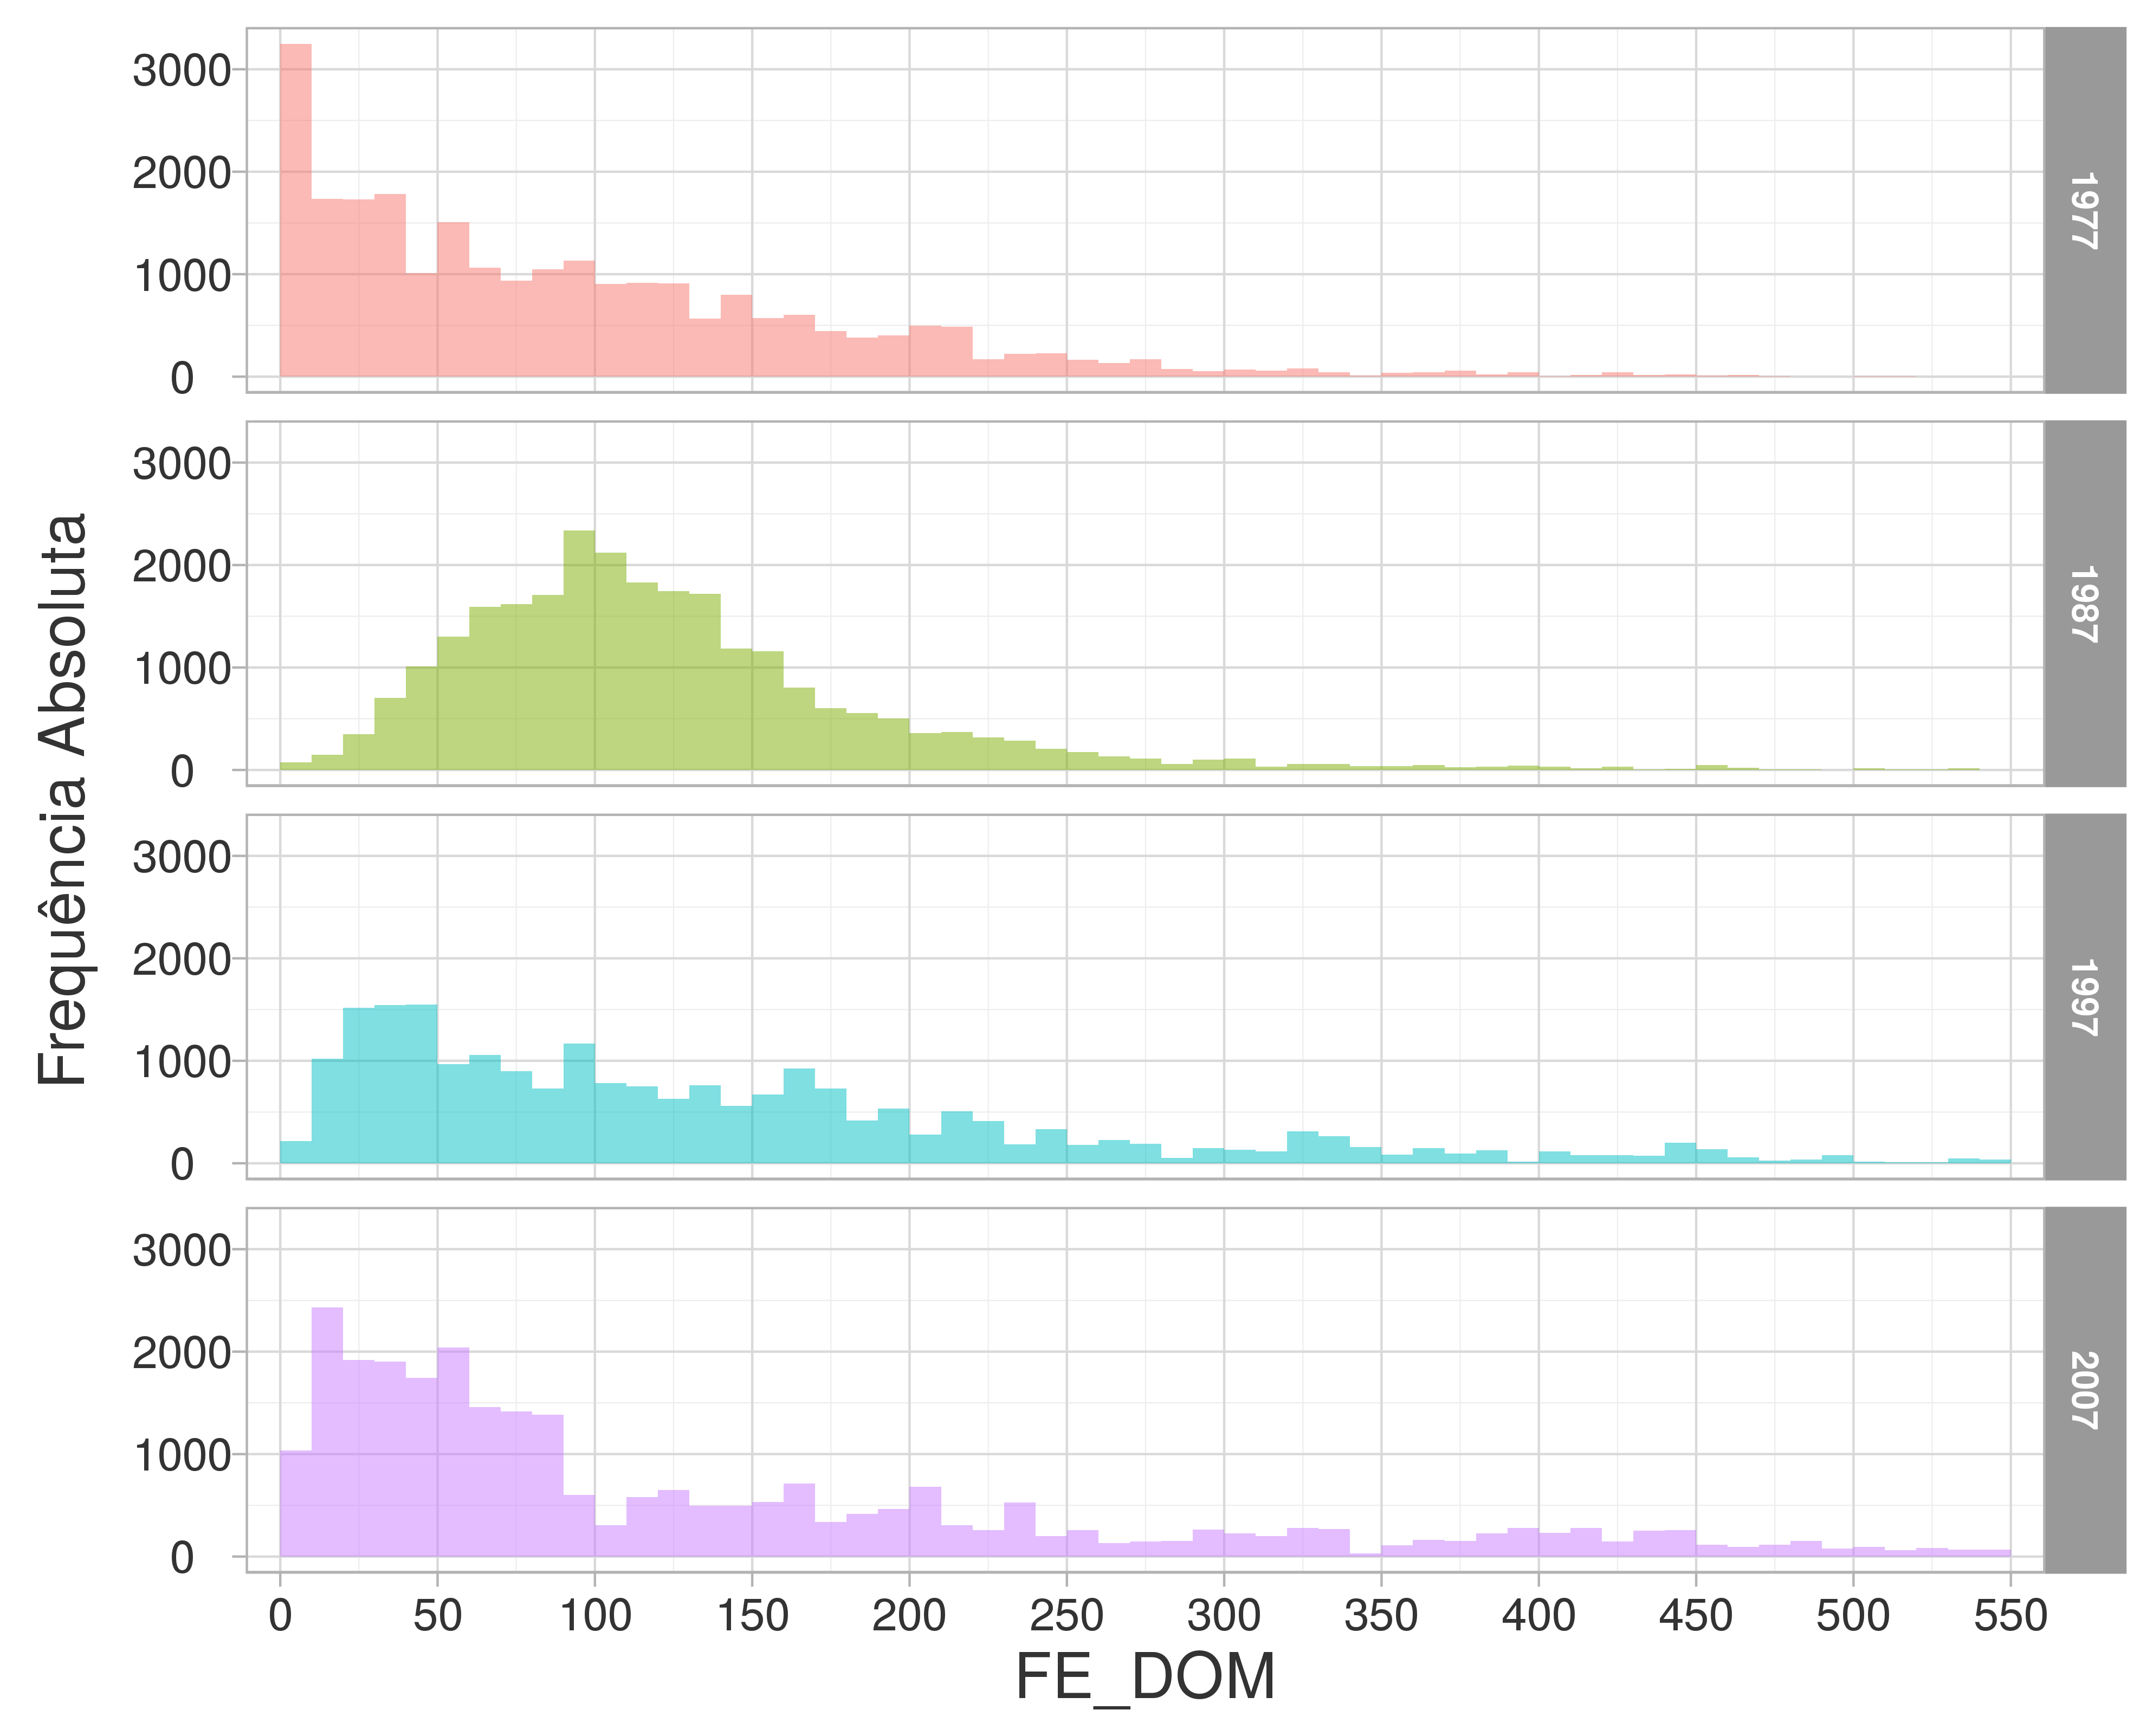
\includegraphics[width=1\textwidth]{./imagens/freq-abs-fe-dom.png}%
    \end{center}%
    %\fonte{Compilação própria}
\end{grafico}%


\clearpage

%\begin{table}[htb]
%\centering
%   \IBGEtab{%\renewcommand{\arraystretch}{1.5}%%\ABNTEXfontereduzida%
%        \renewcommand{\arraystretch}{1.5}
%        \caption{Estatísticas da variável ``FE_FAM''}
%        \label{tab:estat-fe-fam}
%    }{%
%
%    \begin{tabular}{cccccc}
%        \toprule
%        \textbf{ANO} & \textbf{Mínimo} & \textbf{1º Quartil} & \textbf{Mediana} & \textbf{3º Quartil} & \textbf{Máximo}  \\ \midrule \midrule
%        \textbf{1977}  & 0,50 & 24,77 &  68,49 & 137,90 & 1562,75 \\ \hline
%        \textbf{1987}  & 0,00 & 78,62 & 110,93 & 151,20 & 2210,00 \\ \hline
%        \textbf{1997}  & 1,00 & 49,26 & 109,54 & 200,05 & 2513,93 \\ \hline
%        \textbf{2007}  & 2,55 & 41,31 &  88,67 & 237,21 & 2256,41 \\ \hline
%        \textbf{Geral} & 0,00 & 48,00 &  99,37 & 172,85 & 2513,93 \\ \bottomrule
%        \textbf{ANO} & \textbf{Média} & \textbf{Desvio Padrão} & \textbf{Assimetria} & \textbf{Curtose} & \textbf{Nº de ``NA''}  \\ \midrule \midrule
%        \textbf{1977}  &  93,04 &  92,12 & 2,64 & 18,70 & 0 \\ \hline
%        \textbf{1987}  & 128,04 &  90,65 & 4,90 & 52,08 & 0 \\ \hline
%        \textbf{1997}  & 169,80 & 199,60 & 3,62 & 22,09 & 0 \\ \hline
%        \textbf{2007}  & 185,42 & 229,03 & 2,65 & 10,35 & 0 \\ \hline
%        \textbf{Geral} & 145,67 & 171,27 & 3,79 & 23,80 & 0 \\ \bottomrule
%        \end{tabular}
%    }
%
%\end{table}
%% Estatísticas para registros com F_FAM==1
%
%\begin{table}[htb]
%\centering
%   \IBGEtab{%\renewcommand{\arraystretch}{1.5}%%\ABNTEXfontereduzida%
%        \renewcommand{\arraystretch}{1.5}
%        \caption{Estatísticas da variável ``FE_PESS''}
%        \label{tab:estat-fe-pess}
%    }{%
%
%    \begin{tabular}{cccccc}
%        \toprule
%        \textbf{ANO} & \textbf{Mínimo} & \textbf{1º Quartil} & \textbf{Mediana} & \textbf{3º Quartil} & \textbf{Máximo}  \\ \midrule \midrule
%        \textbf{1977}  & 0,00 & 25,33 &  71,05 & 139,25 & 1562,75 \\ \hline
%        \textbf{1987}  & 0,00 & 79,46 & 111,78 & 151,24 & 2210,00 \\ \hline
%        \textbf{1997}  & 1,00 & 46,72 & 109,21 & 200,22 & 2516,28 \\ \hline
%        \textbf{2007}  & 2,92 & 48,25 & 111,45 & 296,24 & 2723,05 \\ \hline
%        \textbf{Geral} & 0,00 & 50,53 & 101,89 & 175,00 & 2723,05 \\ \bottomrule
%        \textbf{ANO} & \textbf{Média} & \textbf{Desvio Padrão} & \textbf{Assimetria} & \textbf{Curtose} & \textbf{Nº de ``NA''}  \\ \midrule \midrule
%        \textbf{1977}  &  95,10 &  94,15 & 2,76 & 20,84 & 0 \\ \hline
%        \textbf{1987}  & 128,58 &  90,56 & 4,78 & 49,15 & 0 \\ \hline
%        \textbf{1997}  & 170,00 & 203,37 & 3,69 & 23,14 & 0 \\ \hline
%        \textbf{2007}  & 213,72 & 260,38 & 2,81 & 12,60 & 0 \\ \hline
%        \textbf{Geral} & 148,76 & 177,83 & 4,14 & 29,04 & 0 \\ \bottomrule
%        \end{tabular}
%    }
%
%\end{table}
%% Estatísticas para registros com F_PESS==1

\clearpage
A variável \textbf{TIPO_DOM}, em 1977 e 1987, contava somente com as categorias ``particular'' e ``coletivo''; já em 1997 e 2007 passou a existir também a categoria favela, que foi agregada à categoria ``coletivo''. Foram adotadas as categorias coletivo e particular, de forma que funcionasse como uma \textbf{dummy} indicativa de domicílio particular (1) ou não (0). Quem não respondeu foi tratado como ``NA'', encerrando 4 domicílios (23 registros) em 1987, conforme pode ser observado na Tabela \ref{tab:estat-tipo-dom}. Nota-se que o percentual de moradias unifamiliares sempre permaneceu, em média, superior a 90\%.

\begin{table}[htb]
\centering
   \IBGEtab{%\renewcommand{\arraystretch}{1.5}%%\ABNTEXfontereduzida%
        \renewcommand{\arraystretch}{1.5}
        \caption{Estatísticas da variável ``TIPO_DOM''}
        \label{tab:estat-tipo-dom}
    }{%

    \begin{tabular}{cccccc}
        \toprule
        \textbf{ANO} & \textbf{1977} & \textbf{1987} & \textbf{1997} & \textbf{2007} & \textbf{Total}\\ \midrule \midrule
        \textbf{TIPO\_DOM=0}       &    148 &    207 &  2.054 &  1.195 &   3.604 \\ \hline
        \textbf{TIPO\_DOM=1}       & 24.465 & 25.859 & 21.787 & 28.762 & 100.873 \\ \hline
        \textbf{TIPO\_DOM=``NA''}  &      0 &      4 &      0 &      0 &       4 \\ \bottomrule
        \end{tabular}
    }

\end{table}
% Estatísticas para registros com F_DOM==1

A variável \textbf{TOT_FAM}, um dado de contagem, indica quantas famílias existem no domicílio e tem suas estatísticas descritivas apresentadas na Tabela \ref{tab:estat-tot-fam}. O valor médio indica haver pouco mais de uma família por domicílio, sendo a maior média de 1997 - dado coerente com a menor porcentagem de domicílios individuais (~91\%) indicada pela variável TIPO_DOM. A Figura \ref{fig:box-plot-tot-fam} mostra que a influência dos \textit{outliers} diminui com o tempo, o que também se reflete na queda dos desvios padrão, que indica menor dispersão dos dados.


\begin{figure}[htb]%
    \caption{\label{fig:box-plot-tot-fam}Box plot da variável ``TOT_FAM'', por ano}%
    \begin{center}%
        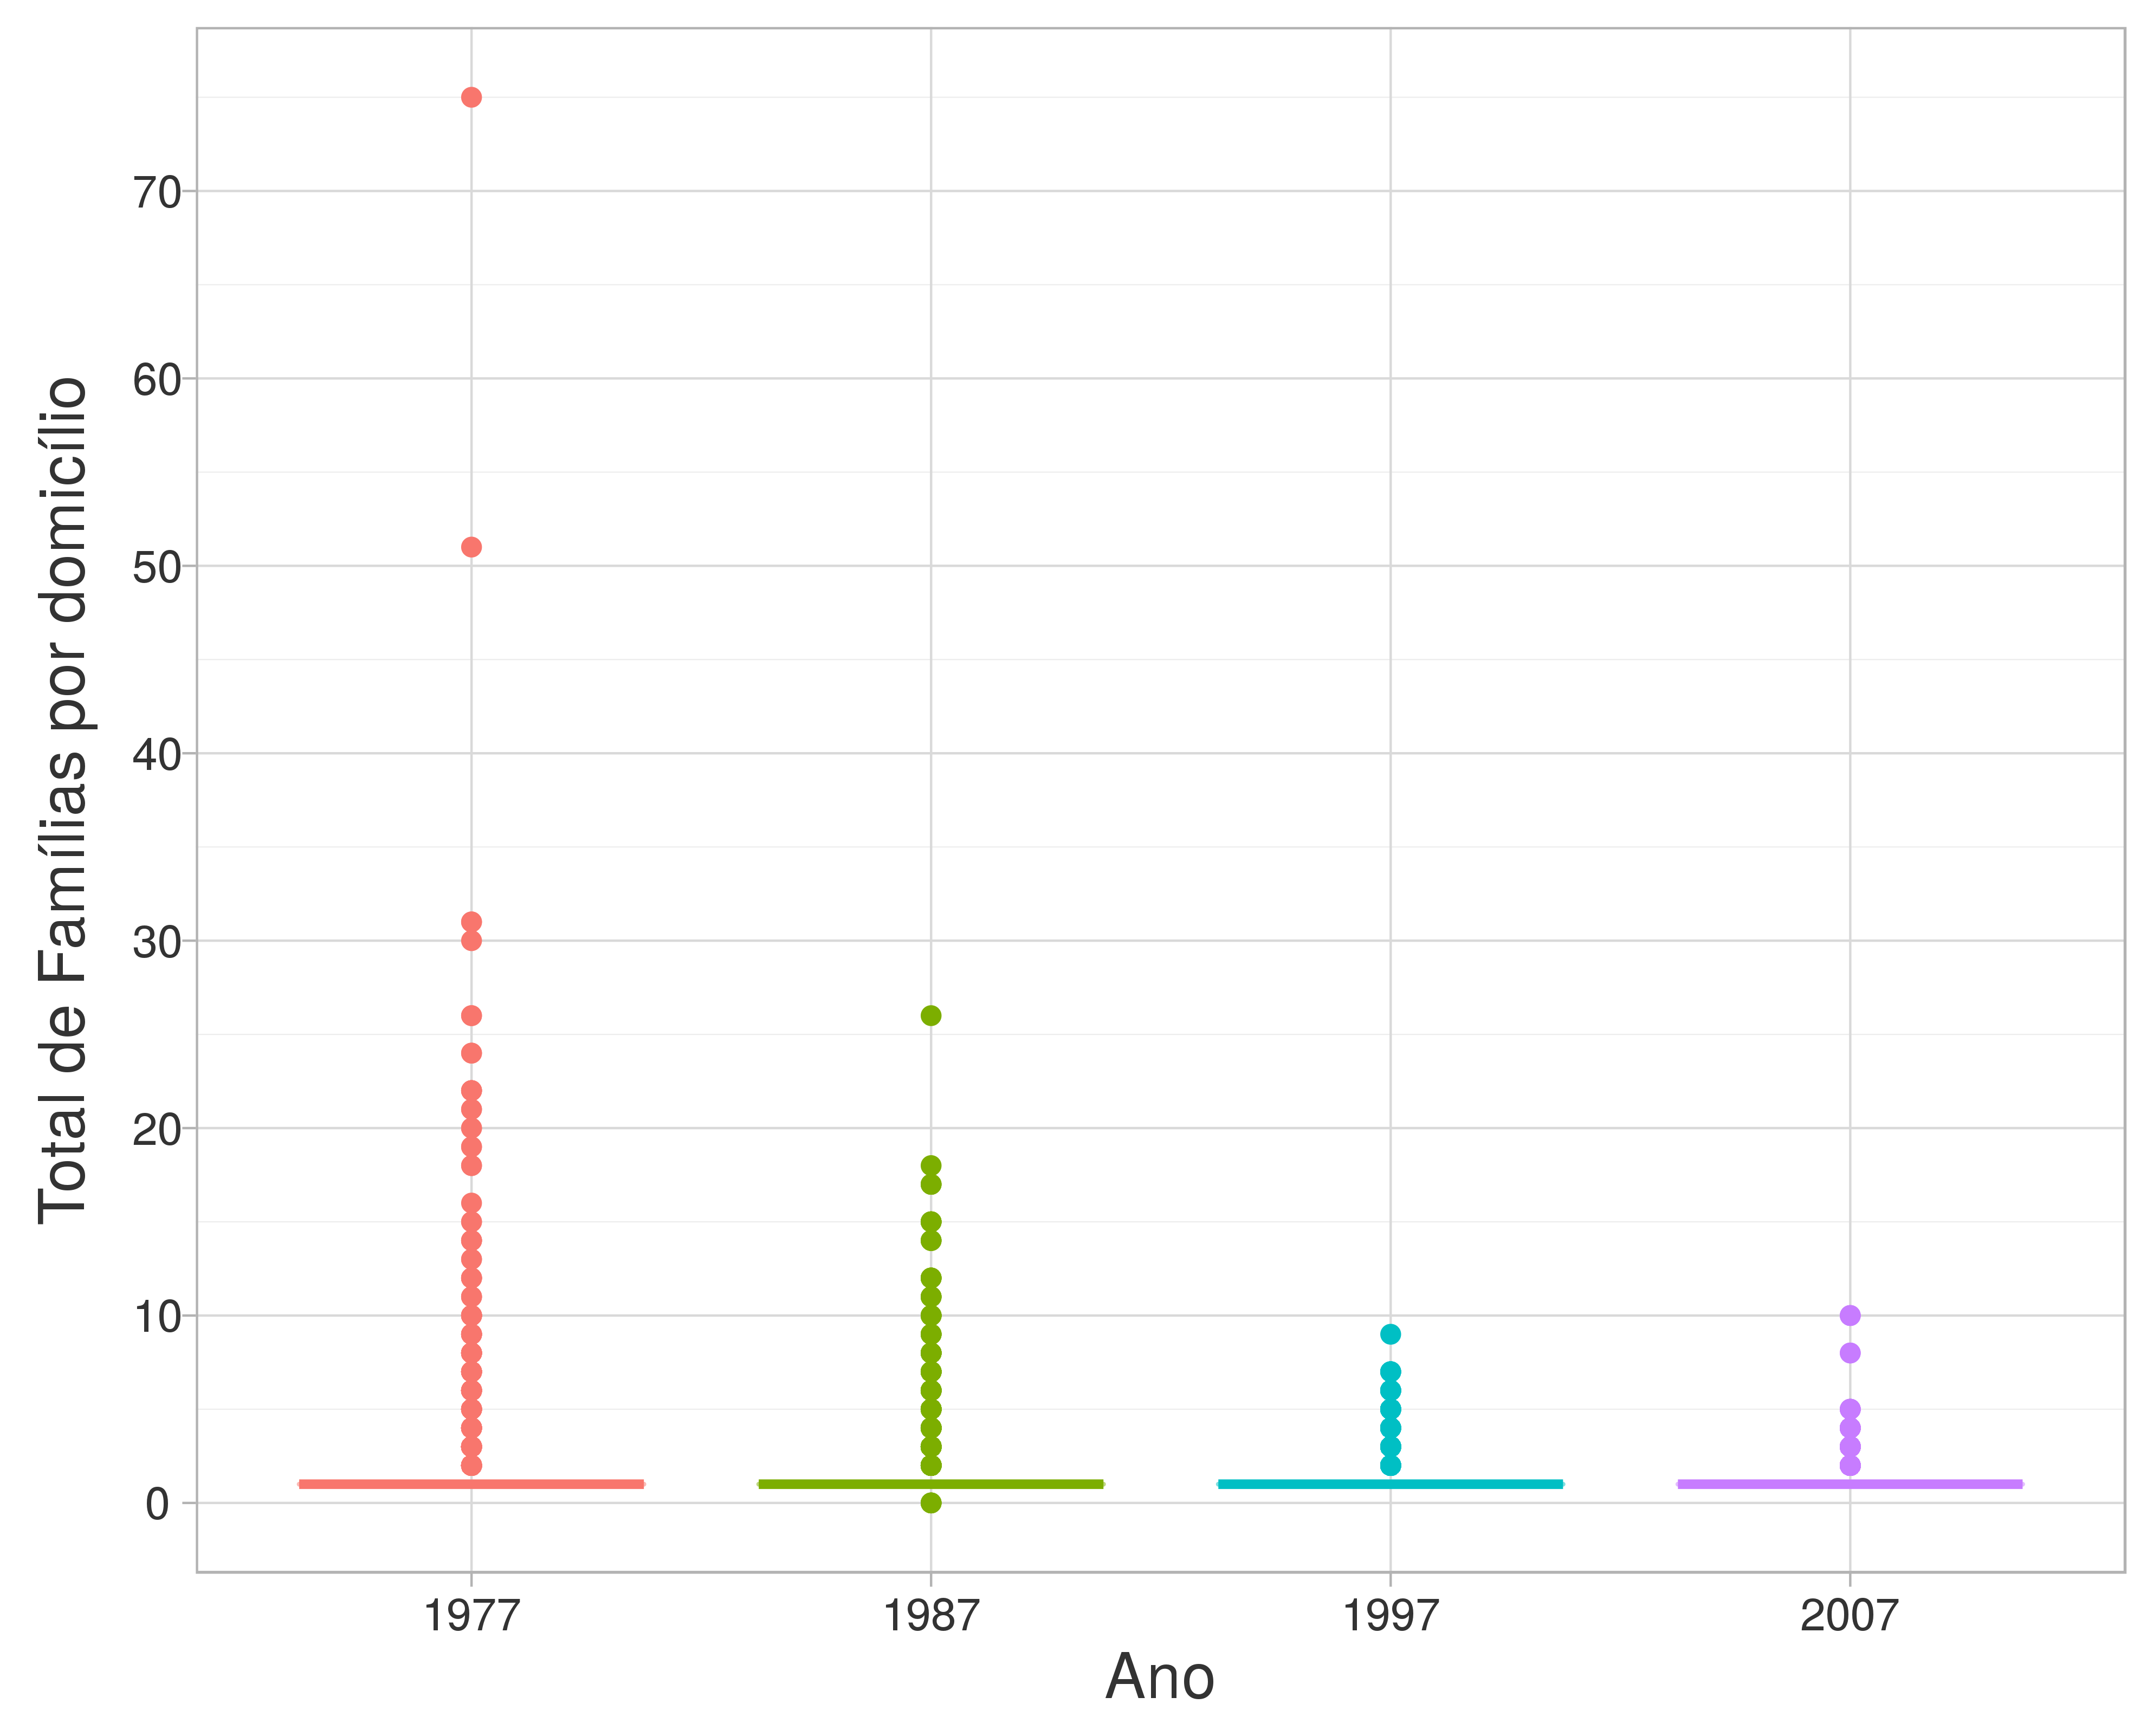
\includegraphics[width=1\textwidth]{./imagens/box-plot-tot-fam.png}%
    \end{center}%
    %\fonte{Compilação própria}
\end{figure}%

\begin{table}[htb]
\centering
   \IBGEtab{%\renewcommand{\arraystretch}{1.5}%%\ABNTEXfontereduzida%
        \renewcommand{\arraystretch}{1.5}
        \caption{Estatísticas da variável ``TOT_FAM''}
        \label{tab:estat-tot-fam}
    }{%

    \begin{tabular}{cccccc}
        \toprule
        \textbf{ANO} & \textbf{Média} & \textbf{Desvio Padrão} & \textbf{Assimetria} & \textbf{Curtose} & \textbf{Máximo}  \\ \midrule \midrule
        \textbf{1977}  & 1,08 & 0,99 & 33,70 & 1777,74 & 75 \\ \hline
        \textbf{1987}  & 1,12 & 0,61 & 13,72 & 306,37 & 26 \\ \hline
        \textbf{1997}  & 1,13 & 0,45 & 4,85 & 32,42 & 9 \\ \hline
        \textbf{2007}  & 1,03 & 0,23 & 14,00 & 346,13 & 10 \\ \hline
        \textbf{Geral} & 1,09 & 0,62 & 35,68 & 2734,92 & 75 \\ \bottomrule
        \end{tabular}
    }

\end{table}
% Estatísticas para registros com F_DOM==1


\newpage 

A variável \textbf{COND_MORA}, de natureza qualitativa, conta com três valores únicos, cujas frequências absolutas de registros de família são apresentada na Tabela \ref{tab:estat-cond-mora}. 
A categoria ``alugada'' (1) que em 1977 representava ~35\% da amostra, caiu para 23\% em 2007. A posse de residência (categoria ``própria'' - 2), subiu de 57\% para 68\% da amosta anual. A categoria ``outros'' (3), que abarca as categorias originais ``cedida'', ``outros'' e ``não se aplica'', oscila numa faixa próxima dos 10\%. Quem não respondeu foi tratado como ``NA'', encerrando 717 domicílios: 9 em 1977, 264 em 1987, 26 em 1997 e 460 em 2007.

\begin{table}[htb]
    \IBGEtab{%\renewcommand{\arraystretch}{1.5}%%\ABNTEXfontereduzida%
        \renewcommand{\arraystretch}{1.5}
        \caption{Estatísticas da variável ``COND_MORA''}
        \label{tab:estat-cond-mora}
    }{%

    \begin{tabular}{cccccc}
        \toprule
        \textbf{ANO} & \textbf{1977} & \textbf{1987} & \textbf{1997} & \textbf{2007} & \textbf{Total}\\ \midrule \midrule
        \textbf{COND_MORA=1}      &  9.174 &  7.967 &  5.168 &  7.268 & 29.577 \\ \hline
        \textbf{COND_MORA=2}      & 14.984 & 17.429 & 18.040 & 21.062 & 71.515 \\ \hline
        \textbf{COND_MORA=3}      &  1.990 &  2.557 &  3.611 &  2.065 & 10.223 \\ \hline
        \textbf{COND_MORA=``NA''} &      9 &    264 &     26 &    460 &    759 \\ \bottomrule
        \end{tabular}
    }

\end{table}
% Estatísticas para registros com F_FAM==1


Não foram mantidas no BDU as variáveis relativas aos bens de consumo, pois a função delas era servir de \emph{input} para determinar a renda atribuída (na ausência de declaração da renda), informação de que já se dispõe no banco de dados. Apenas os bens que são meios de transporte foram mantidos (automóveis, motocicletas e bicicletas) e serão explorados mais adiante.

Os valores monetários de renda familiar, renda individual e valor de estacionamento encontravam-se, em cada banco de dados, em um mês de referência diferente (segundo Quadro \ref{qua:atrib-renda}). Foram estudadas as possibilidades de correção pelos seguintes índices:

\begin{compactitem}
\item IPC-Brasil: índice de preços ao consumidor, que mede a variação de preços de um conjunto fixo de bens e serviços componentes de despesas habituais de famílias com nível de renda situado entre 1 e 33 salários mínimos mensais. Sua pesquisa de preços se desenvolve diariamente, cobrindo as sete principais capitais do país. Suas variações (DI, M e 10) referem-se ao período da coleta dos preços. A série histórica que se obteve de fontes oficiais (página da FGV e do Banco Central) não disponibilizava valores anteriores a 1989.

\item IGP: índice geral de preços, (a partir de 1950) é a média aritmética ponderada de três outros índices de preços (Índice de Preços ao Produtor Amplo (50\%), Índice de Preços ao Consumidor (30\%) e Índice Nacional de Custo da Construção (10\%). O IGP-M/FGV se refere ao período do dia vinte e um do mês anterior ao dia vinte do mês de referência e o IGP-DI/FGV se refere ao período do dia um ao dia trinta do mês em referência. A série histórica que se obteve de fontes oficiais (página da FGV e do Banco Central) não disponibilizava valores anteriores a 1989 para o IGP-M, ao passo que o IGP-DI
\footnote{Metodologia do IGP-DI disponível em: \url{http://portalibre.fgv.br/lumis/portal/file/fileDownload.jsp?fileId=8A7C82C54DB5CA9F014DD9322ADD306E} Acesso em 30 de agosto de 2015} dispunha de valores para correção desde a década de 1940.

\item IPCA: índice geral de preços ao consumidor amplo, que mede a variação de preços de um conjunto fixo de bens e serviços componentes de despesas habituais de famílias com nível de renda situado entre 1 e 40 salários mínimos mensais. Sua pesquisa de preços se desenvolve diariamente, cobrindo as dez principais capitais do país e Brasília. A série histórica que se obteve de fontes oficiais (página do IBGE e do Banco Central) divulga valores após dezembro de 1979. Sua variação IPCA-E é ainda mais recente (1991) e tem divulgação trimestral.

\item INPC: índice nacional de preços ao consumidor amplo, que mede a variação de preços de um conjunto fixo de bens e serviços componentes de despesas habituais de famílias com nível de renda situado entre 1 e 5 salários mínimos mensais. Sua pesquisa de preços se desenvolve continuamente, cobrindo as dez principais capitais do país e Brasília. A série histórica que se obteve de fontes oficiais (página do IBGE e do Banco Central) divulga valores após março de 1979.
\end{compactitem}

Assim, pela abrangência histórica foi utilizado o IPG-DI para levar os valores de setembro de 1977 para setembro de 1987. Estes valores, bem como os advindos da OD de 1987, foram levados a outubro de 2007 sofrendo correção do INPC. Este mesmo índice foi utilizado para levar os valores de outubro de 1997 a outubro de 2007. Escolheu-se o INPC, dentro os demais disponíveis, devido à faixa de abrangência da renda familiar utilizada em sua determinação. Não se quis priorizar índices cujas cestas tivessem um perfil de consumo alto, dado que as politicas de transporte público devem priorizar especialmente as menores faixas de renda. A composição final dos deflatores utilizados é apresentada na Tabela \ref{tab:deflatores}.

\begin{table}[htb]
    \IBGEtab{%\renewcommand{\arraystretch}{1.5}%%\ABNTEXfontereduzida%
        \renewcommand{\arraystretch}{1.5}
        \caption{Deflatores utilizados para correção dos valores monetários para outubro/2007}
        \label{tab:deflatores}
    }{%

    \begin{tabular}{ccccc}
        \toprule
        \textbf{ANO} & \textbf{1977} & \textbf{1987} & \textbf{1997} & \textbf{2007}\\ \midrule \midrule
        \textbf{Deflator} & 0,44234590 & 0,09664666 & 1,94136464 & 1  \\ \bottomrule
        \end{tabular}
    }

\end{table}


A renda familiar (variável \textbf{REN_FAM}) tem seus maiores valores de média e mediana em 1977, conforme Tabela \ref{tab:estat-ren-fam}, talvez por reflexo da época do ``milagre econômico brasileiro'', %TODO por referencia aqui 
comumente atribuído ao período do final dos anos 1960 até a metade dos anos 1970.
Após isso, 1987 apresenta a menor média e também queda da mediana; pode ser devido à recessão que marcou o Brasil nos anos 1980, quando se registraram baixo crescimento do PIB, %TODO por referencia aqui
alto nível de desemprego, %TODO por referencia aqui
perda do poder de compra da população, %TODO por referencia aqui 
e índices de inflação extremamente elevados. %TODO por referencia aqui
Em 1997, a média da renda familiar sobe, porém a mediana continua a cair, o que pode significar uma recuperação do aquecimento econômico, porém, sem frear o aprofundamento das desigualdades. %TODO por referencia aqui
Com o valor da média de 2007, parece realmente estar ocorrendo uma recuperação econômica (aumento da renda média familiar) e também uma redução das desigualdades (aumento da mediana da renda média familiar) - ver Gráfico \ref{graf:freq-rel-ren-fam}.


\begin{table}[htb]
\centering
   \IBGEtab{%\renewcommand{\arraystretch}{1.5}%%\ABNTEXfontereduzida%
        \renewcommand{\arraystretch}{1.5}
        \caption{Estatísticas da variável ``REN_FAM''}
        \label{tab:estat-ren-fam}
    }{%
    \begin{tabular}{cccccc}
        \toprule
        \textbf{ANO} & \textbf{Mínimo} & \textbf{1º Quartil} & \textbf{Mediana} & \textbf{3º Quartil} & \textbf{Máximo}  \\ \midrule \midrule
        \textbf{1977}  & 0 & 1.351,51 & 2.534,08 & 4.796,58 &  42.234,2 \\ \hline
        \textbf{1987}  & 0 &   875,62 & 1.523,44 & 2.801,21 &  61.830,1 \\ \hline
        \textbf{1997}  & 0 &   330,03 & 1.203,65 & 2.912,05 & 172.781,0 \\ \hline
        \textbf{2007}  & 0 & 1.144,82 & 2.080,00 & 4.000,00 &  46.000,0 \\ \hline
        \textbf{Geral} & 0 &   935,73 & 1.801,63 & 3.582,21 & 172.181,0 \\ \bottomrule
        \textbf{ANO} & \textbf{Média} & \textbf{Desvio Padrão} & \textbf{Assimetria} & \textbf{Curtose} & \textbf{Nº de ``NA''}  \\ \midrule \midrule
        \textbf{1977}  & 4.037,27 & 4.724,88 & 3,56 &  18,74 & 0 \\ \hline
        \textbf{1987}  & 2.393,58 & 2.826,96 & 4,06 &  29,85 & 0 \\ \hline
        \textbf{1997}  & 2.453,89 & 4.148,06 & 7,20 & 149,78 & 0 \\ \hline
        \textbf{2007}  & 3.186,19 & 3.312,25 & 2,85 &  13,73 & 0 \\ \hline
        \textbf{Geral} & 3.009,86 & 3.845,58 & 4,74 &  63,49 & 0 \\ \bottomrule
        \end{tabular}
    }

\end{table}
% Estatísticas para registros com F_FAM==1

\begin{grafico}[htb]%
    \caption{\label{graf:freq-rel-ren-fam}Distribuição da variável ``REN_FAM'', por ano}%
    \begin{center}%
        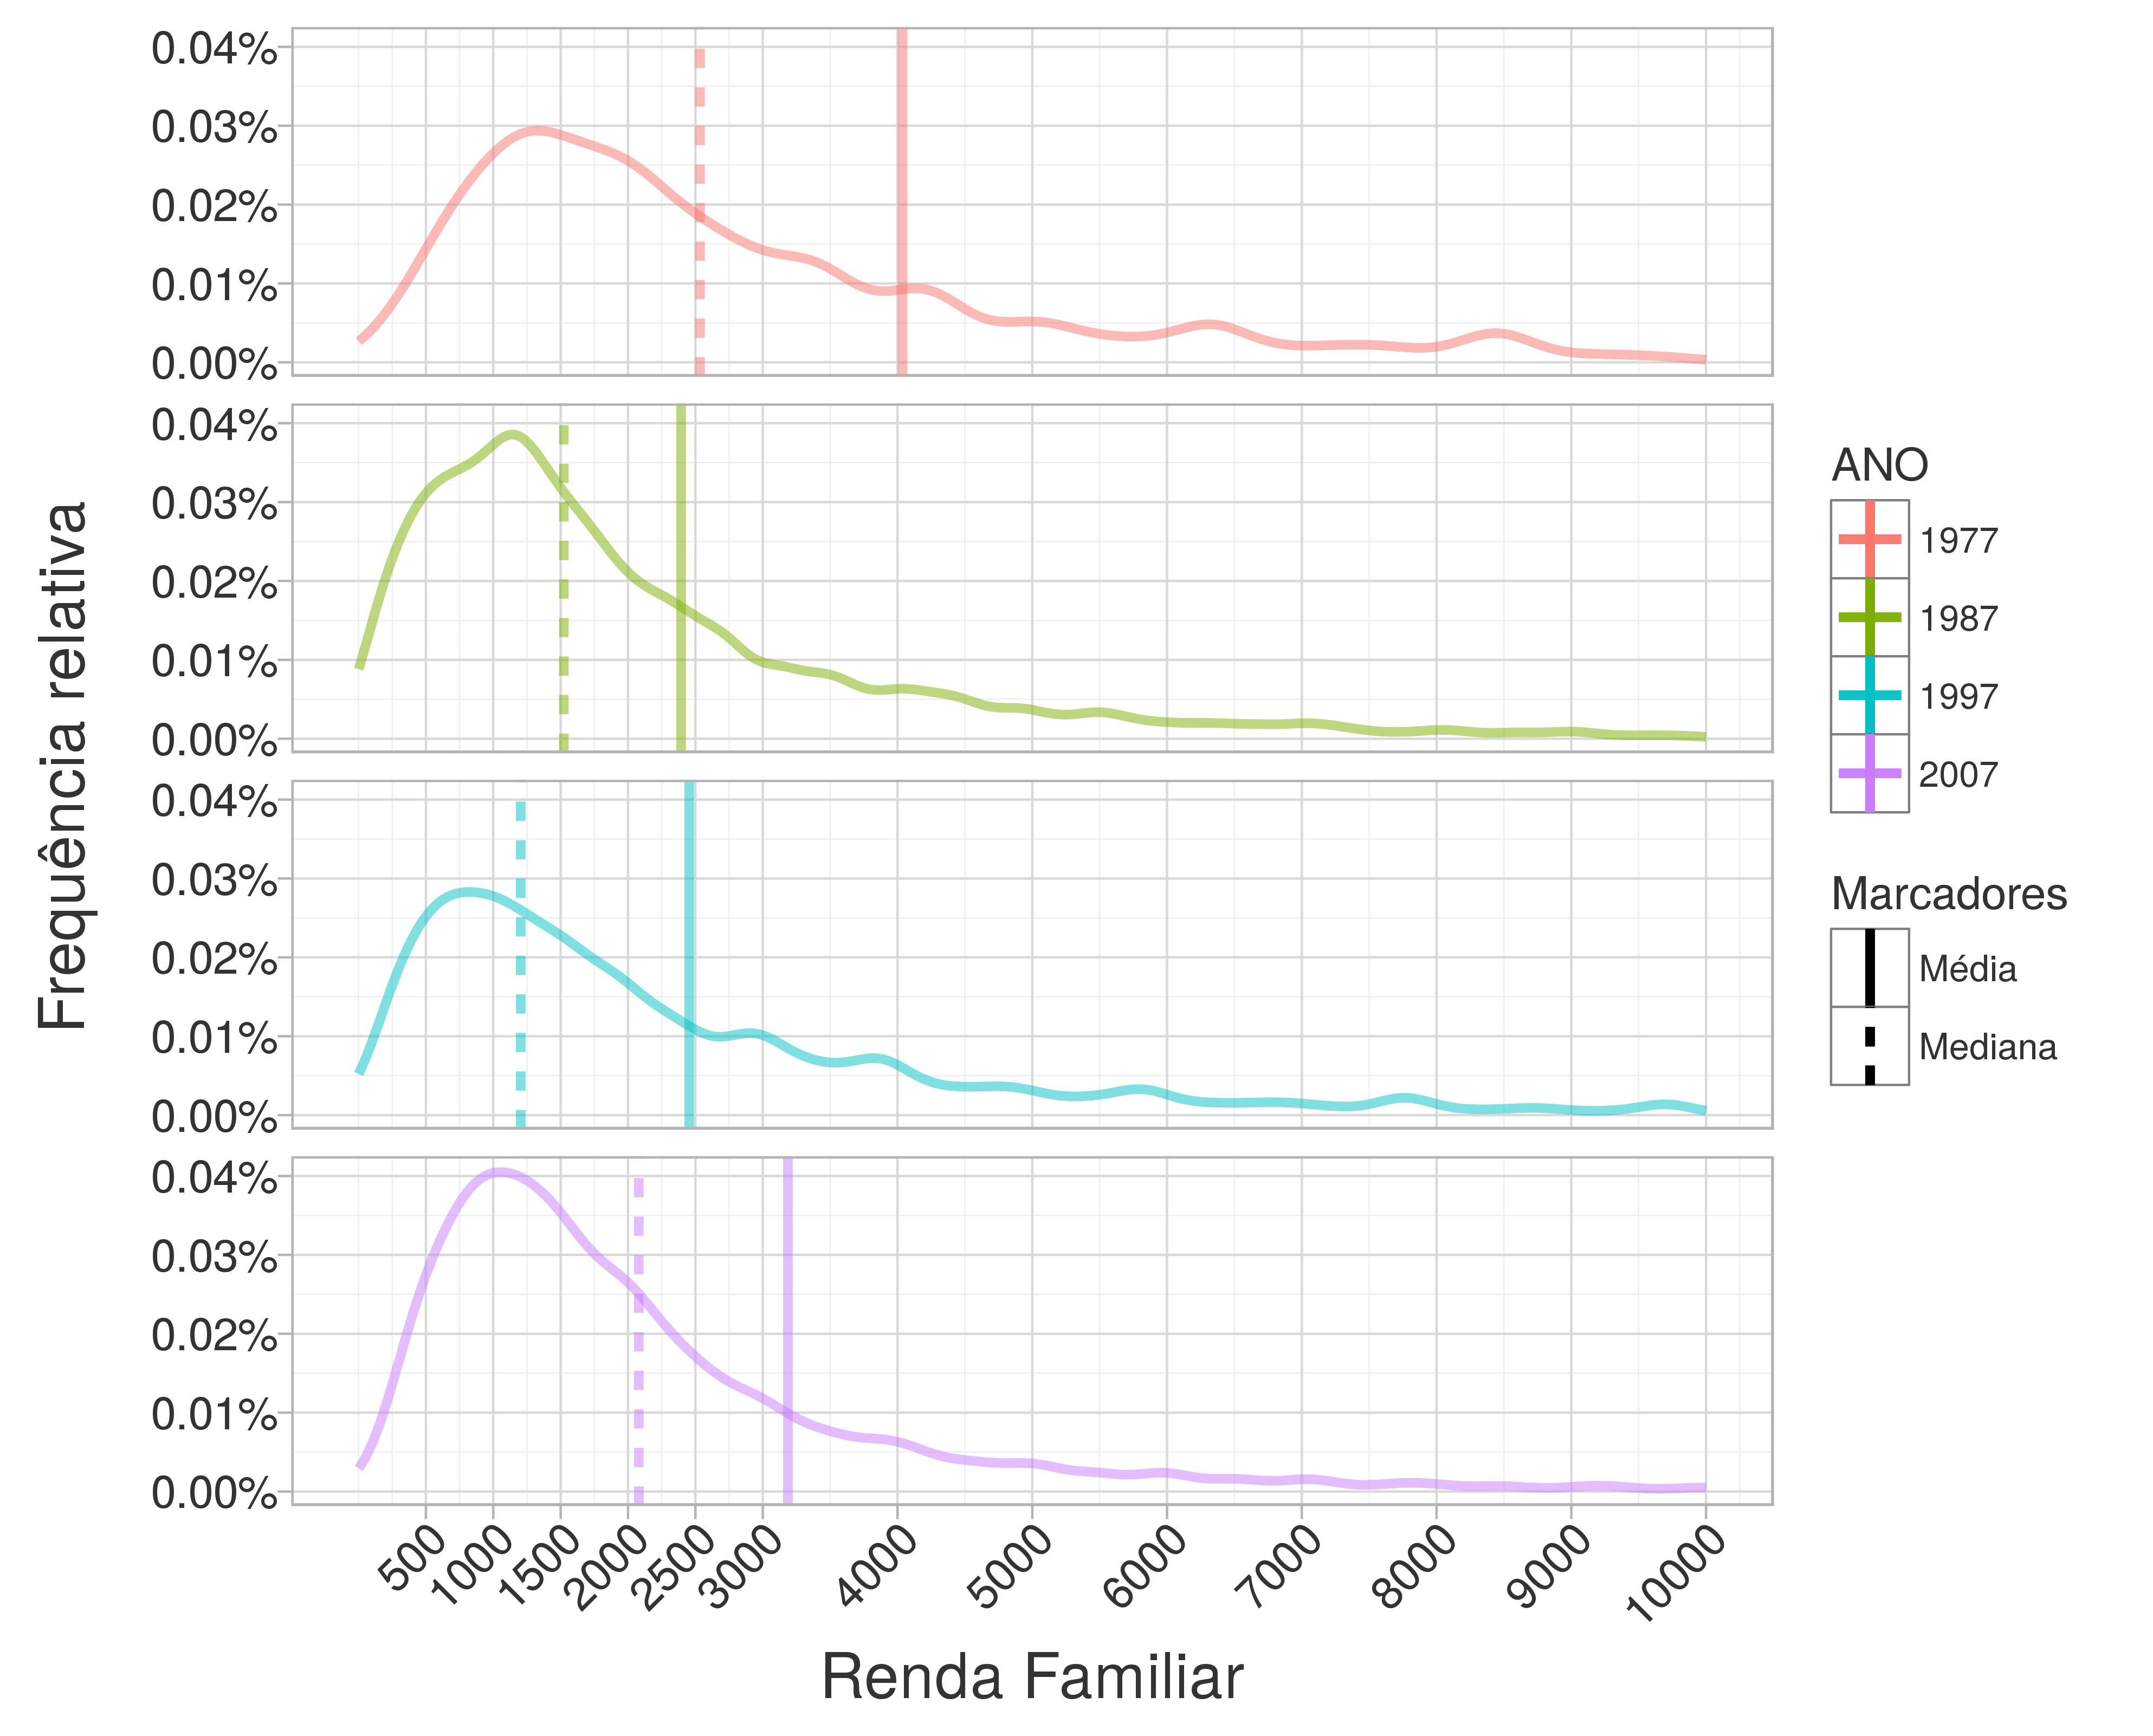
\includegraphics[width=1\textwidth]{./imagens/freq-rel-ren-fam.png}%
    \end{center}%
    %\fonte{Compilação própria}
\end{grafico}%

\clearpage
Para a construção do Gráfico \ref{graf:class-econ-ren-fam}, a partir da variável \textbf{FAIXA_REN_FAM}, foram retiradas as famílias que declararam renda nula. Posto isso, vê-se que as classes E e D, em 1977, correspondiam a 29\% da amostra. Em 1987 esse valor vai a 49\% e depois começa a decrescer para 45\% em 1997 e 37\% em 2007. A classe C (classe média) decresce de 1977 (~37\%) até 1997 (~33\%) e só aumenta novamente em 2007 (~36\%). Para estas classificações, foram utilizados sempre os valores em R\$ de outubro de 2007, bem como a classificação de classes econômicas vigente neste mesmo período.

\begin{grafico}[htb]%
    \caption{\label{graf:class-econ-ren-fam}Distribuição da variável ``FAIXA_REN_FAM'', por ano}%
    \begin{center}%
        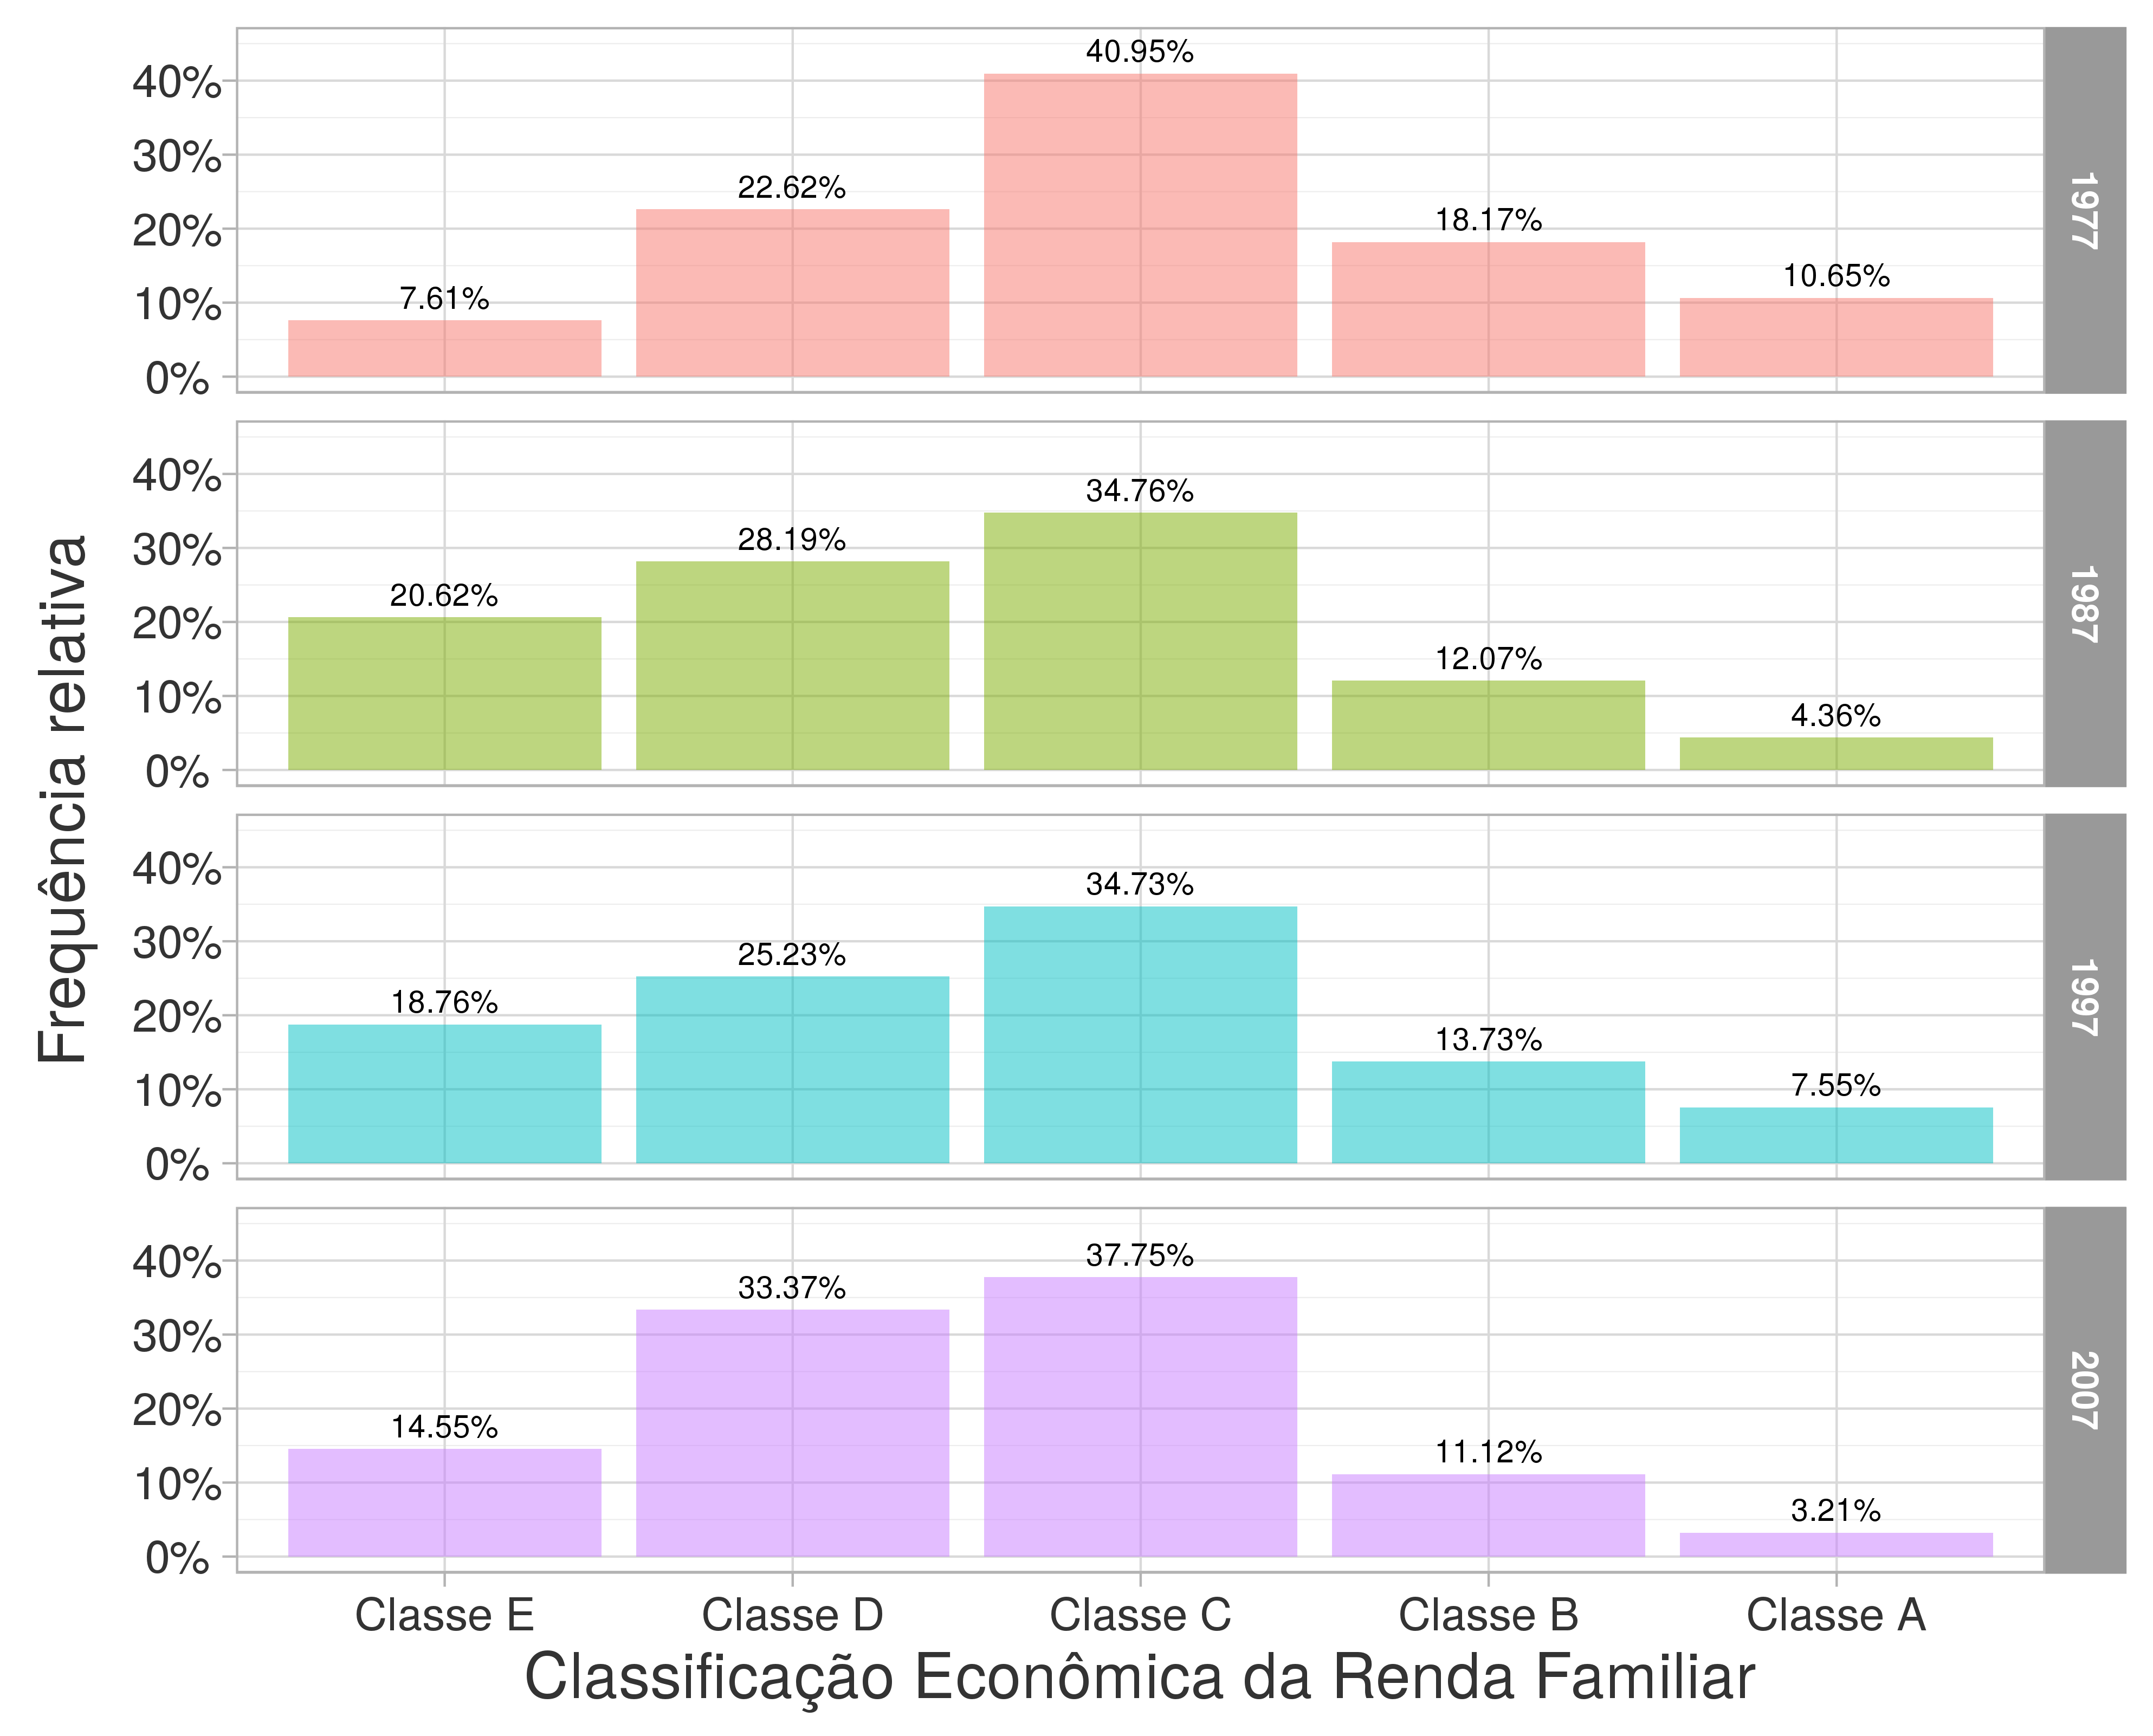
\includegraphics[width=1\textwidth]{./imagens/class-econ-ren-fam.png}%
    \end{center}%
    %\fonte{Compilação própria}
\end{grafico}%

Uma das variáveis que são \textit{proxy} da renda é a quantidade de automóveis na família (\textbf{QT_AUTO}).
As Tabelas \ref{tab:estat-frota} e \ref{tab:venda-veic-br} mostram que a frota de automóveis de uso familiar vem crescendo tanto no Brasil como na RMSP, assim como a motorização familiar (número de veículos por família) ao longo do tempo. Isto é, mesmo com o crescimento populacional do período, a aquisição de carros pelas famílias aumenta em taxa ainda maior.
A média de automóveis por família aumentou com o passar do tempo, conforme observa-se na coluna \textit{média} da Tabela \ref{tab:estat-qt-auto}.

\begin{table}[htb]
    \IBGEtab{%\renewcommand{\arraystretch}{1.5}%%\ABNTEXfontereduzida%
        \renewcommand{\arraystretch}{1.5}
        \caption{Evolução da frota de automóveis na RMSP segundo as Pesquisas OD}
        \label{tab:estat-frota}
    }{%

    \begin{tabular}{ccccc}
        \toprule
        \textbf{ANO} & \textbf{1977} & \textbf{1987} & \textbf{1997} & \textbf{2007}\\ \midrule \midrule
        \textbf{Frota} & 1.391.832 & 2.014.474 & 3.092.238 & 3.545.263  \\ \bottomrule
        \end{tabular}
    }

    \nota{Segundo o Departamento Estadual de Trânsito de São Paulo, em 2007 o município de São Paulo contava com cerca de 4,5 milhões de automóveis. Tal discrepância pode ocorrer porque os dados da CET levam em consideração, além dos veículos particulares, veículos de empresas, órgãos públicos, etc; e também por basear-se no cadastro do IPVA.}

\end{table}

\begin{table}[htb]
    \IBGEtab{%\renewcommand{\arraystretch}{1.5}%%\ABNTEXfontereduzida%
	    \renewcommand{\arraystretch}{1.5}
        \caption{Venda interna de veículos no Brasil entre 1960 e 2009}
		\label{tab:venda-veic-br}
    }{%
	    \begin{tabular}{c P{2.0cm} P{2.0cm} P{4.0cm}}
        \toprule
	           \headerCell{Ano} &
		       \headerCell{Autos} &
		       \headerCell{Total} &
		       \headerCell{Fator de crescimento (total)} \\
		    \midrule \midrule
		        1960&
		        40.980&
		        131.499&
		        1\\
		    \midrule
		        1970&
		        308.024&
		        416.704&
		        3,2\\
		    \midrule
		        1980&
		        739.028&
		        980.261&
		        7,5\\
		    \midrule
		        1990&
		        532.906&
		        712.741&
		        5,4\\
		    \midrule
		        2000&
		        1.176.774&
		        1.489.481&
		        11,3\\
		    \midrule
		        2009&
		        2.474.764&
		        3.141.240&
		        23,9\\
		    \bottomrule
		\end{tabular}
    }{%
		\fonte{Adaptado de \cite[p.29]{VASCONCELLOS2012}}
		}
\end{table}


\begin{table}[htb]
\centering
   \IBGEtab{%\renewcommand{\arraystretch}{1.5}%%\ABNTEXfontereduzida%
        \renewcommand{\arraystretch}{1.5}
        \caption{Estatísticas da variável ``QT_AUTO''}
        \label{tab:estat-qt-auto}
    }{%

    \begin{tabular}{cccccc}
        \toprule
        \textbf{ANO} & \textbf{Mínimo} & \textbf{1º Quartil} & \textbf{Mediana} & \textbf{3º Quartil} & \textbf{Máximo}  \\ \midrule \midrule
        \textbf{1977}  & 0 & 0 & 0 & 1 & 7 \\ \hline
        \textbf{1987}  & 0 & 0 & 0 & 1 & 9 \\ \hline
        \textbf{1997}  & 0 & 0 & 1 & 1 & 9 \\ \hline
        \textbf{2007}  & 0 & 0 & 1 & 1 & 8 \\ \hline
        \textbf{Geral} & 0 & 0 & 0 & 1 & 9 \\ \bottomrule
        \textbf{ANO} & \textbf{Média} & \textbf{Desvio Padrão} & \textbf{Assimetria} & \textbf{Curtose} & \textbf{Nº de ``NA''}  \\ \midrule \midrule
        \textbf{1977}  & 0,65 & 0,81 & 1,36 & 2,28 & 0 \\ \hline
        \textbf{1987}  & 0,57 & 0,77 & 1,59 & 4,09 & 0 \\ \hline
        \textbf{1997}  & 0,72 & 0,89 & 1,57 & 3,78 & 0 \\ \hline
        \textbf{2007}  & 0,78 & 0,86 & 1,19 & 1,99 & 0 \\ \hline
        \textbf{Geral} & 0,68 & 0,84 & 1,43 & 3,03 & 0 \\ \bottomrule
        \end{tabular}
    }

\end{table}
% Estatísticas para registros com F_FAM==1

\clearpage
Diversos estudos foram realizados para a construção de modelos desagregados que explicassem a posse de autos
\cite{RYAN1999, DARGAY1999, DARGAY2001, CHU2002, KARLAFTIS2002, PFEIFFER2005}.
É comum a utilização de variáveis como renda, número de trabalhadores, tamanho da família, número de estudantes, presença ou não de crianças na família, sexo e idade da pessoa responsável pela família. Embora não seja o foco deste estudo modelar a posse de autos pelas famílias, compreender o que influencia a motorização é importante porque a motorização influencia diretamente a mobilidade dos indivíduos.
\citeauthoronline{PFEIFFER2005} (\citeyear{PFEIFFER2005}), que analisam a evolução da motorização da RMSP entre 1987 e 1997, concluem que, para explicar a posse de autos ``\textit{as variáveis de estrutura familiar utilizadas na análise e modelagem da posse de autos perderam importância ao longo do tempo, assim como a própria renda familiar}''. Eles sugerem que isso pode ter se dado pela maior facilidade de financiamentos para aquisição de automóveis por uma família, ou ainda pela evolução das condições do transporte público, assim como da organização espacial da região metropolitana.

Segundo a Tabela \ref{tab:distr-autos-fam}, percebe-se que a proporção de famílias sem automóvel particular oscilou entre os anos, mantendo ainda assim uma tendência de queda entre 1977 e 2007. Oscilação entre os anos também ocorreu na proporção das famílias com dois ou mais automóveis, com tendência de crescimento entre 1977 e 2007. O comportamento mais consistente com os cenários macro econômicos brasileiros foi o das famílias com um automóvel: tiveram leve queda na posse de um automóvel em 1987 (década de crise econômica), aumento de pouco mais de 10\% em 1997 (após a estabilização da moeda em 1994), e aumento tímido (0,3\%) em 2007.

Foram criadas duas \textit{dummies} relativas à presença de automóveis na famílias: (i) presença de 1 automóvel e (ii) presença de 2 ou mais automóveis.
Segmentando as famílias segundo o sexo da pessoa responsável e analisando as frequências relativas da posse de autos através dessas \textit{dummies}, obtém-se o Gráfico \ref{graf:autos-sit-fam-sexo}. Nele observa-se que as variações da posse de autos das famílias cujos responsáveis são homens são semelhantes às daquelas cujas responsáveis são mulheres. Porém, as famílias que possuem 2 ou mais automóveis e cujos responsáveis são homens, tiveram uma leve queda de 2 pontos percentuais, enquanto as com dois ou mais automóveis chefiadas por mulheres apresentaram um aumento de 4 pontos percentuais.

Mas o grande destaque no que se refere à posse de automóvel das famílias pode ser dado ao par formado pela queda de 12 pontos percentuais para famílias sem automóvel e pelo aumento de 8 pontos percentuais para famílias com posse de um automóvel, ambos casos são de famílias chefiadas por mulheres e com tendência a continuar seus movimentos de queda e crescimento, respectivamente.

\begin{table}[htb]
\centering
   \IBGEtab{%\renewcommand{\arraystretch}{1.5}%%\ABNTEXfontereduzida%
        \renewcommand{\arraystretch}{1.5}
        \caption{Proporção das famílias segundo posse de automóveis e de acordo com sexo da pessoa responsável}
        \label{tab:distr-autos-fam}
    }{%

    \begin{tabular}{ccccccc}
        \toprule
	        \multirow{2}{*}{\quebraLinhaCel{\textbf{Sexo da Pessoa}\\ \textbf{Responsável}}} &
	        \multirow{2}{*}{\textbf{Posse de auto}} & \multicolumn{4}{c}{\textbf{ANO}} &
	        \multirow{2}{*}{\textbf{Geral (\%)}} \\
        \cline{3-6}
	        & & \textbf{1977 (\%)} & \textbf{1987 (\%)} & \textbf{1997 (\%)} & \textbf{2007 (\%)} &
	        \\
	      \midrule \midrule
  	      \multirow{3}{*}{\textbf{Feminino}} &
  	      \textbf{0 autos} &
  	      77,36 & 75,83 & 70,21 & 65,23 & 69,21 \\
  	    \cline{3-7}
  	       & \textbf{1 auto} &
  	      19,35 & 19,92 & 24,31 & 27,72 & 24,90 \\
  	    \cline{3-7}
  	       & \textbf{2 ou + autos} &
  	      3,29 & 4,25 & 5,48 & 7,05 & 5,89 \\
  	    \hline
  	      \multirow{3}{*}{\textbf{Masculino}} &
  	      \textbf{0 autos} &
  	      52,33 & 53,15 & 43,90 & 44,27 & 47,64 \\
  	    \cline{3-7}
  	       & \textbf{1 auto} &
  	      36,36 & 35,59 & 40,70 & 42,57 & 39,32 \\
  	    \cline{3-7}
  	       & \textbf{2 ou + autos} &
  	      11,31 & 11,26 & 15,39 & 13,16 & 13,04 \\
  	    \hline
  	      \multirow{3}{*}{\textbf{Geral}} &
  	      \textbf{0 autos} &
  	      55,70 & 56,92 & 49,37 & 51,25 & 52,65 \\
  	    \cline{3-7}
  	       & \textbf{1 auto} &
  	      34,07 & 33,00 & 37,30 & 37,62 & 35,98 \\
  	    \cline{3-7}
  	       & \textbf{2 ou + autos} &
  	      10,23 & 10,08 & 13,33 & 11,12 & 11,38 \\
        \bottomrule
        \end{tabular}
    }

\end{table}
% Estatísticas para registros com F_FAM==1

\begin{grafico}[htb]%
    \caption{\label{graf:autos-sit-fam-sexo} Proporção de famílias com pessoa responsável do sexo feminino e do sexo masculino, segundo posse de automóveis, por ano}%
    \begin{center}%
        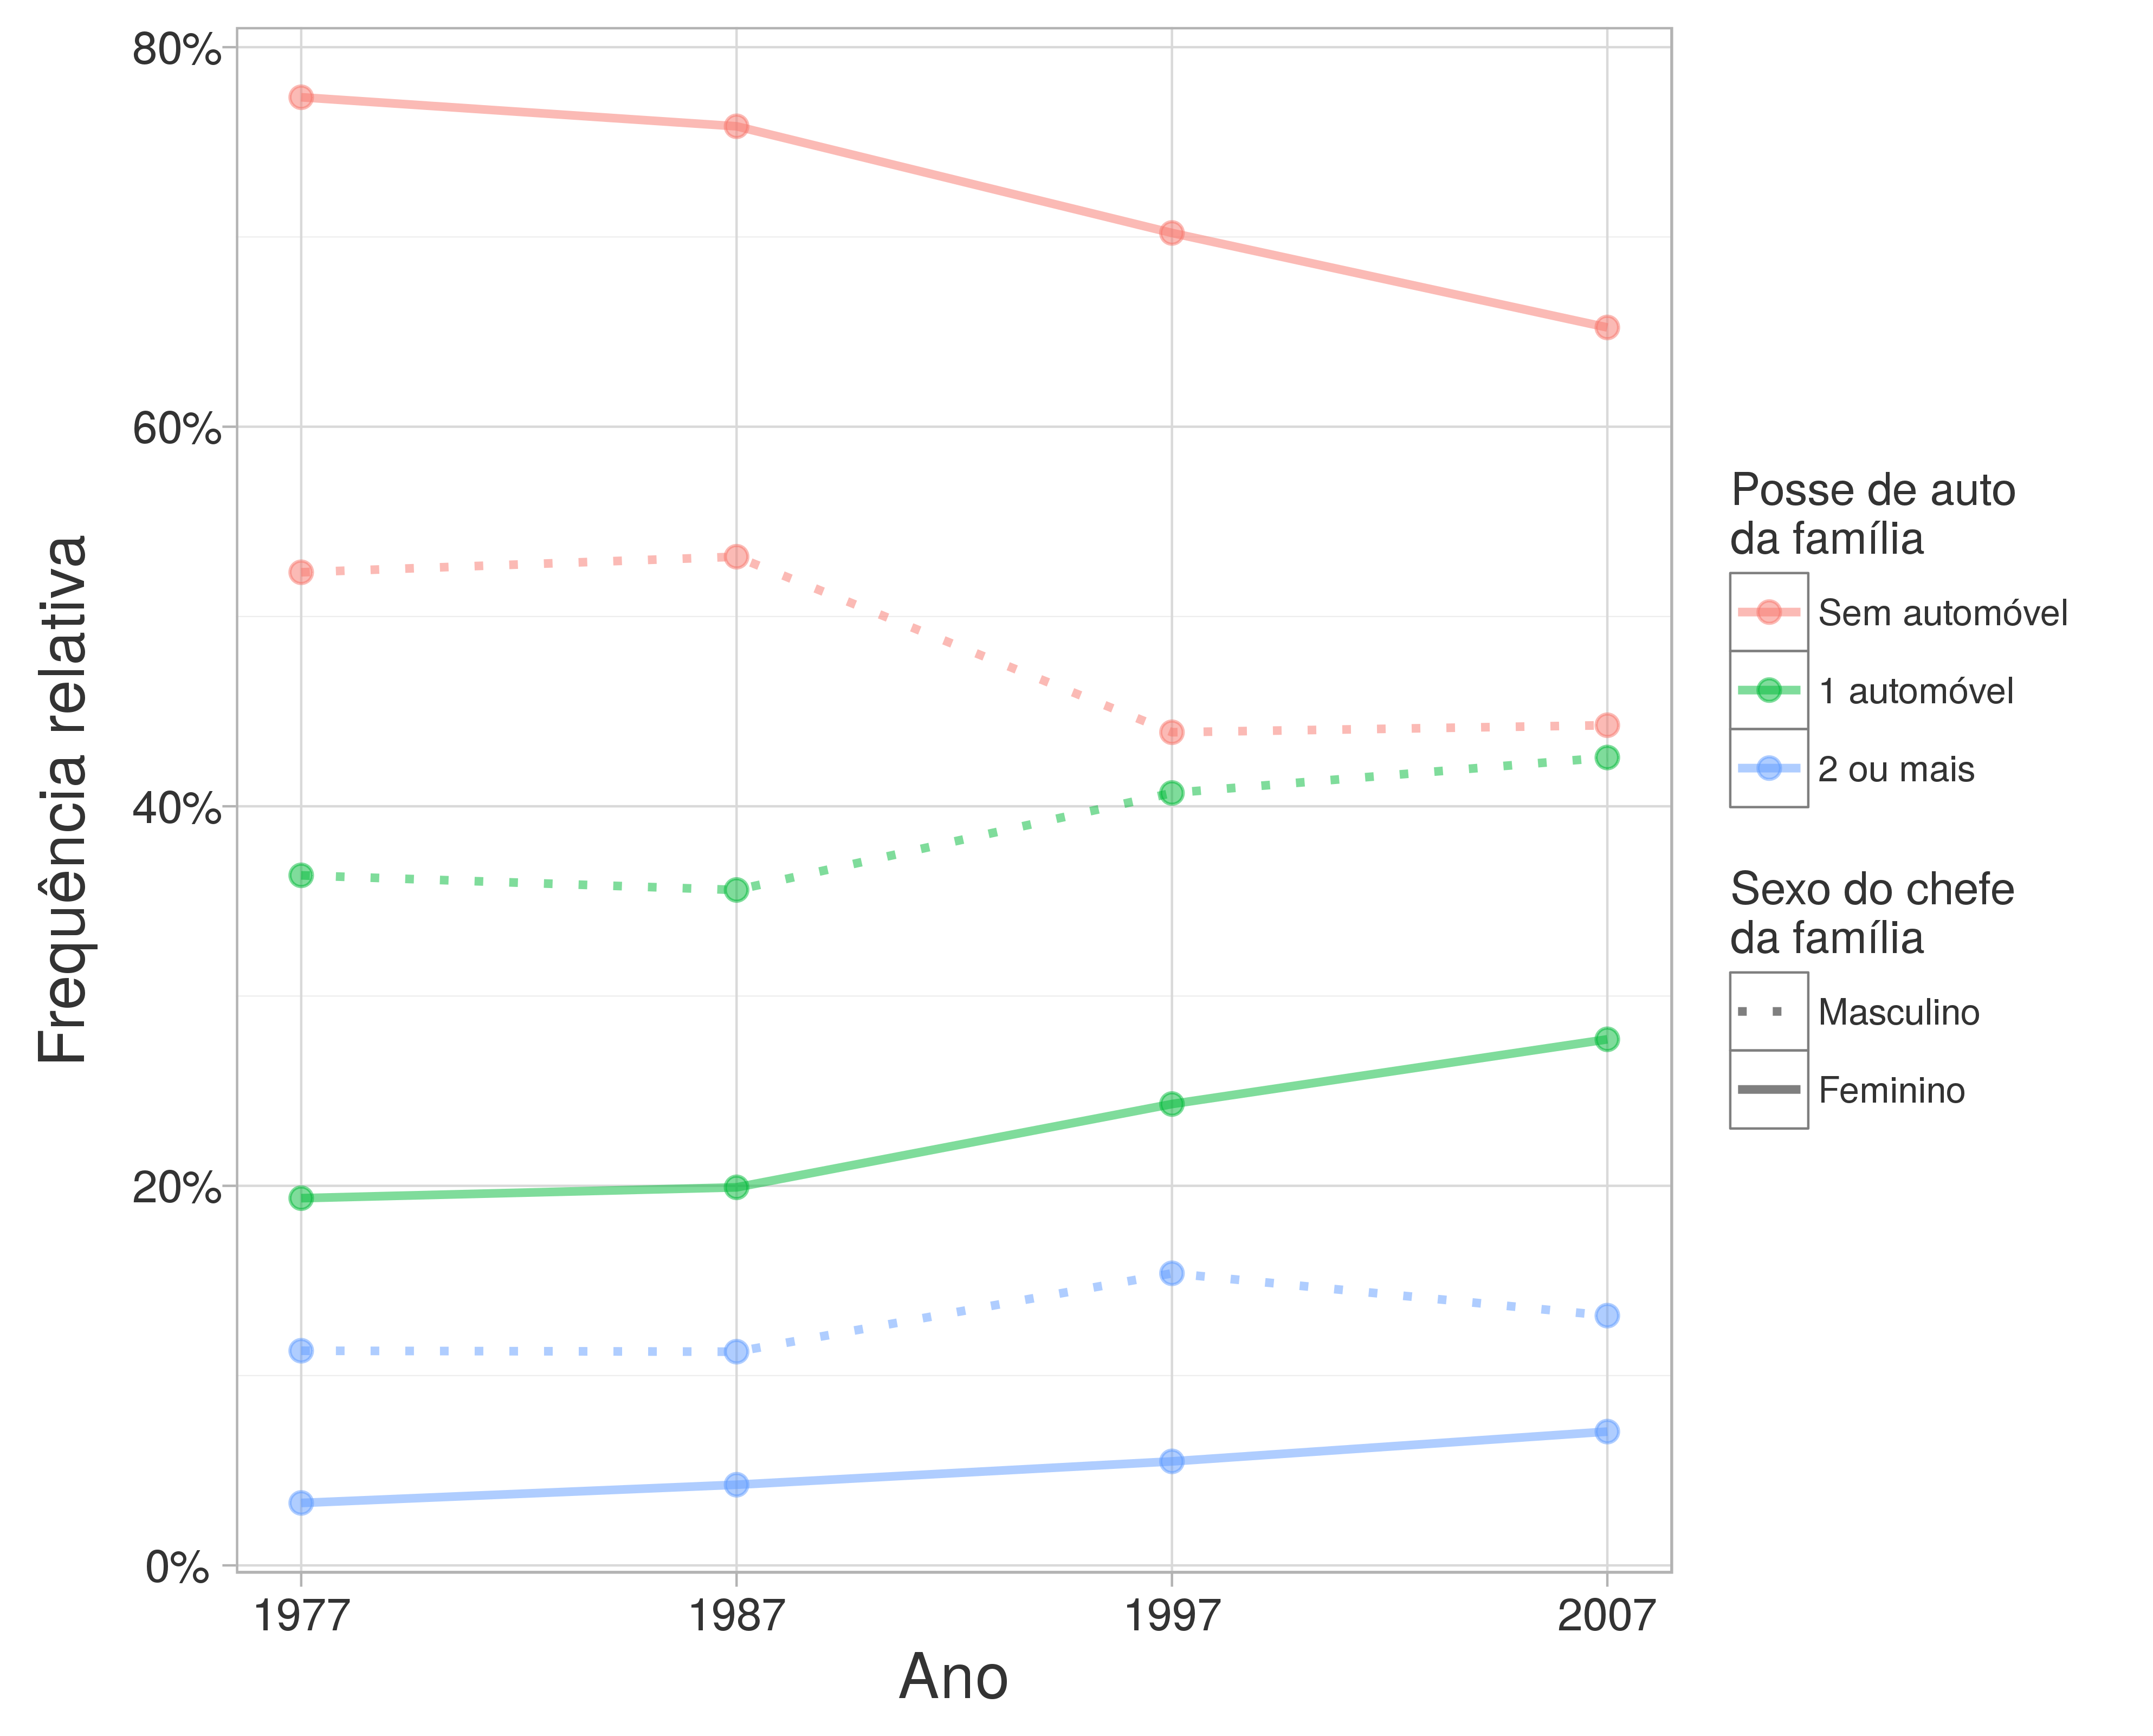
\includegraphics[width=1\textwidth]{./imagens/autos-sit-fam-sexo.png}%
    \end{center}%
    %\fonte{Compilação própria}
\end{grafico}%

\clearpage
A quantidade de motocicletas (\textbf{QT_MOTO}) e bicicletas (\textbf{QT_BICI}) foram levantadas apenas na Pesquisa OD de 2007, e têm suas estatísticas descritivas são apresentadas na Tabela \ref{tab:estat-qt-moto-bici}.
Percebe-se que, embora um meio de transporte individual motorizado mais barato, a incidência da posse de motocicletas é uma fenômeno mais raro, provavelmente devido ao risco associado a esse meio de transporte.

Essa falta de segurança na condução do meio de transporte também ocorre com a bicicleta, porém, além de ser ainda mais barata que a motocicleta, ela não é motorizada e, por isso, comumente trafega nos passeios públicos e calçadas, onde o(a) condutor(a) sofre menor risco de colisão com meios motorizados de transporte (motocicletas, carros, ônibus e caminhões). Com a recente política municipal de incentivo à bicicleta como meio de transporte, por meio de investimentos em infraestrutura cicloviária, é possível que na Pesquisa OD de 2017 haja evoluções destes dados que mereçam investigação.
Vale lembrar que existe também a questão do status associado muito mais fortemente à posse do automóvel do que da motocicleta; e no caso das bicicletas, seu uso é associado à ideia de pobreza e falta de recursos suficientes para comprar um carro.
%TODO por referências aqui

\begin{table}[htb]
\centering
   \IBGEtab{%\renewcommand{\arraystretch}{1.5}%%\ABNTEXfontereduzida%
        \renewcommand{\arraystretch}{1.5}
        \caption{Estatísticas das variáveis ``QT_MOTO'' e ``QT_BICI''}
        \label{tab:estat-qt-moto-bici}
    }{%

    \begin{tabular}{cccccc}
        \toprule
        \textbf{2007} & \textbf{Mínimo} & \textbf{1º Quartil} & \textbf{Mediana} & \textbf{3º Quartil} & \textbf{Máximo}  \\ \midrule \midrule
        \textbf{motocicleta}  &  0 &  0 &  0 &  0 &  9 \\ \hline
        \textbf{bicicleta} &  0 &  0 &  0 &  1 &  9 \\ \bottomrule
        \textbf{2007} & \textbf{Média} & \textbf{Desvio Padrão} & \textbf{Assimetria} & \textbf{Curtose} & \textbf{Nº de ``NA''}  \\ \midrule \midrule
        \textbf{motocicleta}  & 0,07 & 0,29 & 5,86 & 74,31 & 0 \\ \hline
        \textbf{bicicleta} & 0,46 & 0,8 & 2,27 & 7,5 & 0 \\ \bottomrule
        \end{tabular}
    }

\end{table}
% Estatísticas para registros com F_FAM==1

A variável \textbf{TOT_PESS}, um dado de contagem, indica quantas pessoas existem na família e tem suas estatísticas descritivas apresentadas na Tabela \ref{tab:estat-tot-pess}. Não havia \textit{missing values} e o valor médio indica que o tamanho da família diminuiu, passando de pouco mais de 4 pessoas em 1977 para pouco menos de 3 pessoas por família em 2007.
Em comportamento análogo a TOT_FAM, a Figura \ref{fig:box-plot-tot-pess} indica que a influência dos \textit{outliers} de TOT_PESS diminui com o tempo, o que também se reflete na queda dos desvios padrão, que indica menor dispersão dos dados.

\begin{table}[htb]
\centering
   \IBGEtab{%\renewcommand{\arraystretch}{1.5}%%\ABNTEXfontereduzida%
        \renewcommand{\arraystretch}{1.5}
        \caption{Estatísticas da variável ``TOT_PESS''}
        \label{tab:estat-tot-pess}
    }{%

    \begin{tabular}{cccccc}
        \toprule
        \textbf{ANO} & \textbf{Média} & \textbf{Desvio Padrão} & \textbf{Assimetria} & \textbf{Curtose} & \textbf{Máximo}  \\ \midrule \midrule
        \textbf{1977}  & 4,13 & 2,09 & 0,99 & 1,78 & 18 \\ \hline
        \textbf{1987}  & 3,93 & 1,80 & 0,92 & 2,03 & 22 \\ \hline
        \textbf{1997}  & 3,68 & 1,73 & 0,82 & 1,68 & 17 \\ \hline
        \textbf{2007}  & 2,96 & 1,46 & 0,78 & 1,00 & 14 \\ \hline
        \textbf{Geral} & 3,65 & 1,83 & 1,00 & 2,10 & 22 \\ \bottomrule
        \end{tabular}
    }

\end{table}
% Estatísticas para registros com F_FAM==1


\begin{figure}[htb]%
    \caption{\label{fig:box-plot-tot-pess}Box plot da variável ``TOT_PESS'', por ano}%
    \begin{center}%
        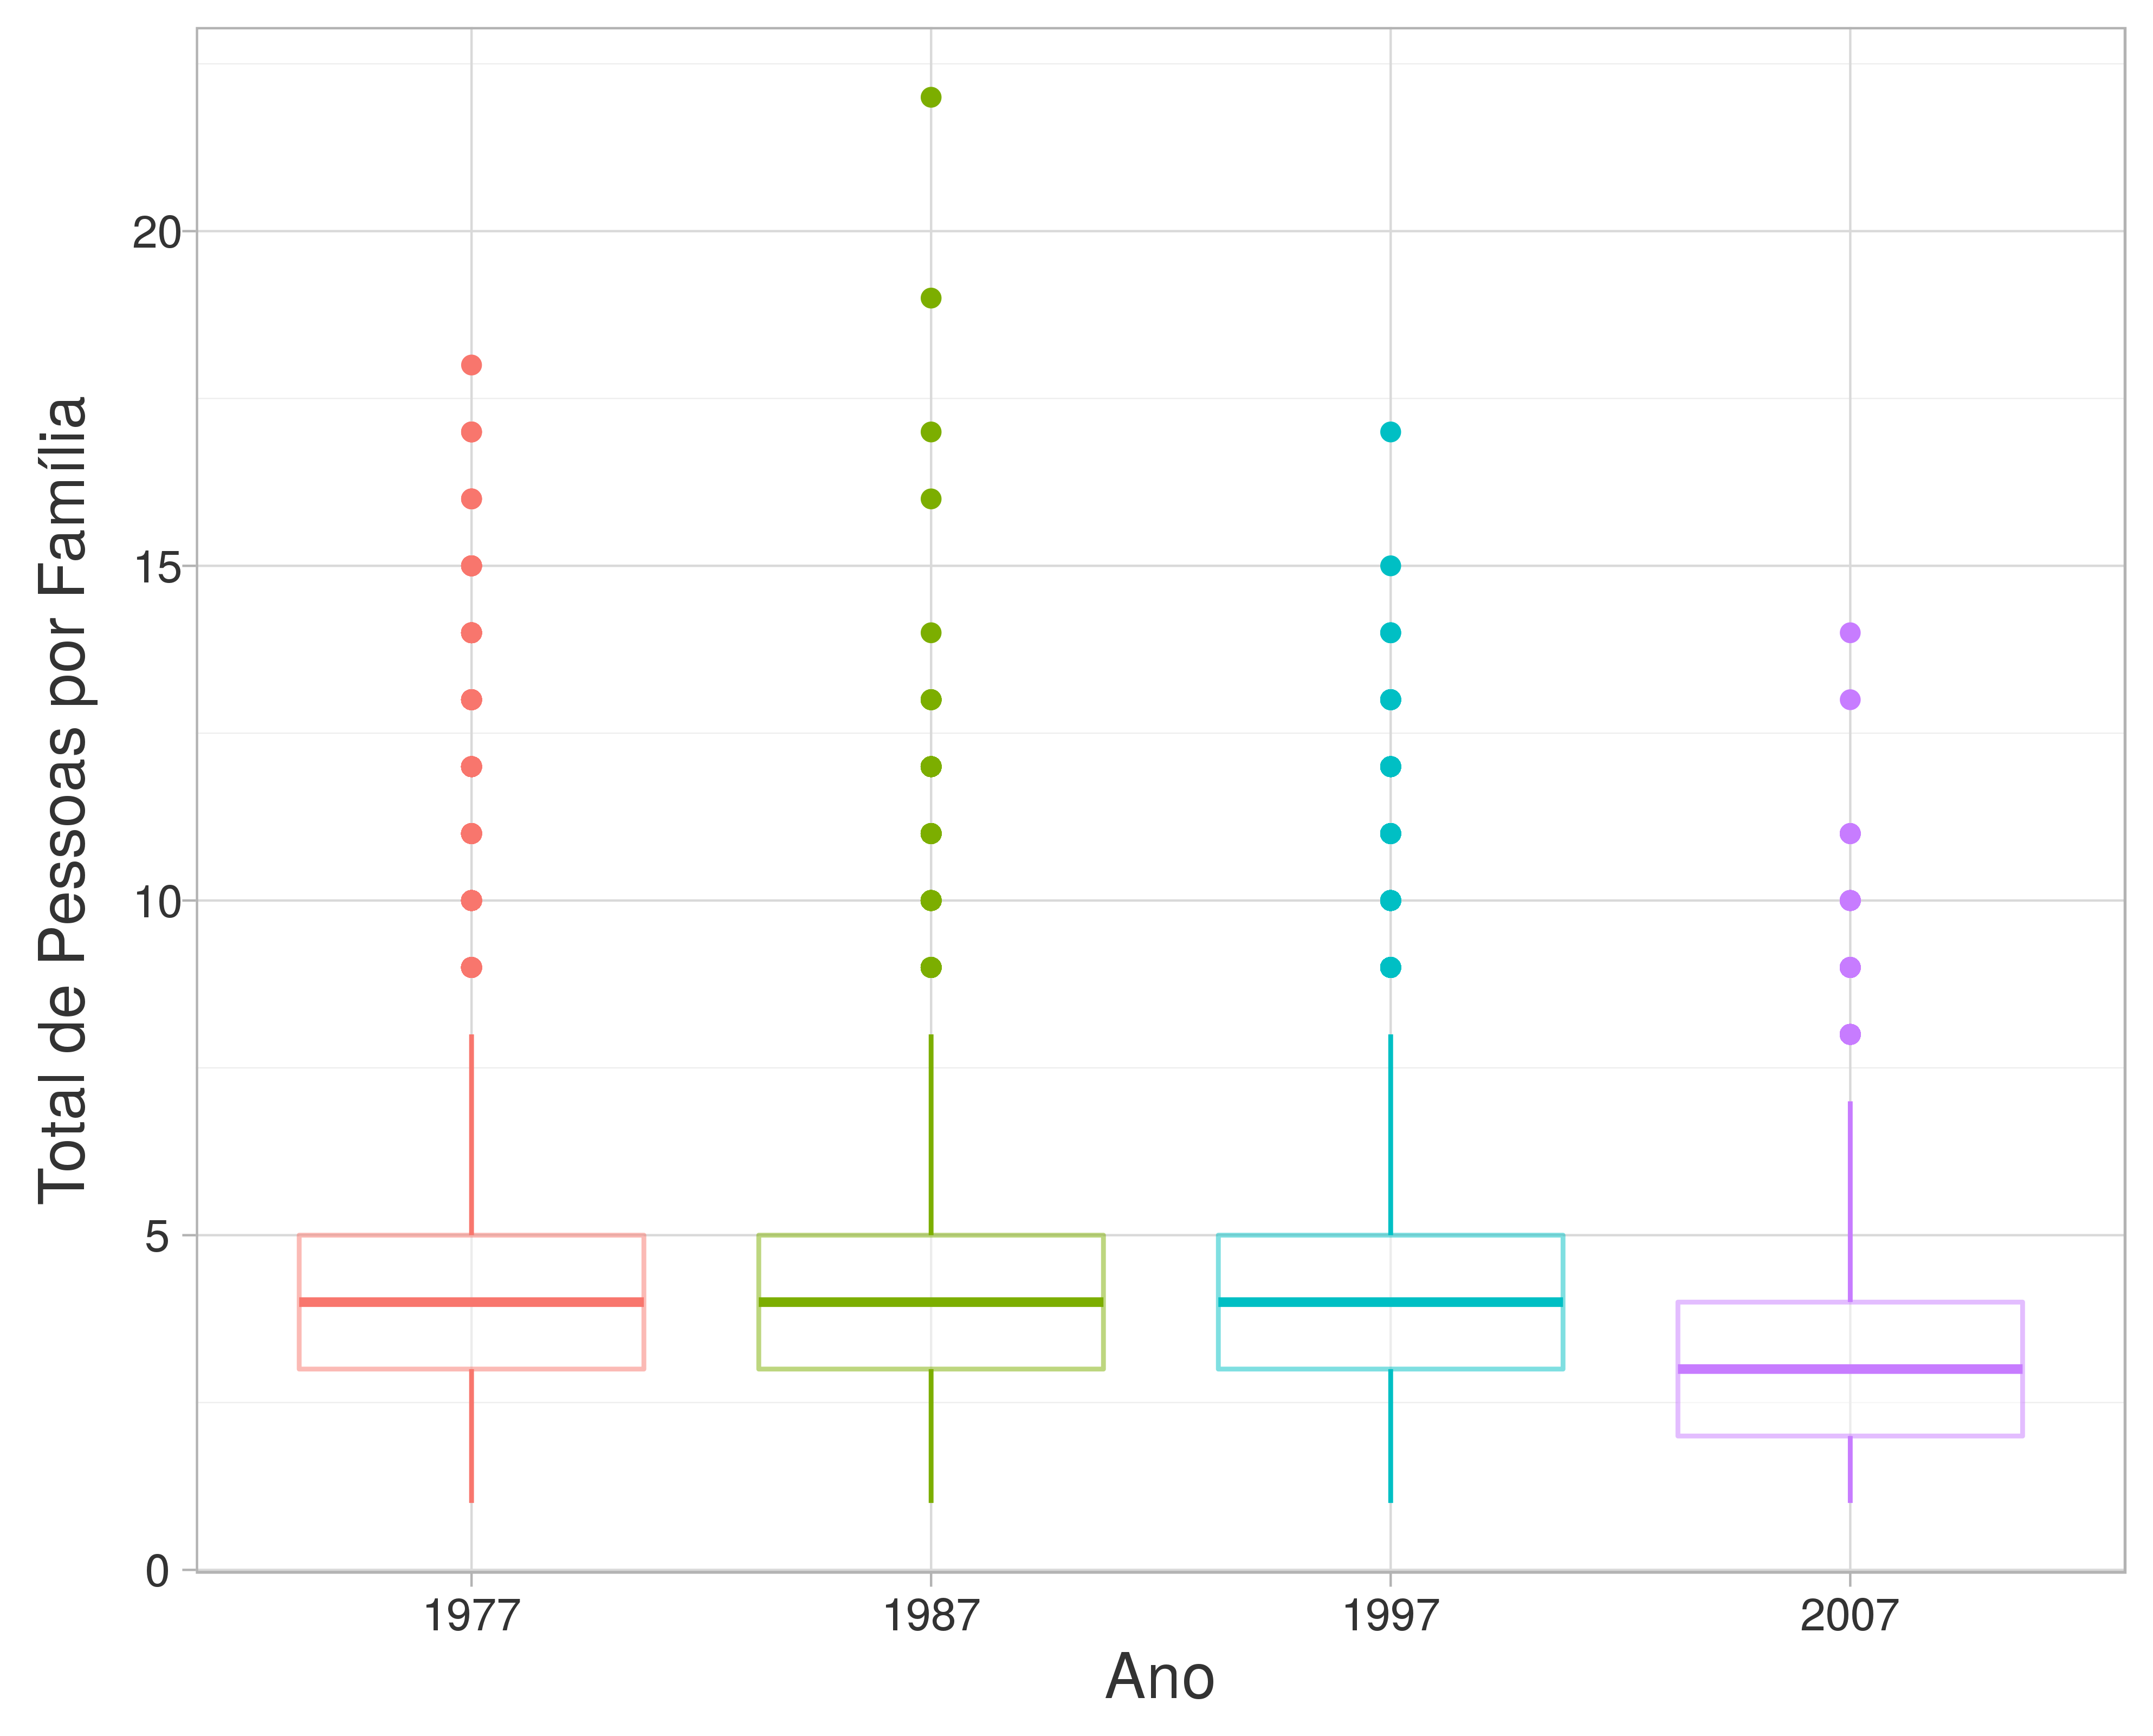
\includegraphics[width=1\textwidth]{./imagens/box-plot-tot-pess.png}%
    \end{center}%
    %\fonte{Compilação própria}
\end{figure}%

\newpage
Percebe-se pelo Gráfico \ref{graf:pres-flh-idoso-fam} a tendência de diminuição geral nas porcentagens de famílias com filhos pequenos (até 9 anos) a partir de 1987, efeito que será percebido na faixa etária seguinte (entre 10 e 19 anos) em 1997. Essa diminuição da presença de dependentes jovens (crianças/adolescentes) mantém-se em 2007. Nos mesmos períodos de análise, ocorre o envelhecimento da população, efeito capturado no gráfico pela presença de idosos (acima de 60 ou de 70 anos) com taxas positivas de crescimento.

\begin{grafico}[htb]%
    \caption{\label{graf:pres-flh-idoso-fam}Proporção de famílias com presença de dependentes, por ano}%
    \begin{center}%
        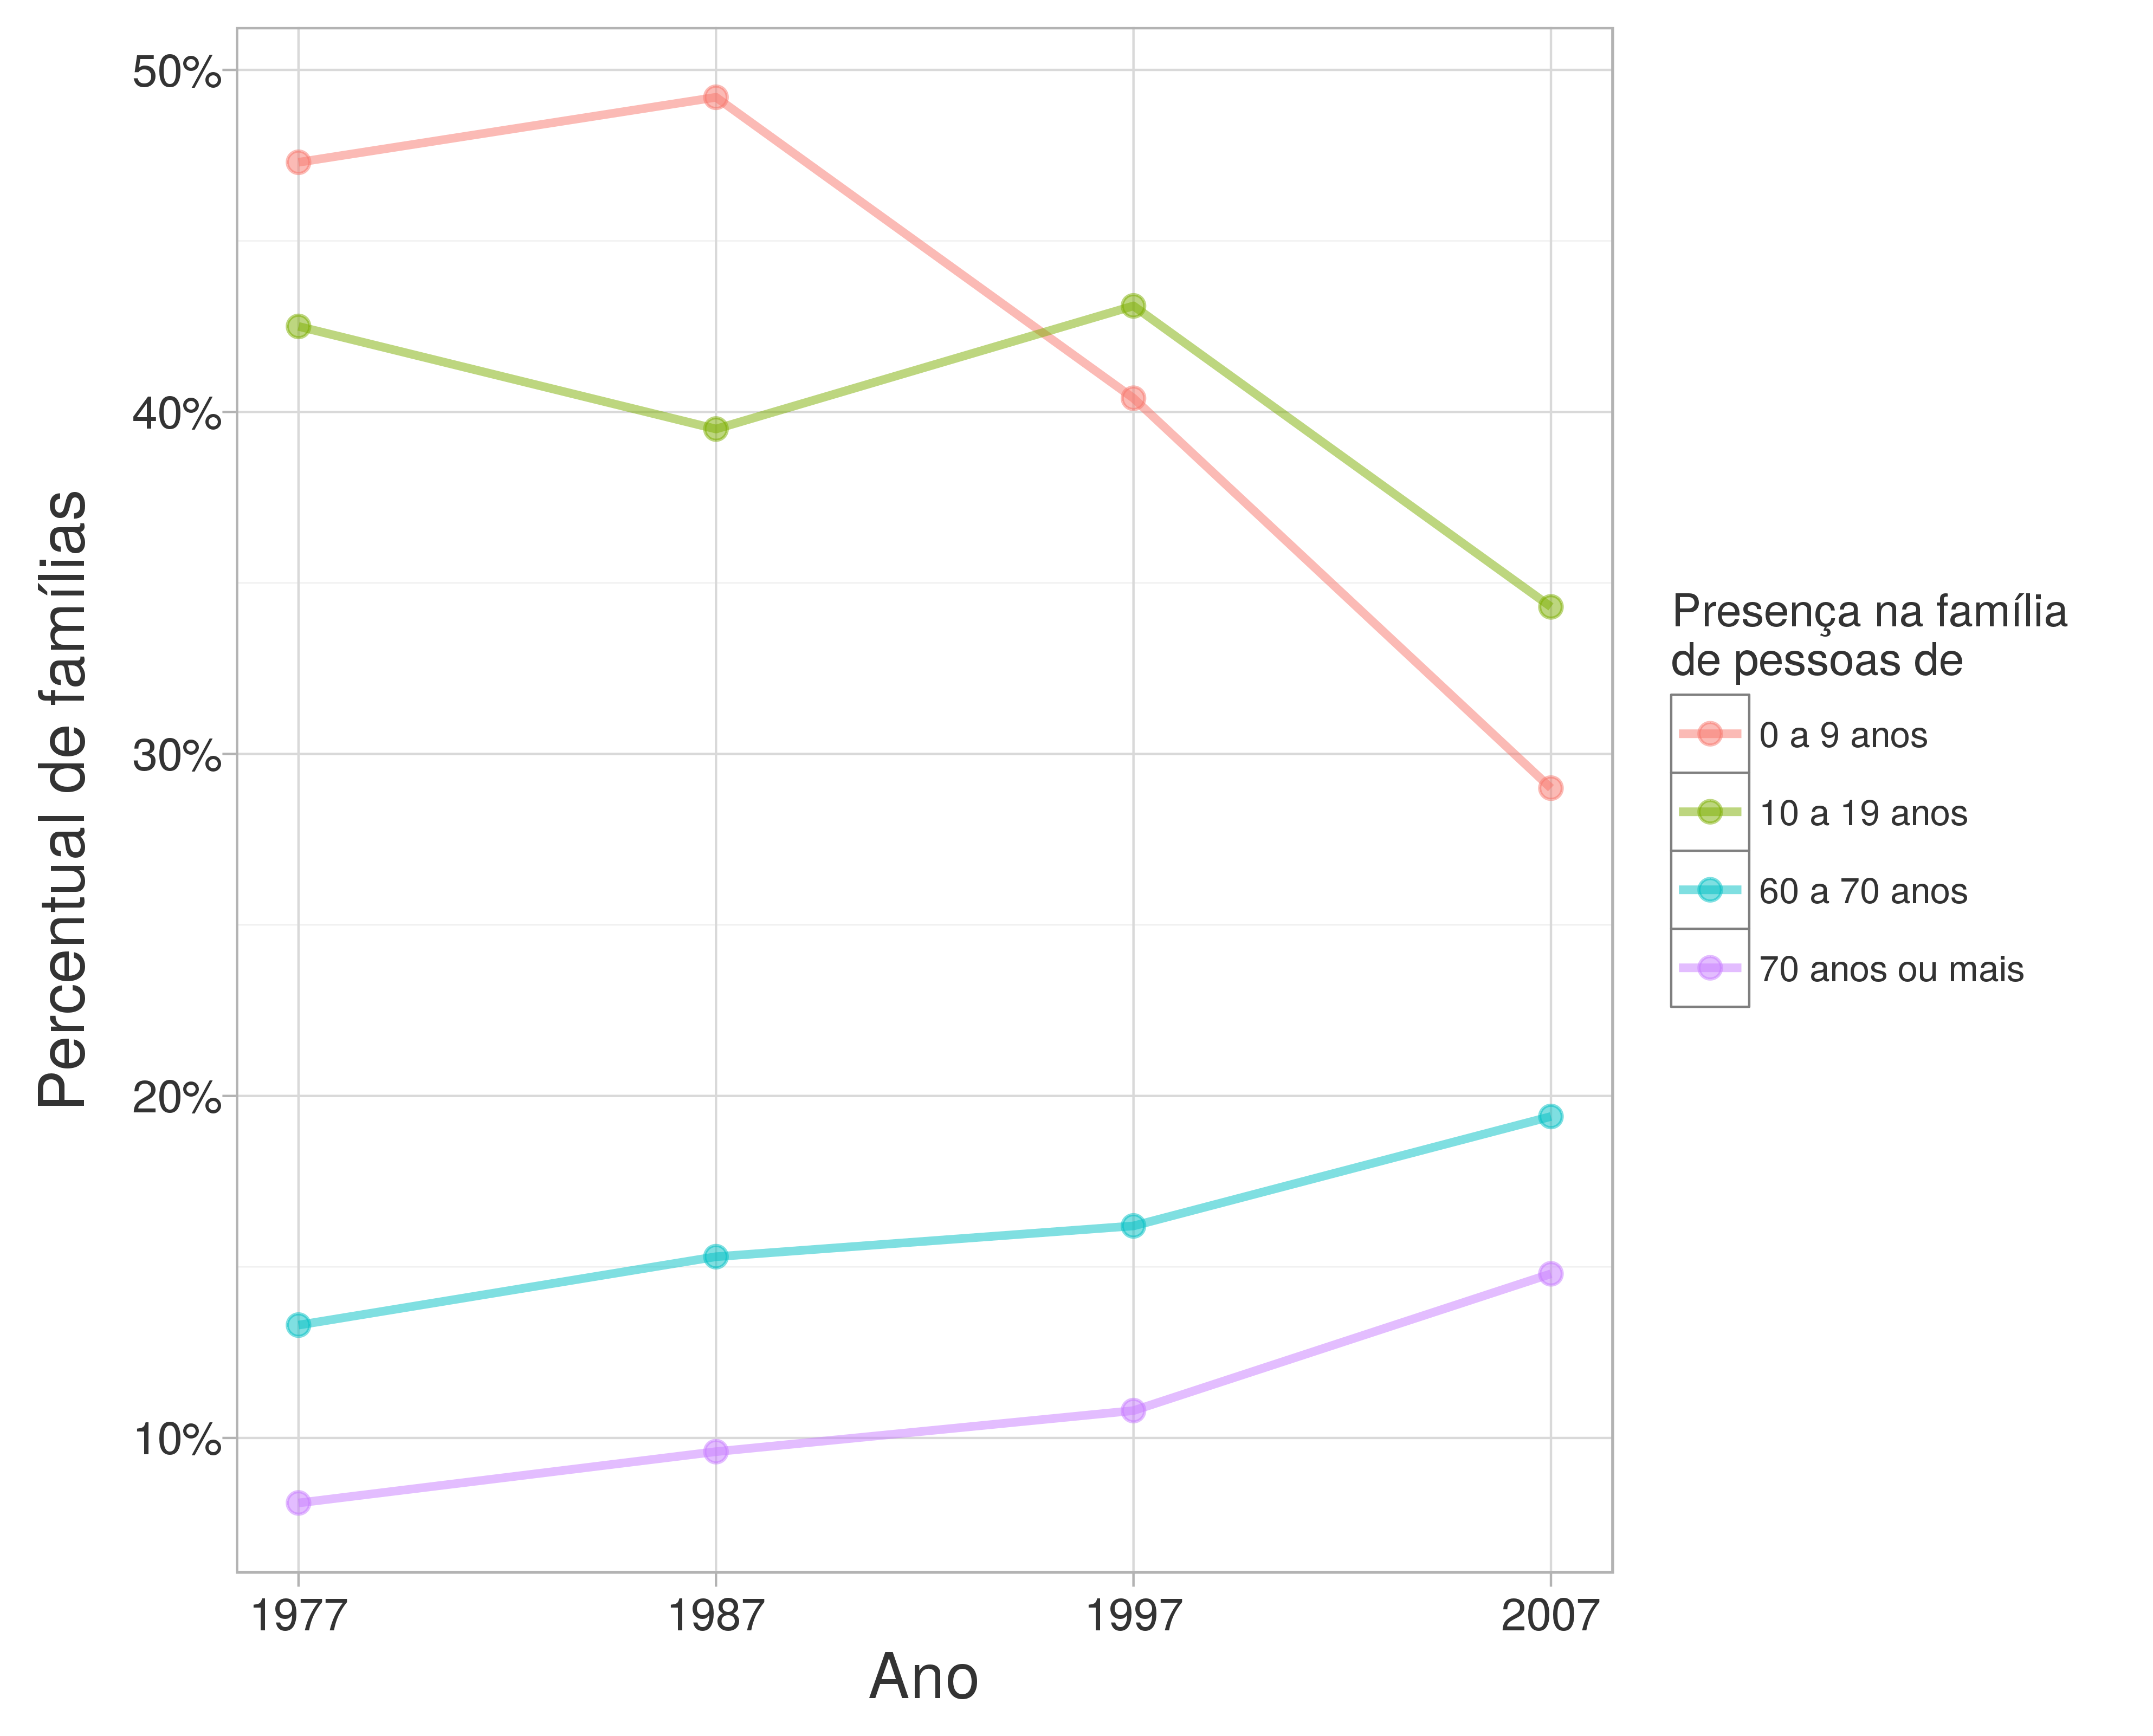
\includegraphics[width=1\textwidth]{./imagens/pres-flh-idoso-fam.png}%
    \end{center}%
    %\fonte{Compilação própria}
\end{grafico}%

Um dos fatores do indivíduo que influencia seu padrão de deslocamentos é o estágio no ``ciclo de vida'' \cite{BILT1997}.
Isto é, as atividades desenvolvidas por uma pessoa dependem em que fase da vida ela, e também os demais membros da família, se encontram. A variável \textbf{IDADE} é uma das variáveis que definem o ciclo de vida das pessoas. É possível perceber no Gráfico \ref{graf:distr-idade} que houve uma transição da pirâmide etária da RMSP, indicando envelhecimento da população tanto masculina como feminina.

\begin{grafico}[htb]%
    \caption{\label{graf:distr-idade}Distribuição da variável ``IDADE'' de respondentes, por ano e por sexo}%
    \begin{center}%
        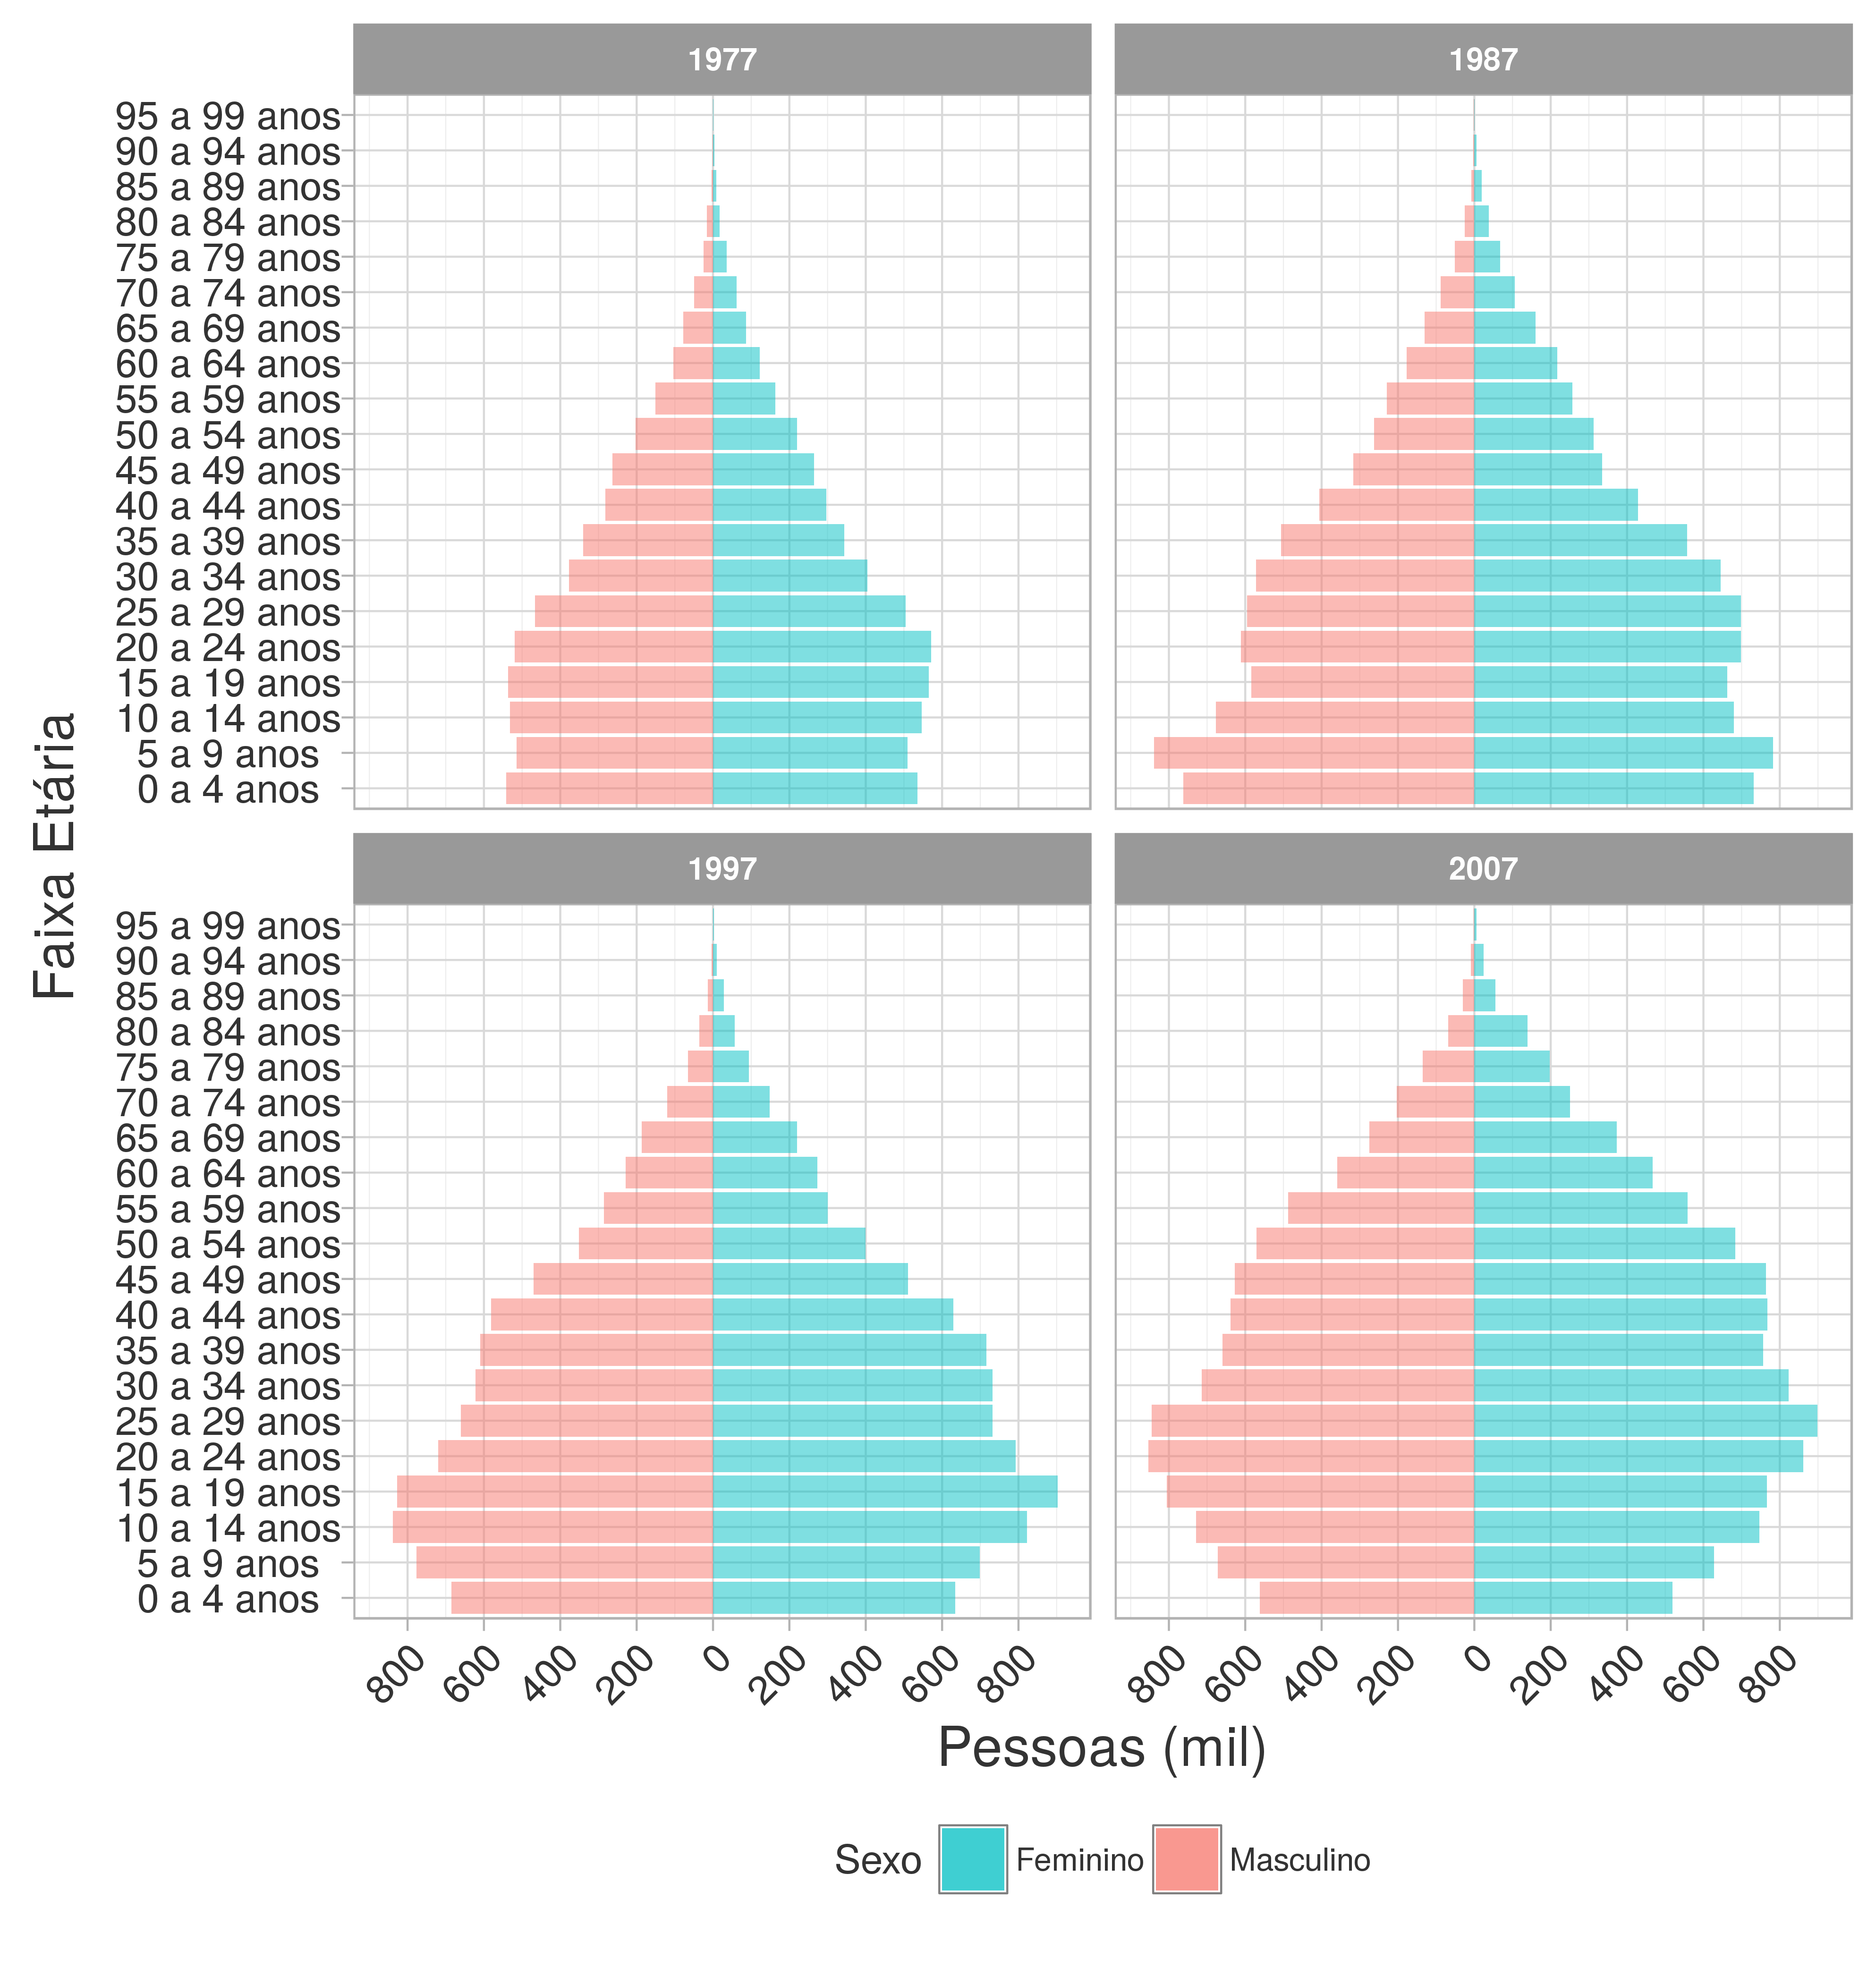
\includegraphics[width=1\textwidth]{./imagens/idade.png}%
    \end{center}%
%    \fonte{Compilação própria}
\end{grafico}%

Embora não exista relação identitária entre sexo e gênero, conforme já exposto na revisão de literatura, a variável \textbf{SEXO} é uma componente importante para compreender a categoria de análise gênero. Percebe-se na Tabela \ref{tab:prop-sexo} que em todos os anos a proporção de mulheres entrevistadas é superior à de homens, provavelmente devido ao fato de a pesquisa ser domiciliar e ser mais provável encontrar mulheres do que homens em casa.

\begin{table}[htb]
    \IBGEtab{%\renewcommand{\arraystretch}{1.5}%%\ABNTEXfontereduzida%
        \renewcommand{\arraystretch}{1.5}
        \caption{Frequências absoluta e relativa da variável SEXO, por ano}
        \label{tab:prop-sexo}
    }{%

    \begin{tabular}{ccccc}
        \toprule
        \textbf{ANO} & \textbf{1977} & \textbf{1987} & \textbf{1997} & \textbf{2007}\\ \midrule \midrule
        \textbf{\ quantidade de pessoas do sexo masculino na amostra} & 52.162 & 53.176 & 47.326 & 42.289 \\ \midrule
        \textbf{\% de pessoas do sexo masculino} & 48,3 & 48,0 & 47,9 & 46,3  \\ \midrule
%        \textbf{\% de pessoas do sexo masculino expandido} & 48,7 & 48,0 & 48,1 & 47,3  \\ \midrule        
        \textbf{\ quantidade de pessoas do sexo feminino na amostra} & 55.866 & 57.637 & 51.454 & 49.116  \\ \midrule
        \textbf{\% de pessoas do sexo feminino}  & 51,7 & 52,0 & 52,1 & 53,7  \\ \bottomrule
%        \textbf{\% de pessoas do sexo feminino expandido}  & 51,3 & 52,0 & 51,9 & 52,7 \\ \bottomrule
        \end{tabular}
    }

\end{table}
% Estatísticas para registros com F_PESS==1

\clearpage
Observando a variável situação familiar (\textbf{SIT_FAM}), nota-se que para as mulheres houve uma mudança ao longo dessas três décadas - ver Gráfico \ref{graf:distr-sit-fam}.
Em 1977, era mais frequente elas ocuparem a posição de filhas (41,8\%), em seguida de cônjuges (36,3\%).
A posição de ``pessoa responsável'' pela família é a quarta categoria mais frequente (6,3\%), de seis.
Tal distribuição permanece semelhante em 1987.
Em 1997, no entanto, a posição de ``pessoa responsável'' pela família (11,1\%) já quase se equipara à posição de ``outro parente/agregado(a)'' (11,3\%). Em 2007, se aproxima de um quarto proporção das mulheres entrevistadas que são responsáveis por suas famílias (22,6\%), representando aumento de mais de 3,5 vezes em relação aos percentuais de 1977. O percentual de mulheres cônjuges/companheiras pouco se altera ao longo do tempo, permanecendo na faixa dos 35\%. Há diminuição da posição de empregado(a) doméstico(a) para as mulheres (da ordem da metade). Existe, também, queda da frequência daqueles que se declaram na posição de filho(a) ou enteado(a) tanto para homens como para mulheres - em ordem de grandeza próxima: cerca de 10\% para mulheres e 9\% para homens. Isso pode ser reflexo da diminuição das taxas de fecundidade%
\footnote{Por ``taxa de fecundidade total'' entende-se o número médio de filhos que teria uma mulher de uma coorte hipotética (15 e 49 anos de idade) ao final de seu período reprodutivo. Fonte: IBGE. Disponível em: \url{http://www.ibge.gov.br/home/estatistica/populacao/condicaodevida/indicadoresminimos/conceitos.shtm\#tf}} 
da população (ver Tabela \ref{tab:taxa-fecund}). Entre os homens percebe-se que houve crescimento entre aqueles com posição de ``pessoas responsável'' de cerca de 3,5\%, e também dos que declaram-se cônjuge/companheiro (cerca de 20 vezes) - esta última constatação é coerente com o fato de mais mulheres serem a principal fonte de renda doméstica, ou seja, serem consideradas a ``pessoa responsável'' da família.

\begin{table}[htb]
    \IBGEtab{%\renewcommand{\arraystretch}{1.5}%%\ABNTEXfontereduzida%
	    \renewcommand{\arraystretch}{1.5}
        \caption{Evolução das taxas de fecundidade no Brasil, de 1970 a 2010}
		\label{tab:taxa-fecund}
    }{%
	    \begin{tabular}{P{5.00cm} P{1.50cm} P{1.50cm} P{1.50cm} P{1.50cm} P{1.50cm}}
            \toprule
	           \headerTabCenterCell{Ano} &
   	           \headerTabCenterCell{1970} &
   	           \headerTabCenterCell{1980} &
   	           \headerTabCenterCell{1991} &
   	           \headerTabCenterCell{2000} &
   	           \headerTabCenterCell{2010} \\
		    \midrule \midrule
				Taxa de fecundidade (Brasil)&
				5,8&
				4,4&
				2,7&
				2,4&
		        1,9\\
			\midrule
				Taxa de fecundidade (Sudeste)&
				4,6&
				3,2&
				2,4&
				2,1&
		        1,7\\
			\midrule
				Taxa de fecundidade (São Paulo)&
				3,94&
				3,24&
				2,28&
				2,05&
		        1,67\\
			\bottomrule	
		\end{tabular}
    }{%
		\fonte{Compilação a partir de dados dos censos do IBGE disponíveis em \url{http://seculoxx.ibge.gov.br/populacionais-sociais-politicas-e-culturais/busca-por-palavra-chave/populacao/810-fecundidade} Acesso em 17 de novembro de 2014}
		\nota{Ao analisar as taxas de fecundidades para as Grandes Regiões, nota-se que o Sudeste tem os menores percentuais de mulheres que tiveram filhos em todos os subgrupos etários.}
		}
\end{table}

Tem-se como uma das hipótese deste trabalho que houve evolução dos padrões de mobilidade por gênero.
Articular as variáveis sexo e situação familiar pode ser uma estratégia para tentar utilizar o gênero como categoria de análise.

\begin{grafico}[htb]%
    \caption{\label{graf:distr-sit-fam}Distribuição da variável ``SIT_FAM'', por ano e por sexo}%
    \begin{center}%
        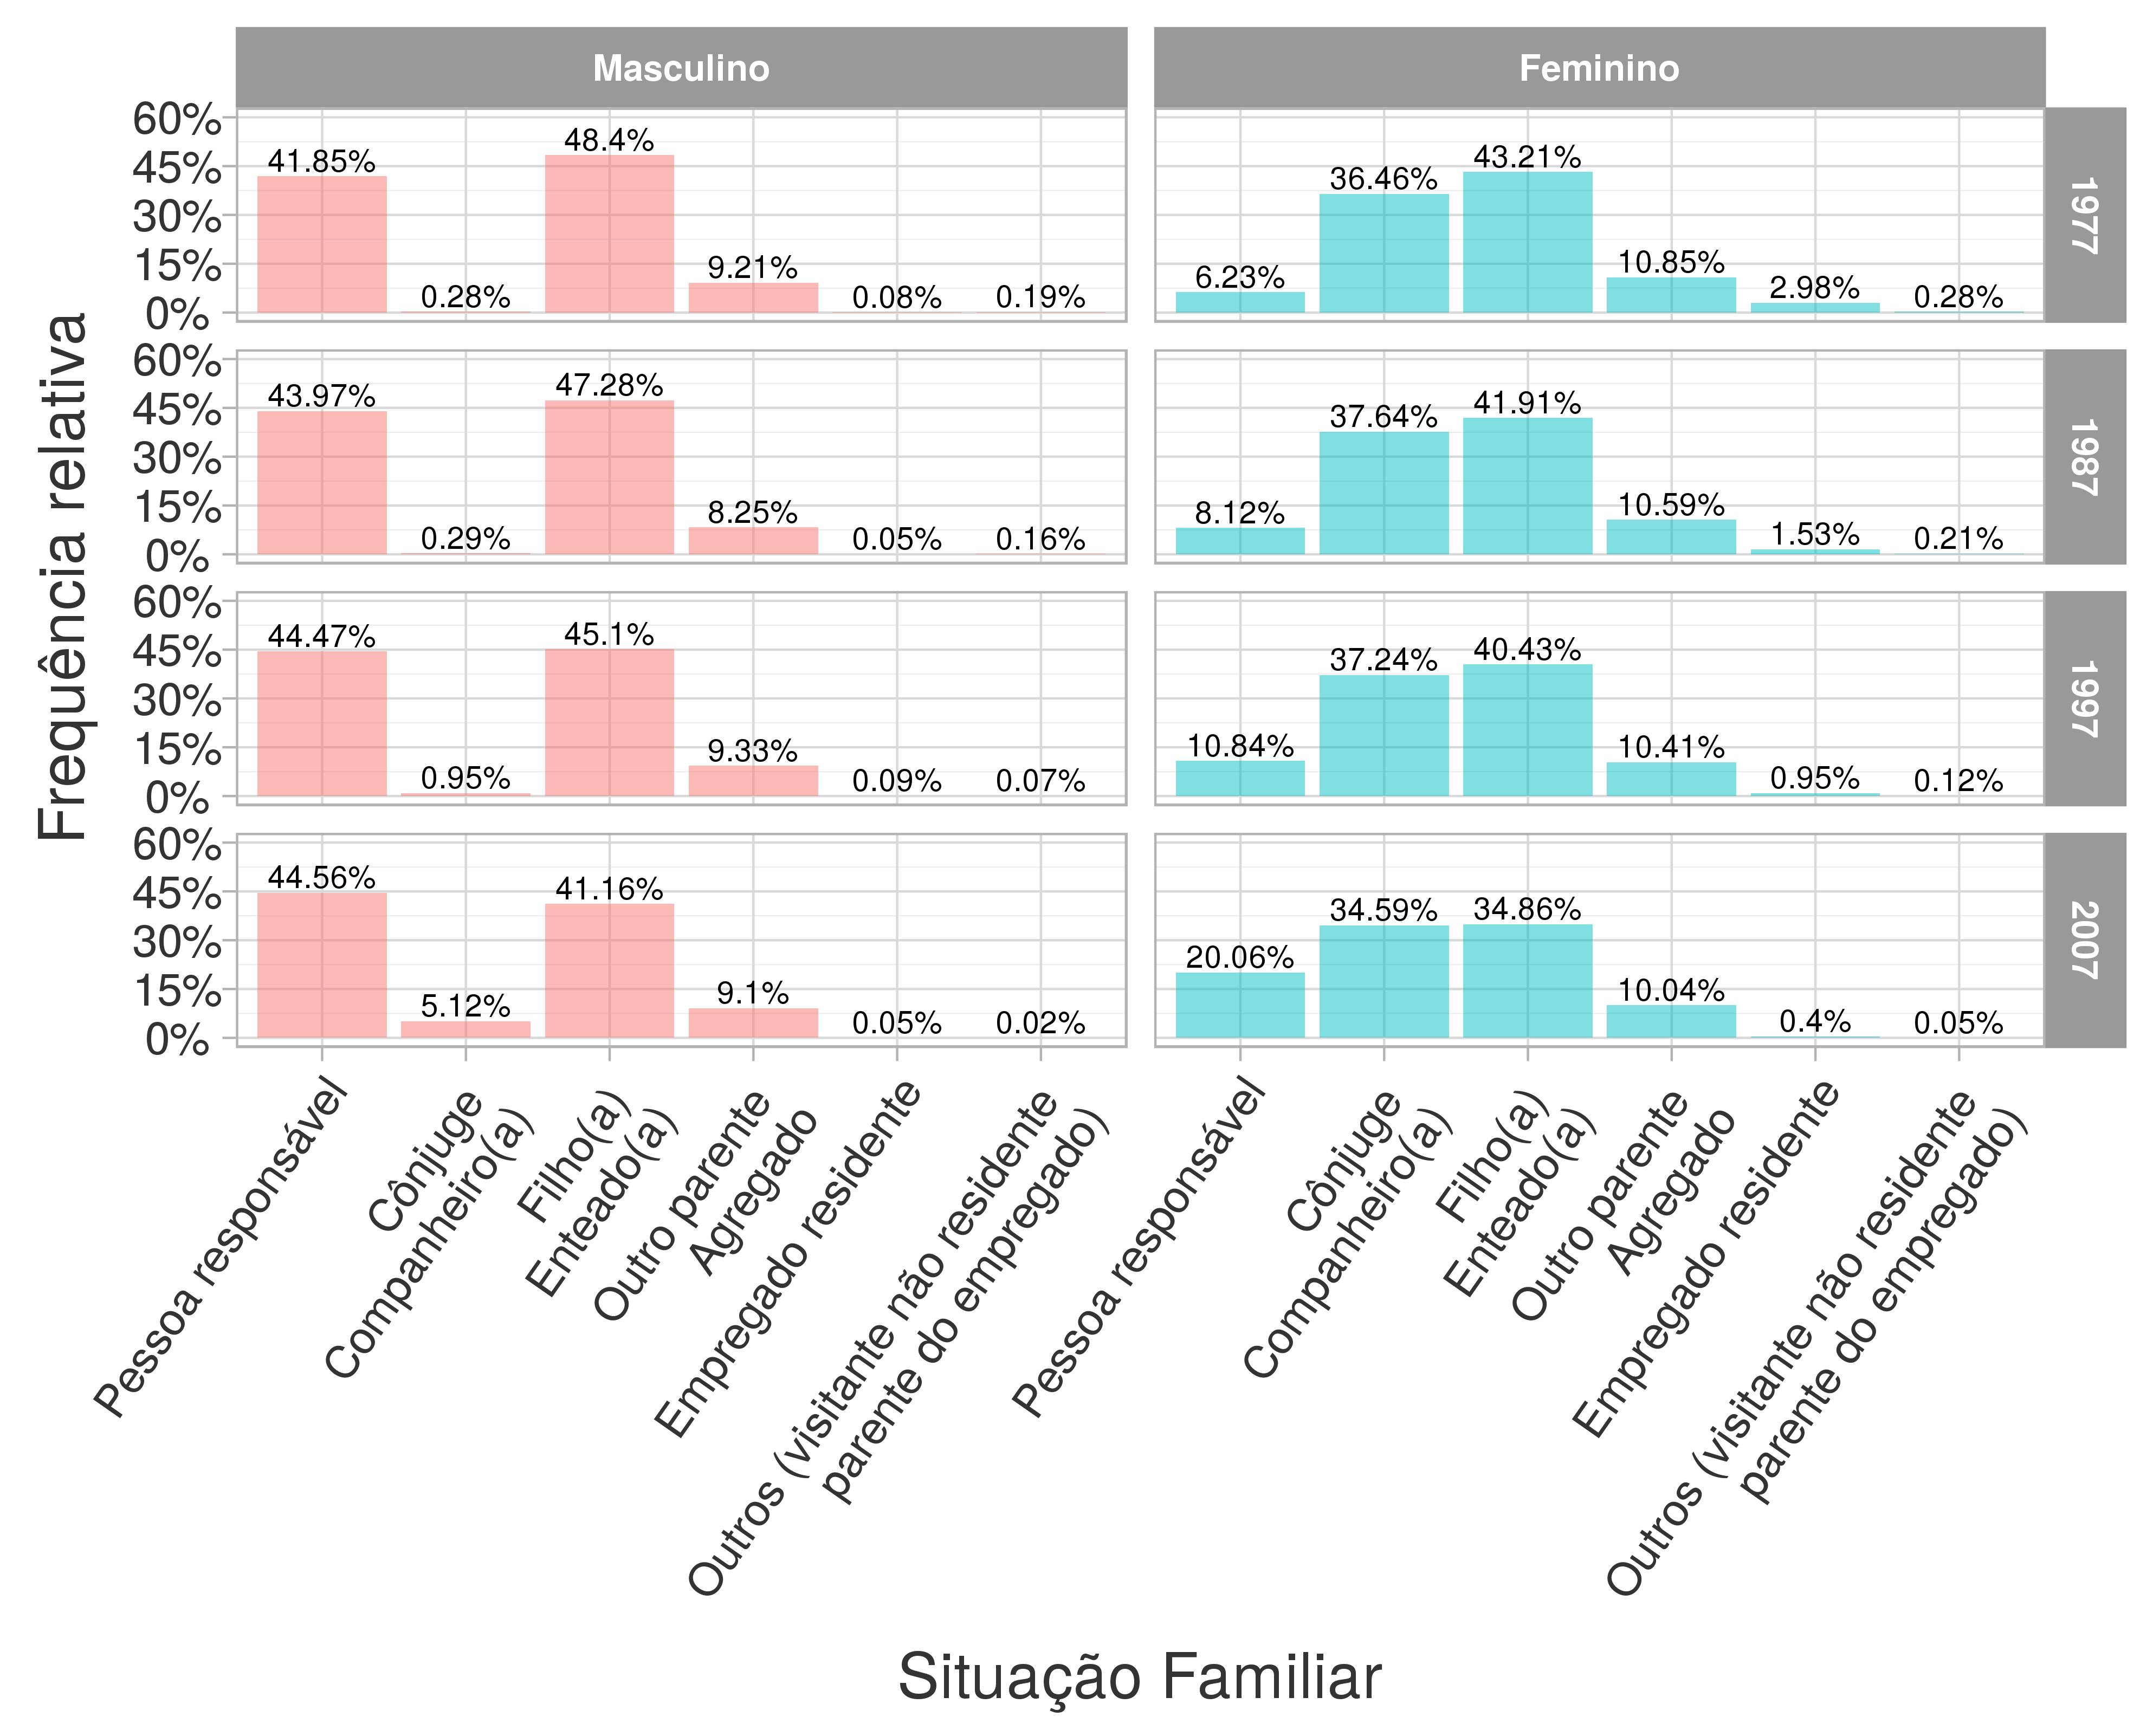
\includegraphics[width=1\textwidth]{./imagens/sit-fam.png}%
    \end{center}%
%    \fonte{Compilação própria}
\end{grafico}%

\citeauthoronline{BILT1997} (\citeyear{BILT1997}), a partir da análise de trabalhos de diversos autores, para compreender melhor o comportamento das pessoas em relação à participação em atividades e a consequente geração de viagens, 
elenca como conceito importante, além do estágio no ciclo de vida familiar e dos papéis sociais, o estilo de vida.
Duas das variáveis que auxiliam a caracterizar o estilo de vida da pessoa respondente é saber se ela estuda e se ela trabalha.

A variável \textbf{TRABALHA} foi construída a partir da variável OCUP da seguinte maneira: se a categoria da ocupação fosse 1, correspondente a ``tem trabalho'', a variável recebia valor 1, caso contrário, recebia valor 0.
A variável \textbf{ESTUDA} conta com as categorias sim (1) e não (0). Em 1987, 1997 e 2007 esta variável existe, mas somente com a categoria ``não'' em comum. Assim, as demais alternativas de resposta tornaram-se simplesmente ``sim'', independente das subdivisões que apresentassem. Para 1977, ano em que essa variável não existe, ela foi preenchida segundo o seguinte critério: a pessoa foi considerada estudante se o campo ``Zona da escola'' dela não fosse vazio ou igual a zero. Preferiu-se não utilizar a categoria ``estudante'' da variável ocupação para não perder a informação de quem estuda e trabalha, pois neste caso, estudante não seria a ocupação principal da pessoa e sim ``tem trabalho''.

% Fazendo o seguinte:
% od %>% filter(SERV_PAS_DEST==1, ZONA_DEST==ZONA_ESC, SUBZONA_DEST==SUBZONA_ESC, ANO==1) %>% select(ESTUDA, ID_PESS) %>% count(ID_PESS)
% Obtive: 72 pessoas que podem ter sido registrados erroneamnte domo estudantes em 1977

As Tabelas \ref{tab:prop-trabalha} e \ref{tab:prop-estuda} indicam as frequências das \textit{dummies} TRABALHA e ESTUDA, por ano e por sexo, em relação à população (aplicados os fatores de expansão).
Percebe-se que o percentual de trabalhadores(as) aumenta na população devido à maior participação feminina no mercado de trabalho, dado que os percentuais dos trabalhadores permanecem no mesmo patamar (24\% da população). Segmentando por sexo, vê-se que houve um aumento de quase 20\% na participação feminina no mercado de trabalho e pouco mais de 2\% de incremento na masculina.
Analisando as proporções de mulheres e homens estudantes, nota-que que houve pequeno crescimento entre 1977 e 1997 (3,2\% feminino e 2,5\% masculino) seguido de leve queda (1,5\% pra ambos sexos). A expectativa era de ter havido um grande crescimento percentual do número de estudantes, especialmente mulheres, para o período observado. O crescimento tímido pode dever-se ao fato de que, embora a população da RMSP tenha elevado seus níveis de escolarização, o crescimento (desacelerando) e o envelhecimento (em ascensão) da população implicam haver mais gente fora da faixa etária escolar do que dentro dela. As quedas no percentual de estudantes pode estar relacionada tanto ao envelhecimento da população quanto à saturação do sistema de ensino, cuja obrigatoriedade de oferta pública limita-se à Educação Básica (9 anos de Ensino Fundamental e 3 anos de Ensino Médio). 


\begin{table}[htb]
    \IBGEtab{%\renewcommand{\arraystretch}{1.5}%%\ABNTEXfontereduzida%
        \renewcommand{\arraystretch}{1.5}
        \caption{Frequências da variável TRABALHA, por ano e sexo}
        \label{tab:prop-trabalha}
    }{%

    \begin{tabular}{ccccc}
        \toprule
        \textbf{ANO} & \textbf{1977} & \textbf{1987} & \textbf{1997} & \textbf{2007}\\ \midrule \midrule
        \textbf{\% de trabalhadoras relativo ao total da população} & 9,78 & 12,18 & 16,27 & 19,88  \\ \midrule
        \textbf{\% de trabalhadores relativo ao total da população} & 24,42 & 24,73 & 24,61 & 24,82  \\ \midrule
        \textbf{\% de trabalhadoras relativo ao total de mulheres} & 19,08 & 23,44 & 31,38 & 37,76  \\ \midrule
        \textbf{\% de trabalhadores relativo ao total de homens} & 50,12 & 51,50 & 51,13 & 52,42  \\ \midrule
        \textbf{\% de trabalhadores(as) relativo ao total da população} & 34,20 & 36,91 & 40,89 & 44,70  \\ \bottomrule
        \end{tabular}
    }

\end{table}
% Estatísticas para registros com F_PESS==1

%No campo OCUP (35) as classificações de cada ano são bastante diferentes. Assim, decidiu-se por discriminar quem não respondeu, quem é estudante, quem é dono(a) de casa, que é aposentado(a), quem não tem ocupação (como por exemplo, crianças), quem está desempregado(a), quem está em licença e quem trabalha (em todas opções possíveis dadas em todas as Pesquisas OD).
%
%\begin{table}[htb]
%    \IBGEtab{%\renewcommand{\arraystretch}{1.5}%%\ABNTEXfontereduzida%
%        \renewcommand{\arraystretch}{1.5}
%        \caption{Estatísticas da variável ``OCUP''}
%        \label{tab:estat-ocup}
%    }{%
%
%    \begin{tabular}{cccccc}
%        \toprule
%        \textbf{ANO} & \textbf{1977} & \textbf{1987} & \textbf{1997} & \textbf{2007} & \textbf{Total}\\ \midrule \midrule
%        \textbf{OCUP=1}  &  3.666 & 41.082 & 41.474 & 43.838 & 163.060 \\ \hline
%        \textbf{OCUP=2}  &    736 &    668 &    447 &    574 &   2.425 \\ \hline
%        \textbf{OCUP=3}  &  3.869 &  6.664 &  7.553 & 13.125 &  31.211 \\ \hline
%        \textbf{OCUP=4}  &  2.256 &  3.304 &  6.297 &  6.500 &  18.357 \\ \hline
%        \textbf{OCUP=5}  & 16.519 & 17.118 &  8.604 &  6.717 &  48.958 \\ \hline
%        \textbf{OCUP=6}  & 22.571 & 20.283 & 11.484 &  7.082 &  61.420 \\ \hline
%        \textbf{OCUP=7}  & 20.415 & 21.409 & 22.921 & 13.569 &  78.314 \\ \hline
%        \textbf{OCUP=NA} &  4.996 &    285 &      0 &      0 &   5.281 \\ \bottomrule
%        \end{tabular}
%    }
%
%\end{table}
%% Estatísticas para registros com F_PESS==1
%
%No campo SETOR_ATIV (36), nos anos em que há opção de indicar o setor de mais de um trabalho (caso a pessoa tenha mais de um trabalho), foi considerado o setor do primeiro trabalho.
%
%\begin{table}[htb]
%    \IBGEtab{%\renewcommand{\arraystretch}{1.5}%%\ABNTEXfontereduzida%
%        \renewcommand{\arraystretch}{1.5}
%        \caption{Estatísticas da variável ``SETOR_ATIV''}
%        \label{tab:estat-setor-ativ}
%    }{%
%
%    \begin{tabular}{cccccc}
%        \toprule
%        \textbf{ANO} & \textbf{1977} & \textbf{1987} & \textbf{1997} & \textbf{2007} & \textbf{Total}\\ \midrule \midrule
%        \textbf{SETOR_ATIV=1}  &    252 &    252 &    394 &    163 &   1.061 \\ \hline
%        \textbf{SETOR_ATIV=2}  &  1.248 &  1.012 &  2.350 &  1.483 &   6.093 \\ \hline
%        \textbf{SETOR_ATIV=3}  & 12.381 & 12.391 &  6.002 &  4.676 &  35.450 \\ \hline
%        \textbf{SETOR_ATIV=4}  &  7.992 &  7.785 &  9.389 &  7.900 &  33.066 \\ \hline
%        \textbf{SETOR_ATIV=5}  &  3.336 &  3.745 &  1.693 &  1.544 &  10.318 \\ \hline
%        \textbf{SETOR_ATIV=6}  &    952 &  1.069 &  2.023 &  1.534 &   5.578 \\ \hline
%        \textbf{SETOR_ATIV=7}  & 13.618 & 16.948 & 10.522 & 15.353 &  56.441 \\ \hline
%        \textbf{SETOR_ATIV=8}  &    165 &    158 &  9.385 &      0 &   9.708 \\ \hline
%        \textbf{SETOR_ATIV=9}  & 63.086 & 67.171 & 57.022 & 12.130 & 199.409 \\ \hline
%        \textbf{SETOR_ATIV=NA} &  4.998 &    282 &      0 & 46.622 &  51.902 \\ \bottomrule
%        \end{tabular}
%    }
%
%\end{table}
%% Estatísticas para registros com F_PESS==1

\begin{table}[htb]
    \IBGEtab{%\renewcommand{\arraystretch}{1.5}%%\ABNTEXfontereduzida%
        \renewcommand{\arraystretch}{1.5}
        \caption{Frequências da variável ESTUDA, por ano e sexo}
        \label{tab:prop-estuda}
    }{%

    \begin{tabular}{ccccc}
        \toprule
        \textbf{ANO} & \textbf{1977} & \textbf{1987} & \textbf{1997} & \textbf{2007}\\ \midrule \midrule
        \textbf{\% de estudantes mulheres relativo ao total da população} & 11,94 & 12,88 & 15,17 & 13,75  \\ \midrule
        \textbf{\% de estudantes homens relativo ao total da população} & 12,55 & 12,92 & 14,99 & 13,42  \\ \midrule
        \textbf{\% de estudantes mulheres relativo ao total de mulheres} & 23,30 & 24,79 & 29,25 & 26,12  \\ \midrule
        \textbf{\% de estudantes homens relativo ao total de homens} & 25,74 & 26,90 & 31,15 & 28,35  \\ \midrule
        \textbf{\% de estudantes relativo ao total da população} & 24,49 & 25,80 & 30,17 & 27,18  \\ \bottomrule
        \end{tabular}
    }

\end{table}
% Estatísticas para registros com F_PESS==1

\newpage
No Gráfico \ref{graf:distr-grau-instr} nota-se que em 1977 tanto homens como mulheres dispunham de pouco tempo de escolaridade - mais de três quartos da população ou era analfabeta ou possuía no máximo o fundamental incompleto. Nessa época, nos três níveis de instrução superiores a esse os homens tinham índices maiores que as mulheres. O grau de instrução (\textbf{GRAU_INSTR}) da população vai aumentando e em 1987, o grau de escolarização feminino é levemente superior ao masculino nas categorias ``fundamental completo / médio incompleto'' e ``médio completo / superior incompleto''. Na categoria ``superior completo'' o grau de instrução masculino é um pouco superior, situação que se inverte em 2007. Neste último ano de análise, as mulheres apresentam maiores percentuais nos dois níveis de maior grau de instrução.

%Mesmo assim, as marcas para ambos são bastante semelhantes e indicam esforços de políticas públicas no sentido de universalizar os Ensinos Fundamental e Médio no Brasil \ref{tab:grau-instr-ef-em}.
%
%\begin{table}[htb]
%    \IBGEtab{%\renewcommand{\arraystretch}{1.5}%%\ABNTEXfontereduzida%
%	    \renewcommand{\arraystretch}{1.5}
%        \caption{Crescimento de matrículas no Ensino Fundamental e Ensino Médio, no Brasil, entre 1975 e 2005}
%		\label{tab:grau-instr-ef-em}
%    }{%
%	    \begin{tabular}{P{2.00cm} P{4.00cm} P{4.00cm}}
%            \toprule
%	           \headerTabCenterCell{Ano} &
%   	           \headerTabCenterCell{Matrículas no Ensino Fundamental} &
%   	           \headerTabCenterCell{Matrículas no Ensino Médio}\\
%		    \midrule \midrule
%				1975&
%		    	100*&
%				100*\\
%			\midrule
%				1980&
%				115,6&
%		        113,1\\
%			\midrule
%				1990&
%				141,0**&
%		        180,8\\
%			\midrule
%				1996&
%				169,5&
%		        296,4\\
%			\midrule
%				2000&
%				182,7&
%		        423,2\\
%			\midrule
%				2005&
%				171,5&
%		        466,5\\
%			\bottomrule	
%		\end{tabular}
%    }{%
%		\fonte{Adaptado de \citeauthoronline{OLIVEIRA2007} (\citeyear{OLIVEIRA2007})}
%		\nota{* Tomou-se por referência o ano de 1975 (1975=100). 
%		** O valor refere-se ao ano de 1989.}
%	}
%\end{table}

\begin{grafico}[htb]%
    \caption{\label{graf:distr-grau-instr} Distribuição da variável ``GRAU_INSTR'', por ano e por sexo}%
    \begin{center}%
        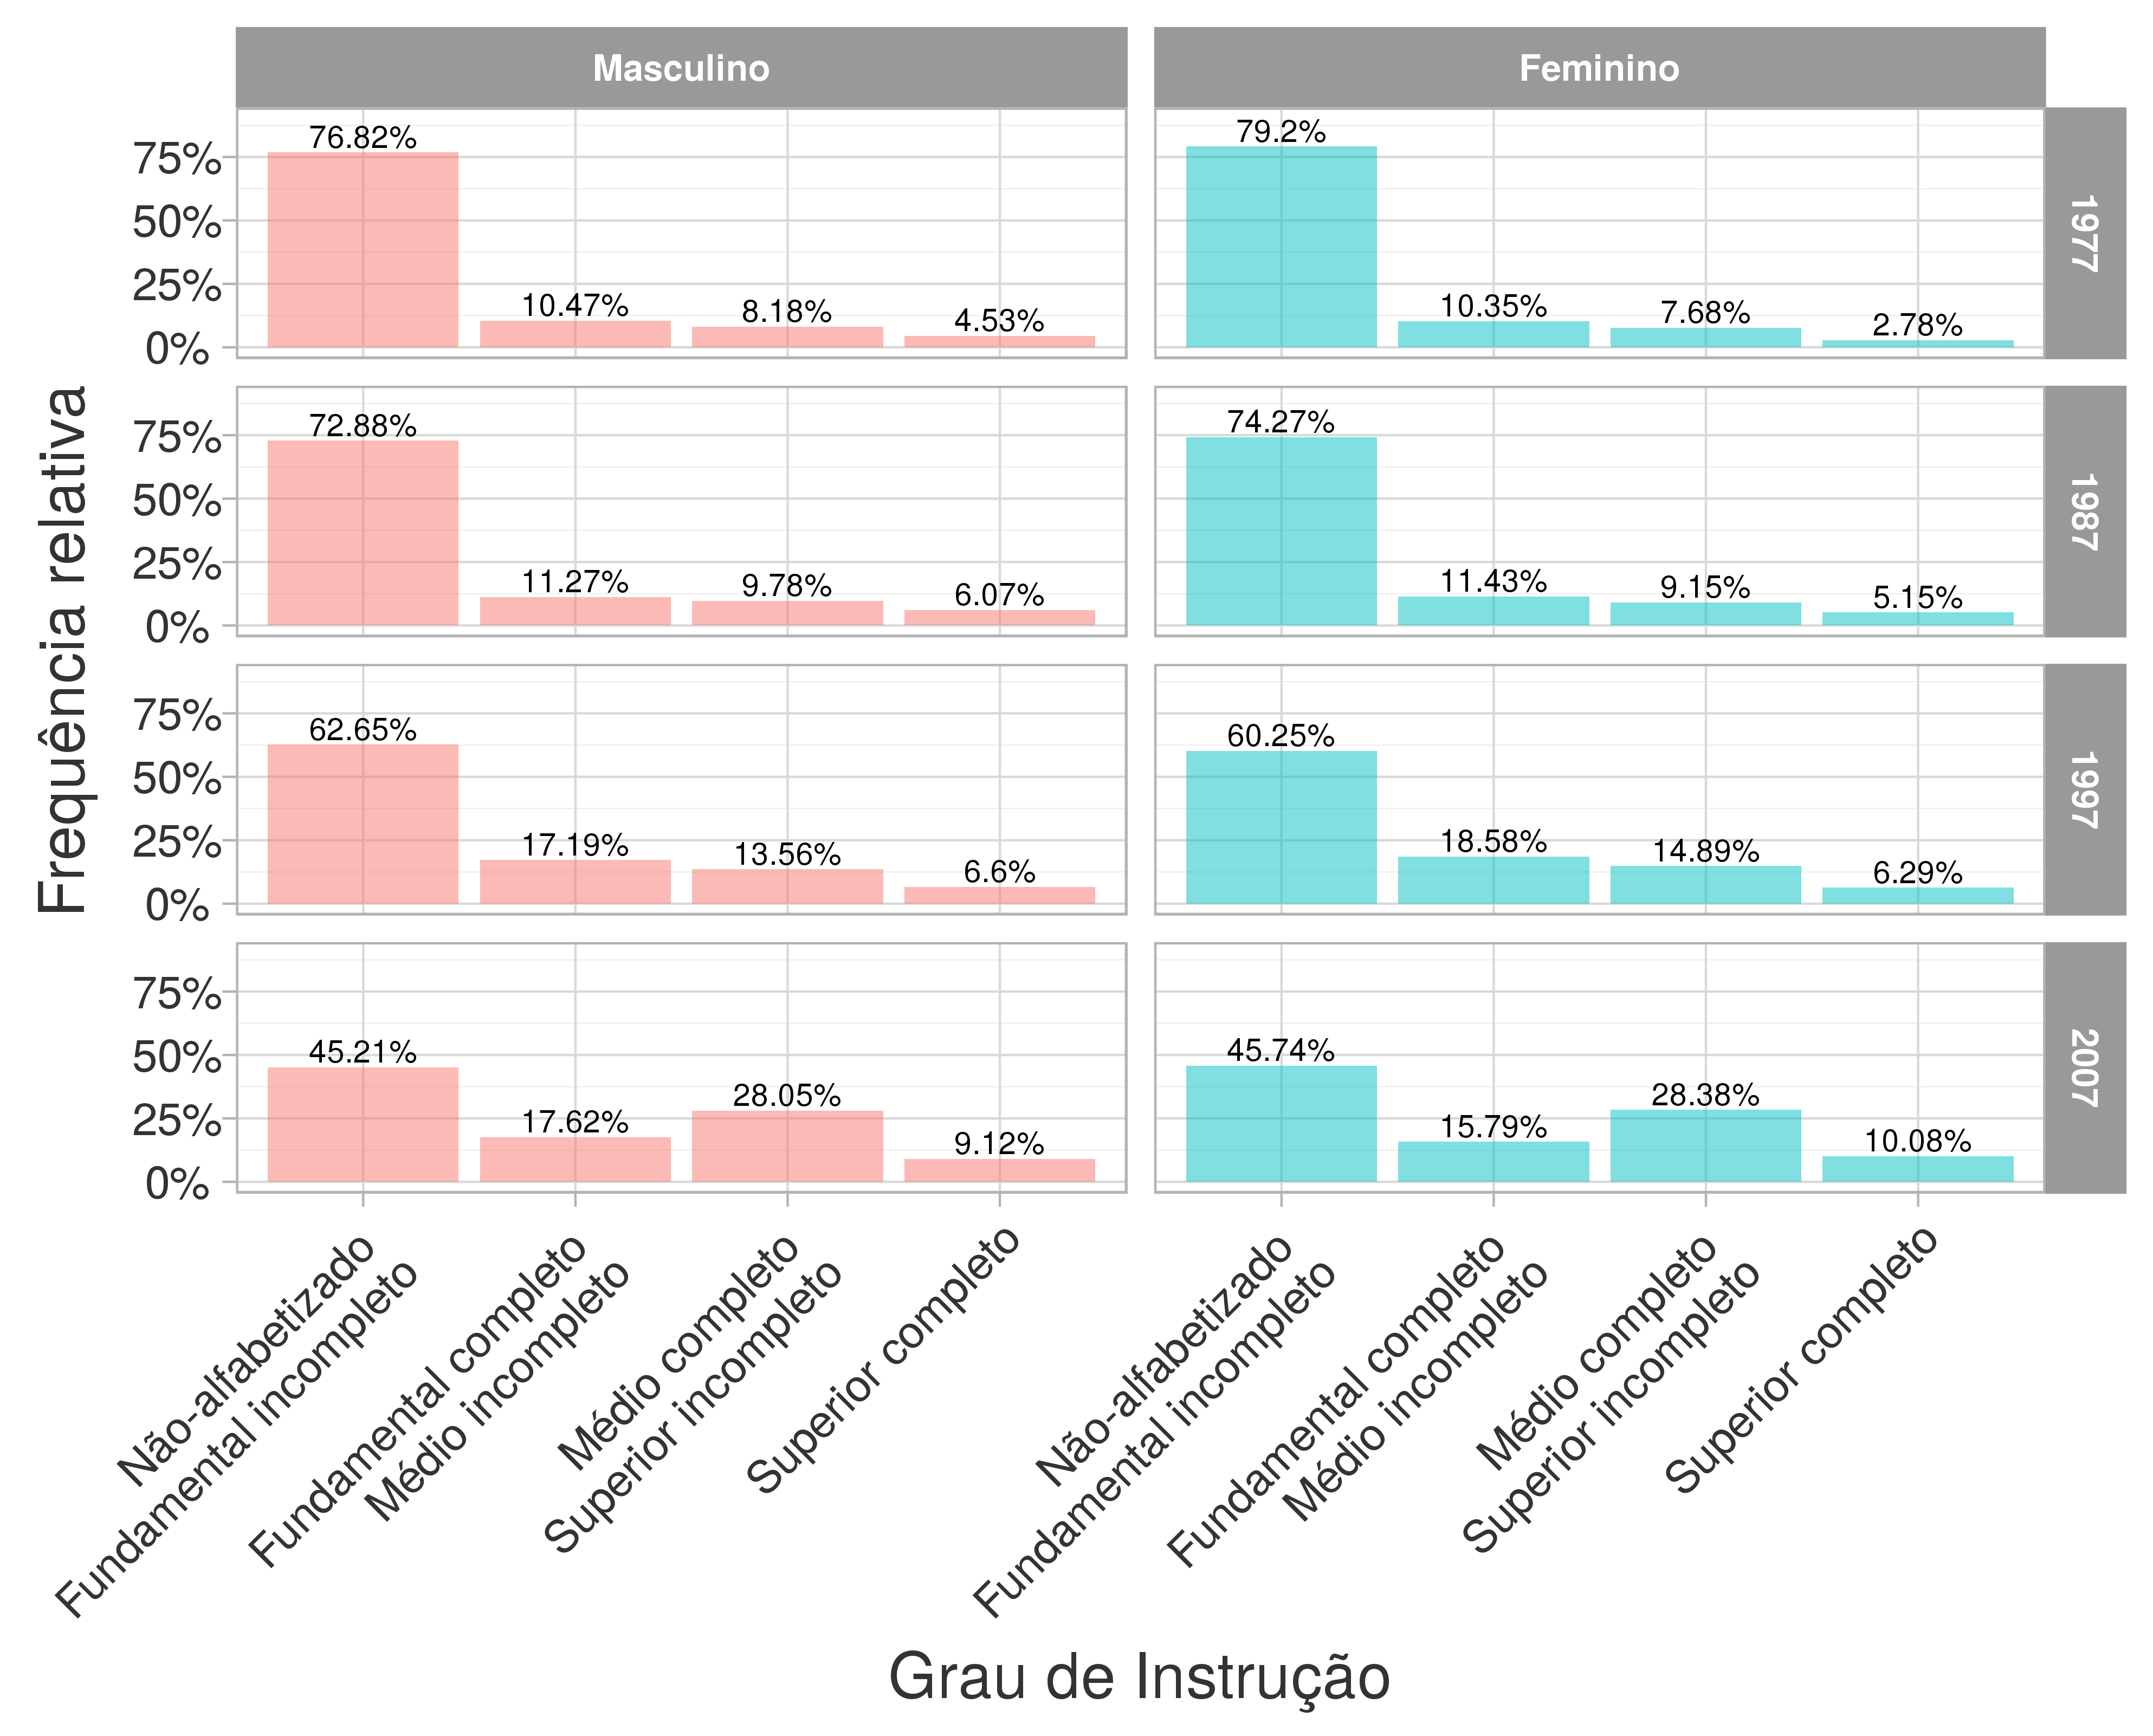
\includegraphics[width=0.97\textwidth]{./imagens/grau-instr.png}%
    \end{center}%
%    \fonte{Compilação própria}
\end{grafico}%

A elevação do grau de instrução entre 1977 e 2007 influencia não apenas as viagens motivo trabalho (por eventual aumento da empregabilidade) mas também as viagens motivo escola, realizadas por um contingente de pessoas cada vez maior, mais diverso e contendo mais faixas etárias.
A maior participação feminina no mercado de trabalho além de impactar as rendas (individual e familiar) deve influenciar bastante as viagens motivo trabalho. 

A renda individual (variável \textbf{REN_IND}) tem seu comportamento de médias e medianas análogo ao da renda familiar. Explora-se aqui, então, as rendas individuais de quem tem 10 anos ou mais%
\footnote{Foi adotada essa idade como limite de corte porque o IBGE produz estatísticas de ``valor do rendimento nominal médio mensal e mediano mensal para pessoas de 10 anos ou mais de idade, total e com rendimento''. Fonte: \url{http://www.sidra.ibge.gov.br/bda/tabela/listabl.asp?c=1381&z=cd&o=7} Acesso em 15 de janeiro de 2016}, 
segmentando por sexo e por duas situações familiares: pessoa responsável e cônjuge/companheiro(a).
Em os todos anos, a renda individual média masculina é superior à feminina para a mesma situação familiar, conforme Tabela \ref{tab:estat-ren-ind}. 
Em 1977, quando pessoa responsável pela família, o homem ganhava 2,5 vezes mais que a mulher em mesma condição. Essa marca vem caindo (cada vez mais devagar) até que, em 2007, eles ganham 1,5 vezes mais do que elas.
Para a situação de cônjuges, a relação entre as rendas médias masculina e feminina giram em média em torno de dois, oscilando para 1,8 em 1987 e 2,4 em 1997. Ou seja, homens cônjuges em geral ganham próximo do dobro das mulheres cônjuges, e essa situação pouco se alterou com o passar das décadas.

\begin{table}[htb]
\centering
   \IBGEtab{%\renewcommand{\arraystretch}{1.5}%%\ABNTEXfontereduzida%
        \renewcommand{\arraystretch}{1.5}
        \caption{Estatísticas da variável ``REN_IND''}
        \label{tab:estat-ren-ind}
    }{%

    \begin{tabular}{ccccccc}
        \toprule
        \textbf{Homem} & \multicolumn{3}{c}{\textbf{pessoa responsável}} & \multicolumn{3}{c}{\textbf{cônjuge/companheiro}} \\ \hline
        \textbf{ANO}   & \textbf{Média} & \textbf{Desvio Padrão} & \textbf{Mediana} & \textbf{Média} & \textbf{Desvio Padrão} & \textbf{Mediana} \\ \midrule \midrule
        \textbf{1977}  & 2.762,85 & 3.910,71 & 1.478,21 &   703,24 & 1.461,49 &   0,00 \\ \hline
        \textbf{1987}  & 1.610,76 & 2.146,33 &   985,80 &   522,67 &   953,85 &  99,64 \\ \hline
        \textbf{1997}  & 1.769,16 & 3.272,09 &   873,61 & 1.143,30 & 2.115,36 & 485,34 \\ \hline
        \textbf{2007}  & 1.265,37 & 2.330,39 &   600,00 & 1.147,71 & 2.396,79 & 300,00 \\ \hline                
        \textbf{Total} & 1.869,37 & 3.059,03 &   970,68 & 1.098,29 & 2.280,25 & 291,73 \\\bottomrule

        \textbf{Mulher} & \multicolumn{3}{c}{\textbf{pessoa responsável}} & \multicolumn{3}{c}{\textbf{cônjuge/companheira}} \\ \hline
        \textbf{ANO}   & \textbf{Média} & \textbf{Desvio Padrão} & \textbf{Mediana} & \textbf{Média} & \textbf{Desvio Padrão} & \textbf{Mediana} \\ \midrule \midrule
        \textbf{1977}  & 1.098,95 & 2.108,50 & 506,81 & 306,95 & 1.097,29 & 0,00 \\ \hline
        \textbf{1987}  &   807,79 & 1.398,68 & 397,99 & 284,87 &   872,94 & 0,00 \\ \hline
        \textbf{1997}  & 1.034,83 & 1.923,79 & 465,93 & 478,78 & 1.332,07 & 0,00 \\ \hline
        \textbf{2007}  &   866,43 & 1.661,52 & 380,00 & 498,39 & 1.204,76 & 0,00 \\ \hline                
        \textbf{Total} &   926,53 & 1.752,55 & 388,27 & 383,26 & 1.131,58 & 0,00 \\\bottomrule

    \end{tabular}
    
    }

\end{table}
% Estatísticas para registros com F_PESS==1, filtors em IDADE (>9), SEXO e SIT_FAM
% Não expandido com FE_PESS

\begin{grafico}[htb]%
    \caption{\label{graf:clas-econ-ren-ind}Distribuição da variável ``FAIXA_REN_IND'', por ano}%
        \begin{center}%
        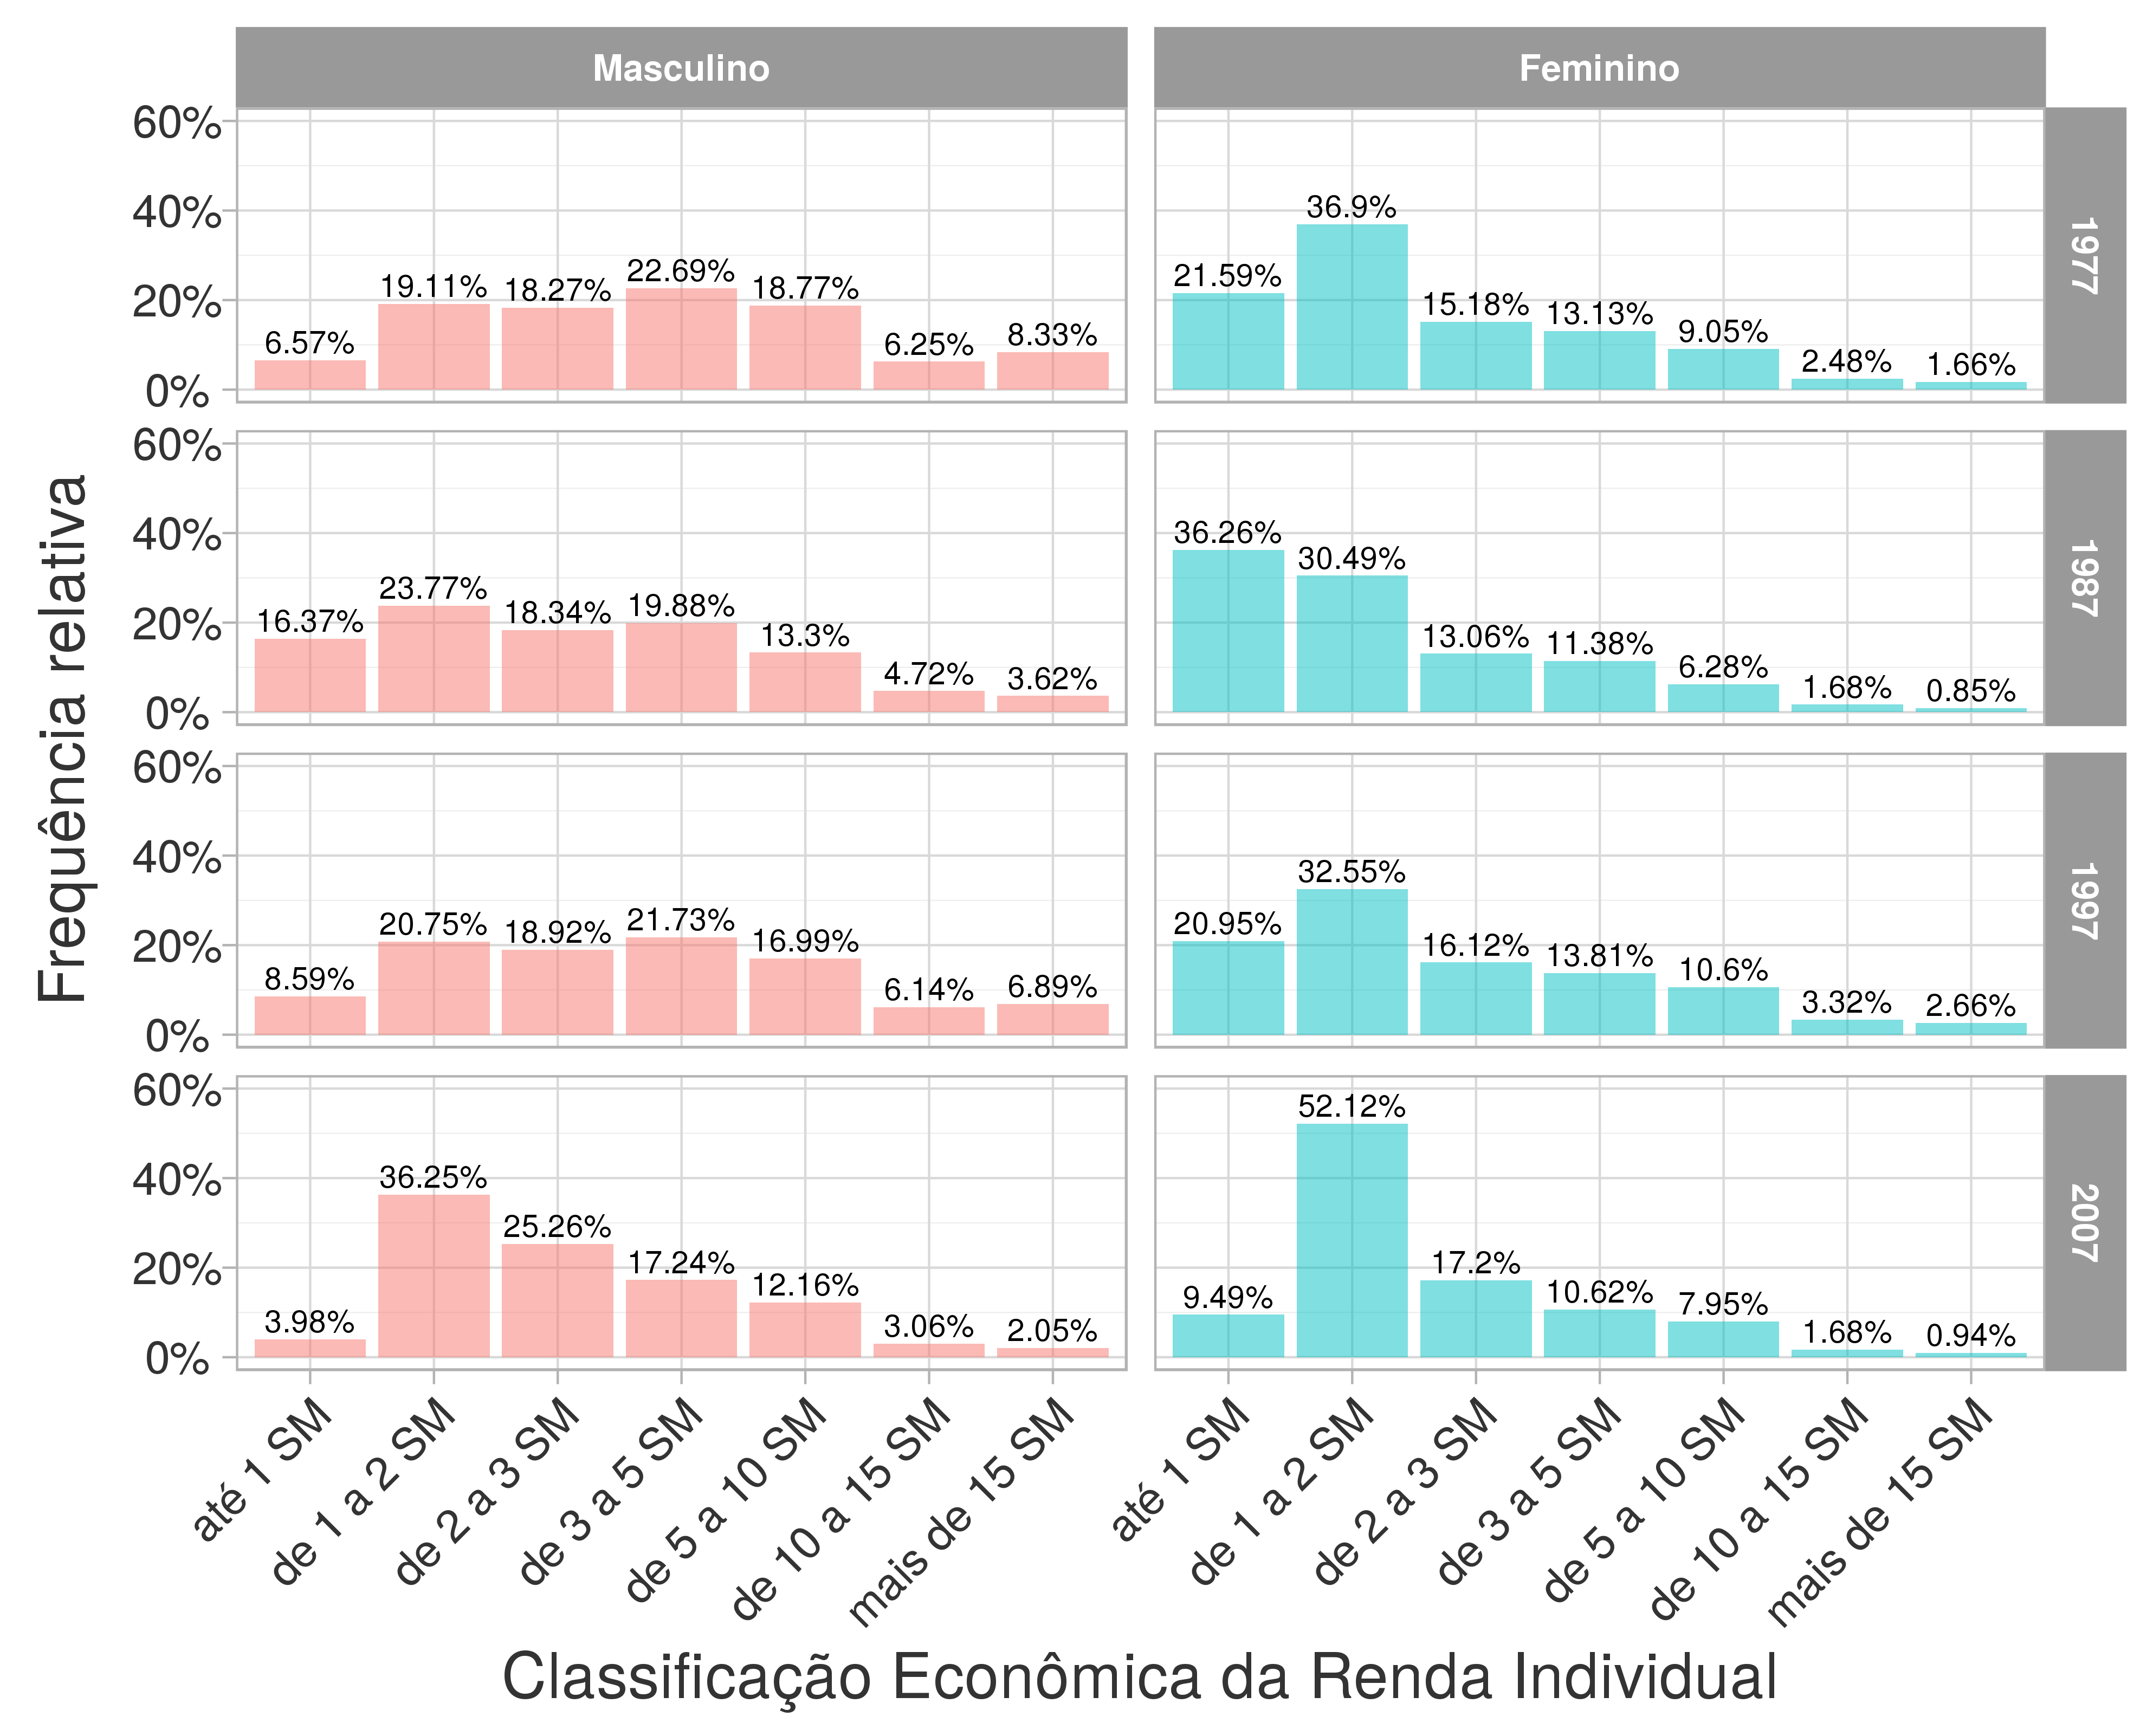
\includegraphics[width=1\textwidth]{./imagens/clas-econ-ren-ind.png}%
    \end{center}%
    %\fonte{Compilação própria}
\end{grafico}%

Pelo Gráfico \ref{graf:clas-econ-ren-ind} percebe-se que houve um aumento na quantidade de pessoas que ganhava até 1 salário mínimo entre 1977 e 1987. De 1987 para 2007 a proporção de pessoas que têm rendimentos nessa faixa salarial vem decrescendo. De 1977 a 1997 a faixa de rendimento de 1 a 2 salários mínimos ficou próxima dos 25\% e, em 2007, cresceu aproximadamente 10 pontos percentuais. Já a faixa de rendimento de 2 a 3 salários mínimos subiu cerca de 3 pontos percentuais entre 1977 e 2007, o mesmo que a faixa de rendimentos de 3 a 5 salários mínimos diminuiu no mesmo período.


\clearpage

\section{Análises Preliminares}\label{sec:analises-preliminares}

O grupo de análises que se segue busca compreender como é o comportamento das pessoas e das famílias em termo de viagens realizadas, em cada ano e diferencialmente entre os anos, olhando para tanto variáveis como:
\begin{compactitem}
\item número de viagens;
\item modos de viagem;
\item motivos de viagens;
\item duração das viagens;
\item distâncias das viagens.
\end{compactitem}

A variável \textbf{TOT_VIAG} representa o número total de viagens realizadas pela pessoa. Não existem \textit{missing values} neste campo, os valores mínimos para todos anos e ambos sexo são 0, bem como também são 0 os valores do primeiro quartil (25\%). Os valores das demais estatísticas (sem considerarr os fatores de expansão) estão apresentados na Tabela \ref{tab:estat-tot-viag}. Conforme já era de se esperar, para quem faz viagem no dia da pesquisa (número de viagem é não nulo) existe a predominância do valor 2, ou seja, são pessoas que saem de suas residências com um propósito único (trabalhar, estudar, fazer compras) e depois retornam à residência após a atividade.
Considerando toda a amostra, mesmo quem não fez viagem, percebe-se que, independente do sexo, o número médio de viagens por pessoa em relação a 1977 caiu um pouco em 1987 e 1997 (de 1,74 para 1,66) e subiu novamente em 2007 (para 1,86). Os desvios padrão caíram ao longo do tempo, indicando tendência de menor dispersão dos dados. Os valores de assimetria são positivos, indicando maior concentração à esquerda e cauda longa à direita da distribuição. Os valores de curtose evidenciam não tratar-se de distribuição normal.

Analisando esses dados segmentados por sexo, vê-se que as medianas são iguais. Os números médio e máximo de viagens para mulheres são sempre inferiores ao dos homens, para o mesmo ano. Os valores de assimetria para o sexo feminino e o masculino são positivos e convergem para o valor geral com o passar das décadas. 
A diferença entre o número médio de viagens de mulheres e homens vem diminuindo.

\begin{table}[htb]
   \IBGEtab{%\renewcommand{\arraystretch}{1.5}%%\ABNTEXfontereduzida%
        \renewcommand{\arraystretch}{1.5}
        \caption{Estatísticas da variável ``TOT_VIAG'', por ano e por sexo}
        \label{tab:estat-tot-viag}
    }{%

    \begin{tabular}{cccccccc}
        \toprule
        \textbf{Grupo} & \textbf{ANO}  & \textbf{Média} & \textbf{Desvio Padrão} & \textbf{Mediana} & \textbf{Máximo} & \textbf{Assimetria} & \textbf{Curtose} \\ \midrule \midrule
        \multirow{4}{*}{\textbf{\rotatebox[origin=c]{90}{Geral}}}
        & \textbf{1977}  & 1,74 & 1,82 & 2,00 & 24 & 1,52 & 4,91 \\ \cline{2-8}
        & \textbf{1987}  & 1,65 & 1,62 & 2,00 & 24 & 1,35 & 4,71 \\ \cline{2-8}
        & \textbf{1997}  & 1,66 & 1,63 & 2,00 & 21 & 1,36 & 4,34 \\ \cline{2-8}
        & \textbf{2007}  & 1,86 & 1,61 & 2,00 & 18 & 1,24 & 4,00 \\ \hline\hline
        \multirow{4}{*}{\textbf{\rotatebox[origin=c]{90}{Feminino}}}
        & \textbf{1977}  & 1,40 & 1,64 & 2,00 & 16 & 1,40 & 3,32 \\ \cline{2-8}
        & \textbf{1987}  & 1,43 & 1,59 & 2,00 & 19 & 1,38 & 3,92 \\ \cline{2-8}
        & \textbf{1997}  & 1,53 & 1,64 & 2,00 & 18 & 1,45 & 4,61 \\ \cline{2-8}
        & \textbf{2007}  & 1,75 & 1,64 & 2,00 & 17 & 1,23 & 3,48 \\ \hline\hline
        \multirow{4}{*}{\textbf{\rotatebox[origin=c]{90}{Masculino}}}
        & \textbf{1977}  & 2,10 & 1,92 & 2,00 & 24 & 1,56 & 5,55 \\ \cline{2-8}
        & \textbf{1987}  & 1,89 & 1,61 & 2,00 & 24 & 1,41 & 5,91 \\ \cline{2-8}
        & \textbf{1997}  & 1,79 & 1,60 & 2,00 & 21 & 1,29 & 4,22 \\ \cline{2-8}
        & \textbf{2007}  & 1,98 & 1,58 & 2,00 & 18 & 1,29 & 4,80 \\ \bottomrule            
    \end{tabular}%
    }{%
%		\fonte{Elaboração própria}
    \nota{Tabela elaborada considerando todas as pessoas da amostra, mesmo aquelas que não realizaram viagem, e sem realizar qualquer expansão}%
	}
	
\end{table}
% Estatísticas para registros com F_PESS==1, filtro por SEXO quando não tratar da informação geral
% Sem expansão

Ao considerar apenas quem relatou viagens no dia da pesquisa, os valores mínimos para todos anos e ambos sexo passam para 1, bem como também são 1 os valores do primeiro quartil (25\%). Os valores das demais estatísticas (considerando os fatores de expansão para a população) estão apresentados na Tabela \ref{tab:estat-tot-viag-nao-nula}.
Para todos os anos e para ambos sexos, as médias passaram para valores superiores a 2 e há uma pequena tendência de diminuição do número de viagens por pessoa com o passar do tempo.
Os desvios padrão caíram ao longo do tempo para as mulheres e para o conjunto de homens e mulheres, indicando menor dispersão dos dados. Os valores de assimetria aumentaram e continuaram positivos, indicando maior concentração à esquerda e cauda longa à direita da distribuição. Os valores de curtose também aumentaram e a distribuição continua não sendo aderente à normalidade.
Na segmentação por sexo, as medianas e a quantidade máxima de viagens permanecem iguais.
Entretanto, o número médio de viagens para mulheres era inferior ao dos homens em 1977 e 1987. Já em 1997 em 2007, a média delas passa a ser superior à deles.

\begin{table}[htb]
   \IBGEtab{%\renewcommand{\arraystretch}{1.5}%%\ABNTEXfontereduzida%
        \renewcommand{\arraystretch}{1.5}
        \caption{Estatísticas da variável ``TOT_VIAG'', por ano e por sexo, considerando apenas quem fez viagem}
        \label{tab:estat-tot-viag-nao-nula}
    }{%

    \begin{tabular}{cccccccc}
        \toprule
        \textbf{Grupo} & \textbf{ANO}  & \textbf{Média} & \textbf{Desvio Padrão} & \textbf{Mediana} & \textbf{Máximo} & \textbf{Assimetria} & \textbf{Curtose} \\ \midrule \midrule
        \multirow{4}{*}{\textbf{\rotatebox[origin=c]{90}{Geral}}}
        & \textbf{1977}  & 2,82 & 1,52 & 2,00 & 24 & 2,65 & 11,39 \\ \cline{2-8}
        & \textbf{1987}  & 2,62 & 1,27 & 2,00 & 24 & 3,95 & 14,38 \\ \cline{2-8}
        & \textbf{1997}  & 2,61 & 1,30 & 2,00 & 21 & 2,83 & 12,28 \\ \cline{2-8}
        & \textbf{2007}  & 2,64 & 1,28 & 2,00 & 18 & 2,73 & 11,08 \\ \hline \hline
        \multirow{4}{*}{\textbf{\rotatebox[origin=c]{90}{Feminino}}}
        & \textbf{1977}  & 2,67 & 1,31 & 2,00 & 16 & 2,48 & 11,19 \\ \cline{2-8}
        & \textbf{1987}  & 2,61 & 1,25 & 2,00 & 19 & 2,81 & 15,66 \\ \cline{2-8}
        & \textbf{1997}  & 2,63 & 1,31 & 2,00 & 18 & 2,92 & 12,39 \\ \cline{2-8}
        & \textbf{2007}  & 2,65 & 1,29 & 2,00 & 17 & 2,64 & 12,18 \\ \hline \hline
        \multirow{4}{*}{\textbf{\rotatebox[origin=c]{90}{Masculino}}}
        & \textbf{1977}  & 2,93 & 1,65 & 2,00 & 24 & 2,61 & 11,09 \\ \cline{2-8}
        & \textbf{1987}  & 2,62 & 1,30 & 2,00 & 24 & 3,05 & 15,66 \\ \cline{2-8}
        & \textbf{1997}  & 2,59 & 1,29 & 2,00 & 21 & 2,75 & 11,39 \\ \cline{2-8}
        & \textbf{2007}  & 2,62 & 1,28 & 2,00 & 18 & 2,82 & 12,18 \\\bottomrule             
    \end{tabular}
    }{%
%		\fonte{Elaboração própria}
    \nota{Tabela elaborada considerando apenas as pessoas da amostra que realizaram viagem, e sem realizar qualquer expansão}%
	}%
	
\end{table}
% Estatísticas para registros com F_PESS==1, filtro por SEXO quando não tratar da informação geral
% Sem expansão

\begin{table}[htb]
   \IBGEtab{%\renewcommand{\arraystretch}{1.5}%%\ABNTEXfontereduzida%
        \renewcommand{\arraystretch}{1.5}
        \caption{Média da variável ``TOT_VIAG'', por ano e por sexo, com expansão}
        \label{tab:estat-tot-viag-modelo-od}
    }{%

    \begin{tabular}{P{2.0cm}P{2.0cm}P{4.0cm}P{4.0cm}}
        \toprule
          \textbf{Grupo} &
          \textbf{ANO} &
          \quebraLinhaCel{\textbf{Pessoas com ou}\\\textbf{sem viagem}} &
          \quebraLinhaCel{\textbf{Apenas Pessoas}\\\textbf{com viagem}}\\
        \midrule \midrule
          \multirow{4}{*}{\textbf{\rotatebox[origin=c]{90}{Geral}}}
          & \textbf{1977}  & 2,07 & 3,42 \\ \cline{2-4}
          & \textbf{1987}  & 2,06 & 3,28 \\ \cline{2-4}
          & \textbf{1997}  & 1,87 & 2,94 \\ \cline{2-4}
          & \textbf{2007}  & 1,95 & 2,86 \\ \hline \hline
        \multirow{4}{*}{\textbf{\rotatebox[origin=c]{90}{Feminino}}}
          & \textbf{1977}  & 1,67 & 3,24 \\ \cline{2-4}
          & \textbf{1987}  & 1,79 & 3,27 \\ \cline{2-4}
          & \textbf{1997}  & 1,73 & 2,96 \\ \cline{2-4}
          & \textbf{2007}  & 1,85 & 2,89 \\ \hline \hline
        \multirow{4}{*}{\textbf{\rotatebox[origin=c]{90}{Masculino}}}
          & \textbf{1977}  & 2,50 & 3,55 \\ \cline{2-4}
          & \textbf{1987}  & 2,36 & 3,28 \\ \cline{2-4}
          & \textbf{1997}  & 2,03 & 2,92 \\ \cline{2-4}
          & \textbf{2007}  & 2,07 & 2,82 \\
        \bottomrule
       
    \end{tabular}
    }{%
%		\fonte{Elaboração própria}
    \nota{Dados obtidos pela expansão utilizada nos relatórios oficiais das Pesquisas OD, que consiste em calcular a média com base na equação$\frac{\sum{(FE\_VIAG)}}{\sum{(FE\_PESS*F\_PESS)}}$}%
	}%
	
\end{table}
% Estatísticas seguindo exemplo metrô
% Com expansão por FE_VIAG e FE_PESS

Foram feitos testes t para avaliar se as médias de mulheres e de homens eram estatisticamente diferentes, em cada ano, tanto considerando quem não fez viagem \mbox{(TOT_VIAG=0)}, como desconsiderando esse caso. Os p-valores resultantes foram todos inferiores a 0,05, logo, rejeitou-se a hipótese nula de que as médias seriam iguais (nível de confiança de 95\%).
Foram feitos testes t para avaliar se as médias entre os anos eram diferentes, para o grupo de mulheres, tanto considerando quem não fez viagem \mbox{(TOT_VIAG=0)}, como desconsiderando esse caso. Também aqui os p-valores resultantes foram todos inferiores a 0,05, logo, rejeitou-se a hipótese nula de que as médias seriam iguais (nível de confiança de 95\%). 
Portanto, ao considerar o efeito de quem não sai de casa, o número médio de viagens das mulheres sempre é menor que o dos homens, para um dado ano, e realmente houve aumento no número médio de viagens das mulheres, da ordem de 0,1 viagem/década.
Ao desconsiderar o efeito de quem não sai de casa, o número médio de viagens das mulheres tornou-se maior que o dos homens em 1997 e o número médio de viagens de homens e mulheres cai com o tempo.

O Gráfico \ref{graf:distr-num-viag} apresenta a distribuição de viagens (considerando os fatores de expansão para a população) até o limite de 6 viagens, corte feito apenas para melhorar a visualização do gráfico, já que a cauda é bastante longa. 
Deste gráfico, vale destacar a relação entre as viagens nulas (quem não sai de casa) e as viagens de ida e volta (valores iguais a 2). Para homens, o número de viagens nulo é menos frequente que o número de viagens de valor 2 para todos anos de análise. Já para as mulheres, em 1977 as viagens nulas eram a maioria, indicando certa fixitude delas na residência. Essa porcentagem vai diminuindo e a porcentagem no número de viagens igual a 2 vai crescendo, ficam próximas em 1997 e, em 2007, inverte-se a situação observada em 1977.
Provavelmente devido à maior participação no mercado de trabalho, as mulheres ganharam mobilidade, restringindo-se menos ao espaço doméstico.

\begin{grafico}[htb]%
    \caption{\label{graf:distr-num-viag}Distribuição da variável ``TOT_VIAG'' por ano e por sexo}%
    \begin{center}%
        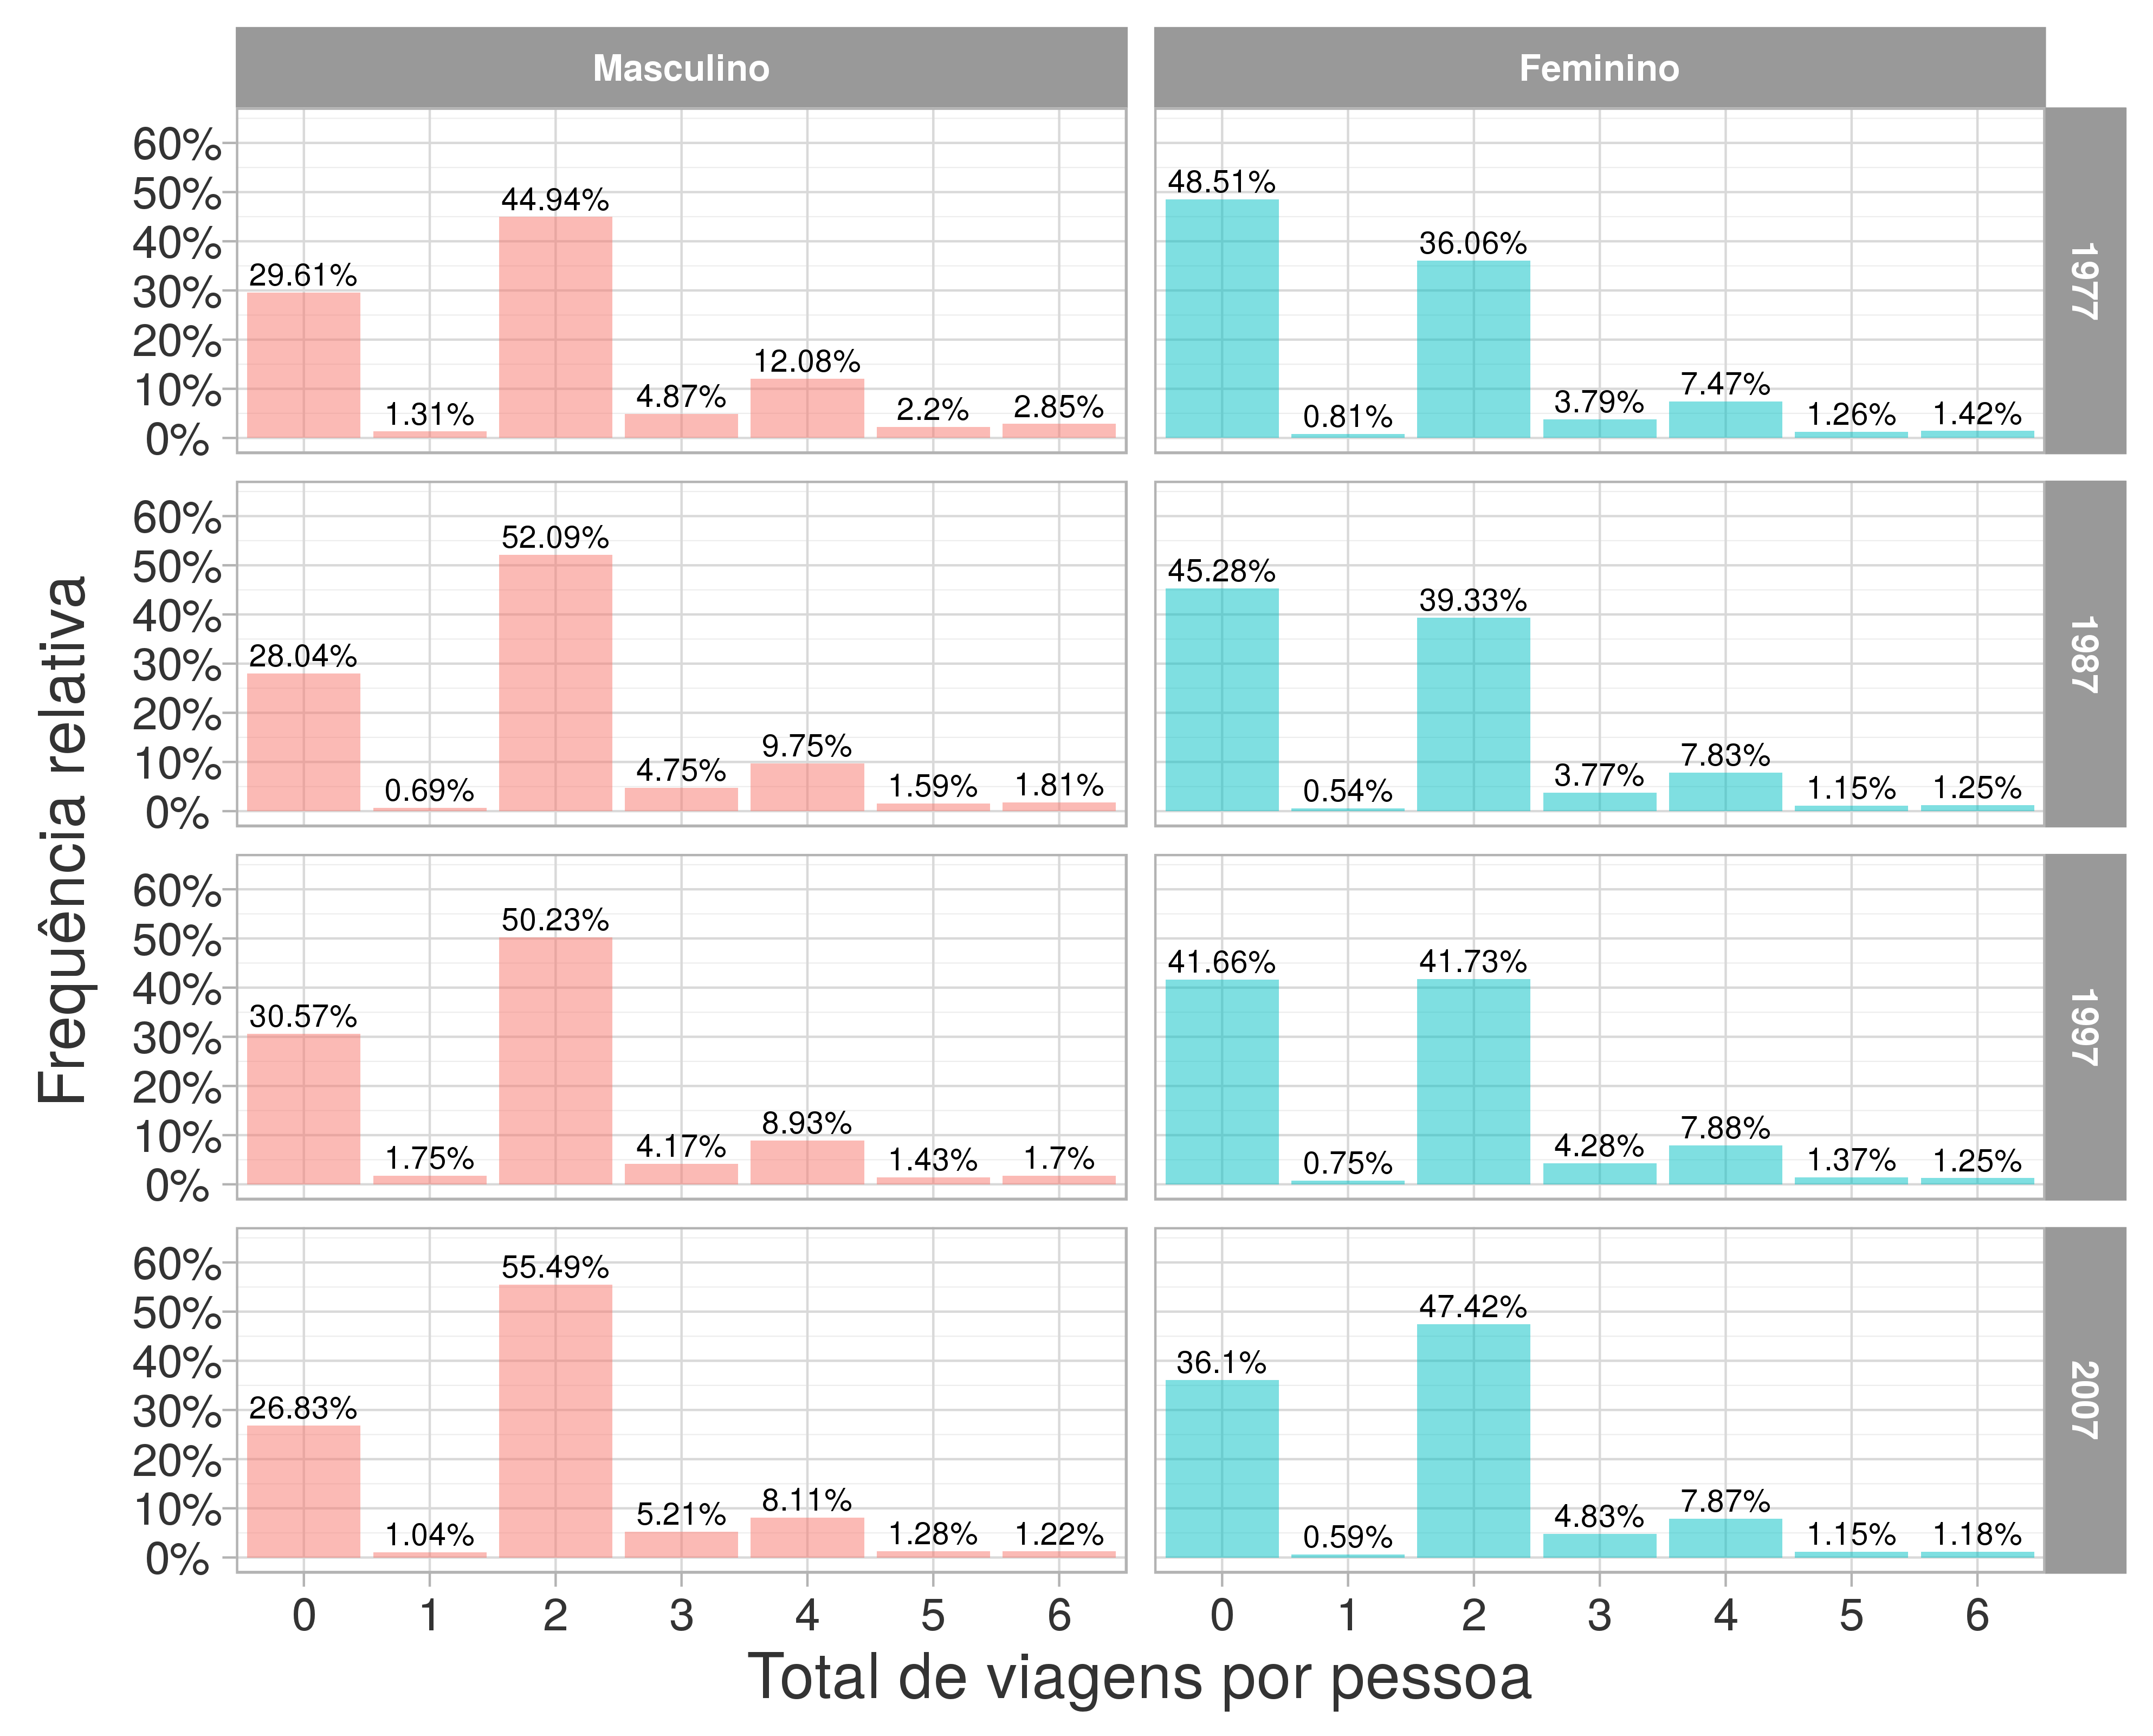
\includegraphics[width=1\textwidth]{./imagens/tot-viag-pess.png}%
    \end{center}%
%    \fonte{Compilação própria}
\end{grafico}%
% Estatísticas para registros com F_PESS==1 e SEXO
% Expandido com FE_PESS

\newpage
Ao focar no agregado da família, os valores das principais estatísticas (considerando os fatores de expansão para a população) da variável \textbf{FAM_VIAG_TOT} estão apresentados na Tabela \ref{tab:estat-fam-viag-tot}.
O número médio de viagens da família com ao longo do tempo, comportamento consistente tanto com a queda do número médio de viagens por pessoa (Tabelas \ref{tab:estat-tot-viag} e \ref{tab:estat-tot-viag-nao-nula}) quanto com a diminuição do tamanho da família (Tabela \ref{tab:estat-tot-pess}).
Aqui também os desvios padrão caem ao longo do tempo (tendência de menor dispersão de dados) e os valores de assimetria são positivos (maior concentração à esquerda e cauda longa à direita da distribuição). Os valores de curtose indicam que a distribuição não é normal.
Ao retirar aquelas famílias com total de viagens nulo (ninguém fez viagem), não se observam diferenças nas tendências das estatísticas, à exceção da mediana que em 1997 era 7 em 1997 e passa para 6 ao inserir famílias cujo total de viagens é zero.

\begin{table}[htb]
\centering
   \IBGEtab{%\renewcommand{\arraystretch}{1.5}%%\ABNTEXfontereduzida%
        \renewcommand{\arraystretch}{1.5}
        \caption{Estatísticas da variável ``FAM_VIAG_TOT'', por ano}
        \label{tab:estat-fam-viag-tot}
    }{%

    \begin{tabular}{ccccccc}
        \toprule
        \multicolumn{7}{c}{\textbf{Considerando famílias em que há pela menos uma viagem}} \\ \hline
        \textbf{ANO} & \textbf{Média} & \textbf{Desvio Padrão} & \textbf{Mediana} & \textbf{Máximo} & \textbf{Assimetria} & \textbf{Curtose} \\ \midrule \midrule
        \textbf{1977} & 8,97 & 6,00 & 8,00 & 59 & 1,36 & 2,90 \\ \hline
        \textbf{1987} & 8,04 & 5,14 & 7,00 & 50 & 1,39 & 3,43 \\ \hline
        \textbf{1997} & 7,68 & 4,80 & 7,00 & 45 & 1,29 & 2,85 \\ \hline
        \textbf{2007} & 7,11 & 4,31 & 6,00 & 68 & 1,52 & 6,84 \\\bottomrule          

        \multicolumn{7}{c}{\textbf{Considerando inclusive família em que ninguém fez viagem}} \\ \hline
        \textbf{ANO}  & \textbf{Média} & \textbf{Desvio Padrão} & \textbf{Mediana} & \textbf{Máximo} & \textbf{Assimetria} & \textbf{Curtose} \\ \midrule \midrule
        \textbf{1977} & 8,58 & 6,14 & 8,00 & 59 & 1,27 & 2,62 \\ \hline
        \textbf{1987} & 7,71 & 5,28 & 7,00 & 50 & 1,27 & 3,05 \\ \hline
        \textbf{1997} & 7,22 & 5,00 & 6,00 & 45 & 1,14 & 2,39 \\ \hline
        \textbf{2007} & 6,62 & 4,53 & 6,00 & 68 & 1,28 & 5,38 \\\bottomrule

    \end{tabular}
    }{%
%		\fonte{Elaboração própria}
	}
\end{table}
% Estatísticas para registros com F_FAM==1, filtro por ANO
% Expandido com FE_FAM

\newpage
Nos campos MODO1, MODO2, MODO3 e MODO4 a categoria ``ônibus de linha'' inclui as categorias originais ``ônibus trólebus'', ``trólebus'', ``ônibus diesel'', ``ônibus'', ``ônibus município de São Paulo'', ``ônibus outros municípios'' e ``ônibus metropolitano''. A categoria ``ônibus escolar/empresa'' inclui também as categorias originais ``ônibus fretado'', ``escolar'', ``transporte escolar``. A categoria ``lotação/van'' inclui as categorias originais ``lotação/perua'', ``microônibus/van município de São Paulo'', ``microônibus/van outros municípios'' e ``microônibus/van metropolitano''. Vale lembrar que para os anos de 1977 e 1987 foram levantados no máximo três modos, e para os anos 1997 e 2007, no máximo quatro modos para cada viagem.

Na Tabela \ref{tab:estat-modos} foram agrupados em ``alta capacidade'' os modos metroferroviários (metrô e trem), em ``ônibus'' todos os tipos de ônibus (de linha, escolar, de empresas, lotações e vans), em ``passageiro de automóvel'' os passageiros de automóvel particular e também de táxis, em ``Outros'' as viagens realizadas por motocicletas e bicicletas pois estas foram diagnosticadas apenas para 2007. Nesta tabela estão apresentadas as frequências relativas destes agrupamentos para o \textbf{MODO1} (primeiro modo utilizado na viagem) e também para o \textbf{MODO2} (segundo modo utilizado), buscando avaliar a divisão modal por ano, para quem realizou viagem. Assim, para o primeiro modo o total soma 100\% em todos anos, mas o total por ano do segundo modo em diante não necessariamente, porque nem todas viagens utilizaram mais de um modo.


\begin{table}[htb]
\centering
   \IBGEtab{%\renewcommand{\arraystretch}{1.5}%%\ABNTEXfontereduzida%
        \renewcommand{\arraystretch}{1.5}
        \caption{Frequência relativa das variáveis ``MODO1'' e ``MODO2'', por ano}
        \label{tab:estat-modos}
    }{%

    \begin{tabular}{cccccccc}
        \toprule
        \textbf{MODO 1} & \textbf{Alta}       & \textbf{}       & \textbf{Dirigindo} &  \textbf{Passageiro}  & \textbf{}     & \textbf{}  & \textbf{} \\
        \textbf{ANO}    & \textbf{Capacidade} & \textbf{Ônibus} & \textbf{Automóvel} & \textbf{de Automóvel} & \textbf{A pé} & \textbf{Outros} & \textbf{Total} \\ \midrule \midrule
        \textbf{1977}  & 3,0\% & 41,7\% & 15,4\% & 11,3\% & 28,0\% & 0,8\% & 100\% \\ \hline
        \textbf{1987}  & 4,7\% & 30,5\% & 17,2\% &  9,7\% & 36,2\% & 1,7\% & 100\% \\ \hline
        \textbf{1997}  & 6,4\% & 28,9\% & 20,5\% & 10,8\% & 34,4\% & 1,3\% & 100\% \\ \hline
        \textbf{2007}  & 7,0\% & 31,8\% & 19,2\% &  8,6\% & 33,1\% & 2,9\% & 100\% \\\bottomrule          

        \textbf{MODO 2}      & \textbf{Alta}       & \textbf{}       & \textbf{Dirigindo} &  \textbf{Passageiro}  & \textbf{}     & \textbf{}  & \textbf{} \\
        \textbf{ANO}   & \textbf{Capacidade} & \textbf{Ônibus} & \textbf{Automóvel} & \textbf{de Automóvel} & \textbf{A pé} & \textbf{Outros} & \textbf{Total} \\ \midrule \midrule
        \textbf{1977}  & 2,0\% & 7,0\% & 0,1\% & 0,2\% & - & 0,0\% &  9,2\% \\ \hline
        \textbf{1987}  & 3,6\% & 6,5\% & 0,1\% & 0,1\% & - & 0,0\% & 10,3\% \\ \hline
        \textbf{1997}  & 3,5\% & 5,9\% & 0,0\% & 0,1\% & - & 0,0\% &  9,5\% \\ \hline
        \textbf{2007}  & 4,2\% & 8,2\% & 0,1\% & 0,1\% & - & 0,0\% & 12,5\% \\\bottomrule    
      
    \end{tabular}
    }{%
%		\fonte{Elaboração própria}
	}
\end{table}
% Estatísticas para registros com F_VIAG==1
% Expandido com FE_VIAG

Em relação à utilização do automóvel, sua proporção sobe cerca de 5\% de 1977 até 1997 e cai pouco mais de 1\% em 2007, talvez por conta dos congestionamentos cada vez mais frequentes e da evolução do sistema de transporte coletivo público da RMSP. Quando utilizado, o carro é quase sempre o único modo da viagem.
Os ônibus têm uma queda de $\sim$ 13\% pontos percentuais entre 1977 e 1997, com recuperação de $\sim$ 3\% em 2007. Quem deixou de utilizar o ônibus nas primeiras 3 décadas passou a utilizar a caminhada como método de deslocamento ($\sim$ 6\%), ou o carro ($\sim$ 5\%) o ainda o transporte coletivo de alta capacidade ($\sim$ 3\%).
Os modos metrô e trem vêm recebendo um incremento de viagens década a década, saindo de 3\% em 1977 para 7\% em 2077. A contribuição baixa deste modo, apesar de sua alta capacidade, deve-se provavelmente à cobertura insuficiente e pouca capilaridade no tecido urbano.
Vale ressaltar que ``alta capacidade'' é o único modo que tem sua utilização ainda muito presente como segundo modo (relação MODO1/MODO2 $\sim$ 1,5) - as viagens de ônibus são reduzidas pelo menos da ordem de um quarto, as de carro e outros caem a quase 0\% no segundo modo.
Isto significa que as viagens com metrô e trem são mais frequentemente precedidas de viagens com outro modo (principalmente ônibus), funcionando como tronco numa lógica de sistema tronco-alimentador.
As viagens a pé aumentaram percentualmente entre 1977 e 1997 e caíram em 2007, talvez pelas distâncias necessárias de viagem dado o crescimento da área metropolitana de São Paulo. Conforme o conceito de viagem a pé anteriormente exposto, não haverá modo a pé nos modos 2, 3 ou 4.
As tabelas de contingência dos modos 3 e 4 não serão apresentadas por serem pouco significativos no contexto geral: o modo 3 varia de 0,9\% (em 1977) a 2,8\% (2007) do total de viagens, sendo predominante o modo ônibus; o modo 4, só existente em 1997 e 2007, aparece em 0,4\% das viagens realizadas.

Os Gráficos \ref{graf:freq-modo1} e \ref{graf:freq-modo2} apresentam a segmentação por sexo dos modos 1 e 2 de viagem, respectivamente.
No primeiro modo de viagem, as viagens a pé são o modo mais frequente para as mulheres em 1987, 1997 e 2007, somente em 1977 o ônibus era mais frequentemente utilizado por elas.
Para os homens, o modo mais frequente em 1977 e 2007 é o ônibus, e em 1987 e 1997, a pé.
O modo outros é o menos frequente em 1977, 1987 e 1997 para ambos os sexos; em 2007, eles superam a alta capacidade, provavelmente porque o transporte por motocicleta e bicicleta passou a ser mais expressivo.
Comparando ambos os sexos por categoria do primeiro modo:
\begin{compactitem}[]
\item (i) As mulheres sempre fizeram mais viagens a pé que os homens: a diferença de 6,7 pontos percentuais de 1977 aumenta para 11,3 em 1987, cai para 7,9 em 1997 e sobe novamente em 2007 para 8,8\%.
\item (ii) A utilização feminina do ônibus é quase sempre superior á masculina, exceto em 1987, ano em que as proporções praticamente se igualam e desde quando a diferença vem aumentando com o tempo.
\item (iii) É na utilização do automóvel em que residem as diferenças mais gritantes entre os gêneros: homens predominantemente motoristas e mulheres, passageiras. O destaque aqui reside no fato que entre 1997 e 2007, dentro do grupo de mulheres, elas passaram a dirigir mais do que ser passageiras de automóvel.
\item (iv) A participação do transporte de alta capacidade gira em torno de 2,5\% a 5,5\% do \textit{share} modal, com o homem tendo uma utilização um pouco mais frequente dentro do seu grupo do que as mulheres, mais devido ao trem (cujos percentuais dos homens são sempre superiores aos das mulheres) do que ao Metrô (onde os percentuais das mulheres supera o dos homens a partir de 1997).
\end{compactitem}

\begin{grafico}[htb]%
    \caption{\label{graf:freq-modo1}Proporção das viagens do sexo feminino e do sexo masculino, segundo o primeiro modo da viagem, por ano}%
    \begin{center}%
        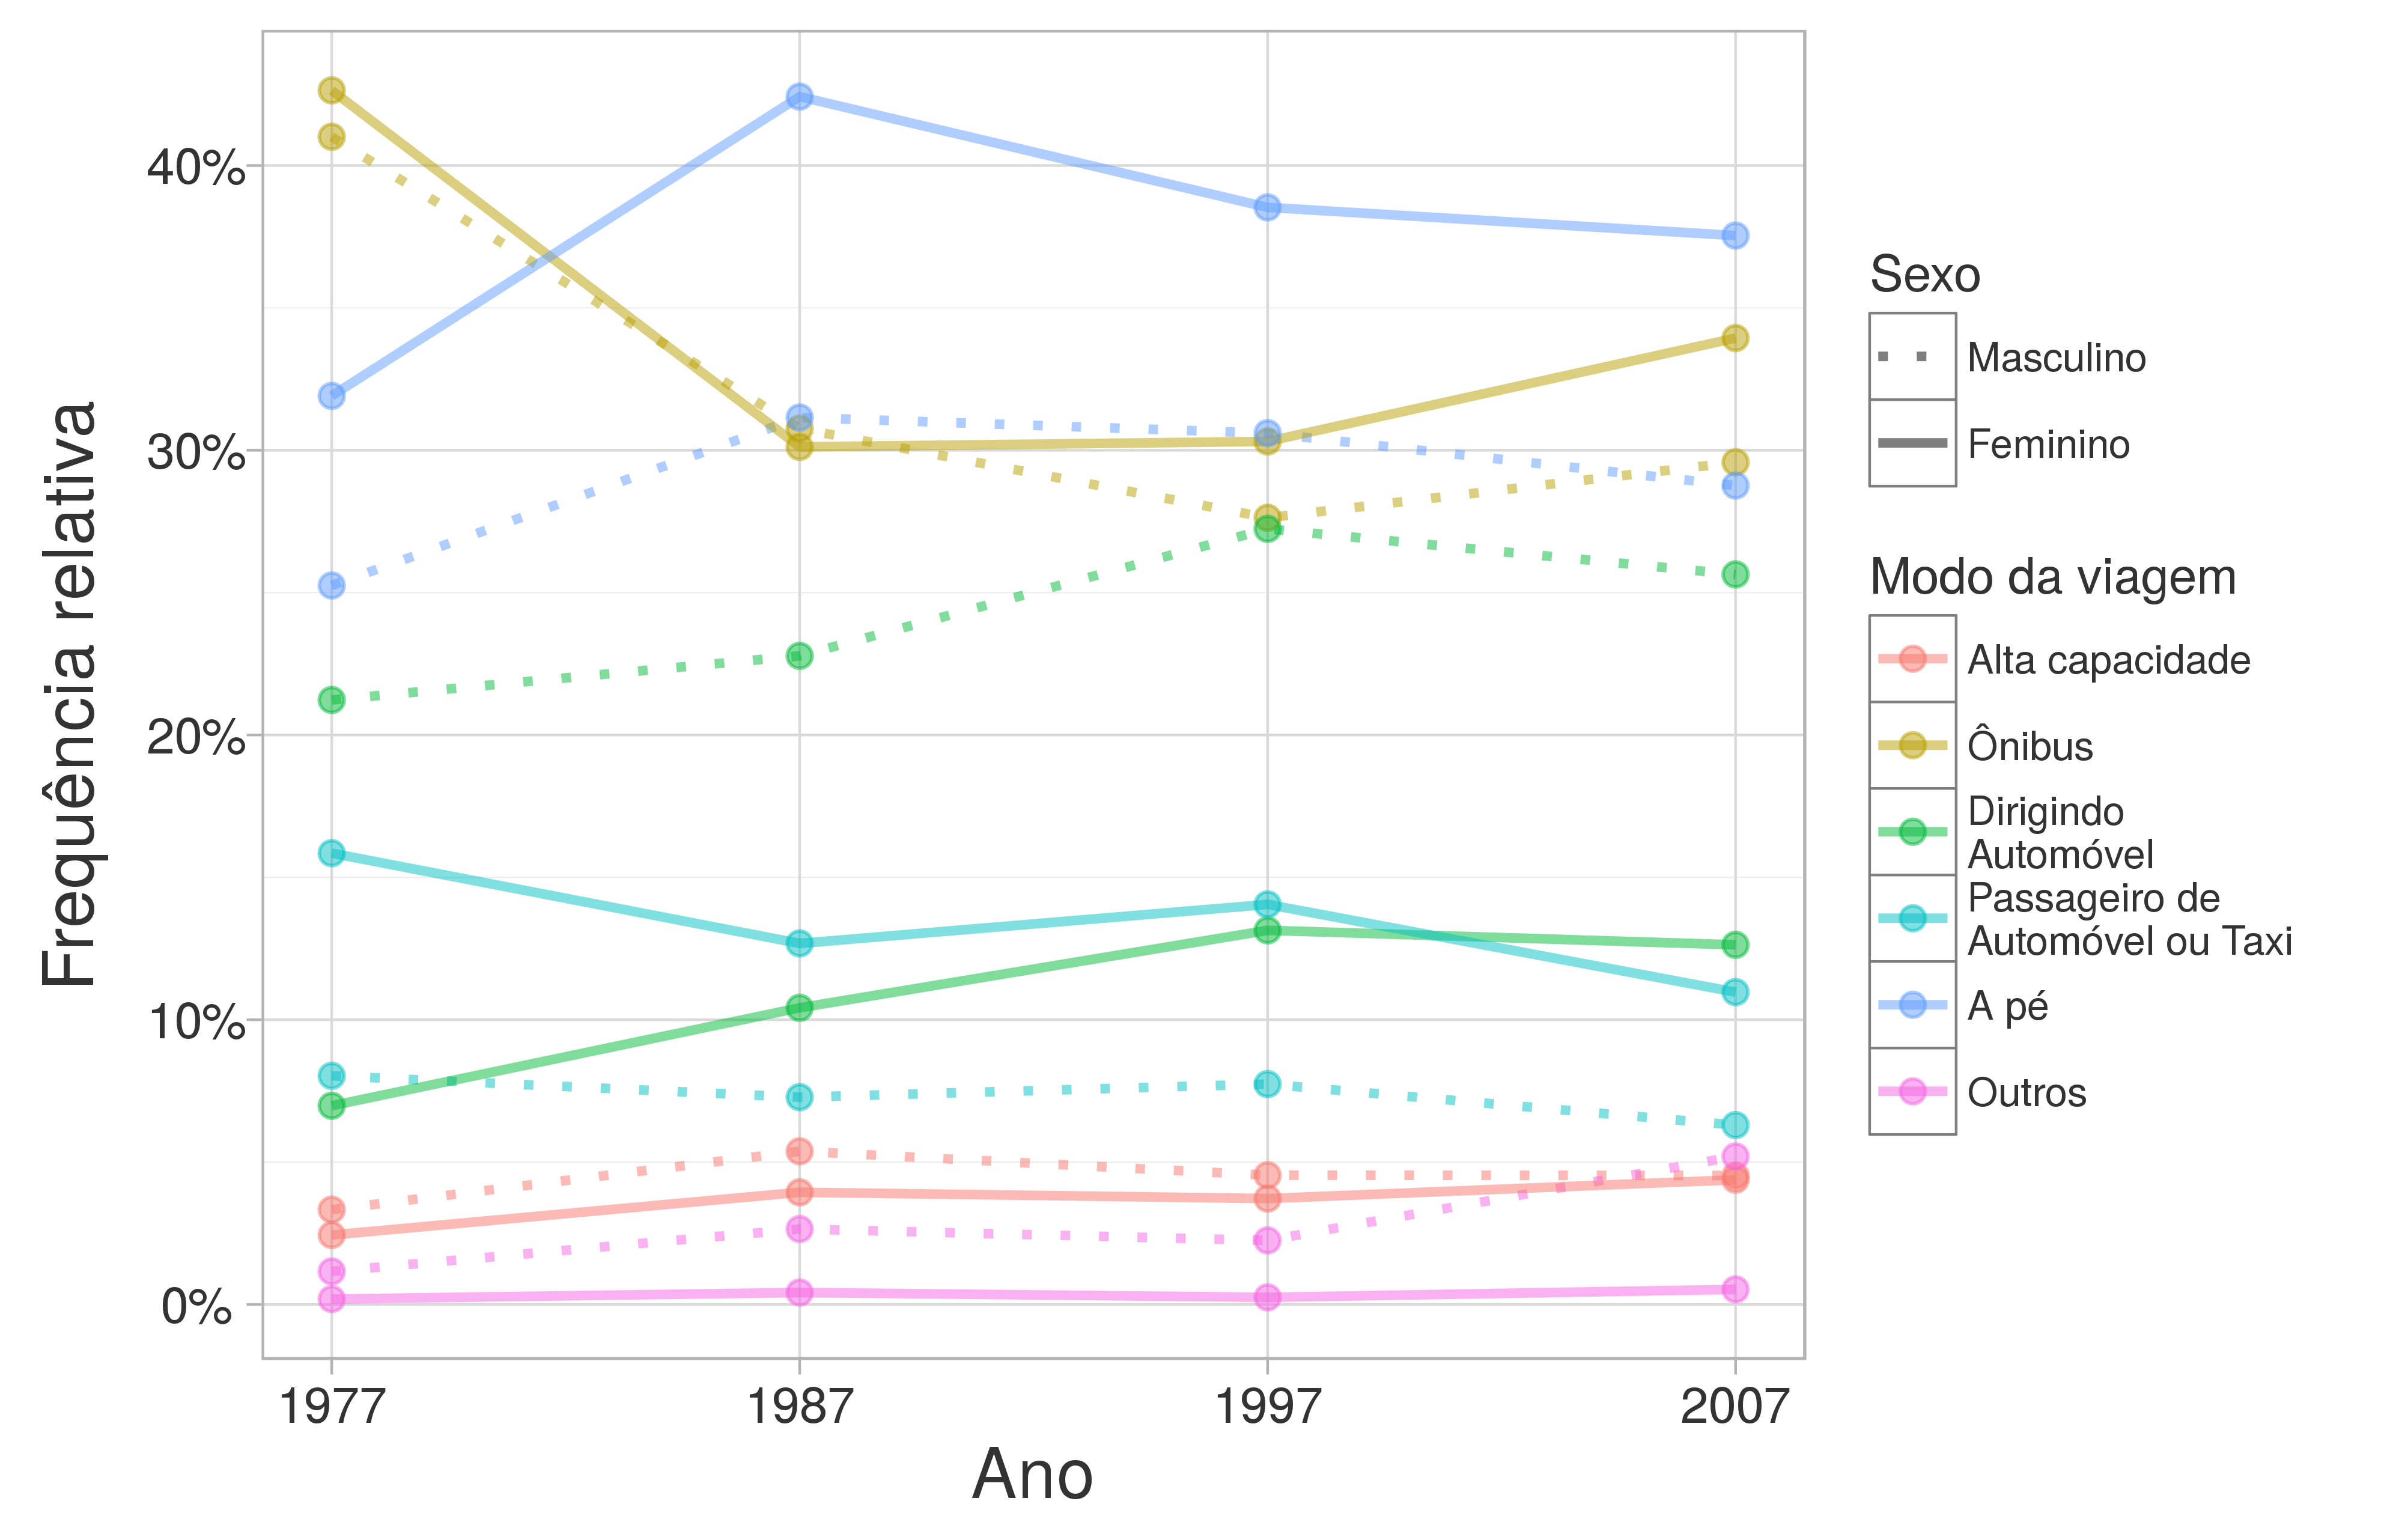
\includegraphics[width=1\textwidth]{./imagens/freq-modo1.png}%
    \end{center}%
%    \fonte{Compilação própria}
\end{grafico}%
% Estatísticas para registros com F_VIAG==1 e SEXO
% Expandido com FE_VIAG

Analisando agora as categorias do segundo modo, por sexo:
\begin{compactitem}[]
\item (i)  As duas categorias que apresentam relevância como segundo modo de transporte são os modos coletivos ônibus e alta capacidade (metrô e trem); os demais ou não foram considerados (por exemplo, a pé) ou não são muito significativos (automóvel e outros).
\item (ii) A utilização feminina do ônibus, como segundo modo da viagem, é inferior à masculina entre 1977 e 1997, ao contrário do que ocorria com o primeiro modo. Em 2007 a situação se altera, quando pessoas do sexo feminino passam a utilizar mais frequentemente o ônibus.
\item (iii) A frequência do uso de alta capacidade é mais expressiva no conjunto do modo 2, embora ainda seja menor que a do ônibus em todos os anos e para ambos sexos.
\item(iv) Para as mulheres, de 1977 para 1987, parece ter havido uma troca modal no segundo modo: houve queda de $\sim$ 1\% no uso do ônibus e aumento também de $\sim$ 1\% no uso de alta capacidade. Foi nesse período em que houve a primeira expansão da rede metro-ferroviária para a zona leste (trecho Sé-Penha).
\end{compactitem}

\begin{grafico}[htb]%
    \caption{\label{graf:freq-modo2}Proporção das viagens do sexo feminino e do sexo masculino, de acordo com o segundo modo da viagem, por ano}%
    \begin{center}%
        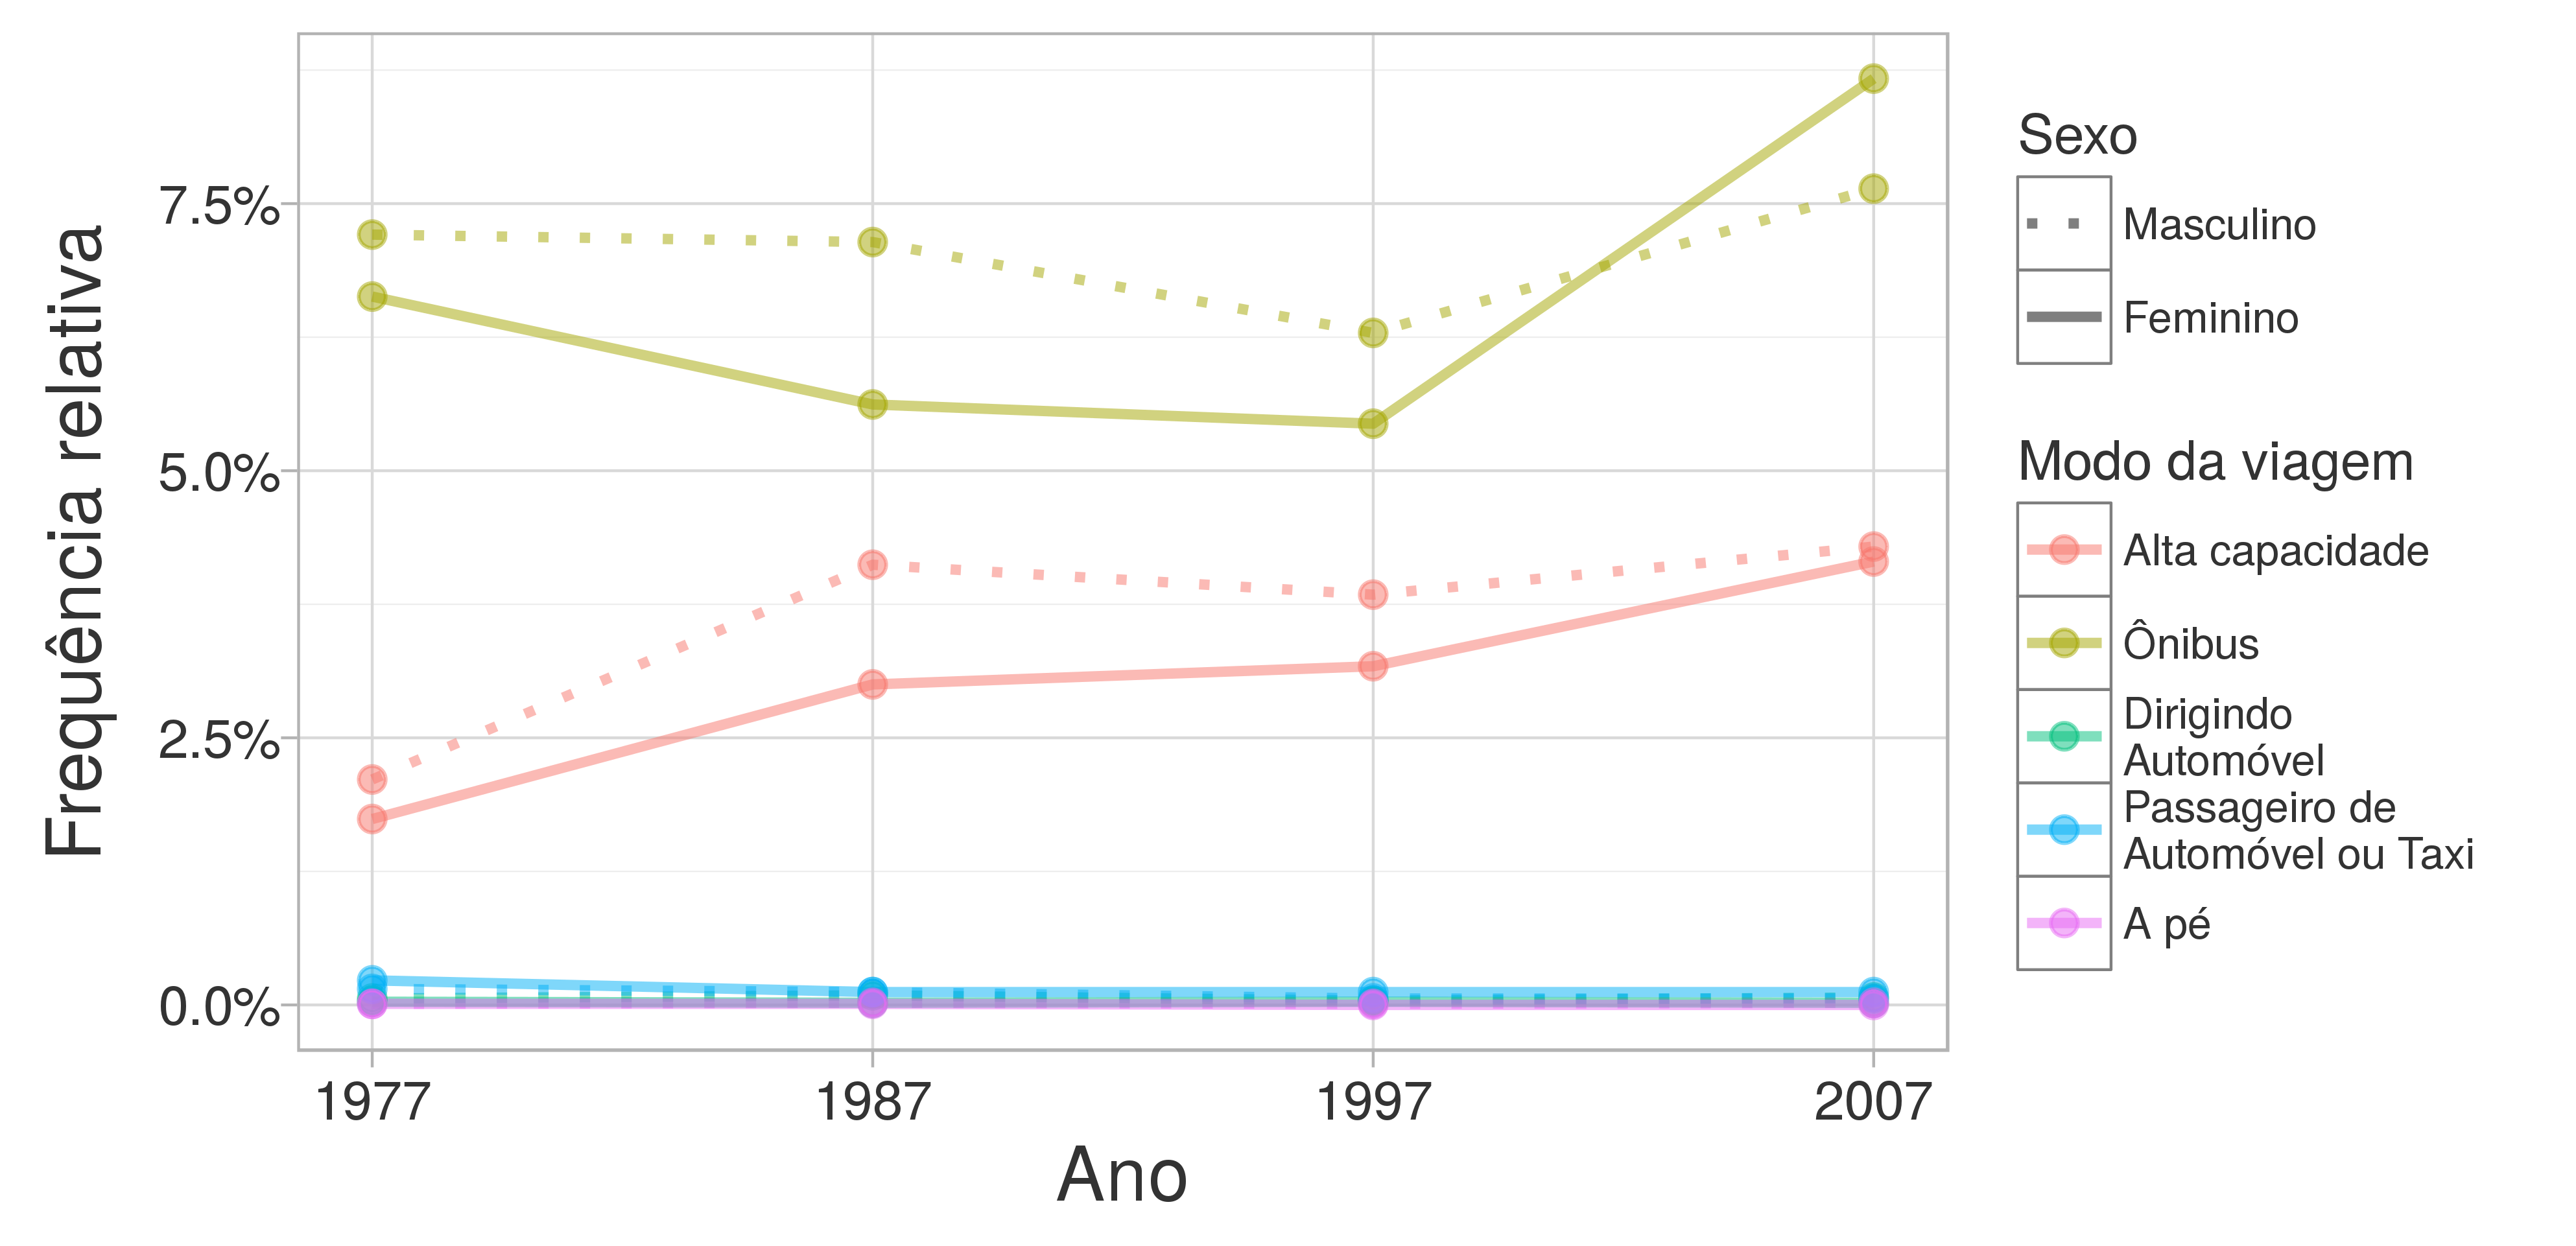
\includegraphics[width=1\textwidth]{./imagens/freq-modo2.png}%
    \end{center}%
%    \fonte{Compilação própria}
\end{grafico}%
% Estatísticas para registros com F_VIAG==1 e SEXO
% Expandido com FE_VIAG

É possível também analisar os modos agregando-os em ``coletivo'', ``individual'' e ``a pé'', o que já fora feito na variável \textbf{TIPO_VIAG}, cujas frequências relativas são apresentadas na Tabela \ref{tab:estat-tipo-viag}.
O transporte individual cresceu de 1977 a 1997 e recuou um pouco em 2007.
O transporte coletivo decresceu entre 1977 e 1987, mas a uma taxa bem maior que o crescimento do individual, o que significa que essas viagens deixaram de ser feitas de transporte coletivo para, principalmente, serem feitas a pé ou, com menor frequência, de carro.
Entre 1987 a 1997 tanto o transporte coletivo como o modo a pé sofrem ligeiras quedas (em torno de 2 pontos percentuais), período em que o transporte individual aumenta sua taxa de crescimento. Neste ano o cenário da divisão modal fica quase equitativamente dividido com cerca de um terço para cada uma das três categorias.
Em 2007 a forma de deslocamento a pé sofre ligeira queda ($\sim$ 1\%), o transporte individual também cai ($\sim$ 2,5\%) e essas viagens passam a ser feitas pelo transporte coletivo que assume proporção um pouco superior à que tinha em 1987.

\begin{table}[htb]
\centering
   \IBGEtab{%\renewcommand{\arraystretch}{1.5}%%\ABNTEXfontereduzida%
        \renewcommand{\arraystretch}{1.5}
        \caption{Frequência relativa da variável \mbox{``TIPO_VIAG''}, por ano}
        \label{tab:estat-tipo-viag}
    }{%

    \begin{tabular}{P{2cm}P{2cm}P{2cm}P{2cm}}
        \toprule
        \textbf{ANO}   & \textbf{Coletivo} & \textbf{Individual} & \textbf{A pé} \\ \midrule \midrule
        \textbf{1977}  & 45,0\%            & 27,0\%              & 28,0\%  \\ \hline
        \textbf{1987}  & 35,6\%            & 28,2\%              & 36,2\%  \\ \hline
        \textbf{1997}  & 33,3\%            & 32,3\%              & 34,4\%  \\ \hline
        \textbf{2007}  & 36,5\%            & 29,5\%              & 33,1\%  \\ \bottomrule          
    \end{tabular}
    }{%
%		\fonte{Elaboração própria}
	}
\end{table}
% Estatísticas para registros com F_VIAG==1
% Expandido com FE_VIAG

O Gráfico \ref{graf:freq-tipo-viag} apresenta a segmentação por sexo do modo (agregado) de viagem.
Comparando ambos os sexos por categoria do primeiro modo:
\begin{compactitem}[]
\item (i) Em 1977, 45,4\% das mulheres usavam o transporte coletivo, 31,9\% deslocavam-se a pé e 22,7\% usavam transporte individual. Em 1987, para elas, o transporte individual permanece no mesmo patamar ($\sim$ 23,2\%) e ocorre uma migração do coletivo para o a pé com 34,4\% e 42,4\%, respectivamente.
\item (ii) Em 1977, 44,7\% dos homens usavam o transporte coletivo, 30,1\% o individual e 25,3\% deslocavam-se a pé. Em 1987, para eles, o transporte individual cresceu ($\sim$ 32,3\%) e as viagens a pé também ($\sim$ 31,2\%) indicando uma migração do transporte coletivo (36,5\%) para estes modos.
\item (iii) Entre 1987 e 1997, a proporção de mulheres a usar o transporte coletivo permanece inalterada, mas ocorre uma migração do modo a pé para o transporte individual.
\item (iv) Entre 1987 e 1997, a proporção de homens a usar o transporte individual continua aumentando (para 37\%), superando a participação do coletivo (32,4\%), enquanto as viagens a pé permanecem no mesmo patamar.
\item (v) Entre 1997 e 2007, a proporção do uso feminino do transporte coletivo cresce (para 38,7\%) indicando migração para este modo das viagens advindas, especialmente, do transporte individual (que cai para 23,6\%) e, em menor medida, do modo a pé (com 37,5\%). 
\item (vi) Entre 1997 e 2007, a proporção do uso masculino do transporte coletivo também cresce (para 34,4\%) indicando migração para este modo das viagens advindas tanto do transporte individual (que cai para 35,4\%) como do modo a pé (com 28,8\%).
\end{compactitem}
% Em 2007 não fecha 100% porque havia no banco uns casos de TIPO_VIAG=4, cujo significado desconheço pois valor não consta do layout

\begin{grafico}[htb]%
    \caption{\label{graf:freq-tipo-viag}Proporção das viagens do sexo feminino e do sexo masculino, segundo o modo da viagem (agregado), por ano}%
    \begin{center}%
        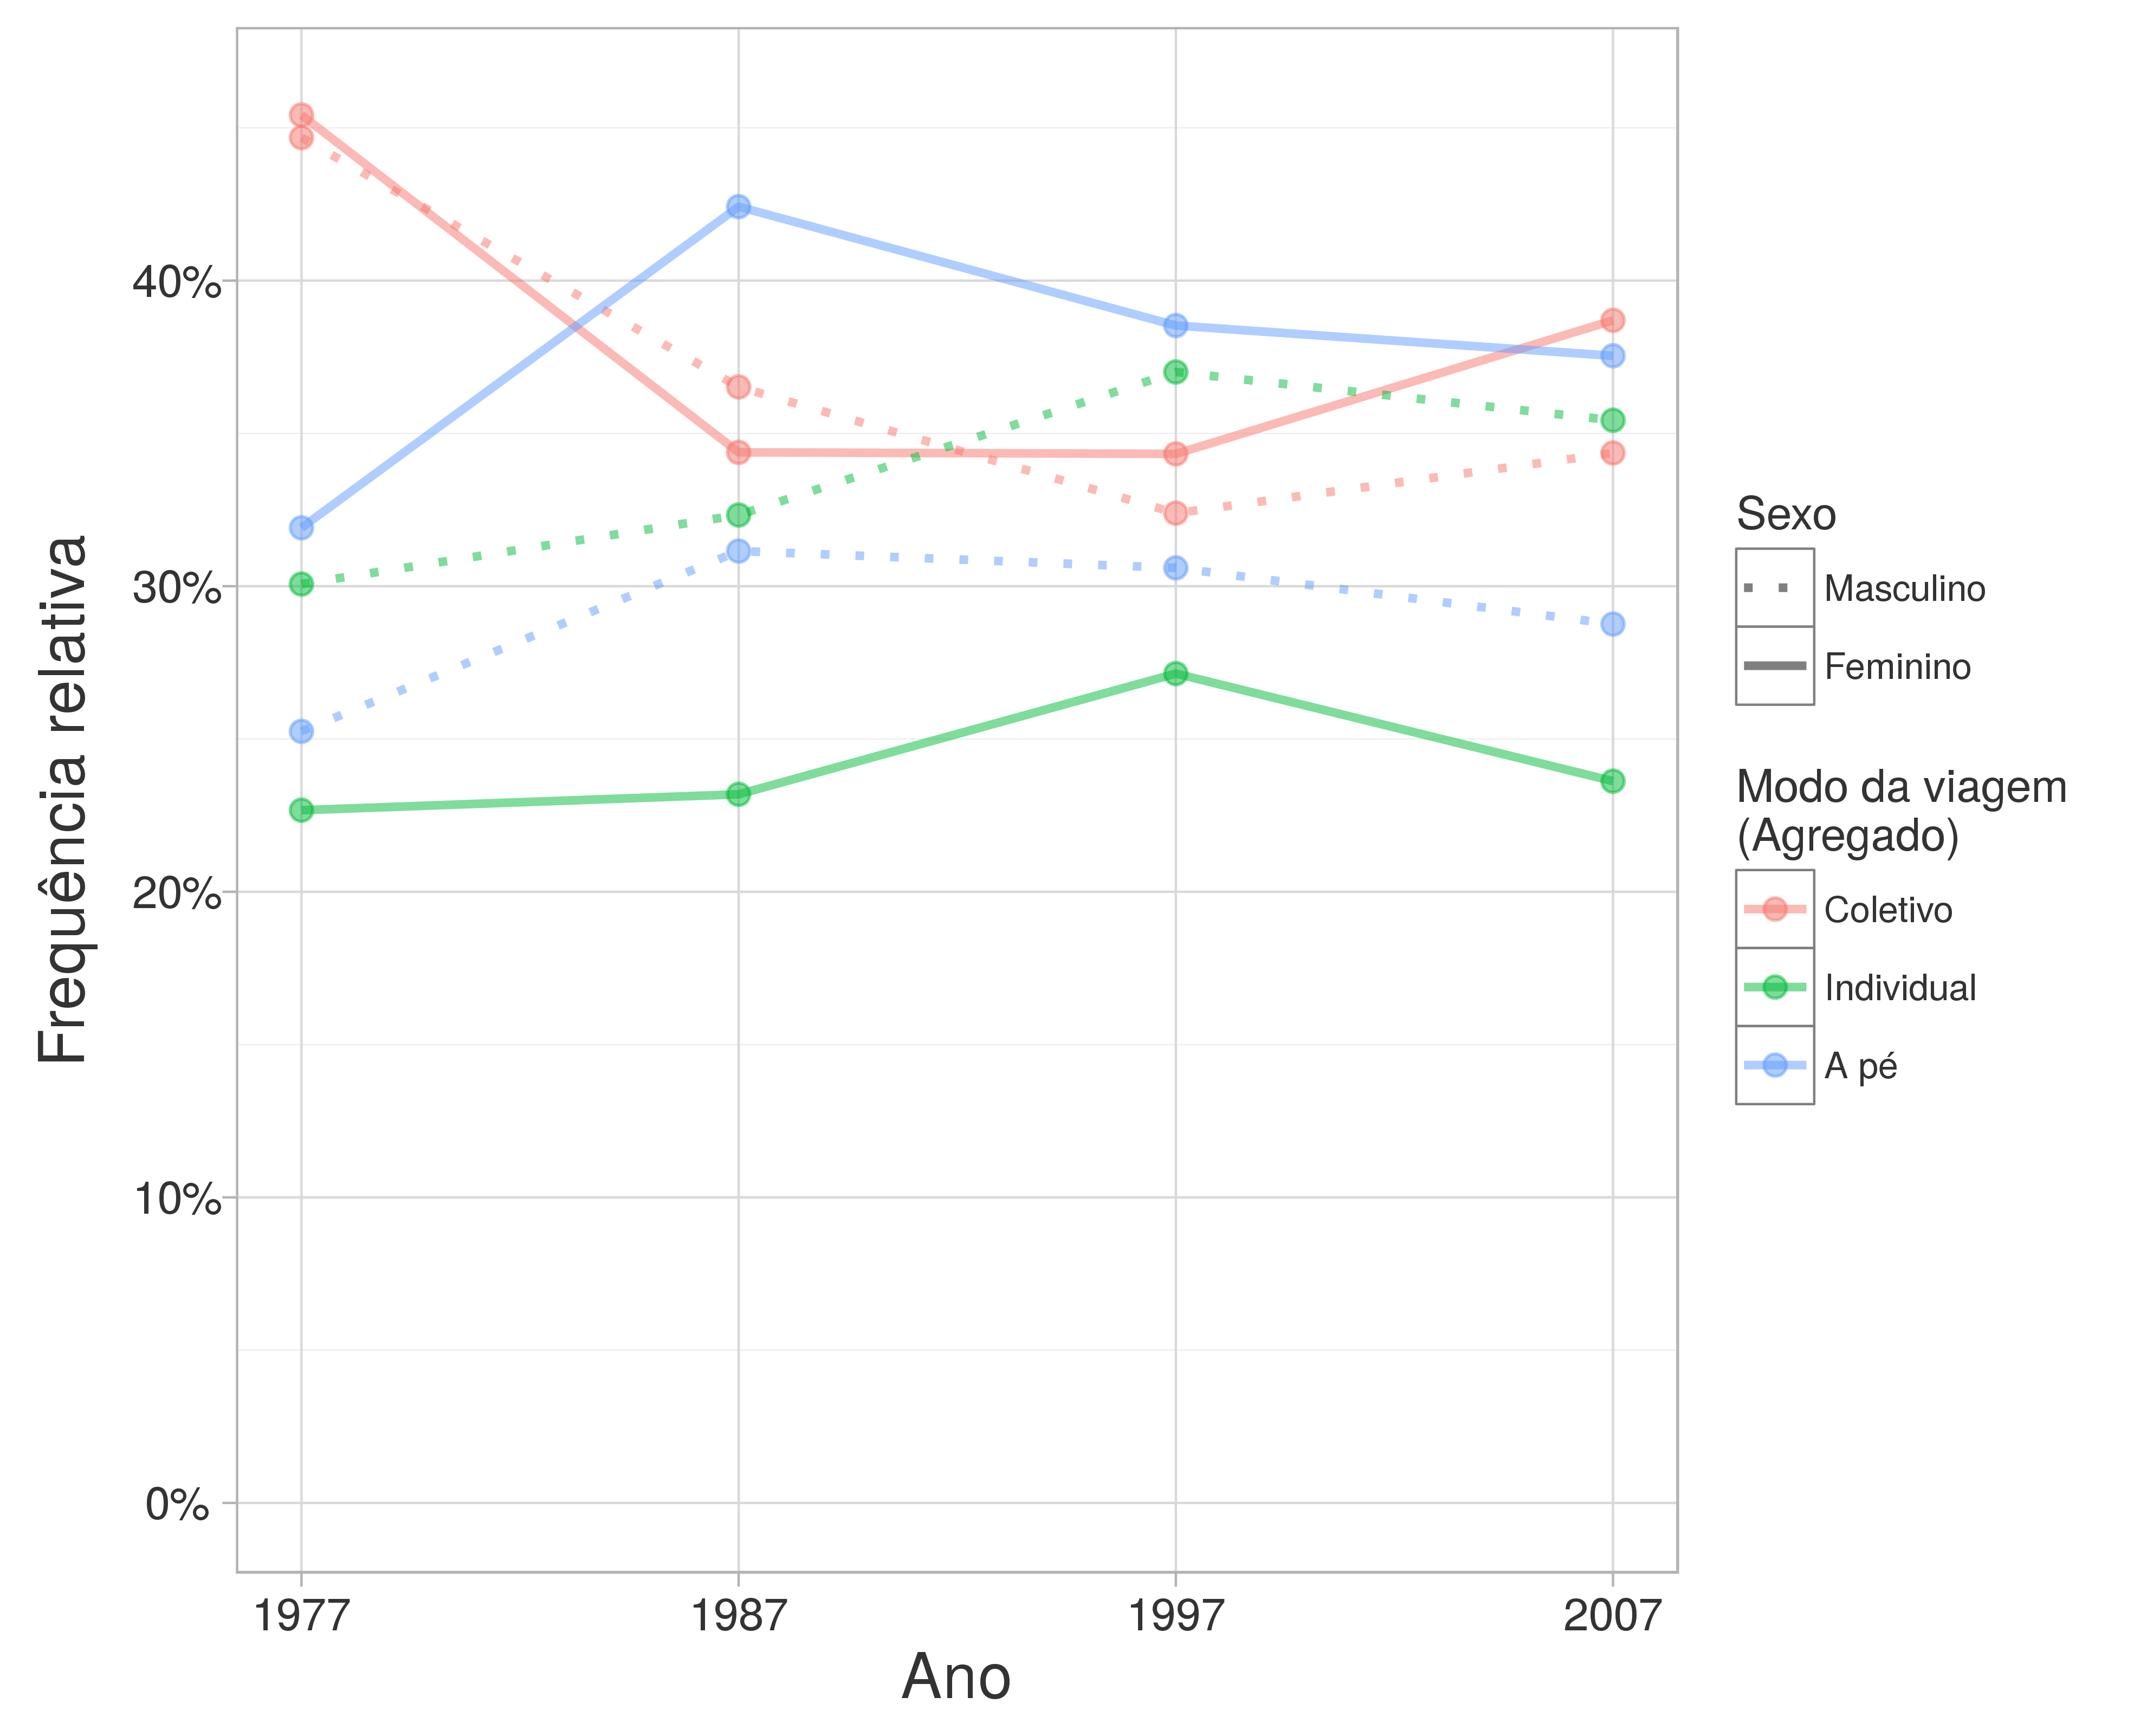
\includegraphics[width=1\textwidth]{./imagens/freq-tipo-viag.png}%
    \end{center}%
%    \fonte{Compilação própria}
\end{grafico}%
% Estatísticas para registros com F_VIAG==1 e SEXO
% Expandido com FE_VIAG

Para as variáveis de motivo (\textbf{MOTIVO_ORIG} e \textbf{MOTIVO_DEST}) foi criada a categoria ``servir passageiro''. Para tanto, olhava-se a variável ``servir passageiro no destino'' de cada pesquisa OD; caso fosse afirmativo (1), a categoria adotada é ``servir passageiro'', porque o que motiva esse deslocamento é o motivo de outrem, não o da pessoa respondente. Caso contrário, adota-se o motivo de origem indicado originalmente na base de dados. Tal procedimento foi realizado com as bases de 1997 e 2007. A base de 1977 já conta com a categoria ``servir passageiro''. A base de 1987 é a única que não possui informações suficientes para identificar esse motivo de viagem.

Será explorada a variável motivo no destino porque essa variável indica a atividade fim que gerou o deslocamento.
A Tabela \ref{tab:estat-motivo-dest} foi elaborada expandindo as viagens pelo \mbox{FE_VIAG}, consequentemente foram consideradas apenas as viagens realizadas (cujos \mbox{FE_VIAG} não são iguais a zero).
Observa-se que o motivo ``residência'' corresponde à maior parte das viagens realizadas (cerca de 45\%), se alterando pouco ao longo dos anos - resultado próximo ao esperado (pouco menos de 50\%) dado que o comportamento de deslocamentos da demanda tem a residência como base, ou seja, é para onde a maior parte das pessoas retornam após executar alguma outra atividade.
O segundo motivo mais frequente é ``trabalho'' girando em torno dos 23,5\% e também oscilando pouco (1\%) ao longo dos anos, seguido por ``educação'', que cresce de 1977 (13,2\%) para 1987 (16,9\%) e depois decresce em 1997 (14\%) e se mantém em 2007 (14\%).
Assim, trabalho, educação e residência são os motivos de pouco mais de 80\% das viagens em todos os anos.
A proporção das viagens motivo ``manutenção-compras'' cresce de 1977 (3,9\%) para 1987 (4,5\%) e praticamente retorna ao mesmo patamar em 1997 (3,8\%), caindo um mais um pouco em 2007 (3,6\%).
O percentual de viagens motivo ``lazer/outros'' vem diminuindo com o tempo, cerca de 2 pontos percentuais por década.
O percentual de viagens ``servir passageiro'', por sua vez, vem aumentando com o tempo, saindo de 1,0\% em 1977 para 7,0\% em 2007.

\begin{table}[htb]
\centering
   \IBGEtab{%\renewcommand{\arraystretch}{1.5}%%\ABNTEXfontereduzida%
        \renewcommand{\arraystretch}{1.5}
        \caption{Frequência relativa da variável ``MOTIVO_DEST'', por ano}
        \label{tab:estat-motivo-dest}
    }{%

    \begin{tabular}{ccccccc}
        \toprule
        \textbf{}   & \textbf{Servir} & \textbf{} & \textbf{} & \textbf{} & \textbf{Manutenção/} & \textbf{Lazer/} \\
        \textbf{ANO}   & \textbf{Passageiro} & \textbf{Trabalho} & \textbf{Educação} & \textbf{Residência} & \textbf{compras} & \textbf{Outros} \\ \midrule \midrule
        \textbf{1977}  & 1,0\% & 24,4\% & 13,2\% & 44,6\% & 3,9\% & 12,9\% \\ \hline
        \textbf{1987}  &   -   & 22,6\% & 16,9\% & 45,7\% & 4,5\% & 10,3\% \\ \hline
        \textbf{1997}  & 6,4\% & 22,3\% & 14,0\% & 44,9\% & 3,8\% &  8,6\% \\ \hline
        \textbf{2007}  & 7,0\% & 23,7\% & 14,0\% & 45,0\% & 3,6\% &  6,7\% \\\bottomrule          
      
    \end{tabular}
    }{%
%		\fonte{Elaboração própria}
	}
\end{table}
% Estatísticas para registros com F_VIAG==1
% Expandido com FE_VIAG

%\begin{table}[htb]
%    \IBGEtab{%\renewcommand{\arraystretch}{1.5}%%\ABNTEXfontereduzida%
%        \renewcommand{\arraystretch}{1.5}
%        \caption{Estatísticas da variável ``MOTIVO_DEST''}
%        \label{tab:estat-motivo-dest}
%    }{%
%
%    \begin{tabular}{cccccc}
%        \toprule
%        \textbf{ANO} & \textbf{1977} & \textbf{1987} & \textbf{1997} & \textbf{2007} & \textbf{Total}\\ \midrule \midrule
%        \textbf{MOTIVO_DEST=1}  & 13.688 & 12.629 &  5.663 &  4.434 &  36.414 \\ \hline
%        \textbf{MOTIVO_DEST=2}  &  9.159 &  8.374 &  8.439 &  7.536 &  33.508 \\ \hline
%        \textbf{MOTIVO_DEST=3}  & 19.248 & 20.345 & 22.984 & 29.239 &  91.816 \\ \hline
%        \textbf{MOTIVO_DEST=4}  & 26.363 & 31.161 & 28.970 & 27.589 & 114.083 \\ \hline
%        \textbf{MOTIVO_DEST=5}  &  4.310 &  4.618 &  4.166 &  4.652 &  17.746 \\ \hline
%        \textbf{MOTIVO_DEST=6}  &  2.675 &  3.464 &  3.391 &  3.954 &  13.484 \\ \hline
%        \textbf{MOTIVO_DEST=7}  & 11.940 & 10.306 &  6.465 &  5.419 &  34.130 \\ \hline
%        \textbf{MOTIVO_DEST=8}  & 83.660 & 83.720 & 73.315 & 75.217 & 315.912 \\ \hline
%        \textbf{MOTIVO_DEST=9}  & 16.374 &  8.501 & 10.141 & 11.625 &  46.641 \\ \hline
%        \textbf{MOTIVO_DEST=NA} &     24 &      0 &      0 &      0 &      24 \\ \bottomrule
%        \end{tabular}
%    }
%
%\end{table}
%% Estatísticas para registros com F_VIAG==1

Ao observar o Gráfico \ref{graf:freq-motivos}, que dentro de cada ano segmenta por sexo os motivos de viagens, percebe-se que as proporções das viagens motivo ``trabalho'' femininas são sempre inferiores às masculinas e essa diferença vem diminuindo com o tempo por conta da maior participação das mulheres no mercado de trabalho.
As proporções das viagens motivo ``educação'' femininas são sempre superiores às masculinas e essa diferença vem diminuindo, de forma que em 2007 não chega a 1\%.
As viagens motivo ``lazer / outros'' cai em ambos sexos, sendo as porcentagens das viagens femininas superiores às masculinas em todos os períodos.
As viagens motivo ``manutenção / compras'' são sempre mais frequentes para mulheres do que para homens e a diferença entre ambos caiu de 4,05 ponto percentuais em 1977, quando as mulheres faziam 2,8 vezes mais viagens deste tipo do que os homens, para 2,25 pontos percentuais em 2007, quando as mulheres passaram a fazer quase o dobro (1,9 vezes) deste tipo de viagem que os homens.
As viagens motivo ``servir passageiro'' são menos representativas do total para ambos sexos e sempre mais frequentes para mulheres do que para homens. Excluindo 1987, cujos dados não estavam disponíveis nesta categoria, a relação entre o percentual feminino e o masculino era de 2,3  em 1977, passou para 1,8 em 1997 e para 1,5 em 2007.

\begin{grafico}[htb]%
    \caption{\label{graf:freq-motivos}Proporção das viagens do sexo feminino e do sexo masculino, segundo o motivo no destino, por ano}%
    \begin{center}%
        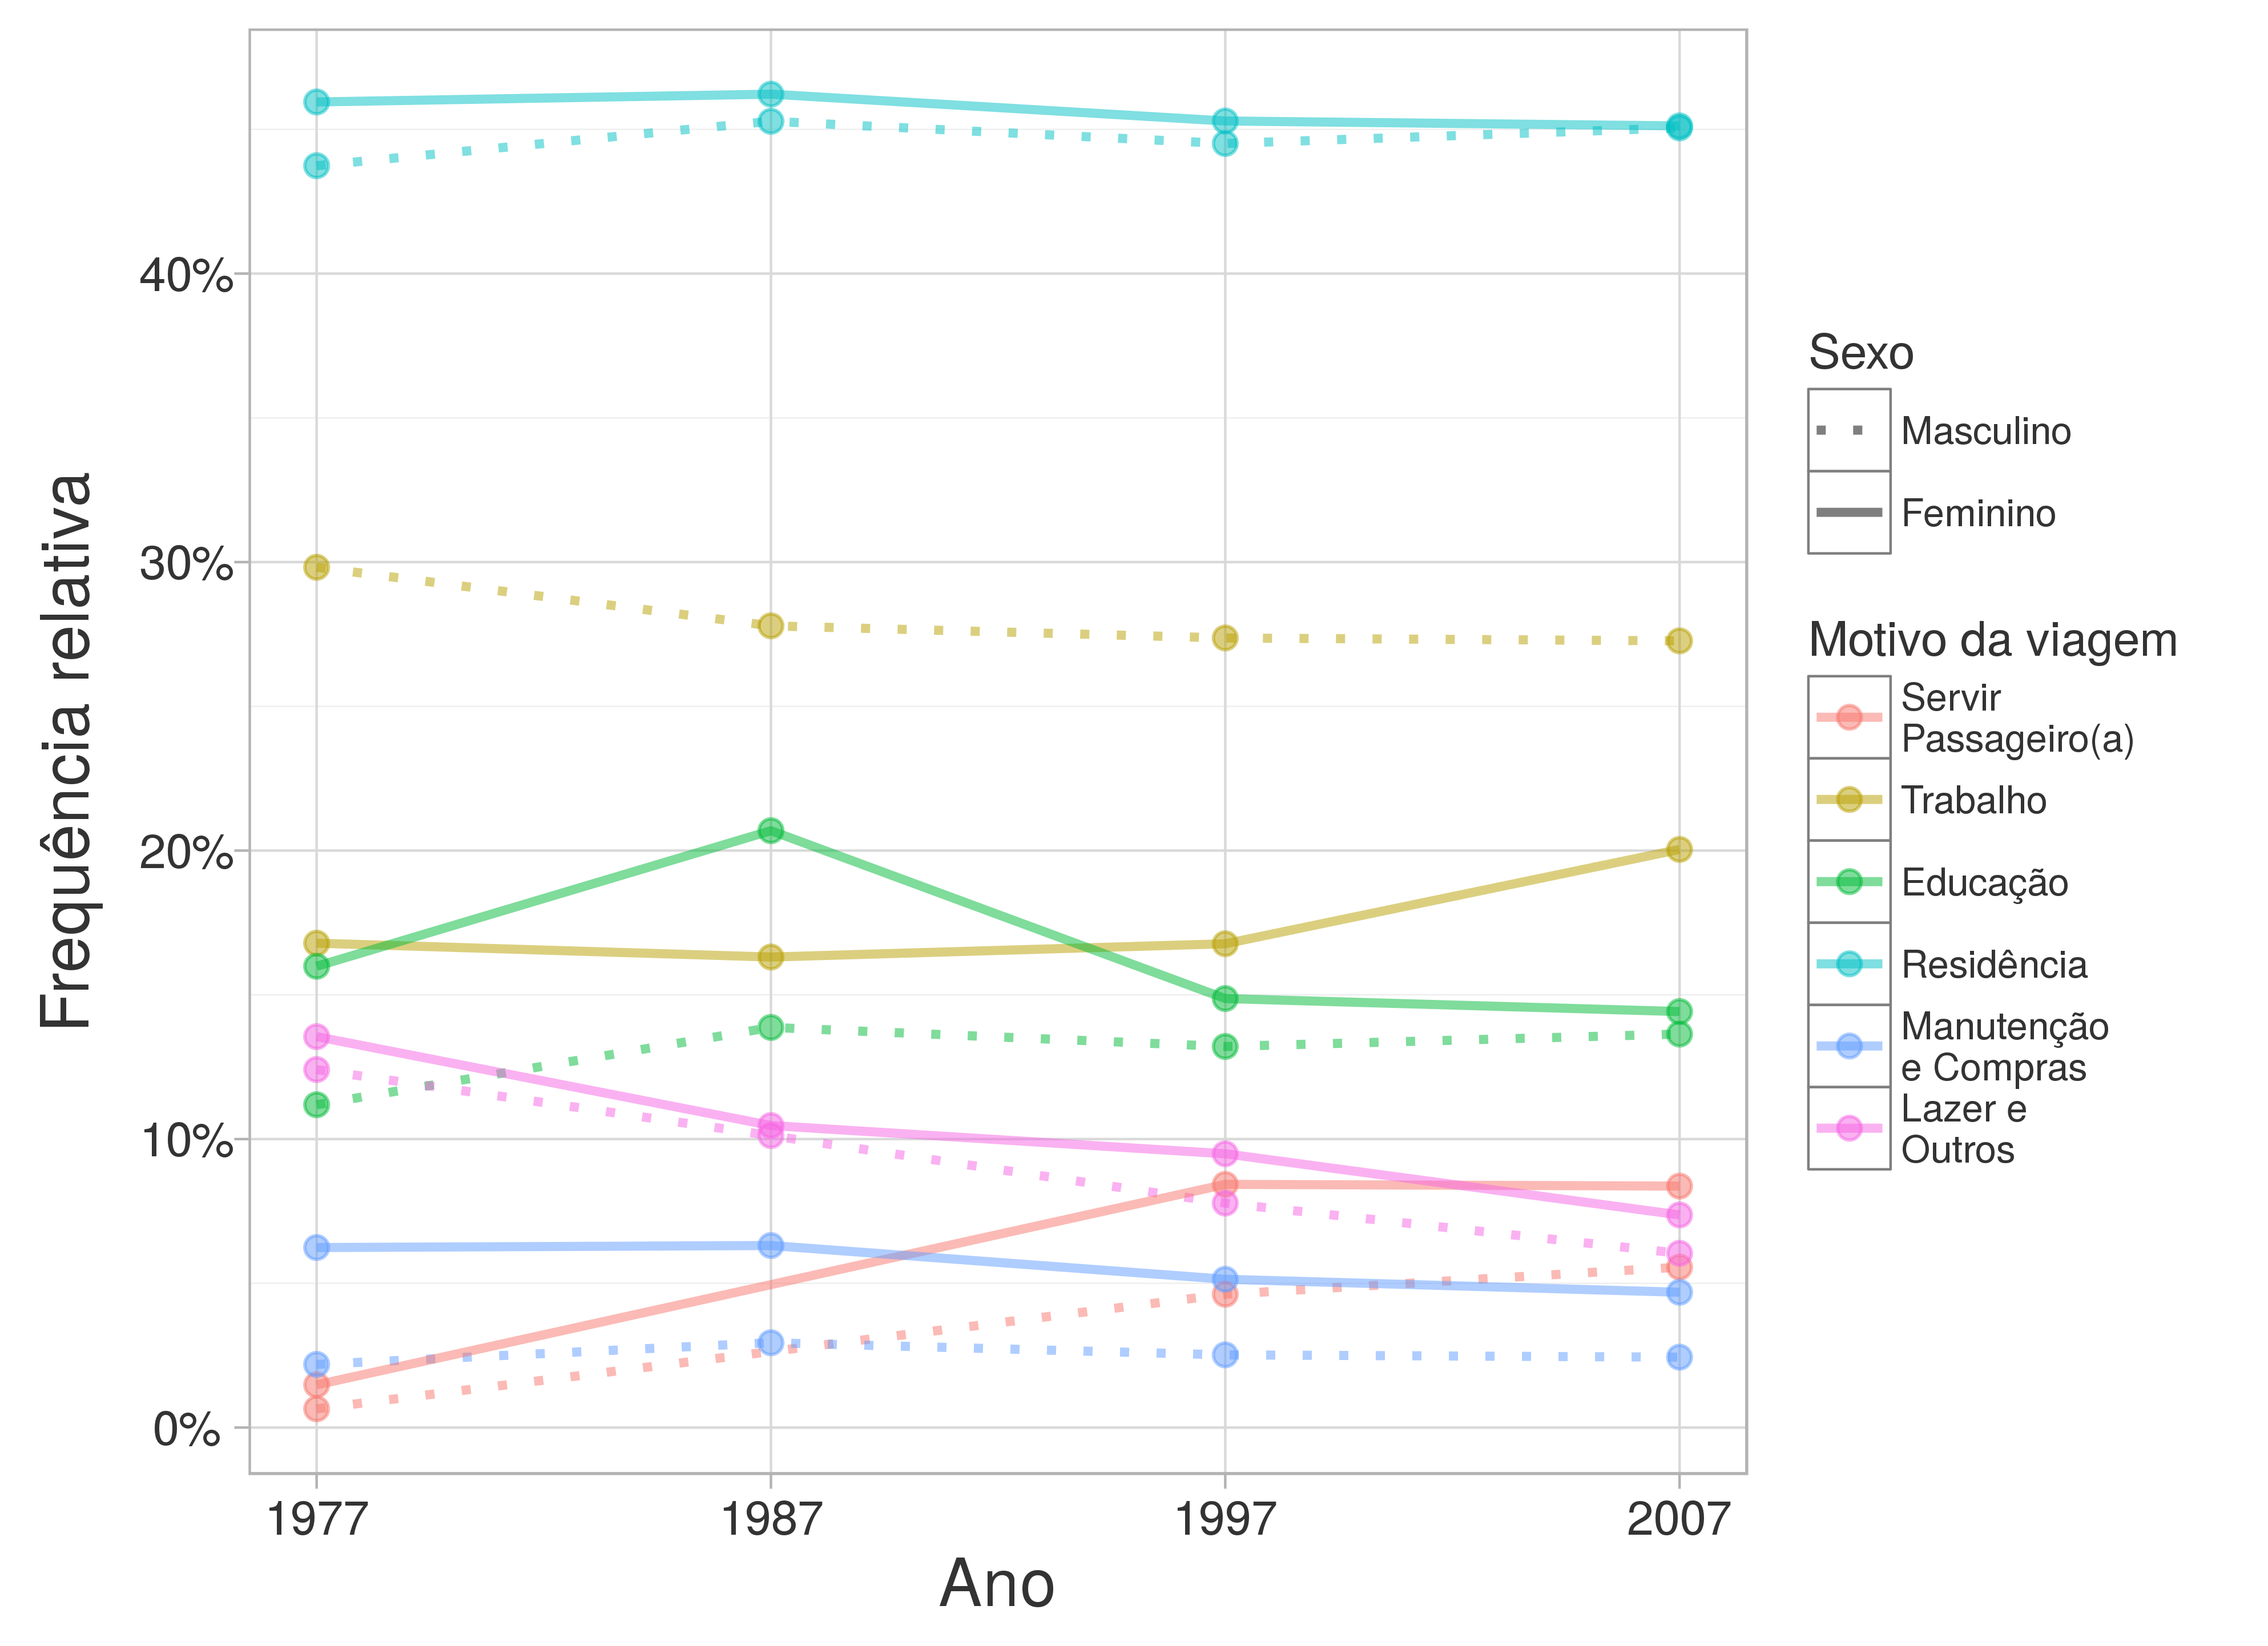
\includegraphics[width=0.9\textwidth]{./imagens/freq-motivo.png}%
    \end{center}%
%    \fonte{Compilação própria}
\end{grafico}%
% Estatísticas para registros com F_VIAG==1 e SEXO
% Expandido com FE_VIAG

%A variável \textbf{DURACAO} representa a duração total da viagem de uma pessoa, a duração média por pessoa é o somatório das durações dividido pelo número total de viagens de cada pessoa.
%Não existem \textit{missing values} neste campo, os valores mínimos para todos anos e ambos sexo são 0, bem como também são 0 os valores do primeiro quartil (25\%). Os valores das demais estatísticas (considerando os fatores de expansão para a população) estão apresentados na Tabela \ref{tab:estat-dur-med-viag}. Conforme já era de se esperar, para quem faz viagem no dia da pesquisa (número de viagem é não nulo) existe a predominância do valor 2, ou seja, são pessoas que saem de suas residências com um propósito único (trabalhar, estudar, fazer compras) e depois retornam à residência após a atividade.
%Percebe-se que, independente do sexo, o número médio de viagens por pessoa em relação a 1977 caiu um pouco em 1987 e 1997 (de 1,67 para 1,64) e subiu novamente em 2007 (para 1,70). Os desvios padrão caíram ao longo do tempo, indicando tendência de menor dispersão dos dados. Os valores de assimetria são positivos, indicando maior concentração à esquerda e cauda longa à direita da distribuição. Os valores de curtose evidenciam não tratar-se de distribuição normal.
%Analisando esses dados segmentados por sexo, vê-se que as medianas são iguais. O número médio e máximo de viagens para mulheres é sempre inferior ao dos homens, para o mesmo ano. Os valores de assimetria para o sexo feminino e o masculino são positivos e convergem para o valor geral com o passar das décadas. 
%A diferença entre o número médio de viagens de mulheres e homens vem diminuindo.

%\begin{table}[htb]
%\centering
%   \IBGEtab{%\renewcommand{\arraystretch}{1.5}%%\ABNTEXfontereduzida%
%        \renewcommand{\arraystretch}{1.5}
%        \caption{Estatísticas da variável ``PESS_DURACAO_MED'', por ano e por sexo}
%        \label{tab:estat-dur-med-viag}
%    }{%
%
%    \begin{tabular}{ccccccc}
%        \toprule
%        \textbf{Geral} & \multicolumn{3}{c}{\textbf{}} & \multicolumn{3}{c}{\textbf{}} \\ \hline
%        \textbf{ANO}   & \textbf{Média} & \textbf{Desvio Padrão} & \textbf{Mediana} & \textbf{Máximo} & \textbf{Assimetria} & \textbf{Curtose} \\ \midrule \midrule
%        \textbf{1977}  & 21,31 & 28,96 & 10,00 & 240 & 2,06 & 5,74 \\ \hline
%        \textbf{1987}  & 22,41 & 30,04 & 10,00 & 360 & 1,95 & 4,68 \\ \hline
%        \textbf{1997}  & 23,22 & 31,07 & 12,50 & 315 & 1,99 & 4,75 \\ \hline
%        \textbf{2007}  & 29,16 & 35,94 & 16,25 & 240 & 1,68 & 2,94 \\\bottomrule          
%
%        \textbf{Sexo Feminino} & \multicolumn{3}{c}{\textbf{}} & \multicolumn{3}{c}{\textbf{}} \\ \hline
%        \textbf{ANO}   & \textbf{Média} & \textbf{Desvio Padrão} & \textbf{Mediana} & \textbf{Máximo} & \textbf{Assimetria} & \textbf{Curtose} \\ \midrule \midrule
%        \textbf{1977}  & 16,49 & 25,70 &  5,00 & 240 & 1,80 & 4,41 \\ \hline
%        \textbf{1987}  & 17,55 & 26,68 &  5,00 & 360 & 1,66 & 3,16 \\ \hline
%        \textbf{1997}  & 19,89 & 28,67 & 10,00 & 300 & 1,82 & 3,93 \\ \hline
%        \textbf{2007}  & 26,49 & 34,93 & 15,00 & 240 & 1,55 & 2,45 \\\bottomrule
%        
%        \textbf{Sexo Masculino} & \multicolumn{3}{c}{\textbf{}} & \multicolumn{3}{c}{\textbf{}} \\ \hline
%        \textbf{ANO}   & \textbf{Média} & \textbf{Desvio Padrão} & \textbf{Mediana} & \textbf{Máximo} & \textbf{Assimetria} & \textbf{Curtose} \\ \midrule \midrule
%        \textbf{1977}  & 26,39 & 31,24 & 16,67 & 240 & 2,41 & 7,94 \\ \hline
%        \textbf{1987}  & 26,80 & 32,49 & 16,67 & 310 & 2,32 & 7,22 \\ \hline
%        \textbf{1997}  & 27,66 & 33,09 & 15,00 & 315 & 2,17 & 5,71 \\ \hline
%        \textbf{2007}  & 32,13 & 36,81 & 20,00 & 240 & 1,82 & 3,54 \\\bottomrule             
%       
%    \end{tabular}
%    }{%
%%		\fonte{Elaboração própria}
%	}
%\end{table}
%% Estatísticas para registros com F_PESS==1, filtro por SEXO
%% Expandido com FE_PESS
%
%\begin{table}[htb]
%\centering
%   \IBGEtab{%\renewcommand{\arraystretch}{1.5}%%\ABNTEXfontereduzida%
%        \renewcommand{\arraystretch}{1.5}
%        \caption{Estatísticas da variável ``PESS_DURACAO_MED'', por ano e por sexo, considerando somente quem fez viagem com duração superior a 4 minutos}
%        \label{tab:estat-dur-med-viag-maisde4}
%    }{%
%
%    \begin{tabular}{ccccccc}
%        \toprule
%        \textbf{Geral} & \multicolumn{3}{c}{\textbf{}} & \multicolumn{3}{c}{\textbf{}} \\ \hline
%        \textbf{ANO}   & \textbf{Média} & \textbf{Desvio Padrão} & \textbf{Mediana} & \textbf{Máximo} & \textbf{Assimetria} & \textbf{Curtose} \\ \midrule \midrule
%        \textbf{1977}  & 35,50 & 29,92 & 27,50 & 240 & 1,83 & 4,76 \\ \hline
%        \textbf{1987}  & 36,00 & 31,02 & 26,25 & 360 & 1,67 & 3,58 \\ \hline
%        \textbf{1997}  & 36,90 & 32,11 & 26,67 & 315 & 1,73 & 3,57 \\ \hline
%        \textbf{2007}  & 43,05 & 36,20 & 30,00 & 240 & 1,47 & 2,16 \\\bottomrule          
%
%        \textbf{Sexo Feminino} & \multicolumn{3}{c}{\textbf{}} & \multicolumn{3}{c}{\textbf{}} \\ \hline
%        \textbf{ANO}   & \textbf{Média} & \textbf{Desvio Padrão} & \textbf{Mediana} & \textbf{Máximo} & \textbf{Assimetria} & \textbf{Curtose} \\ \midrule \midrule
%        \textbf{1977}  & 32,39 & 28,00 & 23,33 & 235 & 1,97 & 5,64 \\ \hline
%        \textbf{1987}  & 33,48 & 28,88 & 22,50 & 360 & 1,88 & 5,10 \\ \hline
%        \textbf{1997}  & 34,48 & 30,39 & 25,00 & 300 & 1,82 & 3,90 \\ \hline
%        \textbf{2007}  & 41,79 & 35,87 & 30,00 & 240 & 1,53 & 2,37 \\\bottomrule
%        
%        \textbf{Sexo Masculino} & \multicolumn{3}{c}{\textbf{}} & \multicolumn{3}{c}{\textbf{}} \\ \hline
%        \textbf{ANO}   & \textbf{Média} & \textbf{Desvio Padrão} & \textbf{Mediana} & \textbf{Máximo} & \textbf{Assimetria} & \textbf{Curtose} \\ \midrule \midrule
%        \textbf{1977}  & 37,89 & 31,10 & 30,00 & 240 & 1,73 & 4,22 \\ \hline
%        \textbf{1987}  & 38,89 & 32,39 & 30,00 & 310 & 1,52 & 2,71 \\ \hline
%        \textbf{1997}  & 39,10 & 33,44 & 30,00 & 315 & 1,65 & 3,25 \\ \hline
%        \textbf{2007}  & 44,27 & 36,48 & 30,00 & 240 & 1,42 & 1,99 \\\bottomrule             
%       
%    \end{tabular}
%    }{%
%%		\fonte{Elaboração própria}
%	}
%\end{table}
%% Estatísticas para registros com F_PESS==1, filtro por SEXO
%% Expandido com FE_PESS

%\begin{grafico}[htb]%
%    \caption{\label{graf:distr-duracao}Distribuição da variável ``PESS_DURACAO_MED'' por ano e por sexo}%
%    \begin{center}%
%        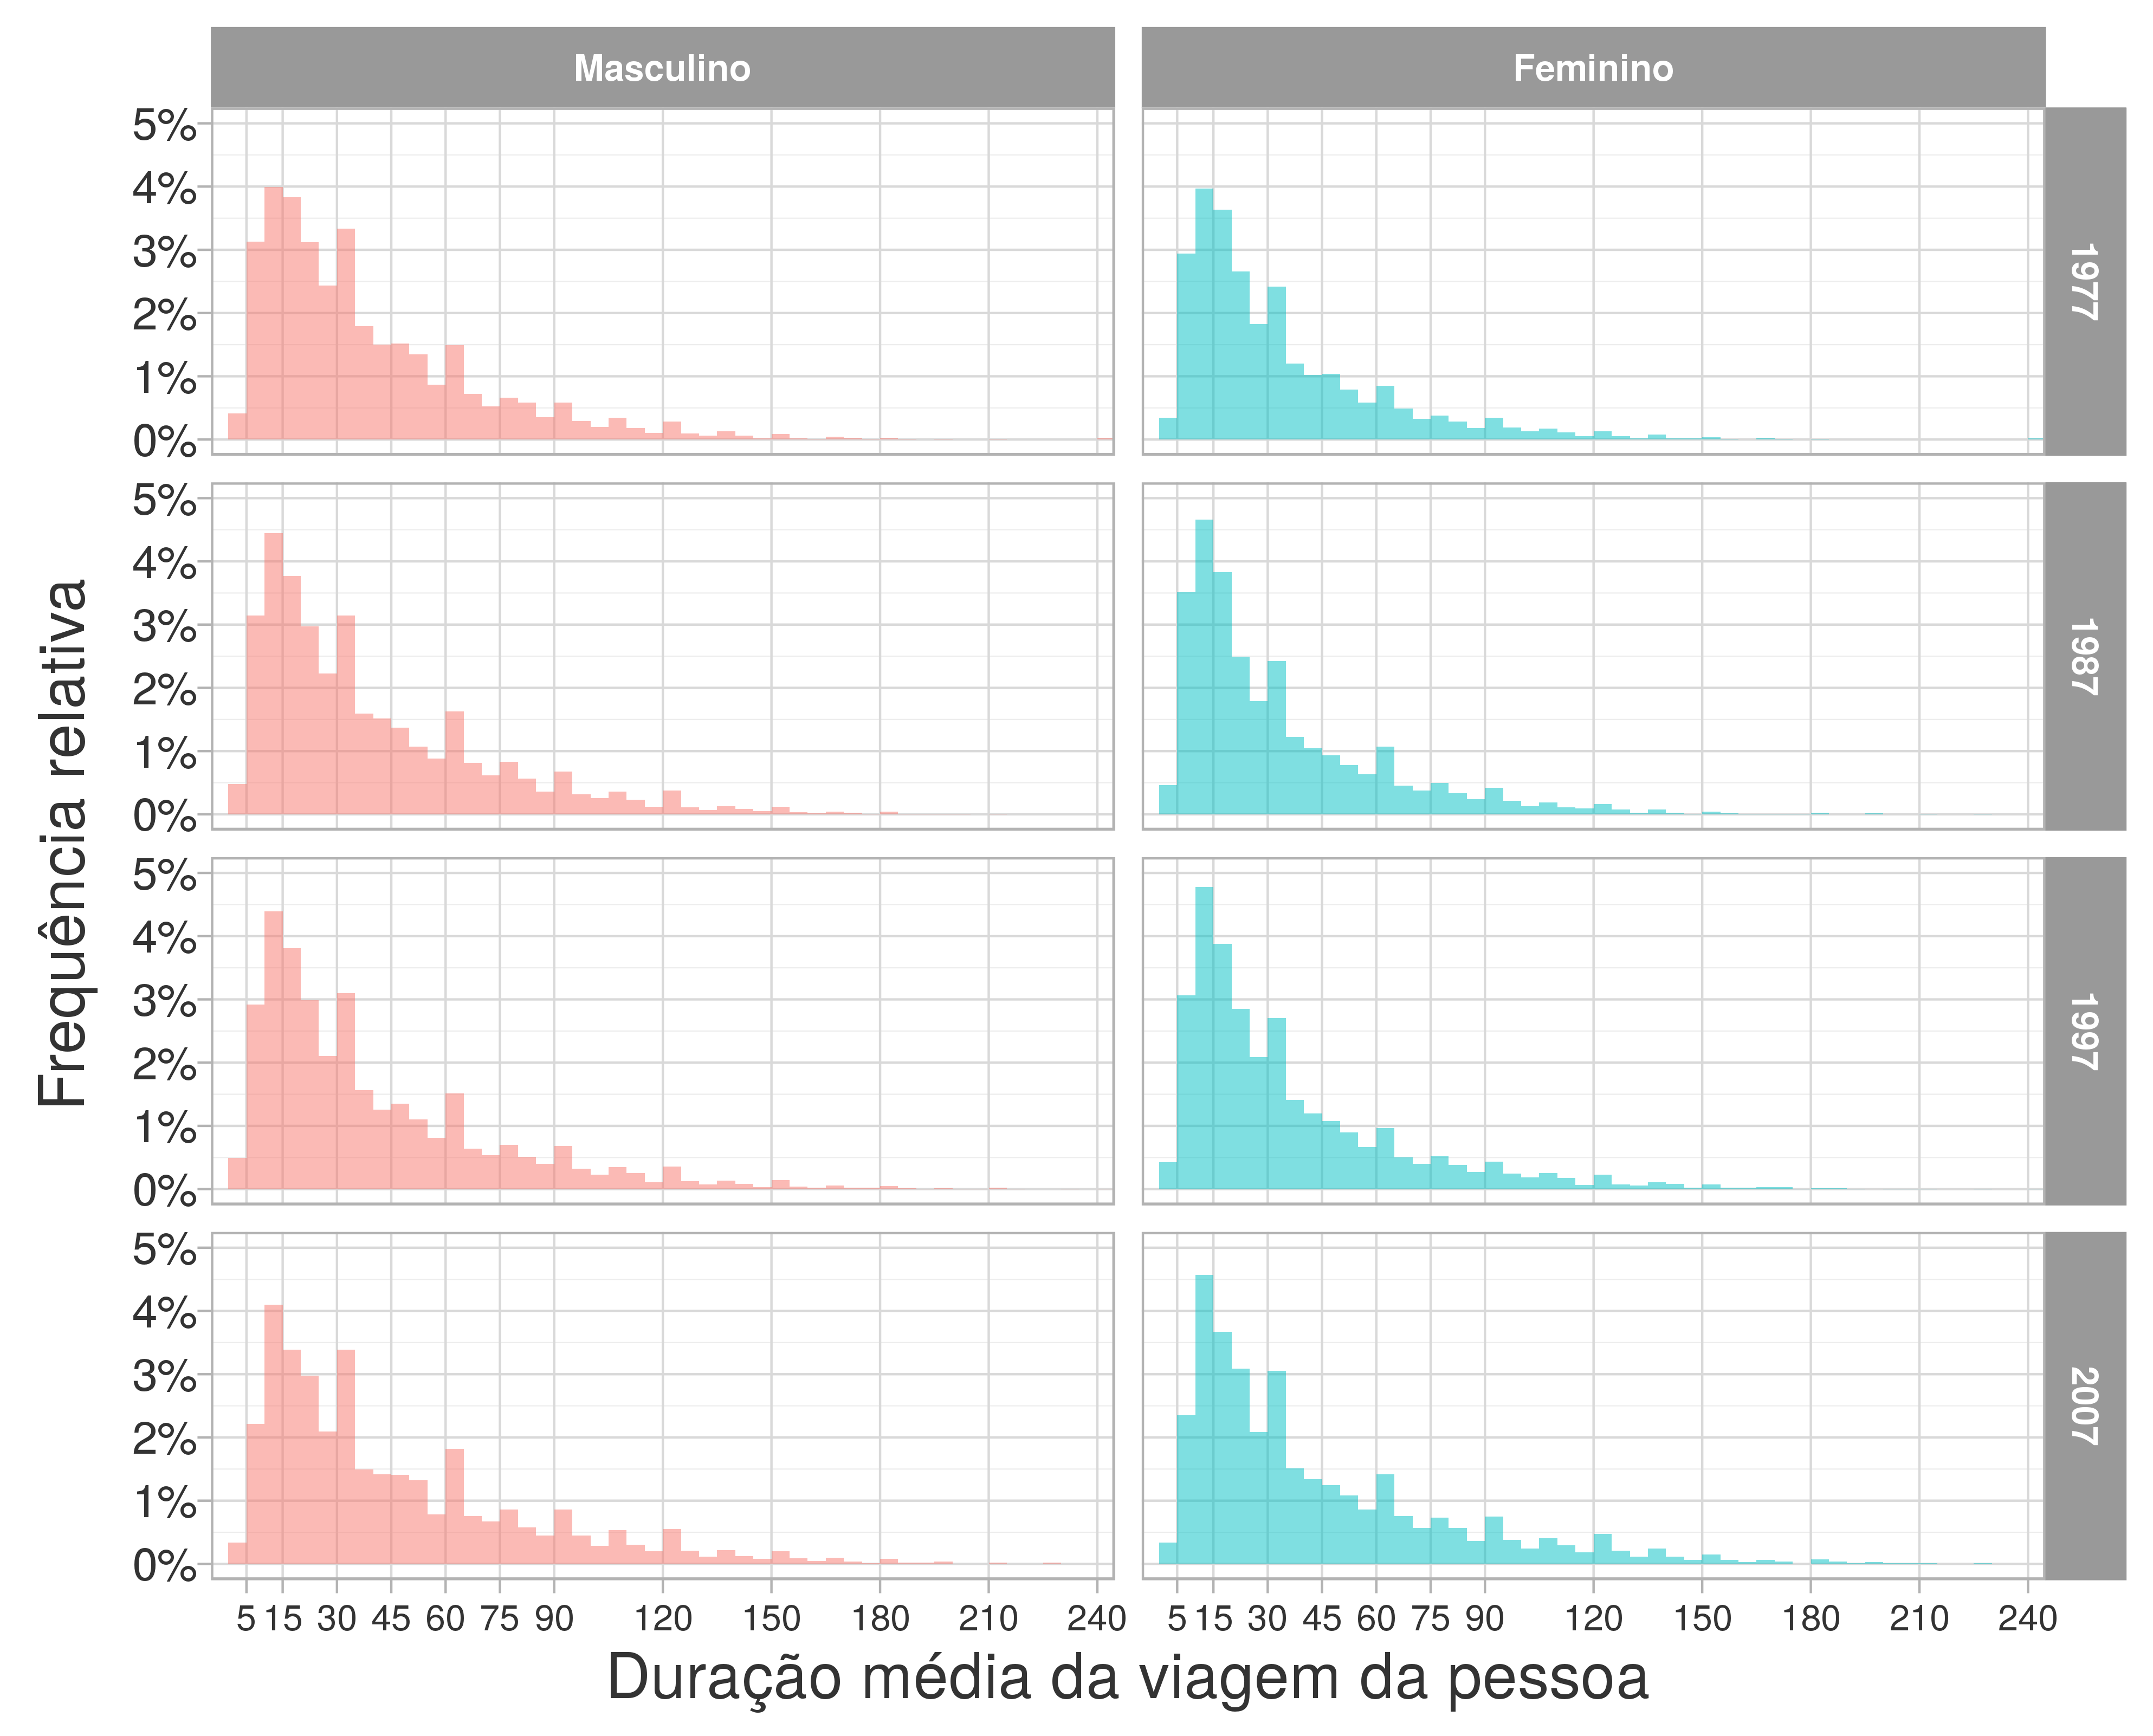
\includegraphics[width=1\textwidth]{./imagens/pess-duracao-med.png}%
%    \end{center}%
%%    \fonte{Compilação própria}
%\end{grafico}%
%% Estatísticas para registros com F_PESS==1 e SEXO
%% Expandido com FE_PESS

%\begin{table}[htb]
%\centering
%   \IBGEtab{%\renewcommand{\arraystretch}{1.5}%%\ABNTEXfontereduzida%
%        \renewcommand{\arraystretch}{1.5}
%        \caption{Estatísticas da variável ``FAM_DURACAO_TOT'', por ano}
%        \label{tab:estat-fam-duracao-tot}
%    }{%
%
%    \begin{tabular}{ccccccc}
%        \toprule
%        \textbf{} & \multicolumn{6}{c}{\textbf{Considerando famílias em que a duração média é superior a 4 minutos}} \\ \hline
%        \textbf{ANO}   & \textbf{Média} & \textbf{Desvio Padrão} & \textbf{Mediana} & \textbf{Máximo} & \textbf{Assimetria} & \textbf{Curtose} \\ \midrule \midrule
%        \textbf{1977}  & 293,14 & 222,68 & 240,00 & 2090 & 1,59 & 3,87 \\ \hline
%        \textbf{1987}  & 265,22 & 199,68 & 220,00 & 2703 & 1,69 & 5,23 \\ \hline
%        \textbf{1997}  & 256,91 & 187,29 & 215,00 & 1890 & 1,42 & 2,87 \\ \hline
%        \textbf{2007}  & 279,18 & 201,34 & 240,00 & 3035 & 1,72 & 9,02 \\\bottomrule          
%
%        \textbf{} & \multicolumn{6}{c}{\textbf{Considerando inclusive família em que ninguém fez viagem}} \\ \hline
%        \textbf{ANO}   & \textbf{Média} & \textbf{Desvio Padrão} & \textbf{Mediana} & \textbf{Máximo} & \textbf{Assimetria} & \textbf{Curtose} \\ \midrule \midrule
%        \textbf{1977}  & 270,74 & 220,08 & 220,00 & 2090 & 1,55 & 3,86 \\ \hline
%        \textbf{1987}  & 251,07 & 200,59 & 210,00 & 2703 & 1,68 & 5,71 \\ \hline
%        \textbf{1997}  & 240,13 & 193,64 & 200,00 & 1890 & 1,37 & 2,87 \\ \hline
%        \textbf{2007}  & 242,07 & 194,09 & 205,00 & 3035 & 1,58 & 7,25 \\\bottomrule
%
%    \end{tabular}
%    }{%
%%		\fonte{Elaboração própria}
%	}
%\end{table}
%% Estatísticas para registros com F_FAM==1, filtro por ANO
%% Expandido com FE_FAM

%O Gráfico \ref{graf:distr-dur-viag} foi construído considerando-se apenas as viagens cuja duração fosse igual ou superior a 5 minutos. Em todos os anos, para homens e para mulheres, percebem-se alguns picos que ocorrem nos valores múltiplos de cinco minutos. Isso porque a duração de viagem é aquela percebida e declarada pelo(a) respondente. Em 1977, a duração das viagens mais curtas (como 5 e 30 minutos) era menos frequente entre as mulheres (13\% e 14\%, respectivamente) do que entre os homens (26\% e 15\%). Em 1987 as viagens de 5 minutos passam a ser mais frequentes entre mulheres (32\%) do que entre homens (26,5\%). Essa situação se inverte em 1997 e retorna em 2007.
%Em todos os anos as viagens mais longas (de 60 e 90 minutos) são mais frequentes entre os homens do que entre as mulheres.
%Na Tabela \ref{tab:dur-med-viag} são apresentadas as durações médias de viagens para homens e mulheres. As médias de homens são superiores às das mulheres, ao nível de significância estatística de 5\%. É possível perceber que a duração média de viagem para ambos vem crescendo e a diferença entre esses grupos vem diminuindo.

A variável \textbf{DURACAO} tem suas principais estatísticas apresentadas na Tabela \ref{tab:estat-duracao}.
Não existem \textit{missing values} neste campo e, desconsiderando quem não fez viagem (duração igual a 0 minutos), o valor mínimo para todos anos e ambos os sexos é 1 minuto.
As medianas da duração, independente do sexo, saem de 30 minutos em 1977 para 20 minutos em 1987 e 1997 e retornam para o valor 30 em 2007.
Os valores de assimetria são todos positivos, indicando maior concentração à esquerda e cauda longa à direita da distribuição.
Os valores de curtose evidenciam não se tratar de distribuição normal.
O tempo médio geral de viagem decresce entre 1977 e 1987 e daí em diante só aumenta, comportamento semelhante ao segmento feminino.
Os tempos médios das viagens do homens cresce sistematicamente década a década, da ordem de 1 minuto entre 1977, 1987 e 1997. Já 2007 o acréscimo no tempo médio de viagem masculino subiu 4,5 minutos - tal efeito pode ser explicado pela expansão urbana da RMSP.
Analisando esses dados segmentados por sexo, vê-se que as medianas das mulheres são sempre 5 minutos a menos que as dos homens. 
A diferença entre as durações médias das viagens de mulheres e de homens cresce de quase 0,5 minuto em 1977 para pouco mais de 5,5 minutos em 1987 e vem diminuindo desde então.
Foram feitos teste t para avaliar se eram estatisticamente significantes (intervalo de confiança de 95\%) as médias entre os sexos, no mesmo ano; e entre os anos, para o mesmo sexo. Todas médias foram estatisticamente diferentes umas das outras.

\begin{table}[htb]
\centering
   \IBGEtab{%\renewcommand{\arraystretch}{1.5}%%\ABNTEXfontereduzida%
        \renewcommand{\arraystretch}{1.5}
        \caption{Estatísticas da variável ``DURACAO'', por ano}
        \label{tab:estat-duracao}
    }{%

    \begin{tabular}{ccccccc}
        \toprule
        \textbf{Total} & \multicolumn{6}{c}{\textbf{}} \\ \hline
        \textbf{ANO}   & \textbf{Média} & \textbf{Desvio Padrão} & \textbf{Mediana} & \textbf{Máximo} & \textbf{Assimetria} & \textbf{Curtose} \\ \midrule \midrule
        \textbf{1977}  & 36,07 & 31,99 & 30 & 240 & 1,74 & 3,78 \\ \hline
        \textbf{1987}  & 33,27 & 31,99 & 20 & 360 & 1,92 & 4,97 \\ \hline
        \textbf{1997}  & 34,13 & 33,52 & 20 & 370 & 1,94 & 4,54 \\ \hline
        \textbf{2007}  & 39,29 & 37,22 & 30 & 299 & 1,74 & 3,37 \\\bottomrule          

        \textbf{Sexo feminino} & \multicolumn{6}{c}{\textbf{}} \\ \hline
        \textbf{ANO}   & \textbf{Média} & \textbf{Desvio Padrão} & \textbf{Mediana} & \textbf{Máximo} & \textbf{Assimetria} & \textbf{Curtose} \\ \midrule \midrule
        \textbf{1977}  & 34,09 & 30,54 & 25 & 240 & 1,81 & 4,12 \\ \hline
        \textbf{1987}  & 30,15 & 29,76 & 20 & 360 & 2,08 & 5,89 \\ \hline
        \textbf{1997}  & 31,97 & 31,67 & 20 & 315 & 2,02 & 4,78 \\ \hline
        \textbf{2007}  & 37,96 & 36,72 & 25 & 299 & 1,81 & 3,68 \\\bottomrule     

        \textbf{Sexo Masculino} & \multicolumn{6}{c}{\textbf{}} \\ \hline
        \textbf{ANO}   & \textbf{Média} & \textbf{Desvio Padrão} & \textbf{Mediana} & \textbf{Máximo} & \textbf{Assimetria} & \textbf{Curtose} \\ \midrule \midrule
        \textbf{1977}  & 34,47 & 32,89 & 30 & 240 & 1,69 & 3,53 \\ \hline
        \textbf{1987}  & 35,83 & 33,50 & 25 & 360 & 1,80 & 4,36 \\ \hline
        \textbf{1997}  & 36,11 & 35,02 & 25 & 370 & 1,86 & 4,25 \\ \hline
        \textbf{2007}  & 40,61 & 37,67 & 30 & 270 & 1,67 & 3,11 \\\bottomrule             

    \end{tabular}
    }{%
%		\fonte{Elaboração própria}
	}
\end{table}
% Estatísticas para registros com F_FAM==1, filtro por ANO
% Expandido com FE_FAM

Com o intuito de melhor explorar as durações médias das viagens analisando modos e motivos, foram elaborados os Gráficos \ref{graf:duracao-modo}, \ref{graf:duracao-coletivo} e \ref{graf:duracao-motivo}.
O Gráfico \ref{graf:duracao-modo} apresenta as durações médias do transporte coletivo, individual e a pé, para homens e para mulheres. Verifica-se que:
\begin{compactitem}[]
\item (i) As durações médias de homens e mulheres são muito próximas para as viagens a pé, girando em torno de 15 minutos para ambos.
\item (ii) A duração média no transporte individual cai um pouco de 1977 para 1987 (de 23,0 para 20,4 min para mulheres e de 27,07 para 25,7 min para homens).
\item (iii) A duração média no transporte individual aumenta de 1987 para 2007 (7,3 min para mulheres e 8,1 min para homens).
\item (iv) A duração média no transporte coletivo aumenta entre 1977 e 2007 para ambos sexos, sendo a taxa mais acentuada de 1997 para 2007. 
\item (v) As diferenças nas durações médias nas viagens feitas por transporte coletivo entre mulheres e homens aumenta de 1977 (4,2 min) para 1987 (6,3 min) e depois decresce nas décadas seguintes (6,0 min em 1997 e 3,2 min em 2007).
\end{compactitem}

\begin{grafico}[htb]%
    \caption{\label{graf:duracao-modo}Durações médias de viagem por ano e por sexo, segundo os modos (agregados)}%
    \begin{center}%
        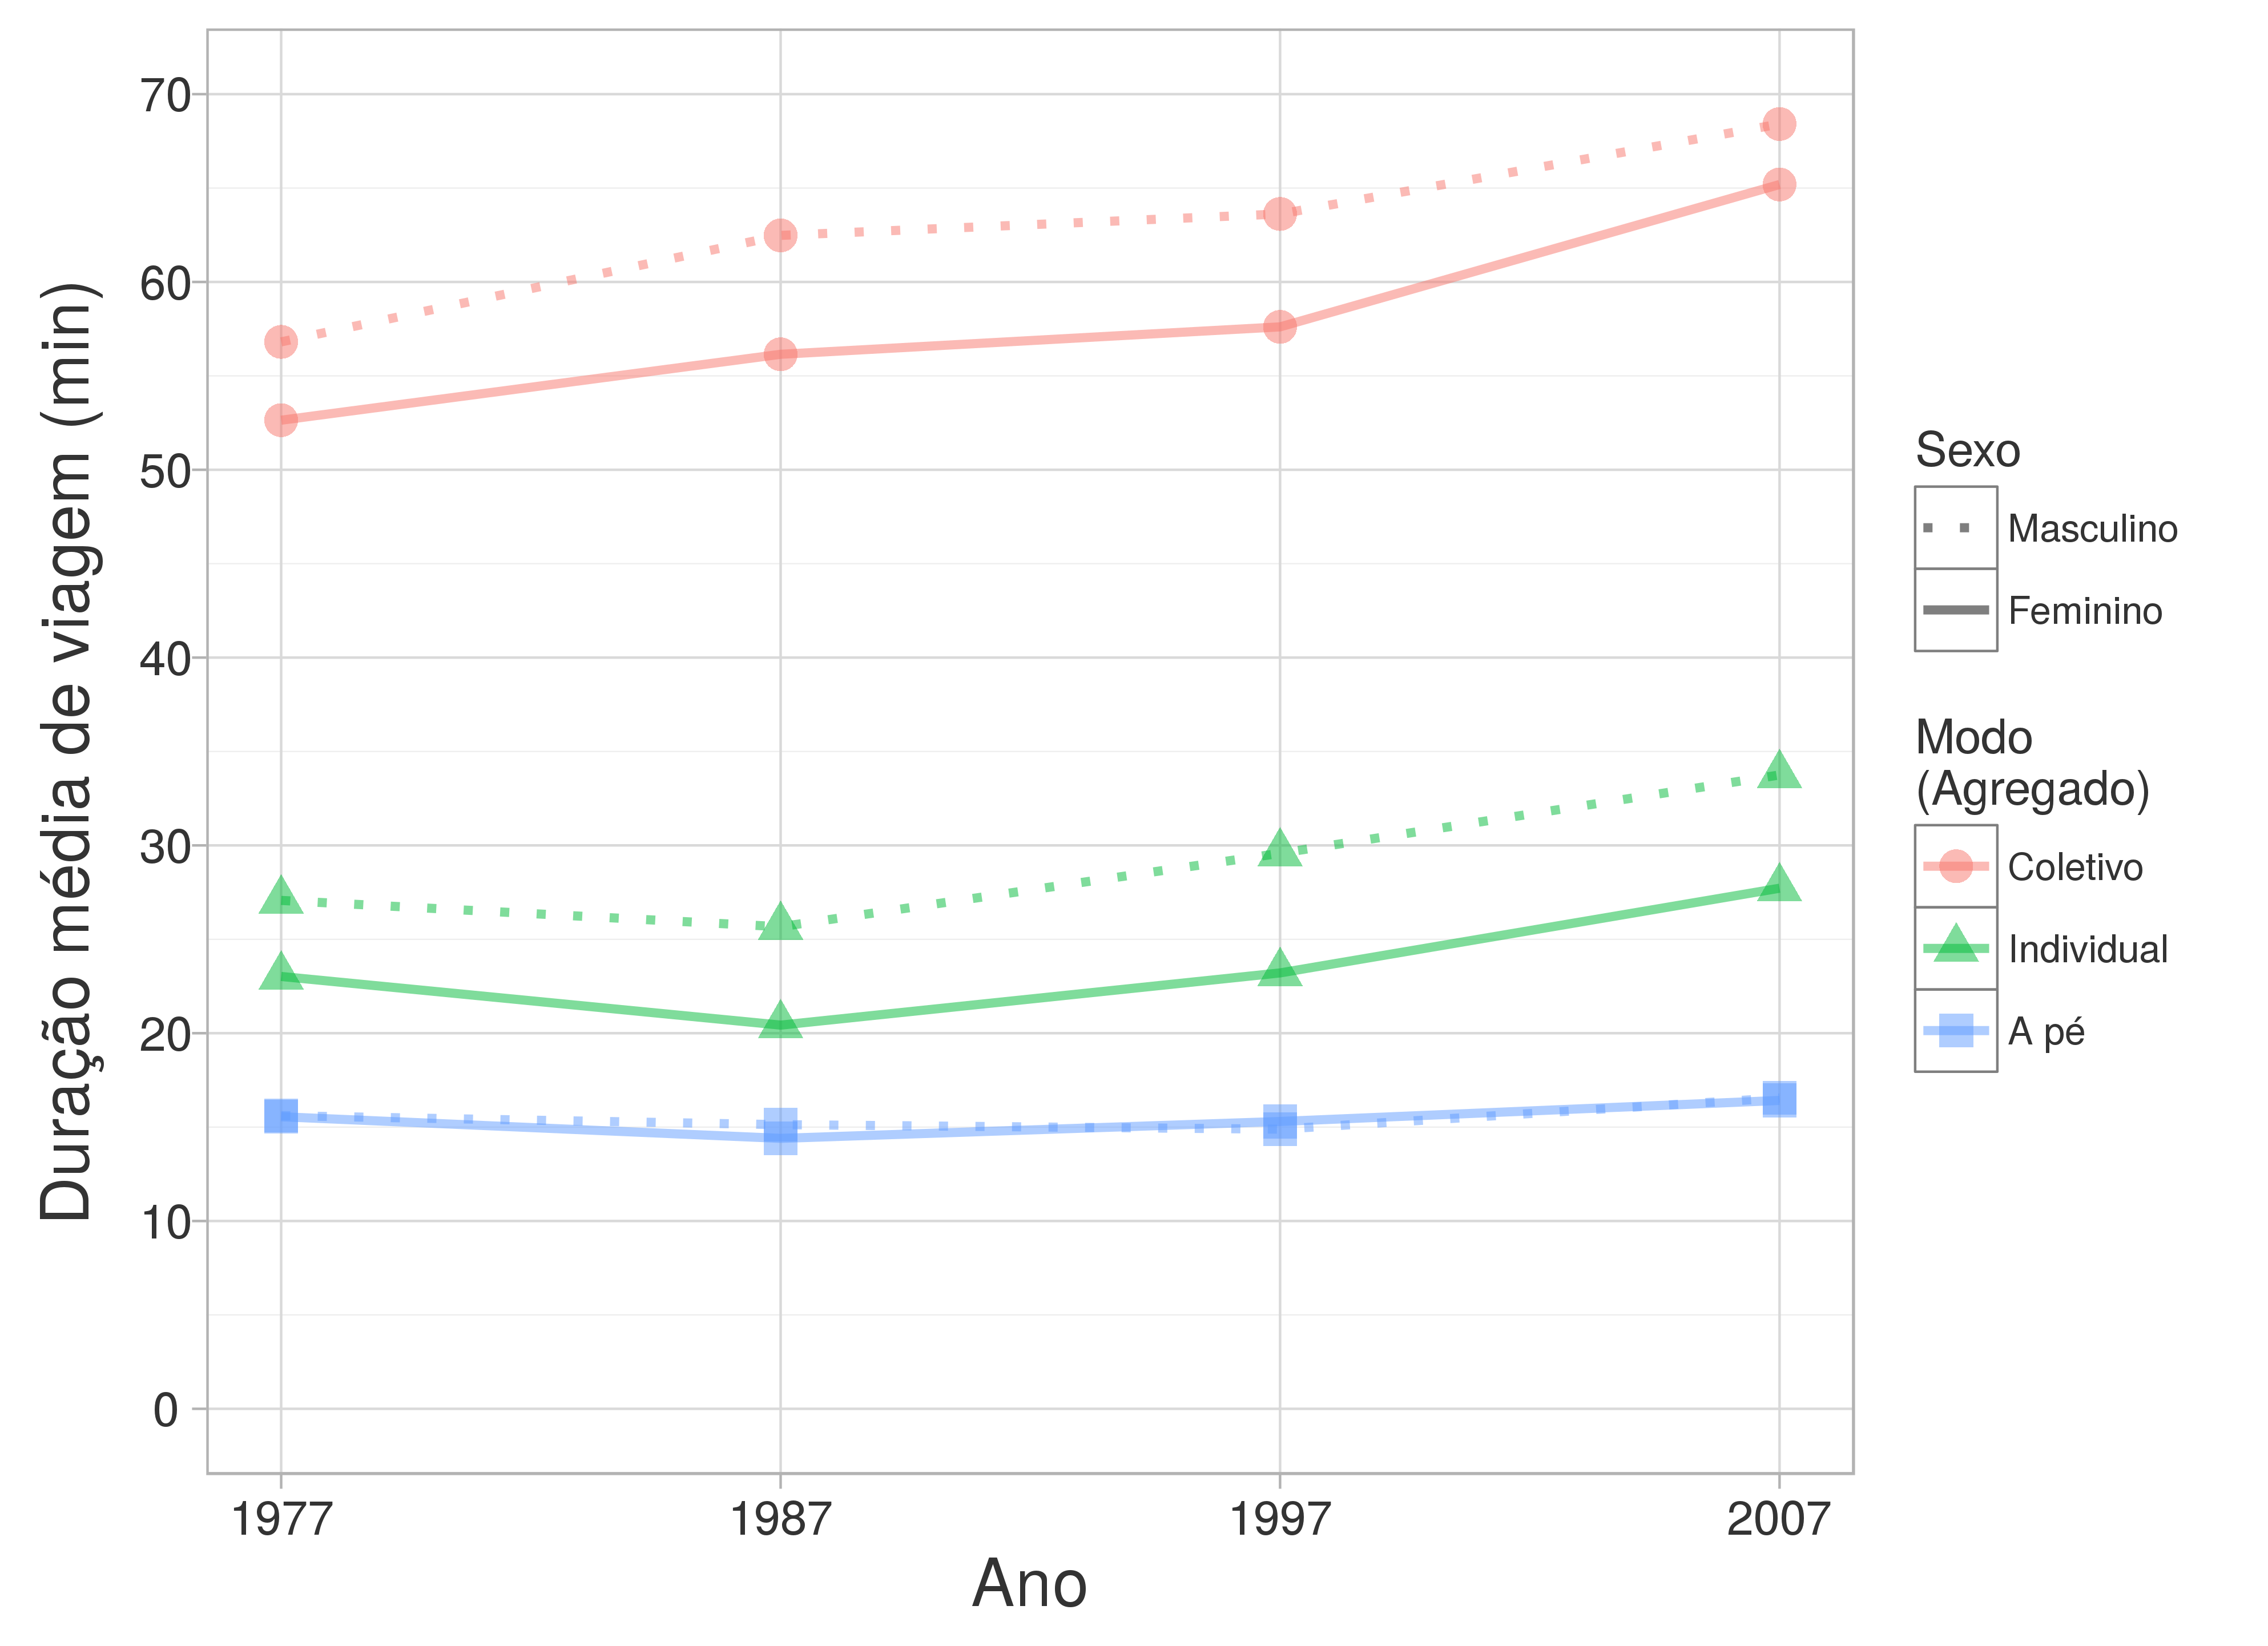
\includegraphics[width=1\textwidth]{./imagens/duracao-modo.png}%
    \end{center}%
%    \fonte{Compilação própria}
\end{grafico}%
% Estatísticas para registros com F_VIAG==1 e SEXO
% Expandido com FE_VIAG

O Gráfico \ref{graf:duracao-coletivo} apresenta as durações médias dos modos de transporte coletivo (ônibus de linha, ônibus de empresa/escolar, lotação/perua/van/microônibus, Metrô e trem), para homens e para mulheres - foram separados os modos de alta capacidade dos demais para facilitar a compreensão dos gráficos. Verifica-se que:
\begin{compactitem}[]
\item (i) A duração média do trem é superior a todos outros modos, inclusive o Metrô, com médias gerais caindo de 83,3 min em 1977 para 80,8 min em 1987 e crescendo para 89,5 min em 1997. Em 2007, esse valor permanece no mesmo patamar de 1997 (91,2 min).
\item (ii) Para o trem, a duração média feminina é inferior à masculina em 1977 (diferença de 2,9 min) e 1987 (diferença de 2,1 min), supera a masculina em 1997 (por 1,5 min) e distancia da masculina em 2007 (diferença de 8,0 min).
\item (iii) A duração média das viagens de Metrô crescem sistematicamente, pelo menos 6 min por década, de 1977 (53,8 min) a 2007 (74,4 min).
\item (iv) Para o Metrô, a duração média feminina é superior à masculina em 1977 (diferença de 1,3 min) e em 2007 (diferença de 1,7 min). A situação é inversa, com durações médias das viagens masculinas superiores às femininas em 1987 (diferença de 3,8 min) e 1997 (diferença de 5,0 min).
\item (v) A duração média das viagens dos ônibus de linha crescem sistematicamente, 5 min entre 1977 e 1987, 0,9 min entre 1987 e 1997, e 8,8 min entre 1997 e 2007.
\item (vi) Para ônibus de linha, a duração média feminina é inferior à masculina - a diferença é de 4,0 min em 1977, de 6,9 min em 1987, de 6,3 min em 1997 e de 3,9 min em 2007.
\item (vii) A duração média das viagens de lotações/vans crescem de 1977 (54,1 min) para 1987 (60,8 min), caem em 1997 (49,9 min) e sobem novamente em 2007 (66,3 min).
\item (viii) Para viagens de lotações/vans, a duração média feminina era inferior à masculina em 1977 (diferença de 6,4 min) e em 2007 (diferença 9,4 de min). A situação é inversa em 1987, com diferenças de 7,7 min entre os sexos. E, em 1997, as durações médias são estatisticamente iguais.
\item (ix) A duração média das viagens de ônibus escolar/fretado são as menores entre os transportes coletivos, para ambos sexos variando numa faixa de 40,9 a 44,2 min.
\item (x) Para viagens de ônibus escolar/fretado, a duração média feminina é sempre inferior à masculina - a diferença é de 6,8 min em 1977, de 7,2 min em 1987, de 7,1 min em 1997 e de 2,9 min em 2007.
\end{compactitem}

\begin{grafico}[htb]%
    \caption{\label{graf:duracao-coletivo}Durações médias de viagem por ano e por sexo, segundo os modos coletivos}%
    \begin{center}%
        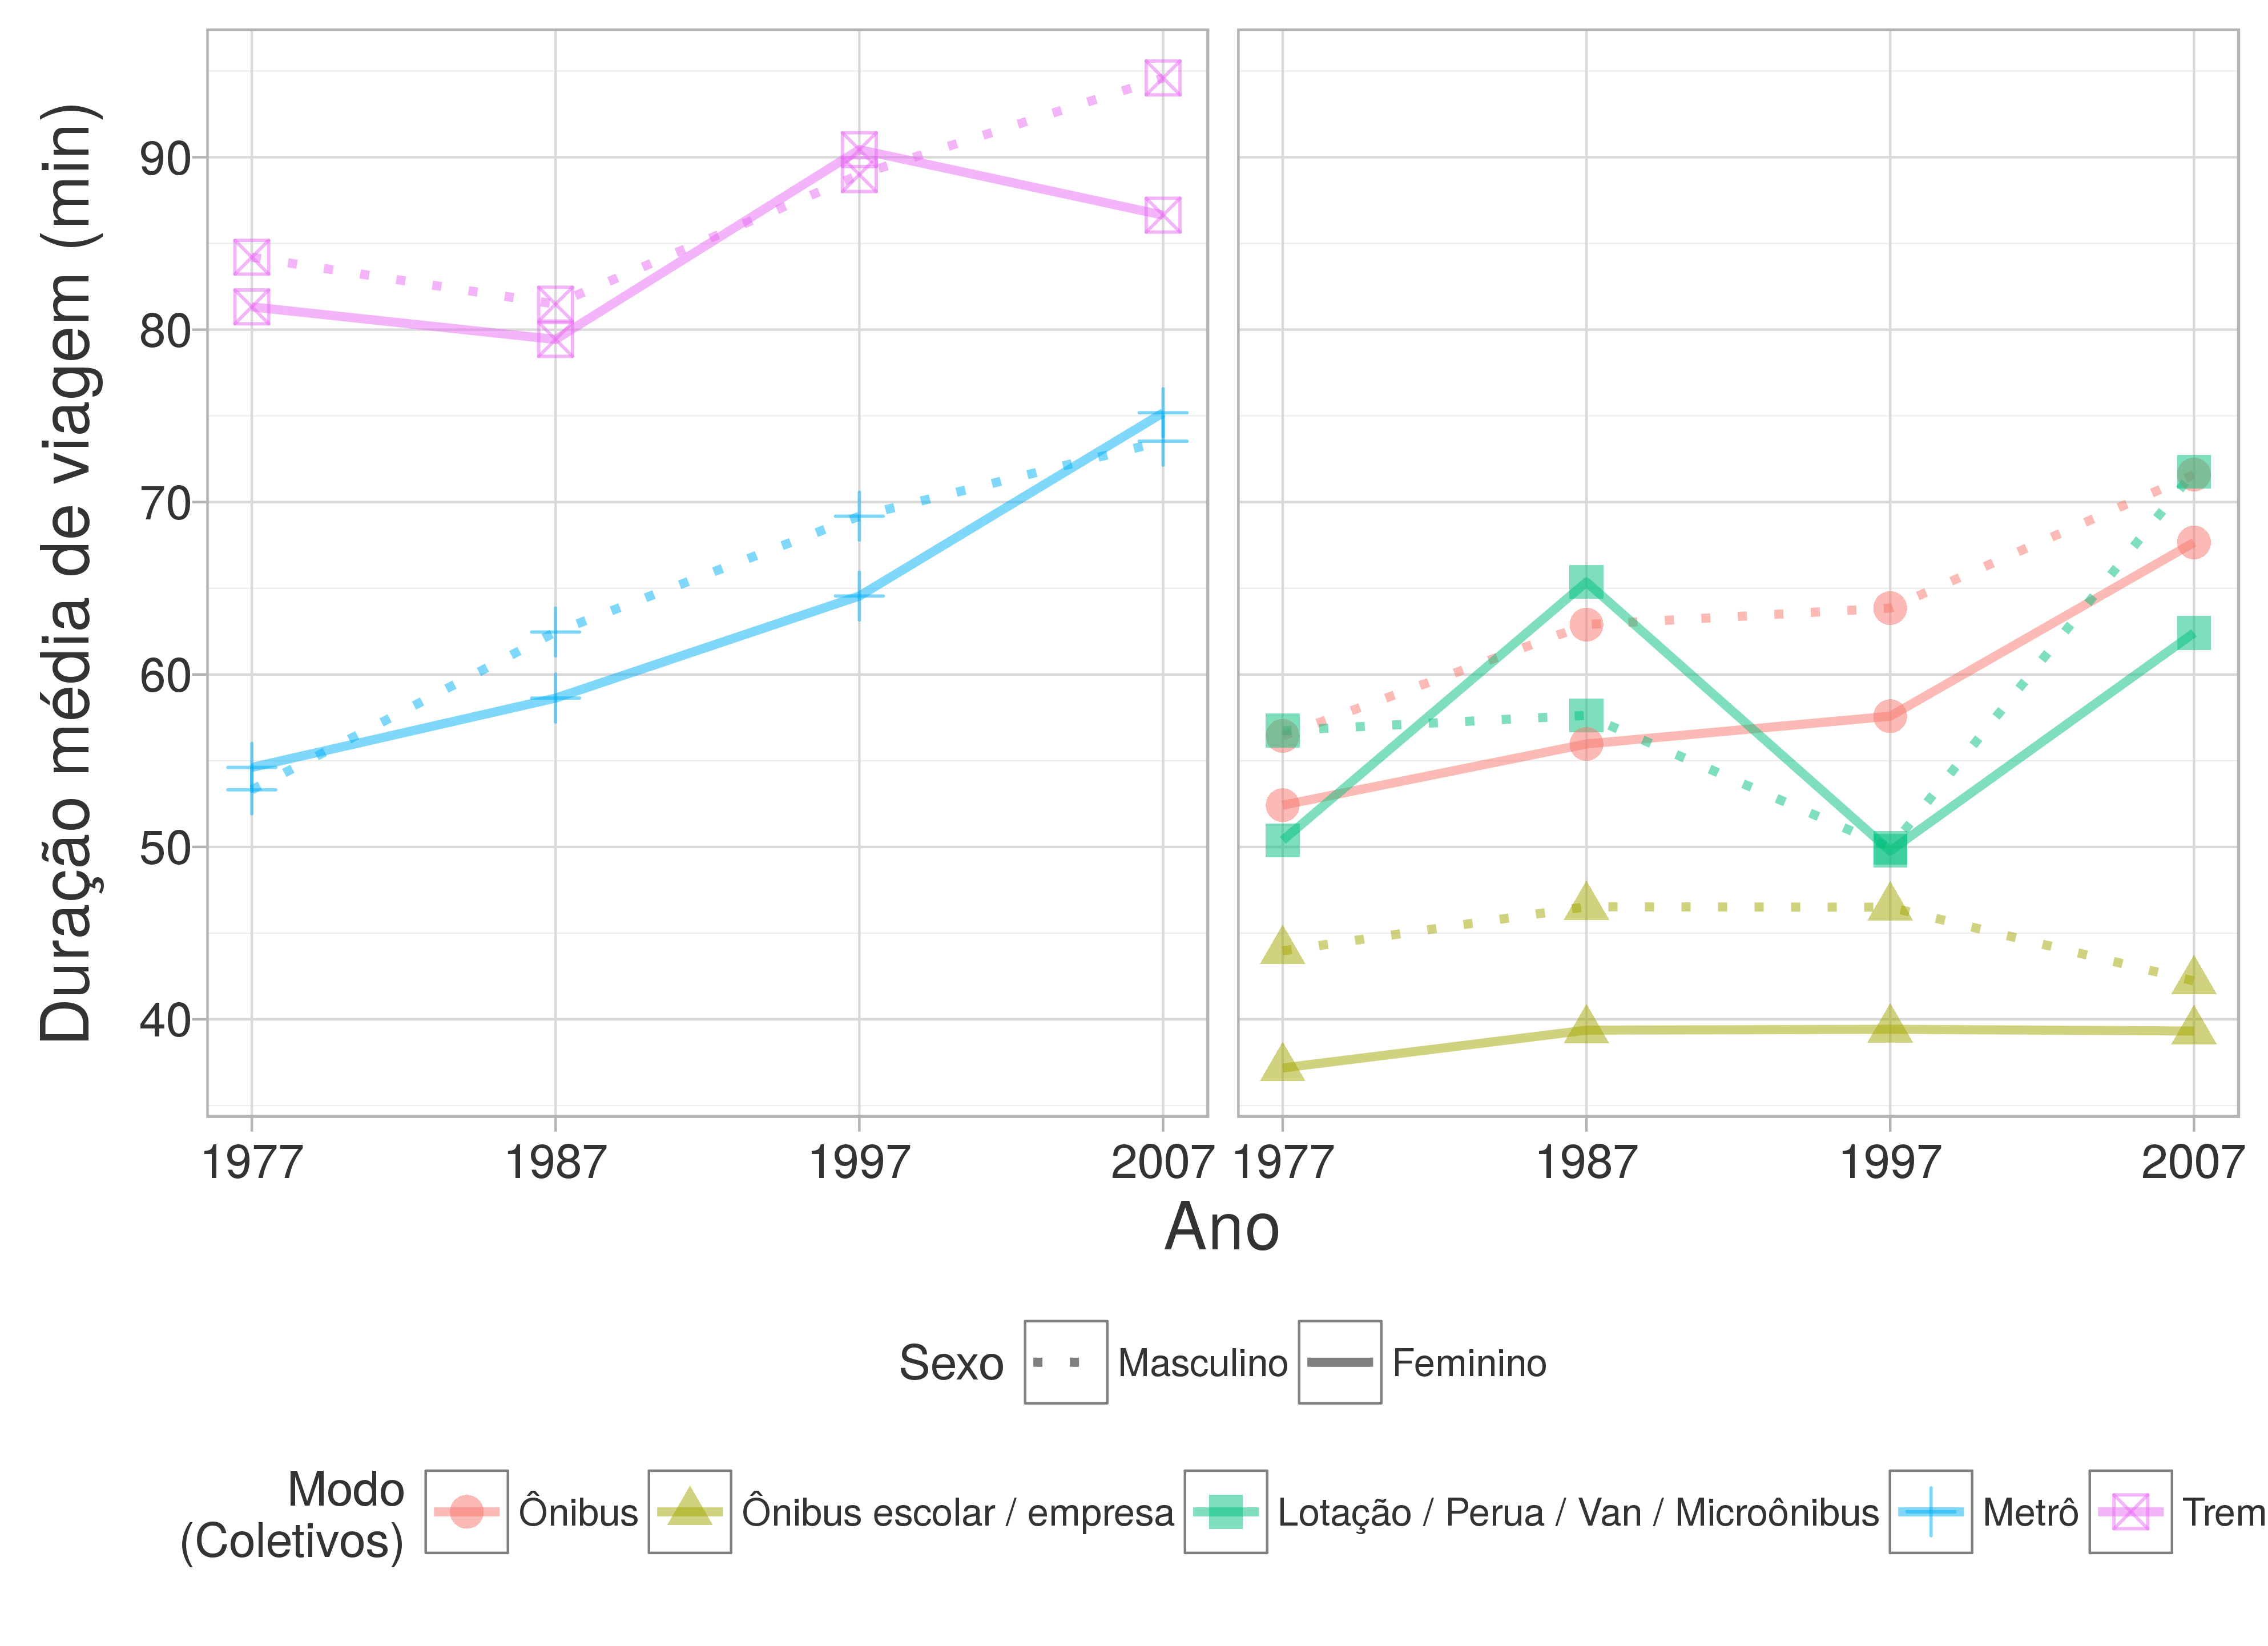
\includegraphics[width=1\textwidth]{./imagens/duracao-coletivo.png}%
    \end{center}%
%    \fonte{Compilação própria}
\end{grafico}%
% Estatísticas para registros com F_VIAG==1 e SEXO
% Expandido com FE_VIAG

O Gráfico \ref{graf:duracao-motivo} apresenta as durações médias por motivo de viagem (trabalho, educação, servir passageiro, manutenção/compras e lazer/outros), para homens e para mulheres. Verifica-se que:
\begin{compactitem}[]
\item (i) A duração média da viagem motivo trabalho (de natureza compulsória) é superior a de todos outros motivos. Ela permanece no mesmo patamar entre 1977 (40,9 min) e 1987 (40,8 min), sobe um pouco em 1997 (42,7 min) e continua a subir em 2007 (48,9 min).
\item (ii) Para o motivo trabalho, a duração média feminina é estatisticamente igual à masculina em 1977, inferior, em 1987 (diferença de 2,5 min) e em 1997 (diferenças de 1,3 min) e levemente superior em 2007 (0,7 min).
\item (iii) A duração média das viagens motivo educação decresce de 1977 (20,9 min) para 1987 (18,3 min), a partir de quando sobem até 2007 (26,1 min).
\item (iv) Para o motivo educação, a duração média feminina é praticamente igual à masculina em 1977 e em 1997 (diferenças de menos de 0,4 min), levemente inferior à masculina em 1987 (diferença de 0,9 min) e superior em 2007 (diferença de 0,6 min).
\item (v) A duração média das viagens motivo manutenção/compras decresce de 1977 (35,2 min) para 1987 (33,9 min), a partir de quando sobem até 2007 (38,0 min).
\item (vi) Para viagens motivo manutenção/compras, a duração média feminina é inferior à masculina - a diferença é de 1,9 min em 1977, de 0,7 min em 1987, de 3,3 min em 1997 e de 0,7 min em 2007.
\item (vii) A duração média das viagens motivo lazer/outros decresce de 1977 (34,3 min) para 1987 (32,9 min), a partir de quando sobem até 2007 (35,6 min).
\item (viii) Para o motivo lazer/outros, a duração média feminina é praticamente igual à masculina em 1997, sendo antes disso inferior à masculina (diferenças de 0,6 e 2,4 min para 1977 e 1987, respectivamente) e depois disso superior à masculina (diferença de 0,9 min em 2007).
\item (ix) A duração média das viagens motivo servir passageiro decresce de 1977 (37,2 min) para 1997 (20,4 min), a partir de quando sobem até 2007 (23,1 min). Vale destacar que em 1987 não havia o modo servir passageiro.
\item (x) Para viagens motivo servir passageiro,  a duração média feminina é estatisticamente igual à masculina em 1977, e inferior em 1997 (diferenças de 1,6 min) e em 2007 (diferenças de 2,7 min).
\end{compactitem}


\begin{grafico}[htb]%
    \caption{\label{graf:duracao-motivo}Durações médias de viagem por ano e por sexo, segundo o motivo da viagem}%
    \begin{center}%
        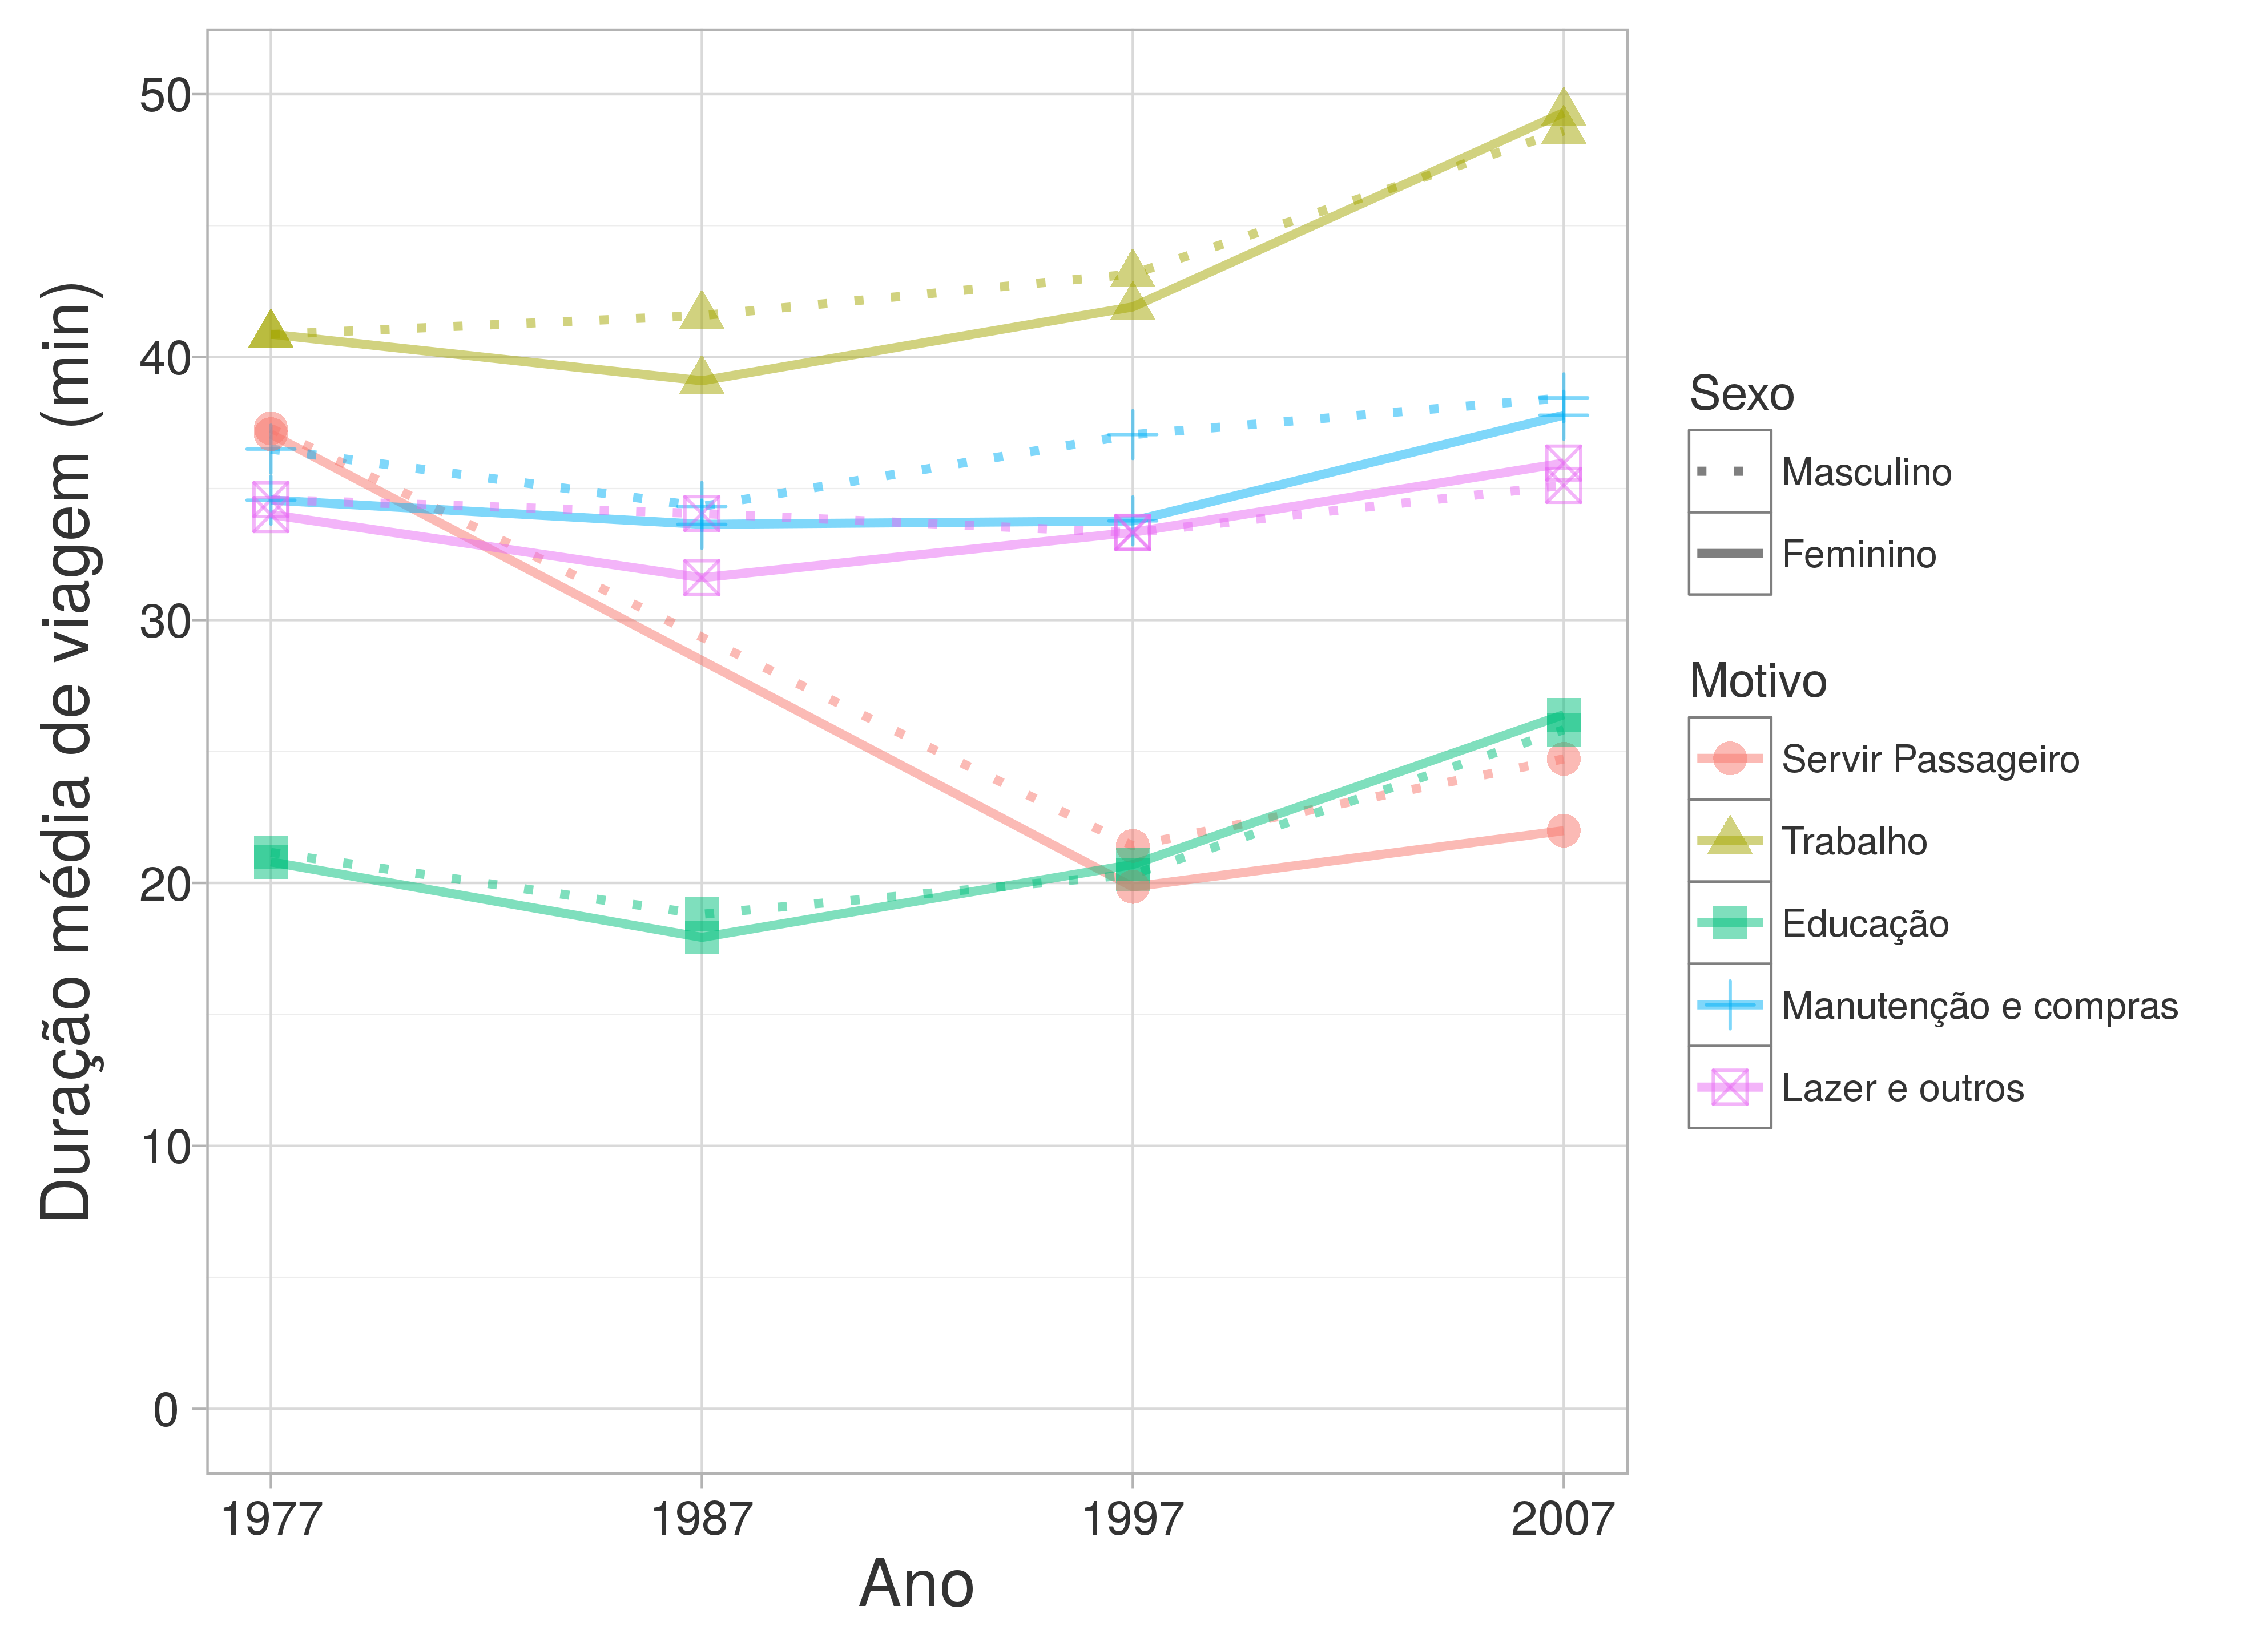
\includegraphics[width=1\textwidth]{./imagens/duracao-motivo.png}%
    \end{center}%
%    \fonte{Compilação própria}
\end{grafico}%
% Estatísticas para registros com F_VIAG==1 e SEXO
% Expandido com FE_VIAG

%TODO ?? Fazer DURACAO (médias) por faixas etárias / situação familliar
%Tendo em vista ainda as questões apontadas na revisão de literatura a respeito da mobilidade/imobilidade das pessoas e formas de mensurá-la, pretende-se avaliar a distância média das viagens em função das variáveis sexo, idade, renda familiar, renda individual, estado civil e presença de filhos da família \cite{ROSENBLOOM2006,SHEARMUR2006,HANSON2010}.

Em ``Estatísticas sob Suspeita'', \citeauthoronline{CARRASCO2012} (\citeyear{CARRASCO2012}, p.100-101) propõe indicadores com base na experiência das mulheres e, especificamente, no capítulo relativo ao acesso à mobilidade e ao planejamento territorial, recomenda a formulação e consideração dos seguintes indicadores quando da formulação de políticas públicas:
motivos dos deslocamentos, meio utilizado nos deslocamentos e distâncias dos deslocamentos, entre outros.
Anteriormente foram apresentados os panoramas de motivos e modos, agora, serão exploradas as distâncias de deslocamento.

A variável de distância da viagem (\textbf{DIST_VIAG}) contém a distância euclidiana entre as coordenadas de origem e as coordenadas de destino, com as limitações que a determinação dessas coordenadas impõem, já que foram calculadas a partir dos centroides das subzonas ou zonas (na ausência das subzonas). Ou seja, para 1977, as distâncias representadas são apenas as inter-zonais, pois não haviam dados disponíveis nem de subzonas nem de coordenadas. Para 1987 e 1997, cujos mapas de subzonas foram disponibilizados, as distâncias representadas são as inter-subzonas. Ainda para 1997, diversas distâncias de viagens não foram possíveis de ser calculadas porque o \textit{shapefile} obtido junto ao Metrô-SP não continha todas subzonas indicadas no banco de dados da Pesquisa OD correspondente. E para 2007, mediante a disponibilidade de melhores recursos tecnológicos, as distâncias apresentadas são mais precisas e obtidas diretamente das coordenadas. Assim, os valores, análises e eventuais resultados decorrentes das distâncias de viagem precisam ser olhados com parcimônia. As principais estatísticas desta variável, cuja unidade é quilômetros, são apresentadas na Tabela \ref{tab:estat-distancia}.

Não existem \textit{missing values} neste campo e, considerando apenas viagens com distância superior a zero, independentemente do sexo, os valores mínimos são: 0,37 km para 1977, 0,35 km para 1987, 0,23 km para 1997 e 0,01 para 2007.
As medianas da distância de viagem, também independente do sexo, crescem ao longo do período analisado, saindo de 5,62 km em 1977 para 5,79 km em 2007.
Os valores de assimetria são todos positivos, indicando maior concentração à esquerda e cauda longa à direita da distribuição.
Os valores de curtose evidenciam não se tratar de distribuição normal.
A distância média geral de viagem sempre aumenta no período analisado: 0,5 km de 1977 para 1987, 0,13 km de 1987 para 1997 e 0,44 km de 1997 para 2007.

Analisando esses dados segmentados por sexo, observa-se que as distâncias médias das viagens do homens cresce década a década e é sempre superior às das mulheres.
As distâncias médias das viagens das mulheres também cresce no período saindo de 6,64 km em 1977 e chegando a 7,80 km em 2007, valor inferior média masculina em 1977.
As diferenças entre os valores médios de mulheres e homens gira em torno de 1,5 km: 1,2 km para 1977, 1,6 km para 1987, 1,7 km para 1997 e 1,3 km para 2007.
Foram feitos teste t para avaliar se as médias entre os sexos, para o mesmo ano, e entre os anos, para o mesmo sexo, eram diferentes. Com um intervalo de confiança de 95\%, todos o p-valores obtidos indicavam ser possível rejeitar a hipótese nula de que a diferença entre as médias eram iguais a zero.

\begin{table}[htb]
\centering
   \IBGEtab{%\renewcommand{\arraystretch}{1.5}%%\ABNTEXfontereduzida%
        \renewcommand{\arraystretch}{1.5}
        \caption{Estatísticas da variável ``DIST_VIAG'', por ano}
        \label{tab:estat-distancia}
    }{%

    \begin{tabular}{ccccccc}
        \toprule
        \textbf{Total} & \multicolumn{6}{c}{\textbf{}} \\ \hline
        \textbf{ANO}   & \textbf{Média} & \textbf{Desvio Padrão} & \textbf{Mediana} & \textbf{Máximo} & \textbf{Assimetria} & \textbf{Curtose} \\ \midrule \midrule
        \textbf{1977}  & 7,40 & 6,06 & 5,62 &  70,38 & 1,91 & 5,71 \\ \hline
        \textbf{1987}  & 7,90 & 6,92 & 5,67 & 107,33 & 1,90 & 5,31 \\ \hline
        \textbf{1997}  & 8,03 & 7,64 & 5,69 &  82,27 & 1,86 & 4,85 \\ \hline
        \textbf{2007}  & 8,47 & 8,15 & 5,79 &  84,10 & 1,73 & 4,05 \\ \bottomrule          

        \textbf{Sexo feminino} & \multicolumn{6}{c}{\textbf{}} \\ \hline
        \textbf{ANO}   & \textbf{Média} & \textbf{Desvio Padrão} & \textbf{Mediana} & \textbf{Máximo} & \textbf{Assimetria} & \textbf{Curtose} \\ \midrule \midrule
        \textbf{1977}  & 6,64 & 5,47 & 5,04 &  65,91 & 2,00 & 6,62 \\ \hline
        \textbf{1987}  & 6,92 & 6,26 & 4,82 & 107,33 & 2,09 & 6,75 \\ \hline
        \textbf{1997}  & 7,09 & 6,89 & 4,90 &  82,27 & 1,95 & 5,27 \\ \hline
        \textbf{2007}  & 7,80 & 7,73 & 5,16 &  82,67 & 1,80 & 4,42 \\ \bottomrule     

        \textbf{Sexo Masculino} & \multicolumn{6}{c}{\textbf{}} \\ \hline
        \textbf{ANO}   & \textbf{Média} & \textbf{Desvio Padrão} & \textbf{Mediana} & \textbf{Máximo} & \textbf{Assimetria} & \textbf{Curtose} \\ \midrule \midrule
        \textbf{1977}  & 7,89 & 6,37 & 6,08 & 70,38 & 1,83 & 5,15 \\ \hline
        \textbf{1987}  & 8,57 & 7,26 & 6,31 & 81,19 & 1,78 & 4,59 \\ \hline
        \textbf{1997}  & 8,82 & 8,13 & 6,36 & 81,05 & 1,76 & 4,34 \\ \hline
        \textbf{2007}  & 9,08 & 8,48 & 6,44 & 84,10 & 1,66 & 3,71 \\ \bottomrule             

    \end{tabular}
    }{%
%		\fonte{Elaboração própria}
	}
\end{table}
% Estatísticas para registros com F_FAM==1, filtro por ANO
% Expandido com FE_FAM

Com o intuito de melhor explorar as distâncias médias das viagens analisando modos e motivos, foram elaborados os Gráficos \ref{graf:distancia-modo}, \ref{graf:distancia-coletivo} e \ref{graf:distancia-motivo}.
O Gráfico \ref{graf:distancia-modo} apresenta as distâncias médias de viagem do transporte coletivo, individual e a pé, para homens e para mulheres. Verifica-se que:
\begin{compactitem}[]
\item (i) As distâncias médias de homens e mulheres são muito próximas para as viagens a pé ($\sim$ 75 m), sequer sendo estatisticamente significativa a diferença em 1997.
\item (ii) A distância média no transporte individual sobe em taxas crescentes a cada década (0,2 km de 1977 para 1987, 0,3 km de 1987 para 1997, e 0,5 km de 1997 para 2007).
\item (iii)  As diferenças nas distâncias médias de viagem feitas por transporte individual entre mulheres e homens aumenta de 1977 (1,7 km) para 1987 (1,9 km) e para 1997 (2,2 km), depois decresce em 2007 (2,1 km).
\item (iv) A distância média no transporte coletivo aumenta entre 1977 e 2007 para ambos sexos, sendo que o ritmo de crescimento vem diminuindo: diferença de 1,1 km entre 1977 e 1987, diferença de 0,5 km entre 1987 e 1997 e diferença de 0,4 km entre 1997 e 2007.
\item (v)  As diferenças nas distâncias médias de viagem feitas por transporte coletivo entre mulheres e homens aumenta de 1977 (1,3 km) para 1987 (1,7 km) e para 1997 (2,0 km), depois decresce em 2007 (1,4 km).
\end{compactitem}

\begin{grafico}[htb]%
    \caption{\label{graf:distancia-modo}Distâncias médias de viagem por ano e por sexo, segundo os modos (agregados)}%
    \begin{center}%
        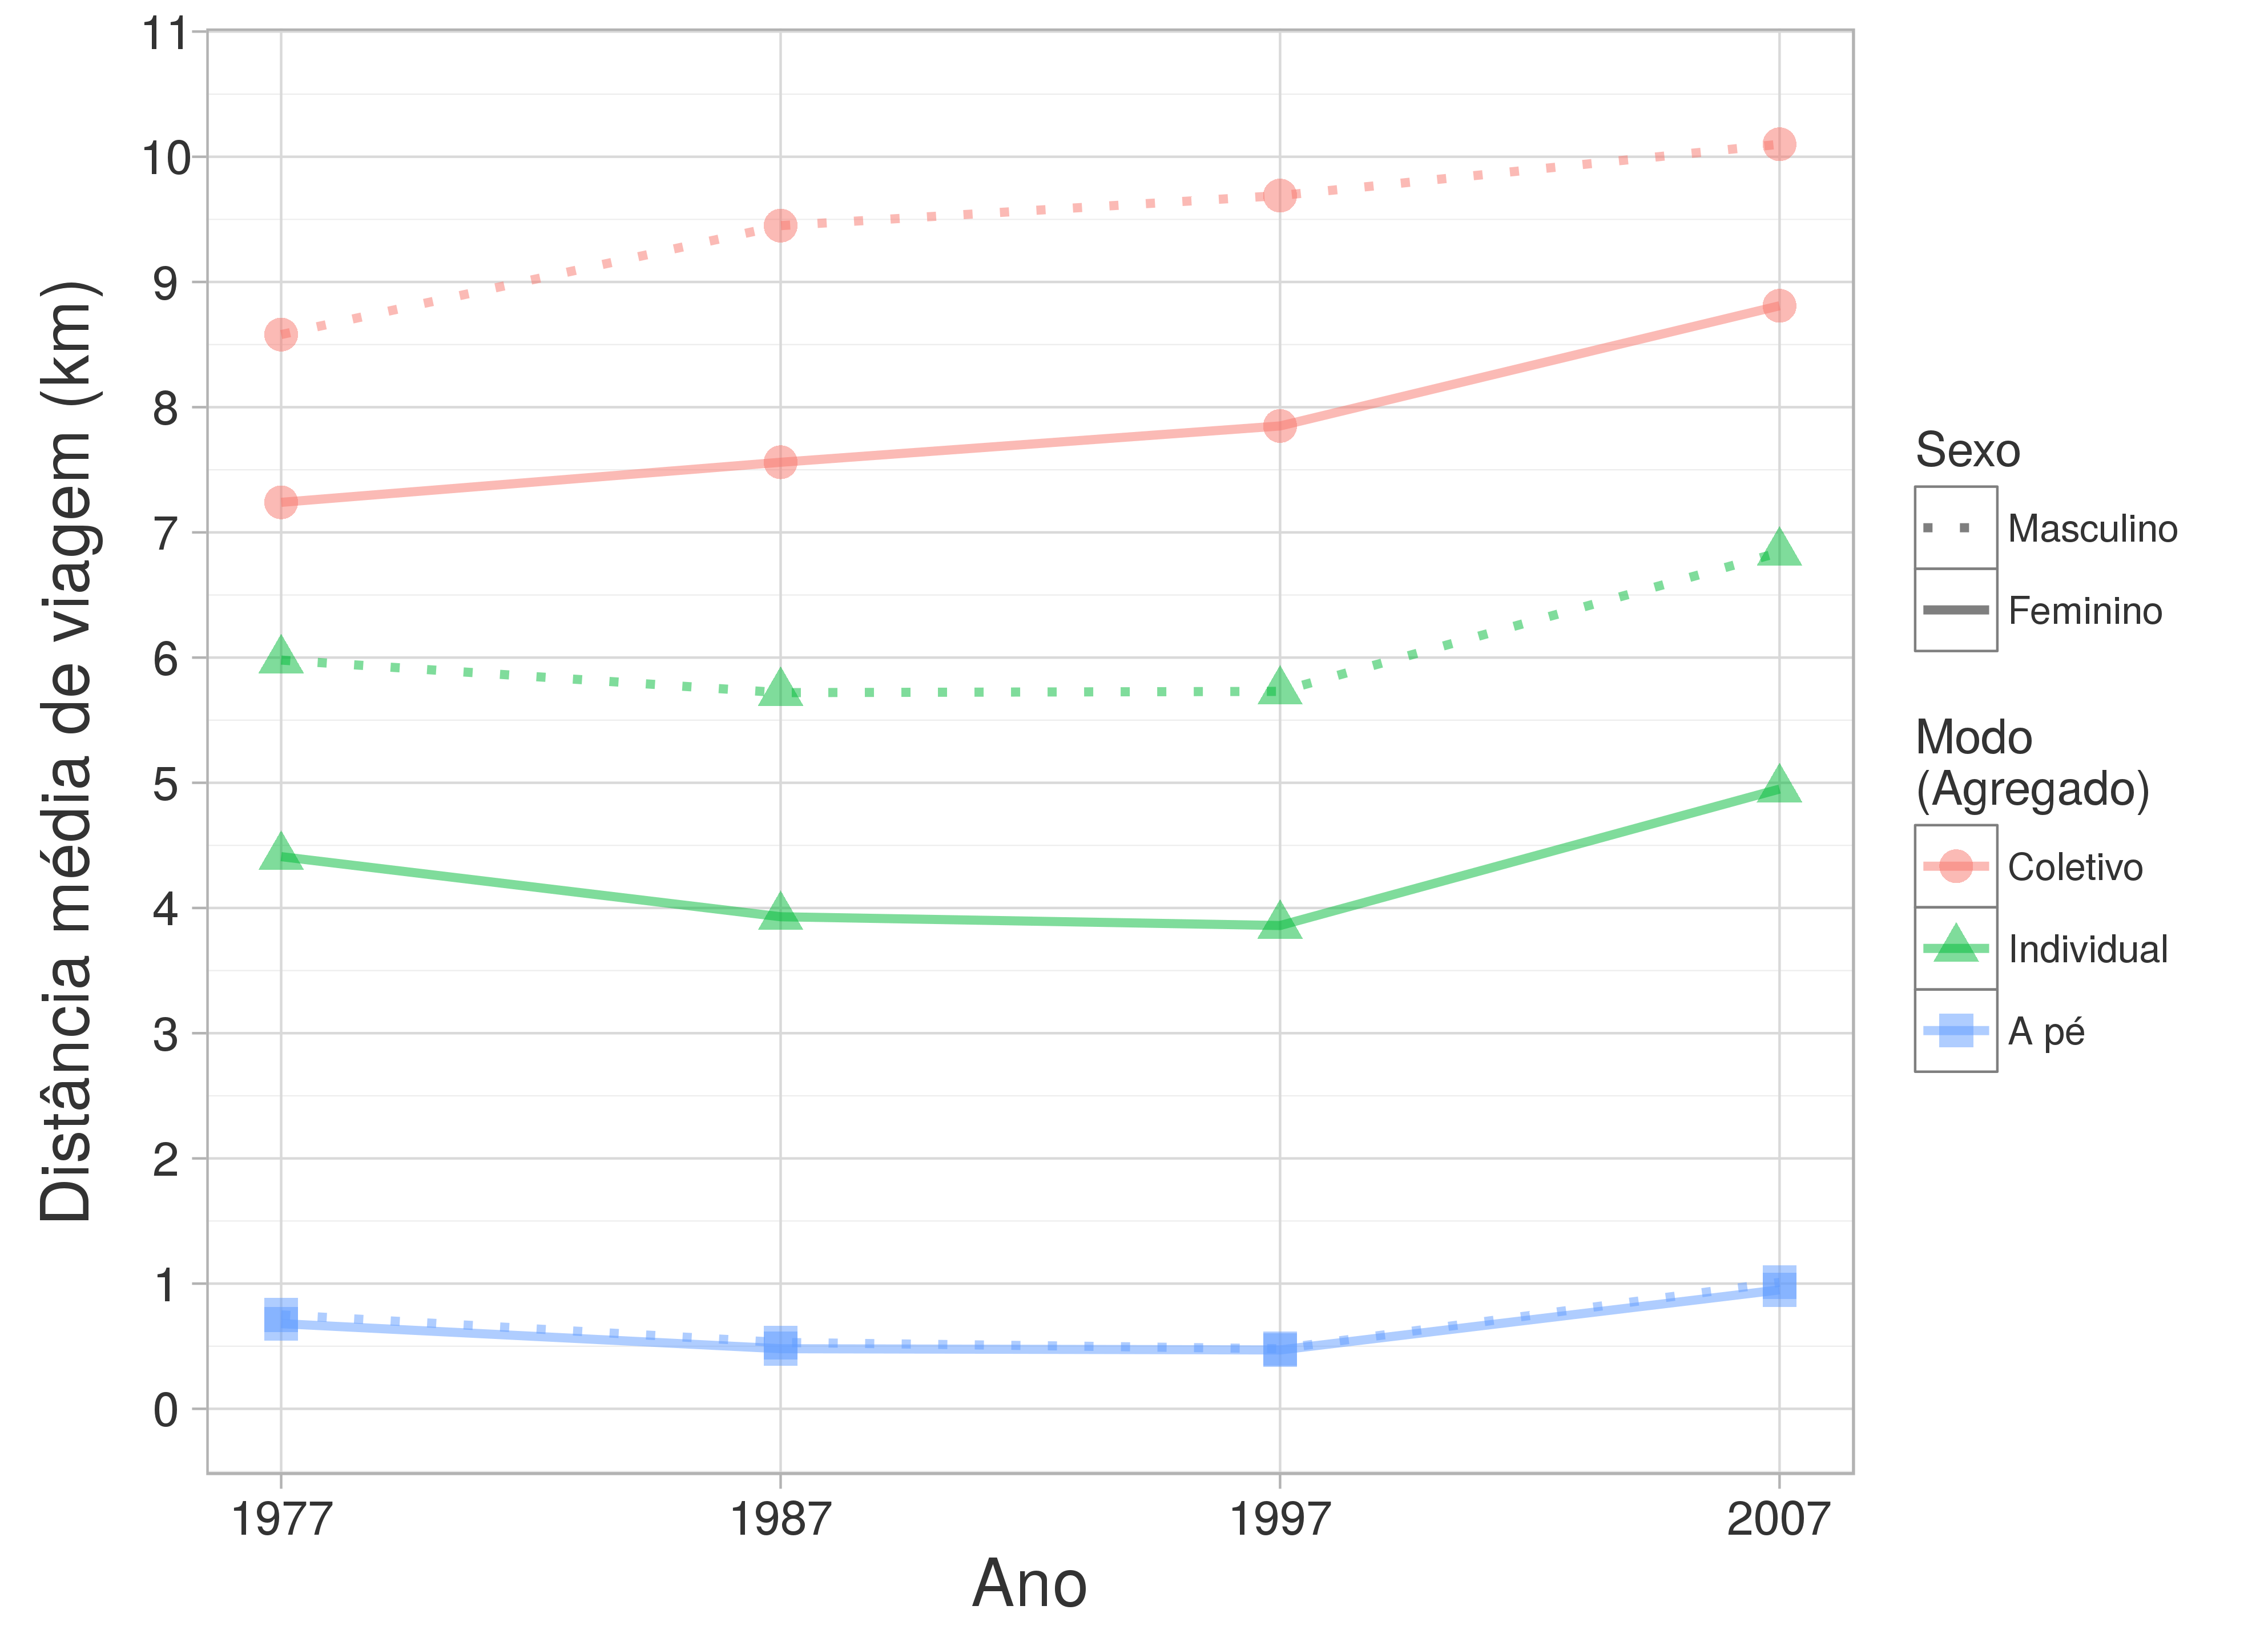
\includegraphics[width=1\textwidth]{./imagens/distancia-modo.png}%
    \end{center}%
%    \fonte{Compilação própria}
\end{grafico}%
% Estatísticas para registros com F_VIAG==1 e SEXO
% Expandido com FE_VIAG

\newpage

O Gráfico \ref{graf:distancia-coletivo} apresenta as distâncias médias dos modos de transporte coletivo (ônibus de linha, ônibus de empresa/escolar, lotação/perua/van/microônibus, Metrô e trem), para homens e para mulheres - foram separados os modos de alta capacidade dos demais para facilitar a compreensão dos gráficos. Verifica-se que:
\begin{compactitem}[]
\item (i) As distâncias médias de viagem de trem são superiores às de todos outros modos, inclusive o Metrô, com médias gerais caindo de 17,9 km em 1977 para 17,4 km em 1987, crescendo para 19,6 km em 1997 e tornando a cair em 2007 (19,4 km).
\item (ii) Para o trem, a distância média feminina só é superior à masculina em 1977 (diferença de 0,5 km), em 1987, 1997 e 2007 as médias delas são inferiores às deles (diferenças de 0,5 km, 1,8 km e 1,3 km, respectivamente).
\item (iii) As distâncias médias de viagem de Metrô crescem década a década, saindo de 8,2 km em 1977, passando por 10,7 km em 1987, 12,0 km em 1977 e chegando a 13,4 km em 2007.
\item (iv) Para o metrô, a distância média de viagem feminina é inferior à masculina, com diferenças de 0,3 km em 1977, 1,2 km em 1987, 1,5 km em 1997 e 0,5 km em 2007.
\item (v) As distâncias médias de viagem de ônibus de linha crescem sistematicamente, 0,8 km entre 1977 e 1987, 0,5 km entre 1987 e 1997, e 0,6 km entre 1997 e 2007.
\item (vi) Para ônibus de linha, as distâncias médias de viagem femininas são inferiores às masculinas, com diferenças de 1,1 km em 1977, 1,5 km em 1987, 1,7 km em 1997 e 1,3 km em 2007.
\item (vii) As distâncias médias de viagem de lotações/vans oscilam em torno de 10,9 km: sobem de 10,7 km em 1977 para 13,2 km em 1987, caem para 9,3 km em 1997 e tornando a aumentar em 2007 (10,5 km).
\item (viii) Para lotações/vans, as distâncias médias de viagem femininas são inferiores às masculinas exceto em 1987, com diferenças de 0,9 km em 1977, 4,1 km em 1987 (a mais para mulheres), 1,3 km em 1997 e 2,0 km em 2007.
\item (ix) As distâncias médias de viagem de ônibus escolar/fretado entre 1977 e 1987 não são estatisticamente diferentes. Há um crescimento nos valores de 1987 (8,8 km) para 1997 (9,1 km) e queda em 2007 (7,8 km).

\item (x) Para ônibus escolar/fretado, as distâncias médias de viagem femininas são inferiores às masculinas, com diferenças de 2,6 km em 1977, 2,3 km em 1987, 1,2 km em 1997 e 1,8 km em 2007.

\end{compactitem}

\begin{grafico}[htb]%
    \caption{\label{graf:distancia-coletivo}Distâncias médias de viagem por ano e por sexo, segundo os modos coletivos}%
    \begin{center}%
        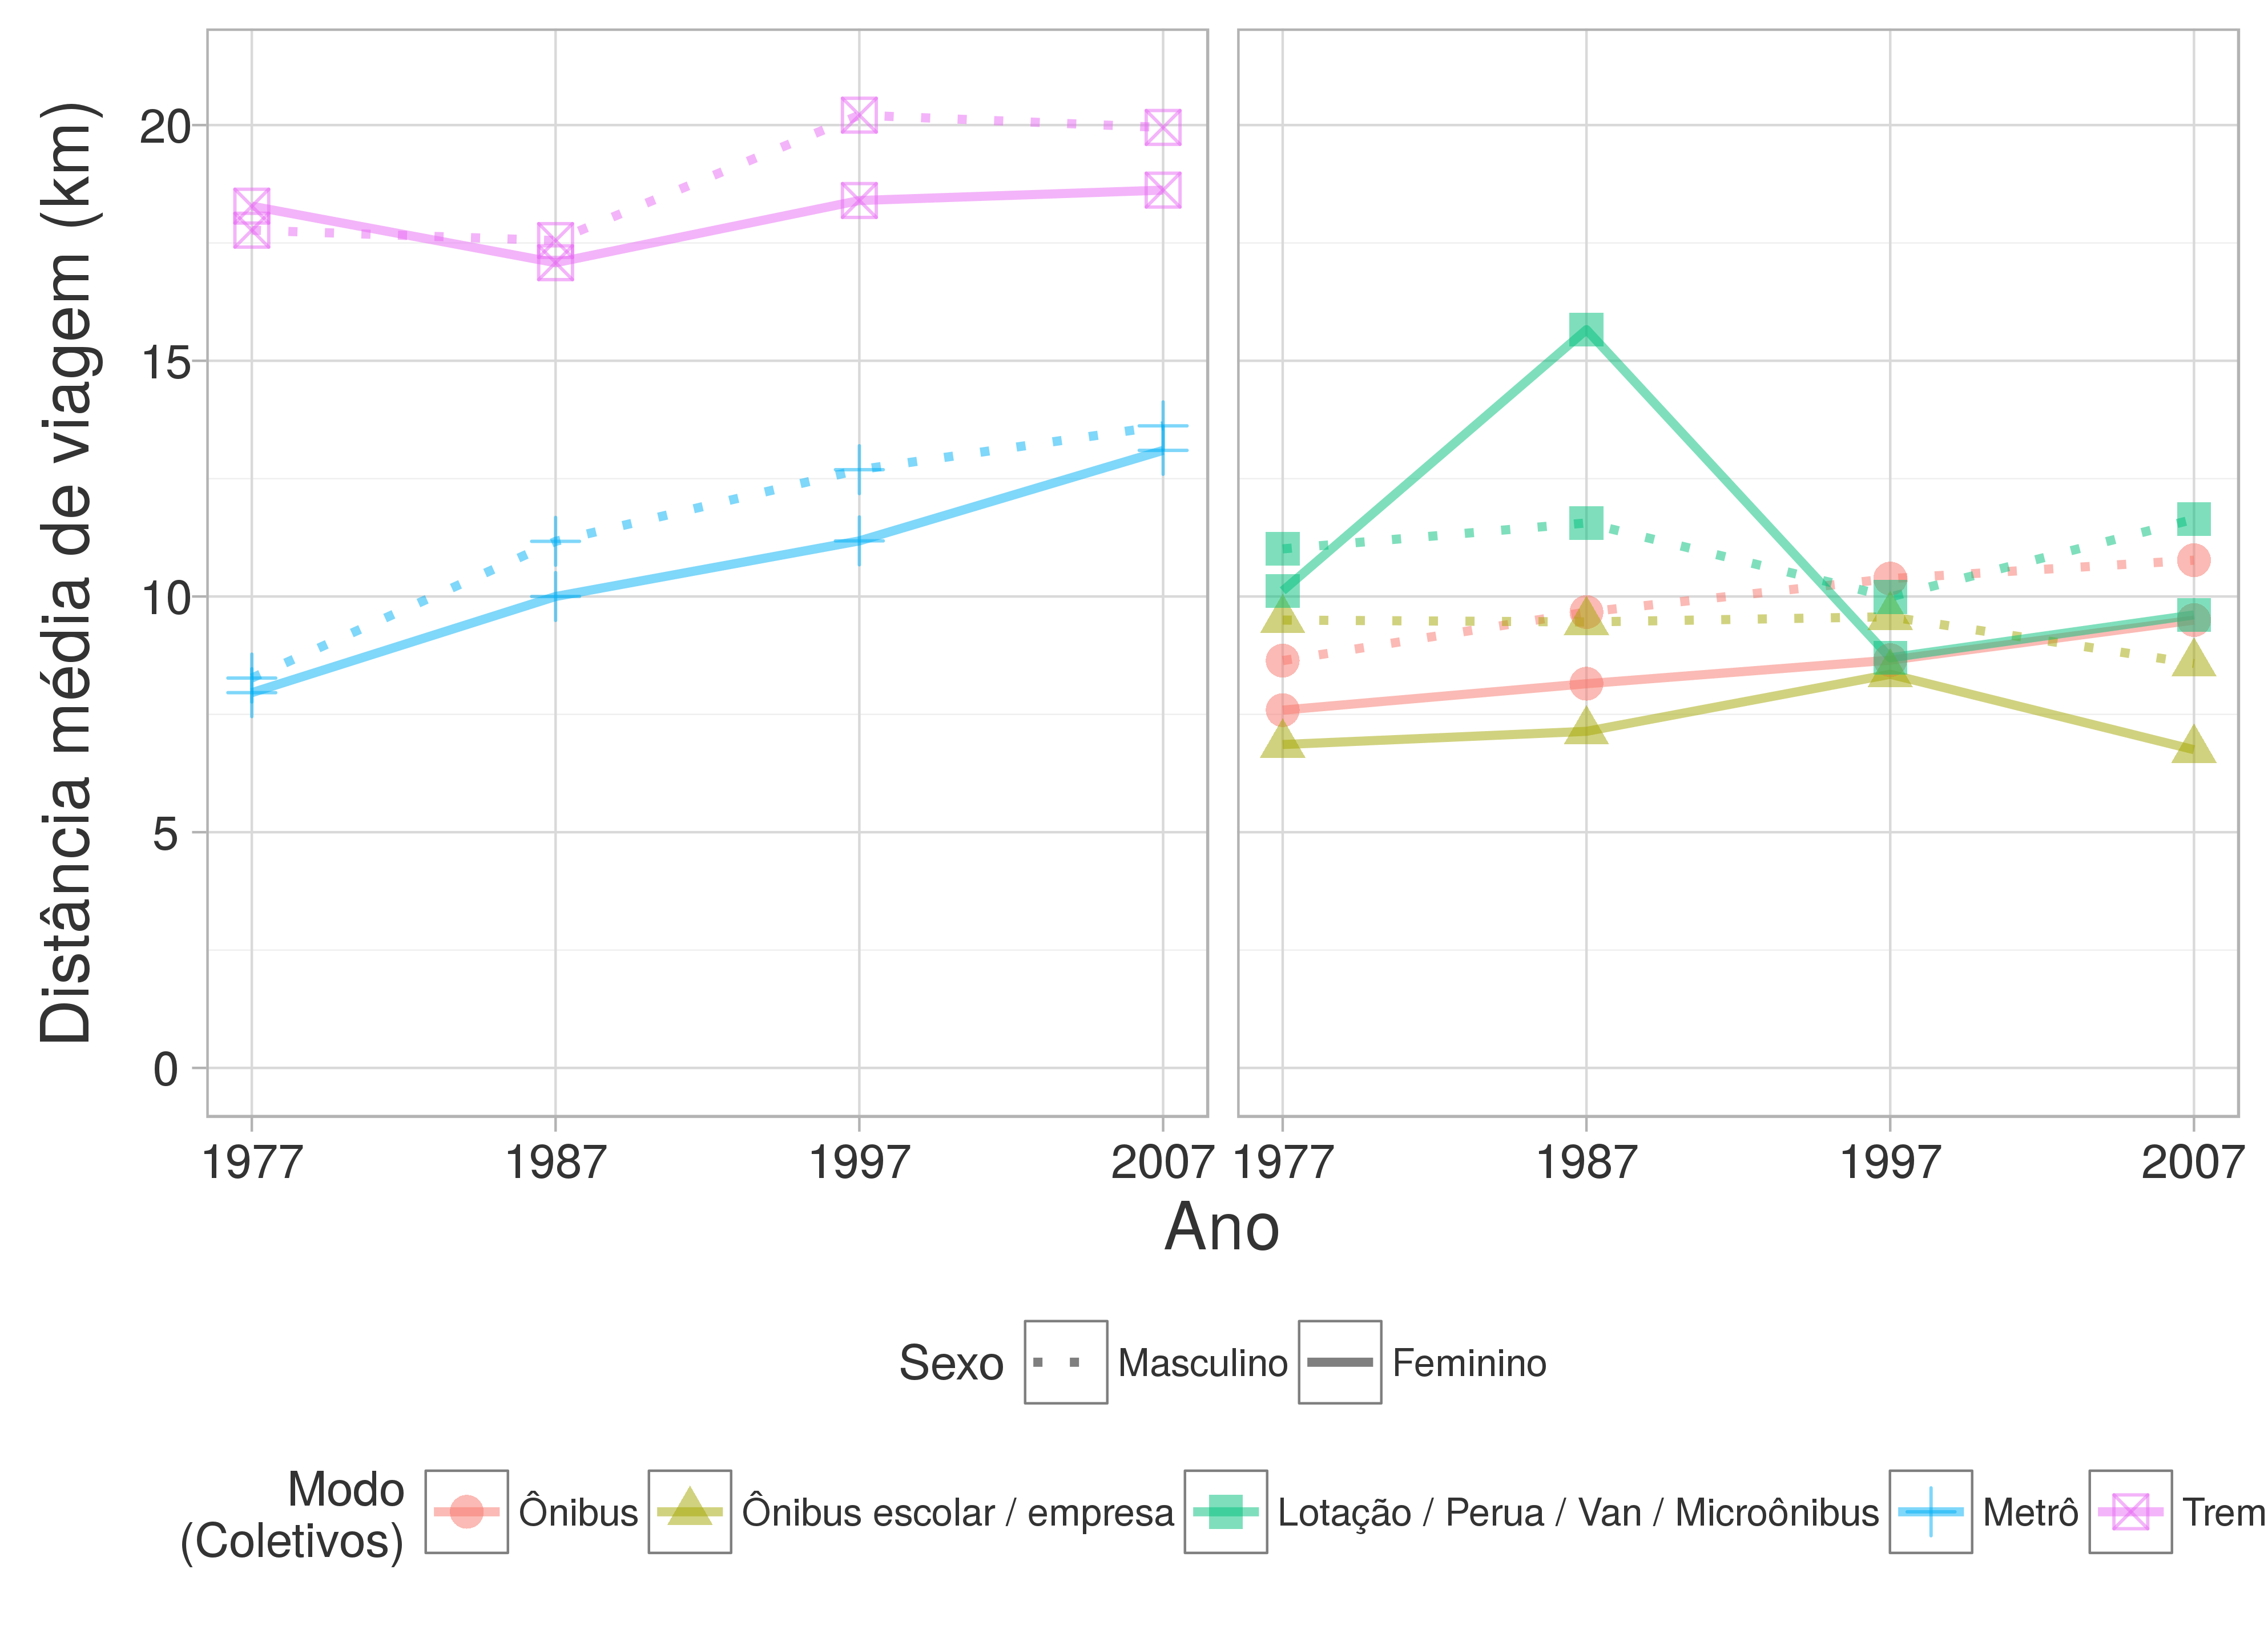
\includegraphics[width=1\textwidth]{./imagens/distancia-coletivo.png}%
    \end{center}%
%    \fonte{Compilação própria}
\end{grafico}%
% Estatísticas para registros com F_VIAG==1 e SEXO
% Expandido com FE_VIAG

\newpage

O Gráfico \ref{graf:distancia-motivo} apresenta as distâncias médias por motivo de viagem (trabalho, educação, servir passageiro, manutenção/compras e lazer/outros), para homens e para mulheres. Verifica-se que:
\begin{compactitem}[]
\item (i) As distâncias médias de viagem motivo trabalho (de natureza compulsória) são superiores a de todos outros motivos. Elas crescem ano a ano: 8,3 km em 1977, 9,2 km em 1987, 9,9 km em 1997 e 10,3 km em 2007.
\item (ii) Para viagens motivo trabalho (natureza compulsória), as distâncias médias femininas são sempre inferiores às masculinas, com diferenças girando em torno de 1,1 km: 0,8 km em 1977, 1,2 km em 1987, 1,3 km em 1977 e 1,0 km em 2007.
\item (iii) As distâncias médias de viagem motivo educação são as mais baixas frente ao demais motivos, exceto em 2007 quando servir passageiro assume média menor. Quando o motivo é escola, as distâncias caem de 1977 (5,44 km) para 1987 (5,23 km), e de 1987 para 1997 (5,16 km). Em 2007, os valores sobem novamente (5,87 km).
\item (iv) Para viagens motivo educação, as distâncias médias femininas são sempre inferiores às masculinas, com diferenças girando em torno de 0,4 km: 0,6 km em 1977, 0,7 km em 1987, 0,3 km em 1977 e, em 2007, a diferença não é estatisticamente significativa.
\item (v) As distâncias médias de viagem motivo manutenção/compras oscilam em torno de 6,9 km: passam de 6,6 km em 1977 para 7,1 km em 1987, caem para 6,9 km em 1997 e sobem novamente para 7,0 km em 2007. 
\item (vi) Para viagens motivo manutenção/compras, as distâncias médias femininas são sempre inferiores às masculinas, com diferenças girando em torno de 1,1 km: 1,1 km em 1977, 0,8 km em 1987, 1,7 km em 1977 e 0,8 km em 2007.
\item (vii) As distâncias médias de viagem motivo lazer/outros oscilam são crescentes no tempo: passam de 6,8 km em 1977 para 7,1 km em 1987, mantém o valor de 7,1 km em 1997 e sobem para 7,3 km em 2007. 
\item (viii) Para viagens motivo lazer/outros, as distâncias médias femininas são sempre inferiores às masculinas, com diferenças girando em torno de 0,9 km: 0,9 km em 1977, 1,2 km em 1987, 1,0 km em 1977 e 0,4 km em 2007.
\item (ix) As distâncias médias de viagem motivo servir passageiro decrescem de 1977 (7,0 km) para 1997 (5,3 km), a partir de quando sobem até 2007 (5,8 km). Lembrando que em 1987 não havia o modo servir passageiro.
\item (x) Para viagens motivo servir passageiro, as distâncias médias femininas são sempre inferiores às masculinas, com diferenças crescentes: 0,1 km em 1977, 0,9 km em 1977 e 1,1 km em 2007.
\end{compactitem}


\begin{grafico}[htb]%
    \caption{\label{graf:distancia-motivo}Distâncias médias de viagem por ano e por sexo, segundo o motivo da viagem}%
    \begin{center}%
        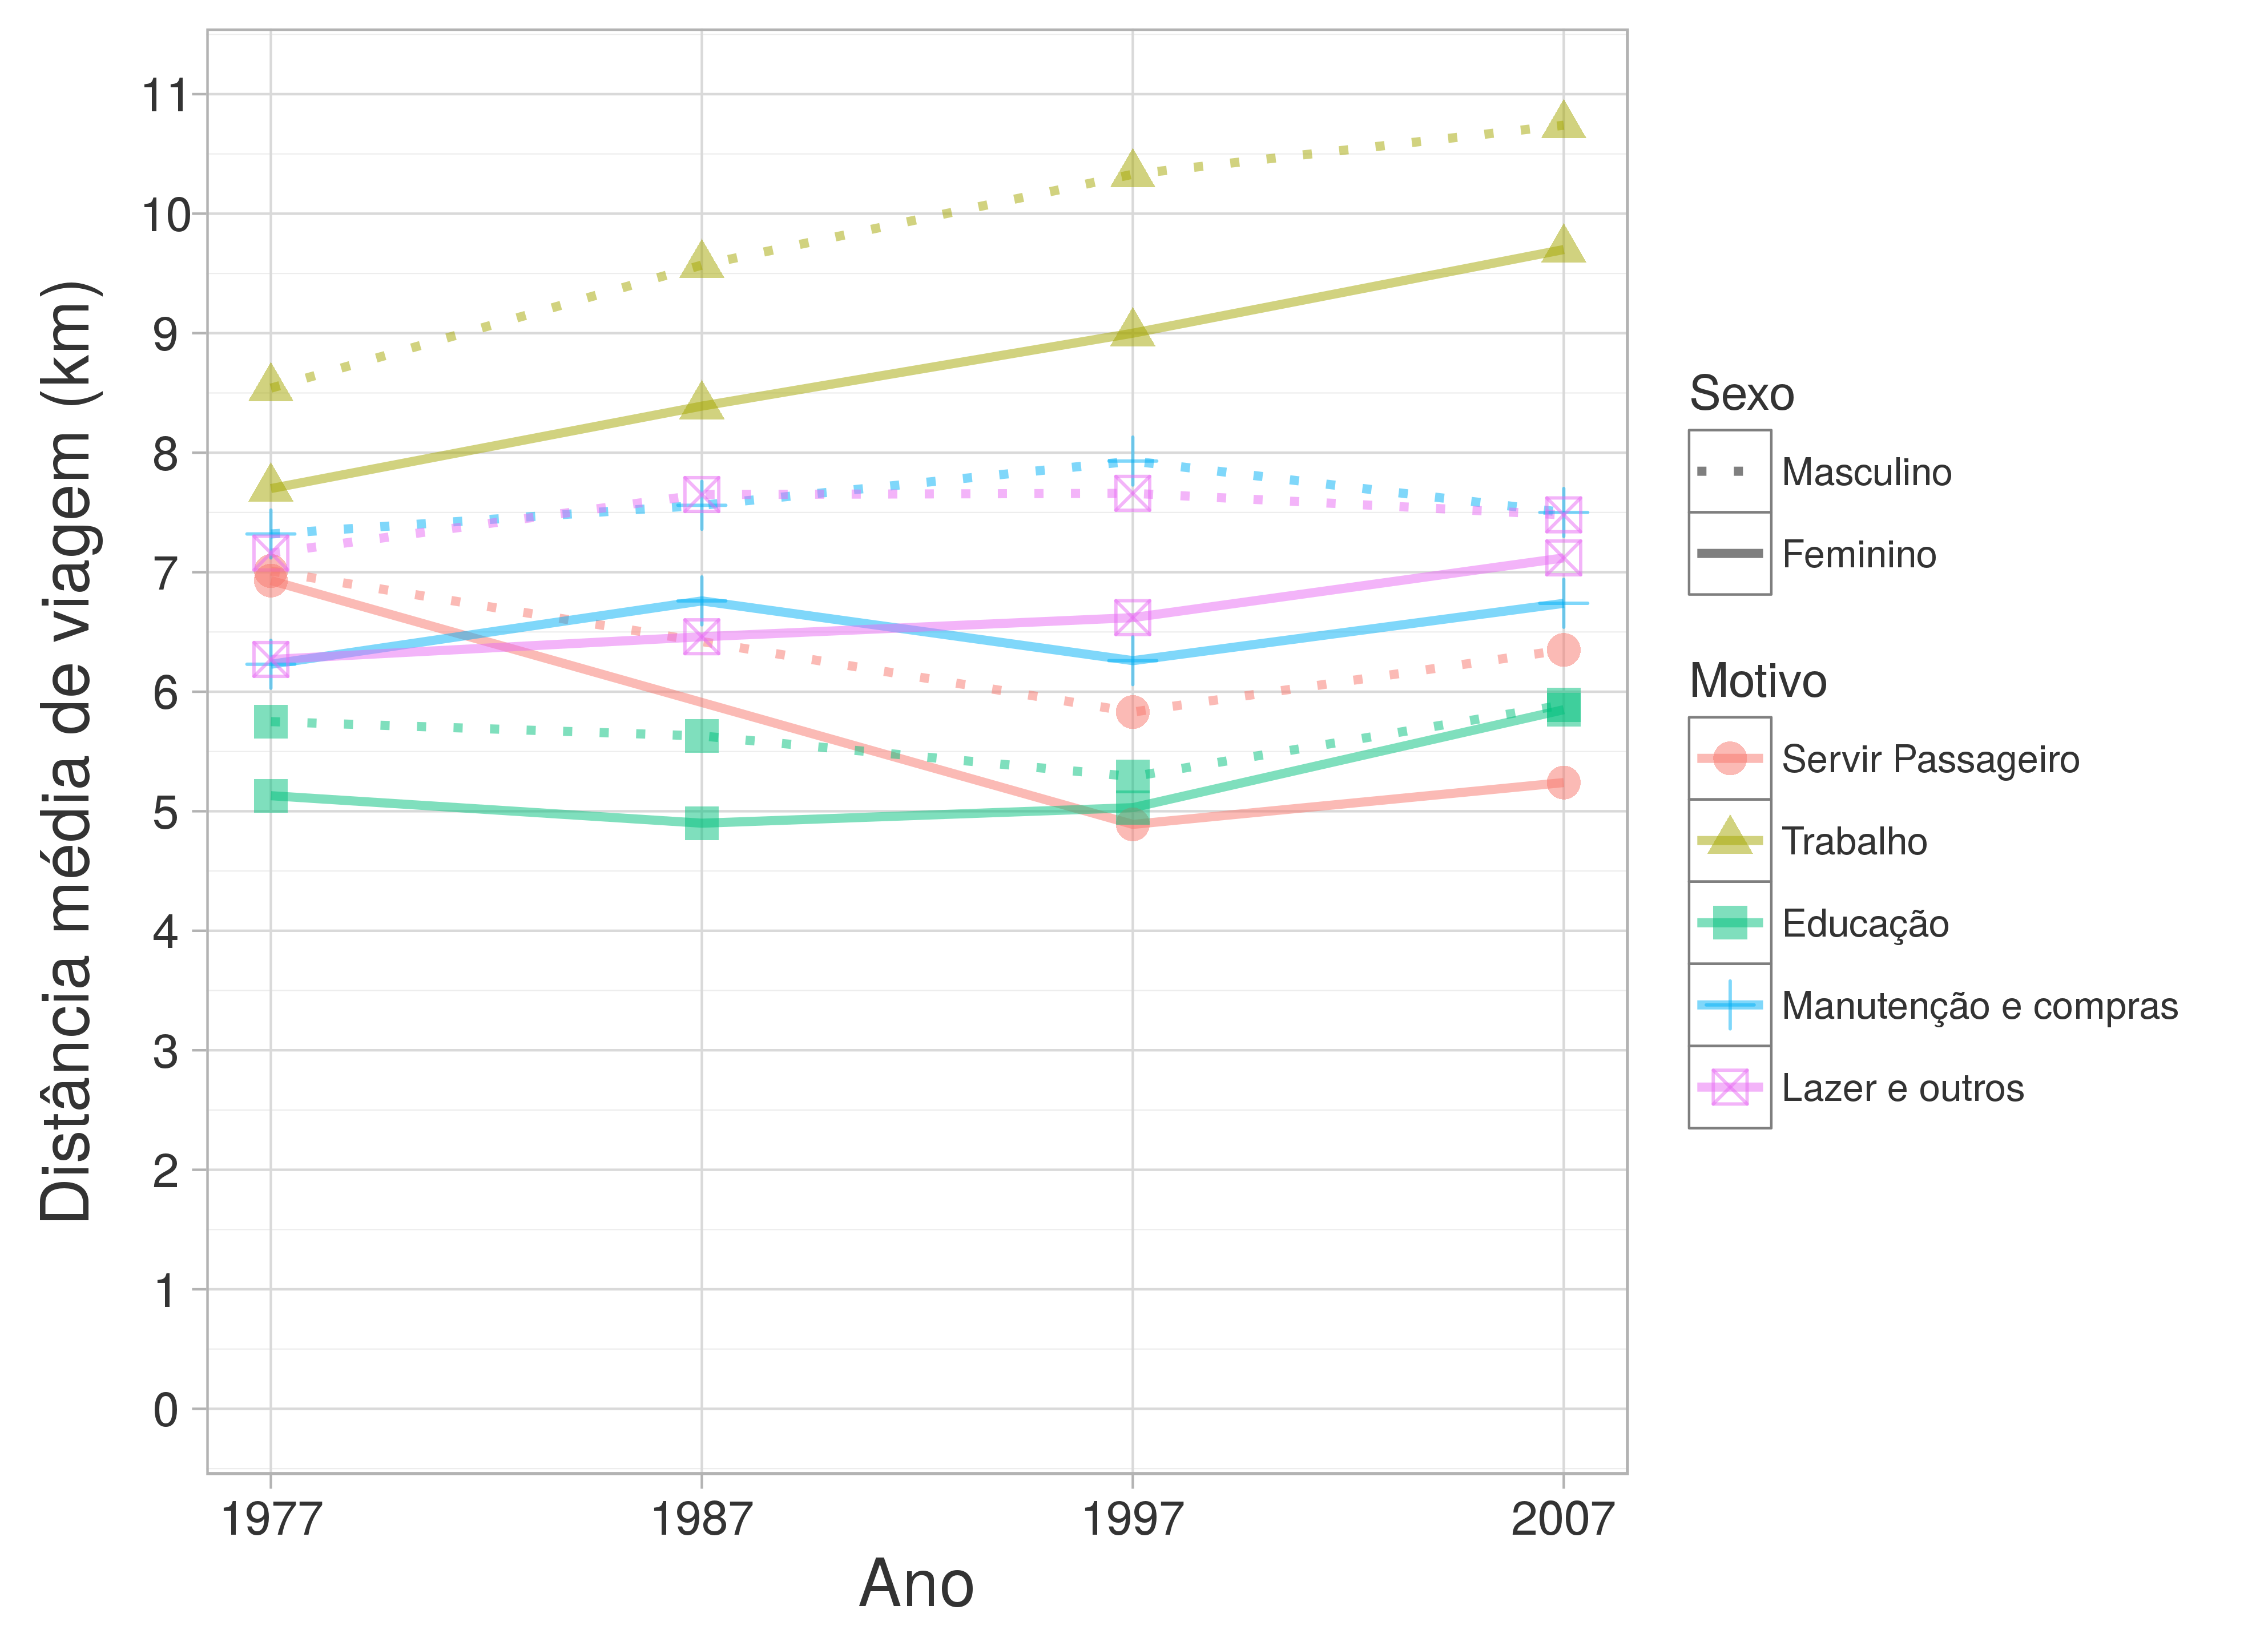
\includegraphics[width=1\textwidth]{./imagens/distancia-motivo.png}%
    \end{center}%
%    \fonte{Compilação própria}
\end{grafico}%
% Estatísticas para registros com F_VIAG==1 e SEXO
% Expandido com FE_VIAG


%TODO -> Fazer estatísticas de PESS_DIST_TOT
%Dalmaso e Strambi (2006) estudaram como o comportamento da distância total viajada por uma pessoa relaciona-se com seus atributos individuais sexo e idade.


\clearpage
\clearpage
\section{Análise de conglomerados para identificação de grupos}\label{sec:analises-clusters}

A análise de conglomerados tem como objetivo segregar elementos (observações) ``em grupos homogêneos internamente, heterogêneos entre si e mutuamente exclusivos, a partir de determinados parâmetros conforme uma medida de similaridade ou distância'' \cite[p.196]{FAVERO2009}.  
Esta técnica estatística de interdependência foi escolhida pois se deseja agrupar as pessoas, ou mesmo famílias, em grupos homogêneos em função da similaridade do comportamento de viagens.

%Vários trabalhos têm usados análises de agrupamento no estudo de XXXXX %TODO
Devido ao tamanho da base de dados e ao baixo desempenho em termos computacionais do pacote  \textit{stats}
\footnote{Também existe a função \textit{agnes}, do pacote \textit{cluster}, cuja documentação está disponível em \url{https://cran.r-project.org/web/packages/cluster/cluster.pdf} e que se propõe a implementar o mesmo algoritmo. Porém, o resultado obtido para os três pacotes (stats, fastcluster e cluster) não foram iguais para o mesmo procedimento. \citeauthoronline{MURTAGH1975} (\citeyear{MURTAGH1975}) já apontavam divergência entre as funções \textit{hclust} e \textit{agnes} quando aplicadas à mesma matriz de distâncias.} \cite{RTEAM2011}, preferiu-se a função \textit{hclust} do pacote \textit{fastcluster}
\footnote{Detalhes da implementação disponível em \citeauthoronline{MULLNER2011} (\citeyear{MULLNER2011}).}. 
Segundo \citeauthoronline{MULLNER2013} (\citeyear{MULLNER2013}), no pior caso, a função do pacote \textit{stats} tem seu tempo de execução proporcional a $N^3$, já a mesma função no pacote \textit{fastcluster}, é poporcional a $N^2$. As análises de conglomerados não hierárquicas foram executadas pela função kmeans do pacote \textit{stats}. Na Figura \ref{fig:roteiro-cluster} pode-se observar os passos realizados nesta etapa de análise.

\begin{figure}[htb]%
    \caption{\label{fig:roteiro-cluster}Etapas para a realização de análise de conglomerados (\textit{clusters})}%
    \begin{center}%
        \includegraphics[width=0.30\textwidth]{./imagens/roteiro-cluster.eps}%
    \end{center}%
%    \fonte{Elaboração própria}
\end{figure}%

\newpage
Na \textbf{etapa A}, foram delimitados dois conjuntos iniciais de variáveis de análise:
\label{conjuntos-variaveis}
\begin{compactitem}
\item \textbf{conjunto I}: De atributos de viagem, relativas à \textbf{família}, a saber: 
\begin{compactitem}[]
\item FAM_DIST_TOT - distância total das viagens da família;
\item FAM_DIST_MED - distância média de viagem da família;
\item FAM_DURACAO_TOT - duração total das viagens da família;
\item FAM_DURACAO_MED - duração média das viagens da família;
\item FAM_VIAG_TOT - número total de viagens da família.
\end{compactitem}
\item \textbf{conjunto II}: De atributos de viagem, relativas à \textbf{pessoa}, a saber: 
\begin{compactitem}[]
\item PESS_DIST_TOT - distância total das viagens da pessoa;
\item PESS_DIST_MED - distância média de viagem da pessoa;
\item PESS_DURACAO_TOT - duração total das viagens da pessoa;
\item PESS_DURACAO_MED - duração média das viagens da pessoa;
\item PESS_MODO_ONIBUS - número de vezes que a pessoa utilizou o ônibus (de linha, escolar, van, etc.);
\item PESS_MODO_DIRIG - número de vezes que a pessoa viajou dirigindo automóvel;
\item PESS_MODO_PASS - número de vezes que a pessoa viajou como passageira de automóvel;
\item PESS_MODO_TREM - número de vezes que a pessoa utilizou o trem ou metrô;
\item PESS_MODO_MOTO - número de vezes que a pessoa utilizou a motocicleta;
\item PESS_MODO_BICI - número de vezes que a pessoa utilizou a bicicleta;
\item PESS_MODO_APE - número de vezes que a pessoa viajou a pé;
\item PESS_MODO_OUTROS - número de vezes que a pessoa utilizou algum outro modo;
\item PESS_NO_MODOS - número de modos diferentes utilizados pela pessoa;
\item PESS_MOTIVO_TRAB - número de viagens da pessoa com motivo trabalho;
\item PESS_MOTIVO_EDUC - número de viagens da pessoa com motivo educação;
\item PESS_MOTIVO_RES - número de viagens da pessoa com motivo residência;
\item PESS_MOTIVO_SERV_PAS - número de viagens da pessoa com motivo servir passageiro;
\item PESS_MOTIVO_MANUT_COMPRAS - número de viagens da pessoa com motivo manutenção/compras;
\item PESS_MOTIVO_LAZER_OUTROS - número de viagens da pessoa com motivo lazer/outros;
\item PESS_NO_MOTIVOS - número de motivos diferentes das viagens da pessoa;
\item PESS_PER_MADRUG - número de viagens da pessoa entre 0h01 e 5h00;
\item PESS_PER_COM_MAN - número de viagens da pessoa entre 5h01 e 9h00;
\item PESS_PER_MANHA - número de viagens da pessoa entre 9h01 e 12h00;
\item PESS_PER_MEIODIA - número de viagens da pessoa entre 12h01 e 14h00;
\item PESS_PER_TARDE - número de viagens da pessoa entre 14h01 e 17h00;
\item PESS_PER_COM_NOI - número de viagens da pessoa entre 17h01 e 22h00;
\item PESS_PER_NOITE - número de viagens da pessoa entre 22h01 e 0h00;
\item PESS_NO_PERIODOS - número de períodos diferentes em que a pessoa realizou viagem;
\item TOT_VIAG  - número total de viagens da pessoa.
\end{compactitem}
\end{compactitem}

Ocorre em diversos bancos de dados, inclusive neste, de se desejar analisar variáveis cujas unidades e ordens de grandezas não são as mesmas.
\citeauthoronline{FARIA2009} (\citeyear{FARIA2009}) indica que há duas razões para padronizar dados: (i) ``evitar que as unidades escolhidas para mensurar as características afetem arbitrariamente a similaridade entre indivíduos'', e (ii) fazer com ``que as características contribuam igualmente na avaliação da similaridade entre indivíduos''. Se houver alguma unidade de medição que tenha uma amplitude maior que as demais (como é o caso das distâncias totais da família em relação à distância média da pessoa), ela terá maior peso na análise de \textit{cluster}. Então, para mitigar o efeito dessas diferenças é indicado padronizar os dados antes de submetê-los à análise de conglomerados. Ao fazer isso, o pesquisador assume que a importância da variável decresce conforme a variabilidade aumenta \cite{EVERITT2011}. Há diversas formas de fazer essa padronização, as mais comuns são \textit{z-scores} e normalização \cite{FAVERO2009}. Há também possibilidades como dividir pela mediana dos desvios absolutos ou pelos intervalos de valores da variável \apud{GNANA1995}{EVERITT2011}, porém, a complexidade deste últimos métodos não se justifica frente ao conjunto de dados em discussão. Assim, na \textbf{etapa B} do presente trabalho, foi feita padronização das variáveis pelo método \textit{z-scores} conforme Equações \eqref{eq:z-score}, \eqref{eq:media} e \eqref{eq:desvio-padrao}.

\begin{equation}\label{eq:z-score}
Z(x)_{i} = \frac{x_{i} - \bar{x}}{\sigma(x)}
\end{equation}
sendo:
\begin{equation}\label{eq:media}
\bar{x} = \frac{1}{n} \sum_{i=1}^{n} x_{i}
\end{equation}

\begin{equation}\label{eq:desvio-padrao}
\sigma(x) = \sqrt{\frac{1}{(n-1)} \sum_{i=1}^{n}(x_{i}-\bar{x})^2 }
\end{equation}

Um dos principais problemas das técnicas de aglomeração não hierárquica \mbox{(K-means)} é definir de início o número de \textit{clusters} desejado \cite{HARTIGAN1985, FAVERO2009, EVERITT2011}. Existem algumas técnicas para essa determinação:

\begin{compactitem}[]
\item (i) A \textbf{\textit{upper tail rule}} que considera os valores de fusão como uma série. Calcula-se a média, desvio padrão, estatística t como o desvio normalizado a partir da média. Em seguida, calcula-se o desvio padrão para cada valor de fusão (assumida distribuição normal), seleciona o primeiro ``significativo'' como sendo aquele cuja estatística t exceda o nível de 5\% de significância. Assim, a hipótese nula é que o valor fusão do k-ésimo termo advém da distribuição normal dos valores de fusão \cite{MOJENA1977}.
\item (ii) O \textbf{índice RMSSTD} (\textit{root mean square standard deviation}), ou raiz quadrada do desvio padrão médio (ver Equação \eqref{eq:RMSSTD}, calcula a homogeneidade dos agrupamentos \cite{SHARMA1996}, de maneira que quanto mais compactos os grupos, menor o valor desta estatística.
 
\begin{equation}\label{eq:RMSSTD} 
RMSSTD = \sqrt{\frac{\displaystyle\sum_{\substack{i=1\\
j=1}}^{\substack{nc\\
d}}\displaystyle\sum_{k=1}^{n_{j}}(x_{k}-\bar{x}_{j})^2}{\displaystyle\sum_{\substack{i=1\\
j=1}}^{\substack{nc\\
d}}(n_{ij}-1)}}
\end{equation}

\item (iii) O \textbf{índice $R^2$ ajustado} (ver Equação \eqref{eq:RS}), indica dissimilaridade entre agrupamentos \cite{SHARMA1996}, assim, quanto mais alto o valor de $R^2$ ajustado, mais dissimilaridade existe entre os grupos. O pesquisador pode estabelecer um valor desejado para $R^2$ e, a partir daí, determinar o número de \textit{clusters}.

\begin{equation}\label{eq:RS} 
R^2 = \frac{\left[\displaystyle\sum_{\substack{i=1\\
j=1}}^{\substack{nc\\
d}}\sum_{k=1}^{n_{j}}(x_{i}-\bar{x}_{j})^2\right]-\left[\displaystyle\sum_{\substack{i=1\\
j=1}}^{\substack{nc\\
d}}\displaystyle\sum_{k=1}^{n_{ij}}(x_{k}-\bar{x}_{j})^2\right]}{\displaystyle\sum_{j=1}^{d}\displaystyle\sum_{k=1}^{n_{j}}(x_{k} - \bar{x}_{j})^2 }
\end{equation}

\item (iv) O \textbf{\textit{best cut}} é um método que se baseia em um dendrograma (representação bidimensional em forma de árvore) que deve ser cortado quando as diferenças entre grupos forem visualmente mais significativas. Nesta representação, as linhas são ligadas segundo níveis de similaridade que agregará os indivíduos \cite{EVERITT2011}.
\end{compactitem}

Então, primeiro foi realizada a aglomeração hierárquica para definir as quantidades de grupos.
No método hierárquico, se há n observações (linhas), parte-se de n grupos, ou seja, existe uma observação por grupo. 
A partir de medidas de similaridade, num processo iterativo, as observações vão sendo agrupadas até que se chegue a um único grupo no final. 
Segundo \citeonline{MAXWELL1977}, primeiro é feita a conversão da matriz \textit{n versus p} de dados em uma matriz \textit{n versus n} de medidas de similaridade ou dissimilaridade, tendo-se \textit{n} unidades amostrais e \textit{p} características.
Optou-se por primeiro utilizar o \textbf{\textit{best cut}} com os dendrogramas%
\footnote{Os dendrogramas gerados admitiram escala não-monotônica.} 
e, em seguida, seriam avaliados os índices \textbf{RMSSTD} e \textbf{$R^2$ ajustado}.

As medidas de (dis)similaridade podem ser de distância, correlação ou associação, esta última indicada para variáveis qualitativas. Como as variáveis selecionadas na \textbf{etapa A} são métricas ou \textit{dummies}, são indicadas medidas de distância ou correlação. 
Na Tabela \ref{tab:dist-cluster} é possível observar algumas das principais medidas de dissimilaridade comumente utilizadas.
Optou-se, na \textbf{etapa C}, pela medida de distância euclidiana, indicada pela literatura \apud{HAIR2005}{FAVERO2009}, 
a ser adotada em conjunto com os métodos de agrupamento Ward \cite{WARD1963} e centroide. O arcabouço teórico indica que tanto as distâncias euclidianas quanto as euclidianas quadráticas resultarão nos mesmos \textit{clusters} e, no caso da função \textit{hclust} utilizada, a distância padrão calculada é a euclidiana.



\begin{table}[htb]
    \IBGEtab{
	    \renewcommand{\arraystretch}{2.8}
        \caption{Medidas de dissimilaridade utilizadas em análise de \textit{cluster}}
		\label{tab:dist-cluster}
    }{%
	    \begin{tabular}{ll}
        \toprule
		    \headerTabCenterCell{Medida} &
	   	    \headerTabCenterCell{Fórmula}\\
		    \midrule \midrule
						Distância Euclidiana &
						\begin{math}
						    d_{ij}=\left[\displaystyle\sum_{k=1}^{p}w_{k}^2(x_{ik}-x_{jk})^2\right]^{1/_2}
						\end{math} \\
		    %\midrule
						Distância \textit{city block} &
						\begin{math}
                d_{ij}=\displaystyle\sum_{k=1}^{p}w_{k}|x_{ik}-x_{jk}|
						\end{math} \\
				%\midrule
				    Distância de Minkowski &
				    \begin{math}
				        d_{ij}=\left(\displaystyle\sum_{k=1}^{p}w_{k}^{r}|x_{ik}-x_{jk}|^{r}\right)^{{}1/_r} \quad (r\geq1)
				    \end{math} \\
				%\midrule
				    Distância de Canberra &
				    \begin{math}
				        d_{ij}= \begin{cases}
				                  0 & \quad \text{for } x_{ik}=x_{jk}=0 \\
				                  \displaystyle\sum_{k=1}^{p}w_{k}|x_{ik}-x_{jk}|/(|x_{ik}|+|x_{jk}|) & \quad \text{for } x_{ik} \neq 0 \text{ or } x_{jk} \neq 0\\
				                \end{cases}
				    \end{math} \\
			\bottomrule	
		\end{tabular}
    }{%
		\fonte{\cite{EVERITT2011}}
		}
\end{table}

Na \textbf{etapa D}, foi feita a aglomeração para o \textbf{conjunto I} de variáveis da família e para o \textbf{conjunto II} de variáveis da pessoa, utilizando tanto o método Ward quanto o centroide, utilizando filtros que captassem a ocorrência da família (F_FAM=1) ou da pessoa (F_PESS=1), respectivamente, para que não houvesse repetição indevida de famílias ou pessoas. Essas aglomerações foram feitas sem distinção dos anos e resultaram nos dendrogramas apresentados nas Figuras \ref{fig:cluster-fam-total} e \ref{fig:cluster-pess-total}. Percebe-se que a forma do dendrograma difere muito pouco entre os métodos Ward e centroide para o mesmo conjunto de variáveis.
%Para as análises seguintes foi escolhido o centroide pois segundo \apudonline{HAIR2005}{FAVERO2009}  “este método é mais robusto para observações atípicas”. 

Considerando o \textbf{best cut} observa-se que os dendrogramas que partiram das variáveis de família, indicam 4 como sendo um número de \textit{clusters} interessante de ser dado como \textit{input} do método K-means - observar seções S da Figura \ref{fig:cluster-fam-total}. Os índices \textbf{RMSSTD} e \textbf{$R^2$} ajustado, conforme pode ser visto no Gráfico \ref{graf:rmsstd-r2-cluster-fam-total}, também corroboram para a divisão em 4 grupos, representando 90\% da variância.

Partindo do conjunto de atributos de viagens relativas às pessoas, o \textbf{best cut} dos dendrogramas resultantes também indicam 4 \textit{clusters}, seja pelo método Ward, seja pelo centroide - observar seções S da Figura \ref{fig:cluster-pess-total}. Os índices \textbf{RMSSTD} e \textbf{$R^2$} ajustado, conforme pode ser visto no Gráfico \ref{graf:rmsstd-r2-cluster-pess-total}, também corroboram para a divisão em 4 grupos, representando mais de 90\% da variância.

\begin{figure}[htb]%
    \caption{\label{fig:cluster-fam-total}Dendrograma resultante da análise de conglomerados hierárquico, para o conjunto de atributos de viagens relativas às famílias}%
    \begin{center}%
        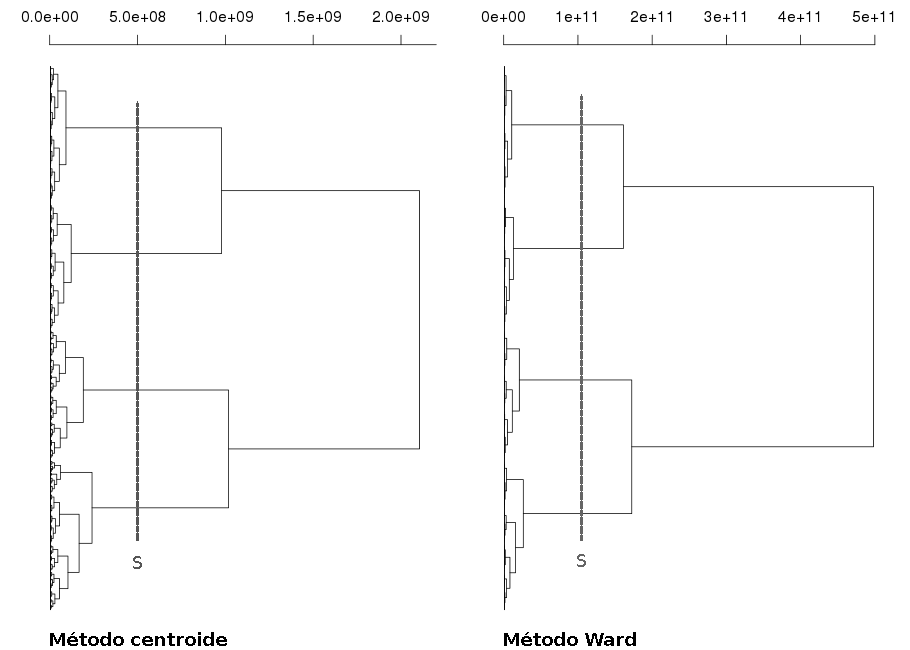
\includegraphics[width=0.85\textwidth]{./imagens/dendro-hierarq-cluster-familia-total-final.png}%
    \end{center}%
%    \fonte{Elaboração própria}
\end{figure}%

\begin{grafico}[htb]%
    \caption{\label{graf:rmsstd-r2-cluster-fam-total}Avaliação do número de \textit{clusters} para o conjunto de atributos de viagens relativas às famílias}%
    \begin{center}%
        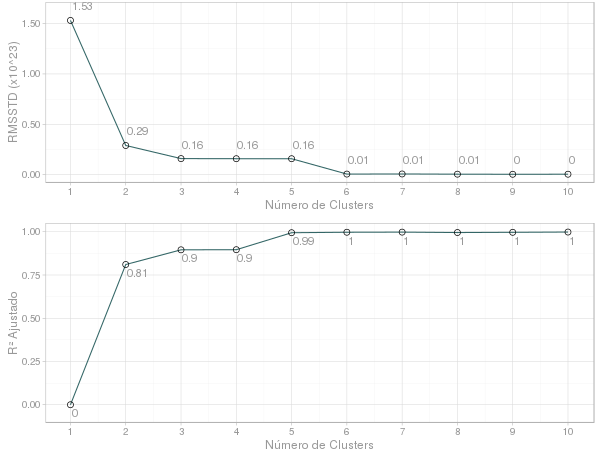
\includegraphics[width=0.8\textwidth]{./imagens/No-clusters-R2-RMSSTD-familia.png}%
    \end{center}%
%    \fonte{Elaboração própria}
\end{grafico}%

\clearpage
\begin{figure}[htb]%
    \caption{\label{fig:cluster-pess-total}Dendrograma resultante da análise de conglomerados hierárquico, para o conjunto de atributos de viagens relativas às pessoas}%
    \begin{center}%
        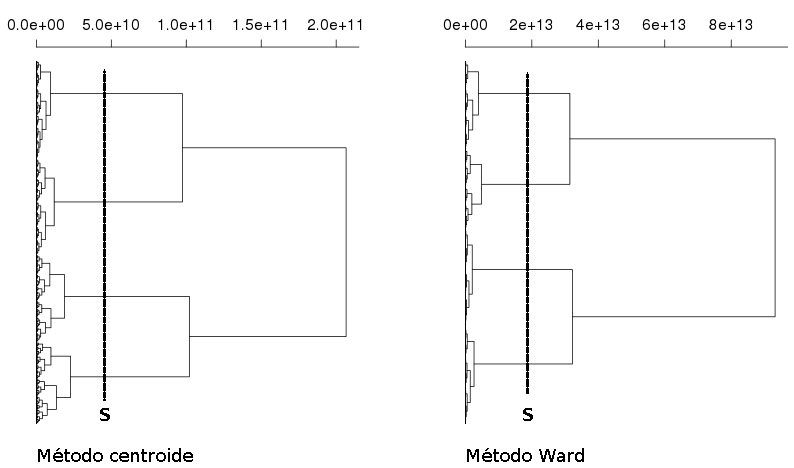
\includegraphics[width=0.8\textwidth]{./imagens/dendro-hierarq-cluster-pessoa-total-final.png}%
    \end{center}%
%    \fonte{Elaboração própria}
\end{figure}%

\begin{grafico}[htb]%
    \caption{\label{graf:rmsstd-r2-cluster-pess-total}Avaliação do número de \textit{clusters} para o conjunto de atributos de viagens relativas às pessoas}%
    \begin{center}%
        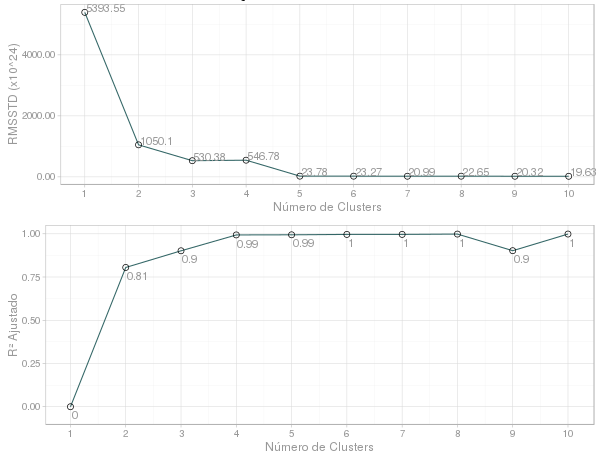
\includegraphics[width=0.77\textwidth]{./imagens/No-clusters-R2-RMSSTD-pessoas.png}%
    \end{center}%
%    \fonte{Elaboração própria}
\end{grafico}%

\clearpage
Assim, na \textbf{etapa E}, definiu-se que seriam adotados 4 \textit{clusters}, tanto para o conjunto de variáveis I (de família) como o II (de pessoas) no método de aglomeração K-means%
\footnote{ A função \textit{kmeans} do pacote \textit{stats} do software R implementa o algoritmo de \citeonline{HARTIGAN1979} por padrão para sua execução, que utiliza também a distância euclidiana como medida de similaridade.} 
que, segundo \apudonline{GOUVEA2006}{FAVERO2009}, minimiza a variância interna aos grupos e maximiza a variância entre grupos.

Na \textbf{etapa F}, foram formados então quatro agrupamentos para atributos de viagens de \textbf{família}, pelo método Ward. Observa-se que os grupos formados correspondem exatamente às observações de cada ano. 
Ou seja, o \textit{cluster} 1 agregou as observações de 1977, o \textit{cluster} 2 agregou as observações de 1987, e assim por diante - ver Tabela \ref{tab:cluster-fam-ward-4}. Entretanto, utilizando o método centroide, houve a união de 1997 e 2007, além da separação de 1987 em dois grupos distintos - ver Tabela \ref{tab:cluster-fam-centroide-4}.
Ao analisar os quatro agrupamentos para atributos de viagens de \textbf{pessoas}, tanto o método centroide quanto o Ward, formam grupos que correspondem exatamente às observações de cada ano, como na Tabela \ref{tab:cluster-fam-ward-4}.

\begin{table}[htb]
    \IBGEtab{%\renewcommand{\arraystretch}{1.5}%%\ABNTEXfontereduzida%
%	    \renewcommand{\arraystretch}{1.5}
        \caption{Resultado do agrupamento de 4 \textit{clusters}, por atributos de viagens de família - método Ward}
		\label{tab:cluster-fam-ward-4}
    }{%
	    \begin{tabular}{ccccc}
            \toprule
	             \headerTabCenterCell{\quebraLinhaCel{\textit{Cluster}\\nº}} &
   	           \headerTabCenterCell{\quebraLinhaCel{\% de famílias\\de 1977}} &
   	           \headerTabCenterCell{\quebraLinhaCel{\% de famílias\\de 1987}} &   	           
   	           \headerTabCenterCell{\quebraLinhaCel{\% de famílias\\de 1997}} &   	           
   	           \headerTabCenterCell{\quebraLinhaCel{\% de famílias\\de 2007}}\\
		    \midrule \midrule
				1& % É  o 2, na verdade
		    	100&
		    	0&
		    	0&
				0\\
			\hline
				2& % É o 1, na verdade
				0&
				100&
				0&
		        0\\
			\hline
				3& % É o 3 mesmo
				0&
				0&
				100&
		        0\\
			\hline
				4& % È o 4 mesmo
				0&
				0&
				0&
		        100\\
			\bottomrule	
		\end{tabular}
    }{%
		%\fonte{Elaboração própria}
	}
\end{table}

\begin{table}[htb]
    \IBGEtab{%\renewcommand{\arraystretch}{1.5}%%\ABNTEXfontereduzida%
	    \renewcommand{\arraystretch}{1.5}
        \caption{Resultado do agrupamento de 4 \textit{clusters}, por atributos de viagens de família - método centroide}
		\label{tab:cluster-fam-centroide-4}
    }{%
	    \begin{tabular}{ccccc}
            \toprule
	             \headerTabCenterCell{\quebraLinhaCel{\textit{Cluster}\\nº}} &
   	           \headerTabCenterCell{\quebraLinhaCel{\% de famílias\\de 1977}} &
   	           \headerTabCenterCell{\quebraLinhaCel{\% de famílias\\de 1987}} &   	           
   	           \headerTabCenterCell{\quebraLinhaCel{\% de famílias\\de 1997}} &   	           
   	           \headerTabCenterCell{\quebraLinhaCel{\% de famílias\\de 2007}}\\
		    \midrule \midrule
				1 & % É  o 3, na verdade
		    	100 &
		    	0 &
		    	0 &
				0\\
			\hline
				2 & % É o 1, na verdade
				0 &
				100 &
				0 &
		        0\\
			\hline
				3 & % É o 2, na verdade
				0 &
				100 &
				0 &
		        0\\
			\hline
				4 & % È o 4 mesmo
				0 &
				0 &
				51,94 &
		        48,06\\
			\bottomrule	
		\end{tabular}
    }{%
		\nota{Do total de famílias de 1987, 55,6\% pertencem ao grupo 2 e 44,4\% pertencem ao grupo 3.}
	}
\end{table}

\newpage
Foi feita uma nova análise, agora com três agrupamentos, tendo em foco a \textbf{família}, para observar quais grupos se juntariam e quais continuariam separados. 
Pelo método Ward, os grupos que se unem são os anos de 1997 e 2007. 
Já pelo método centroide, 1997 destaca-se de 2007, enquanto 1987 se agrega completamente a 1977, conforme pode ser observado nas Tabelas \ref{tab:cluster-fam-ward-3} e \ref{tab:cluster-fam-centroide-3}. 

\begin{table}[htb]
    \IBGEtab{%\renewcommand{\arraystretch}{1.5}%%\ABNTEXfontereduzida%
	    \renewcommand{\arraystretch}{1.5}
        \caption{Resultado do agrupamento de 3 \textit{clusters}, por atributos de viagens de família - método Ward}
		\label{tab:cluster-fam-ward-3}
    }{%
	    \begin{tabular}{ccccc}
            \toprule
	             \headerTabCenterCell{\quebraLinhaCel{\textit{Cluster}\\nº}} &
   	           \headerTabCenterCell{\quebraLinhaCel{\% de famílias\\de 1977}} &
   	           \headerTabCenterCell{\quebraLinhaCel{\% de famílias\\de 1987}} &   	           
   	           \headerTabCenterCell{\quebraLinhaCel{\% de famílias\\de 1997}} &   	           
   	           \headerTabCenterCell{\quebraLinhaCel{\% de famílias\\de 2007}}\\
		    \midrule \midrule
				1 &
		    	100 &
		    	0 &
		    	0 &
				0\\
			\hline
				2 &
				0 &
				100 &
				0 &
		        0\\
			\hline
				3 & % É o 3 mesmo
				0 &
				0 &
				46,5 &
		        53,5\\
			\bottomrule	
		\end{tabular}
    }{%
		%\fonte{Elaboração própria}
	}
\end{table}

\begin{table}[htb]
    \IBGEtab{%\renewcommand{\arraystretch}{1.5}%%\ABNTEXfontereduzida%
	    \renewcommand{\arraystretch}{1.5}
        \caption{Resultado do agrupamento de 3 \textit{clusters}, por atributos de viagens de família - método centroide}
		\label{tab:cluster-fam-centroide-3}
    }{%
	    \begin{tabular}{ccccc}
            \toprule
	             \headerTabCenterCell{\quebraLinhaCel{\textit{Cluster}\\nº}} &
   	           \headerTabCenterCell{\quebraLinhaCel{\% de famílias\\de 1977}} &
   	           \headerTabCenterCell{\quebraLinhaCel{\% de famílias\\de 1987}} &   	           
   	           \headerTabCenterCell{\quebraLinhaCel{\% de famílias\\de 1997}} &   	           
   	           \headerTabCenterCell{\quebraLinhaCel{\% de famílias\\de 2007}}\\
		    \midrule \midrule
				1 &
		    	48,1 &
		    	51,9 &
		    	0 &
				0\\
			\hline
				2 &
				0 &
				0 &
				100 &
		        0\\
			\hline
				3 &
				0 &
				0 &
				0 &
		        100\\
			\bottomrule	
		\end{tabular}
    }{%
		%\fonte{Elaboração própria}
	}
\end{table}

Ao focar os atributos de viagens das \textbf{pessoas}, agrupadas em três \textit{clusters}, não houve diferença no resultado utilizando Ward ou centroide, tal como ocorreu com quatro grupos,  conforme Tabela \ref{tab:cluster-pess-ward-centroide-3}. 
Nota-se que 1977 e 1987 se mantêm separados, e 1997 se une a 2007. 
    
\begin{table}[htb]
    \IBGEtab{%\renewcommand{\arraystretch}{1.5}%%\ABNTEXfontereduzida%
	    \renewcommand{\arraystretch}{1.5}
        \caption{Resultado do agrupamento de 3 \textit{clusters}, por atributos de viagens de pessoas - métodos Ward e centroide}
		\label{tab:cluster-pess-ward-centroide-3}
    }{%
	    \begin{tabular}{ccccc}
            \toprule
	             \headerTabCenterCell{\quebraLinhaCel{\textit{Cluster}\\nº}} &
   	           \headerTabCenterCell{\quebraLinhaCel{\% de famílias\\de 1977}} &
   	           \headerTabCenterCell{\quebraLinhaCel{\% de famílias\\de 1987}} &   	           
   	           \headerTabCenterCell{\quebraLinhaCel{\% de famílias\\de 1997}} &   	           
   	           \headerTabCenterCell{\quebraLinhaCel{\% de famílias\\de 2007}}\\
		    \midrule \midrule
				1 &
		    	100 &
		    	0 &
		    	0 &
				0\\
			\hline
				2 &
				0 &
				100 &
				0 &
		        0\\
			\hline
				3 &
				0 &
				0 &
				51,9 &
		        48,1\\
			\bottomrule	
		\end{tabular}
    }{%
		%\fonte{Elaboração própria}
	}
\end{table}

Os resultados mostram que a variável ANO, embora não inserida nas análises de conglomerados, acabou sendo a grande diferenciadora dos grupos.
Esses resultados levantam questões como:
\begin{compactitem}[]
\item (i) o tempo (em si ou como \textit{proxy} de outras variáveis) é uma categoria de análise relevante;
\item (ii) pode ter havido alterações no método de pesquisa (conceitos, definições, categorias de variáveis, etc.) e o agrupamento temporal esteja captando este efeito; 
\item (iii) deve haver semelhanças entre 2007 e 1997;
\item (iv) deve haver semelhanças entre 1987 e 1977, talvez mais fracas que aquelas entre 2007 e 1997.
\end{compactitem}

Sob a perspectiva de gênero, retomando os dados de participação das mulheres na PEA, apresentados no Gráfico \ref{graf:evolucao-pea} (página \pageref{graf:evolucao-pea}), percebe-se o $\Delta_{1991-1980} = 6,3\%$, $\Delta_{2000-1991} = 11,2\%$ e $\Delta_{2010-2000} = 4,8\%$. 
Embora, os dados da PEA refiram-se aos anos 1980, 1991, 2000 e 2010, não coincidentes com os das Pesquisas OD (1977, 1987, 1997 e 2007), se tomarmos os anos mais próximos como referencial de análise, percebemos que o maior salto na participação feminina no mercado de trabalho ocorreu entre 1991 e 2000, e que as pesquisas que parecem apresentar a maior dissemelhança são as OD-1987 e OD-1997. 
Não é possível fazer muitas afirmações a partir somente deste paralelo, entretanto, isto pode ser um indicativo de que os padrões de mobilidade se alteraram sob efeito do tempo e também considerando o gênero como categoria de análise.
 
Para explorar melhor o que ocorre dentro de cada grupo e as diferenças entre grupos foram analisadas as características de viagens, das pessoas e das famílias dos quatro \textit{clusters} resultantes - ver Anexo \ref{chap:anexo_4_clusters_td}.

No agrupamento feito por atributos de viagens da \textbf{família} pelo método \textbf{Ward}, observa-se que a maior diferença percentual entre valores mínimo e máximo entre grupos ocorreu com a variável ``\% de pessoas com superior completo'' (76\%) e a menor diferença ocorreu com a variável ``sexo'' (4\%).
Se por um lado já se esperava que o grau de instrução fosse uma variável relevante para explicar o comportamento da demanda, por outro, contrariando expectativas iniciais, a variável sexo sozinha não se mostrou tão relevante assim.
A Tabela \ref{tab:cluster-fam-ward-top10} apresenta as variáveis que apresentaram as diferenças percentuais entre valores máximos e mínimos superiores a 50\%.
Para estas nove variáveis foi realizado teste qui-quadrado de Pearson (de independência) em relação à variável ``nº do \textit{cluster}'' e todas mostraram-se significativas considerando com um nível de significância de 5\%. 

\begin{table}[htb]
    \IBGEtab{%\renewcommand{\arraystretch}{1.5}%%\ABNTEXfontereduzida%
	    \renewcommand{\arraystretch}{1.5}
        \caption{Ordenamento das variáveis pelas maiores diferenças percentuais - para agrupamento FAM_CLUSTER_WARD4}
		\label{tab:cluster-fam-ward-top10}
    }\\
		    \midrule \midrule
		    	1º&
				\% de pessoas com superior completo& 
				76\\
			\hline
				2º& 
				\% de pessoas com situação familiar `outros'&
		        71\\
			\hline
				3º& 
				\% de famílias na Classe A&
		        67\\		        
			\hline
				4º& 
				\% de pessoas com médio completo ou superior incompleto&
		        66\\	
			\hline
				5º& 
				\% de pessoas que servem passageiro no destino&
		        65\\			        
			\hline
				6º& 
				\% de famílias na Classe E&
		        61\\
			\hline
				7º& 
				\% de famílias com presença de criança entre 0 e 4 anos&
		        60\\
			\hline
				8º& 
				\% de pessoas com situação familiar `empregado(a)'&
		        59\\
			\hline
				9º&
				\% de famílias com presença de criança entre 5 e 9 &
		        56\\
			\bottomrule	
		\end{tabular}
    }{%
		%\fonte{Elaboração própria}
	}
\end{table}

No agrupamento feito por atributos de viagens da \textbf{família} pelo método \textbf{centroide}, observa-se que a maior diferença percentual entre valores mínimo e máximo entre grupos ocorreu com a variável ``\% de famílias na Classe A'' (79\%) e a menor diferença ocorreu com a variável ``Média da quantidade de trabalhadores (as) na família'' (2\%).

Buscando entender o fato curioso de 1987 ter se dividido entre dois grupos quando da formação de quatro grupos com método centroide (Tabela \ref{tab:cluster-fam-centroide-4}), foram levantadas as maiores diferenças percentuais entre valores mínimo e máximo (ver Anexo \ref{chap:anexo_4_clusters_td}) que ocorreram entre os grupos 2 e 3 de 1987. 
Estas principais diferenças eram de categorias relacionadas à \textbf{distância}, \textbf{sexo} e \textbf{situação familiar}, a saber:
\begin{compactitem}[]
\item (i) distâncias médias de viagem (da pessoa e da família); 
\item (ii) \% de pessoas do sexo feminino e 
\item (iii) \% de outros parentes / agregados.
\end{compactitem}

A Tabela \ref{tab:cluster-fam-centr-top10} apresenta as variáveis que apresentaram as diferenças percentuais entre valores máximos e mínimos superiores a 50\%.
Para estas nove variáveis foi realizado teste qui-quadrado de Pearson (de independência) em relação à variável ``nº do \textit{cluster}'' e todas mostraram-se significativas considerando um nível de significância de 5\%. 

\begin{table}[htb]
    \IBGEtab{%\renewcommand{\arraystretch}{1.5}%%\ABNTEXfontereduzida%
	    \renewcommand{\arraystretch}{1.5}
        \caption{Ordenamento das variáveis pelas maiores diferenças percentuais - para agrupamento FAM_CLUSTER_CENTROIDE4}
		\label{tab:cluster-fam-centr-top10}
    }\\
		    \midrule \midrule
				1º& 
				\% de famílias na Classe A&
		        79\\		        
			\hline
				2º& 
				\% de pessoas com situação familiar `empregado(a)'&
		        76\\
			\hline
		    	3º&
				\% de pessoas com superior completo& 
				73\\
			\hline
				4º& 
				\% de pessoas com situação familiar `outros'&
		        71\\
			\hline
				5º& 
				\% de famílias na Classe E&
		        66\\
			\hline
				6º& 
				\% de pessoas com médio completo ou superior incompleto&
		        65\\	
			\hline
				7º& 
				\% de pessoas que servem passageiro no destino&
		        61\\			        
			\hline
				8º& 
				\% de famílias na Classe B&
		        57\\
			\hline
				9º& 
				\% de famílias com presença de criança entre 0 e 4 anos&
		        51\\
			\bottomrule	
		\end{tabular}
    }{%
		%\fonte{Elaboração própria}
	}
\end{table}

Oito dentre as nove variáveis listadas nas Tabelas  \ref{tab:cluster-fam-ward-top10} e \ref{tab:cluster-fam-centr-top10} repetem-se, indicando mais consistência do que divergência entre os métodos utilizados. 
Ao se dar importância para a ``\% de pessoas com superior completo'' ou ``\% de pessoas com ensino médio completo ou superior incompleto'', na realidade, se está elencando a variável \textbf{grau de instrução} como relevante para explicar os agrupamentos. As porcentagens de famílias nas classes A, B ou E, colocam a \textbf{renda familiar} como outra variável relevante.
Raciocínio análogo se aplica à ``\% de pessoas com situação familiar outros'' ou ``empregado(a)'' e à \textbf{situação familiar}, e à ``\% de pessoas que servem passageiro no destino'' e ao \textbf{motivo no destino}.
Aqui cabe pontuar que a presença de situação familiar ``empregado(a)'' pode ser mais uma \textit{proxy} da renda familiar, do que da composição familiar em si - afinal manter um(a) ou mais empregado(a) domésticos(as) é um custo que nem toda família consegue custear. 
Sobre a situação familiar ``outros'' fica a ressalva de que pode estar englobado aqui toda uma sorte de diferentes definições adotadas ao longo da história das Pesquisas OD.
\textit{Dummies} que indicam se há \textbf{crianças até 9 anos} na família também são relevantes para explicar os agrupamentos.

Se tomado o mesmo procedimento com os \textit{clusters} resultantes dos atributos de viagem das pessoas (método centroide ou Ward), os resultados seriam idênticos aos obtidos no Anexo \ref{chap:anexo_4_clusters_td} (atributos de família, método Ward) e nas Tabelas \ref{tab:cluster-fam-ward-4} e \ref{tab:cluster-fam-ward-top10}, posto que o resultado dos agrupamentos foi o mesmo (por ano).

Seguindo recomendação de \citeauthoronline{VESPUCCI2003} (\citeyear{VESPUCCI2003}) foi feita uma nova análise de conglomerados a partir dos resultados da primeira análise de conglomerados. Ou seja, o procedimento de análise de \textit{clusters} (hierárquico e não hierárquico) foi feito separadamente para 1977, 1987, 1997 e 2007, para os conjuntos de variáveis I (famílias). %TODO fazer tb para II (indivíduos).
Analogamente ao Anexo \ref{chap:anexo_4_clusters_td} , o Anexo \ref{chap:anexo_4_clusters_fam} apresenta o resumo dos resultados quando formados os conglomerados a partir de atributos de viagens das famílias (método centroide) para cada ano.
Assim, a partir dos conglomerados formados apenas a partir dos atributos de viagem, formaram-se grupos de famílias. Então, cada família passou a pertencer a um determinado \textit{cluster}, e como a cada família pertencem pessoas, as pessoas das famílias também passaram a pertencer aos \textit{clusters}, bem como as viagens que realizaram - ver Figura \ref {fig:output-cluster}.

\begin{figure}[htb]%
    \caption{\label{fig:output-cluster}Pertinência a \textit{cluster} de famílias, pessoas e viagens}%
    \begin{center}%
        \includegraphics[width=0.8\textwidth]{./imagens/esquema-output-cluster-fam.png}%
    \end{center}%
%    \fonte{Elaboração própria}
\end{figure}%

\newpage
A Tabela \ref{tab:cluster-sintese} apresenta a síntese dos principais resultados das análises de conglomerados realizadas para cada ano, tais como número de famílias, número de viagens, número de pessoas, número médio de viagens por pessoa, número médio de viagens por família, duração média e distância média de viagem da pessoa; valores estes calculados considerando apenas quem fez viagem e sem fazer qualquer tipo de expansão ou ajuste.

Em 1977, foram formados os grupos CF01, CF02, CF03 e CF04, que serão analisados comparativamente (médias e percentuais de variáveis ou categorias).
As proporções de algumas categorias são preponderantes em todos grupos, pouco servido como fator de discernimento entre os \textit{clusters}. Por exemplo, para as viagens feitas de transporte coletivo, o percentual de viagens por ônibus de linha sempre são superiores aos demais modos, logo, nas análises, foca-se nas diferenças entre os agrupamentos para poder captar as contribuições dos demais modos na formação dos agrupamentos. Raciocínio análogo se aplica às categorias, sempre mais frequentes: viagens motivo trabalho, sexo feminino, situação familiar `filho(a)/enteado(a)', grau de instrução `não alfabetizado(a) / fundamental incompleto', pessoas que trabalham, famílias que possuem um automóvel e famílias na classe C.

\newpage
\begin{landscape}

\begin{table}[htb]%
    \caption{\label{tab:cluster-sintese}Síntese dos resultados da análise de conglomerados para cada ano}%
    \begin{center}%
        \includegraphics[width=1.5\textwidth]{./imagens/cluster-sintese.pdf}%
    \end{center}%
%    \fonte{Elaboração própria}
\end{table}%

\end{landscape}

\clearpage
O CF01 é o grupo com o maior número de viagens.
As pessoas e famílias deste \textit{cluster} fazem em média mais viagens por dia e utilizam mais frequentemente o transporte individual - este grupo apresenta a maior taxa de motorização familiar.
De quem usa o transporte público, frente aos demais \textit{clusters}, há preferência pelo Metrô, seguido dos ônibus escolares/fretados.
A situação familiar mais frequente no CF01 é ``filhos/enteados(as)'' assim como para todos os \textit{clusters}, entretanto, entre os \textit{clusters} é o que apresenta o maior percentual de cônjuges.
Com maior concentração nas classes A e B, as famílias deste \textit{cluster} apresentam as maiores rendas familiares médias e as maiores porcentagens de famílias com automóveis (1, 2 ou mais autos).

O CF02 é o grupo com o menor número médio de viagens por pessoa. Ele apresenta as maiores distâncias (média e total) de viagem (para pessoa e para a família).
É o grupo com o maior percentual de viagens a pé%
\footnote{Só é considerada a pé a viagem realizada integralmente a pé, da origem ao destino, com distância percorrida superior a 500 metros (ou cinco quadras); ou se o motivo da viagem (na origem ou no destino) é trabalho ou escola, independente da distância percorrida.} 
e menor percentual de viagens por transporte individual.
De quem usa o transporte público, frente aos demais \textit{clusters}, há maior utilização de trem - modo bastante utilizado quando trata-se de grandes distâncias a serem precorridas.
Maiores percentuais de pessoas do sexo masculino, filhos(as) e as menores médias etárias levam a crer que este grupo concentra os estudantes de baixas idades.
Assim, conta com maiores percentuais de pessoas que estudam e concentra as menores rendas (individual e familiar) - a baixas idades correspondem baixos rendimentos e baixos níveis de escolaridade, em média.
As famílias deste \textit{cluster} são maiores e mais jovens, com mais presença de crianças e menos presença de idosos.

O grupo de estudantes, entretanto, divide-se entre o CF02 (mais novo) e o CF04 (mais velho).
O CF04 tem o maior número de pessoas e de famílias, só que ao invés de corresponderem às maiores distâncias, correspondem às maiores durações (média/total, de pessoas/famílias).
As viagens neste \textit{cluster} são mais frequentemente feitas por transporte coletivo (principalmente ônibus de linha) e por motivo educação no destino da viagem (não tão distante do CF02).
Frente a outros \textit{clusters}, este tem um proporção maior de pessoas que estudam e de famílias com a presença de crianças 10 a 14 anos.
As famílias são maiores e com maior quantidade média de trabalhadores na família e a maior proporção da classe C.
Aqui provavelmente estão os que trabalham e estudam e/ou os que vêm de famílias maiores em que irmãos(ãs) mais velhos(as) já trabalham e viabilizam economicamente o estudo dos mais novos.

Finalizando 1977, temos o grupo CF03, o menor \textit{cluster} de todos (menos viagens, pessoas e famílias).
É o grupo em que as pessoas têm o maior número médio de viagens por pessoa, juntamente com o grupo 1, só que com as menores durações e distâncias.
Não se destaca dos demais \textit{clusters} (máximo ou mínimo) no uso do transporte individual, coletivo ou a pé, mas apresenta mais viagens de transporte individual, seguido pelas viagens a pé e, por fim, vêm as viagens de transporte coletivo.
Ao utilizar o transporte público, apresenta o maior percentual de uso do metrô num análise entre \textit{clusters}.
O principal motivo no destino é o trabalho e, consequentemente, o \textit{cluster} conta com o maior percentual de pessoas que trabalham e/ou que são responsáveis pela família.
Tem o maior percentual de pessoas do sexo feminino, com estruturas familiares menores (menos filhos e mais idosos) e maiores rendas individuais médias.
Este grupo parece ser o com maior participação de mulheres que, ao adquirirem independência financeira (é o grupo com o menor índice de donas de casa), adquirem também mobilidade.
Lembrando que durações e distância iguais a zero foram descartadas nos cálculos das médias. Isso corrobora a ideia de que quando as mulheres fazem viagens (expurgado o efeito da fixitude domiciliar), ela fazem mais que os homens.

A Tabela \ref{tab:cluster-fam-centr-top10-77} indica as maiores diferenças (superiores a 50\%) percentuais entre as categorias das mesmas variáveis analisadas anteriormente.
Foram realizados testes qui-quadrado de Pearson (de independência) em relação à variável ``nº do \textit{cluster}'' e todas mostraram-se significativas considerando um nível de significância de 5\%. 
Percebe-se que são mais relevantes as variáveis \textbf{modo}, \textbf{situação familiar}, \textbf{grau de instrução}, \textbf{faixa de renda familiar}, \textbf{presença de dois ou mais automóveis na família} e \textbf{presença de filhos até 14 anos}.

\begin{table}[htb]
    \IBGEtab{%\renewcommand{\arraystretch}{1.5}%%\ABNTEXfontereduzida%
	    \renewcommand{\arraystretch}{1.5}
        \caption{Ordenamento das variáveis pelas maiores diferenças percentuais - para agrupamento FAM_CLUSTER_CENTROIDE4 apenas de 1977}
		\label{tab:cluster-fam-centr-top10-77}
    }\\
		    \midrule \midrule
				1º& 
				\% de viagens realizadas por trem&
		        91\\		        
			\hline
				2º& 
				\% de viagens realizadas por metrô&
		        90\\
			\hline
		    	3º&
				\% de pessoas com situação familiar `empregado'& 
				80\\
			\hline
				4º& 
				\% de pessoas com superior completo&
		        74\\
			\hline
				5º& 
				\% de pessoas com ensino médio completo ou superior incompleto&
		        64\\
			\hline
				6º& 
				\% de famílias na classe A&
		        66\\	
			\hline
				7º& 
				\% de famílias que têm 2 ou mais automóveis&
		        58\\			        
			\hline
				8º& 
				\% com presença de criança entre 5 e 9 anos&
		        58\\
			\hline
				9º& 
				\% de famílias com presença de criança entre 0 e 4 anos&
		        52\\       
			\bottomrule	
		\end{tabular}
    }{%
		%\fonte{Elaboração própria}
	}
\end{table}




Em 1987, foram formados os grupos CF05, CF06, CF07 e CF08, que serão analisados comparativamente (médias e percentuais de variáveis ou categorias).
Assim como em 1977, as proporções de algumas categorias são preponderantes em todos grupos, pouco servido como fator de discernimento entre os \textit{clusters}. São estas categorias, sempre mais frequentes: modo ônibus de linha, viagens motivo trabalho, sexo feminino, situação familiar `filho(a)/enteado(a)', grau de instrução `não alfabetizado(a) / fundamental incompleto', pessoas que trabalham, famílias que possuem um automóvel e famílias na classe C.

O CF05, grupo com menos viagens, pessoas e famílias é o grupo de estudantes, análogo ao CF02 de 1977.
Isto é, aqui a maior porcentagem de viagens é feita a pé e, entre os que utilizam o transporte público, o trem se destaca dos outros modos. 
As viagens motivo educação são mais frequentes frente aos demais \textit{clusters}.
Aqui ocorrem os maiores percentuais de pessoas do sexo masculino, de quem estuda e de quem é filho(a)/enteado(a), bem como as menores rendas (individual e familiar). As famílias do CF05 são em média maiores, com maior presença de crianças até 14 anos, com menores taxas de motorização e mais frequentemente das classes D e E.

CF06 é o grupo com o maior número de pessoas, cujas viagens têm as maiores distâncias e durações (médias e totais).
A maior parte utiliza o transporte público em seus deslocamentos, geralmente o ônibus de linha 
A maioria das viagens tem motivo trabalho no destino e este grupo conta com a maior média de trabalhadores no núcleo familiar.
É o grupo de trabalhadores(as), sem paralelo evidente em 1977. Parece que o grupo CF04 de 1977 dividiu-se em 1987: estudantes migrando para o CF05 e trabalhadores(as) engordando o CF06.

CF07 é o grupo com o maior número de viagens e de famílias. 
É o grupo de maior mobilidade, com os maiores números médios de viagem (de pessoa e da família). 
As viagens apresentam menores distâncias e durações (médias e totais) e são mais frequentemente feitas por transporte individual. 
Quando da utilização do transporte público, o metrô se destaca dos outros modos no conjunto dos \textit{clusters}.
Os maiores percentuais do sexo feminino, de pessoa responsável pela família ou cônjuges, ou mesmo parente/agregados, aparecem neste grupo, de maior média etária.
Trata-se do \textit{cluster} com maior porcentagem de pessoas que trabalham, menor porcentagem de pessoas que estudam, menores tamanhos médios de família e maiores percentuais de presença de idosos.
Parece o CF07  ter sido a fusão de grande parte dos elementos dos grupos CF01 e CF03 de 1977: mais velho, mais rico e mais motorizado.

CF08 não tem muitas características marcantes e talvez tenha sido o grupo dos ``sem grupo''.
Frente aos demais, este \textit{cluster} apresenta os menores percentuais de pessoas com superior completo, de pessoas responsáveis pela família e de famílias com dois ou mais autos. 
De quem usa o transporte coletivo, apresenta o maior percentual de utilização do trem, junto do CF05, e o maior percentual de utilização de ônibus escolar/fretado.

A Tabela \ref{tab:cluster-fam-centr-top10-87} indica as maiores diferenças (superiores a 50\%) percentuais entre as categorias das mesmas variáveis analisadas anteriormente, com cada ano como um grupo.
Foram realizados testes qui-quadrado de Pearson (de independência) em relação à variável ``nº do \textit{cluster}'' e todas mostraram-se significativas considerando um nível de significância de 5\%. 
Percebe-se que são mais relevantes as variáveis \textbf{modo}, \textbf{situação familiar}, \textbf{grau de instrução}, \textbf{faixa de renda familiar} e \textbf{presença de dois ou mais automóveis na família}.

\begin{table}[htb]
    \IBGEtab{%\renewcommand{\arraystretch}{1.5}%%\ABNTEXfontereduzida%
	    \renewcommand{\arraystretch}{1.5}
        \caption{Ordenamento das variáveis pelas maiores diferenças percentuais - para agrupamento FAM_CLUSTER_CENTROIDE4 apenas de 1987}
		\label{tab:cluster-fam-centr-top10-87}
    }\\
		    \midrule \midrule
				1º& 
				\% de viagens realizadas por metrô&
		        90\\		        
			\midrule
				2º& 
				\% de viagens realizadas por trem&
		        86\\
			\midrule			
		    	3º&
				\% de pessoas com situação familiar `empregado'& 
				77\\
			\midrule
				4º& 
				\% de pessoas com superior completo&
		        71\\
			\midrule
				5º& 
				\% de famílias na classe A&
		        66\\	
			\midrule
				6º& 
				\% de famílias na classe B&
		        60\\	
			\midrule
				7º& 
				\% de pessoas com ensino médio completo ou superior incompleto&
		        58\\			        
			\midrule
				8º& 
				\% de famílias que têm 2 ou mais automóveis&
		        58\\       
			\bottomrule	
		\end{tabular}
    }{%
		%\fonte{Elaboração própria}
	}
\end{table}


Em 1997, foram formados os grupos CF09, CF10, CF11 e CF12, que serão analisados comparativamente (médias e percentuais de variáveis ou categorias) de maneira análoga aos anos anteriores. 
Ou seja, o foco não serão as categorias mais frequentes quando elas ocorrerem em todos \textit{clusters} deste ano, como é o caso de: modo ônibus de linha, viagens motivo trabalho, sexo feminino, situação familiar `filho(a)/enteado(a)', grau de instrução `não alfabetizado(a) / fundamental incompleto', pessoas que trabalham, famílias que possuem um automóvel e famílias na classe C.

CF09 é o grupo de 1997 sem grandes características marcantes.
Frente aos demais, este \textit{cluster} apresenta os maiores percentuais de cônjuges e de pessoas que servem passageiro. 
O CF09 conta com o maior número médio de viagens por família e o menor percentual de viagens feitas a pé.

CF10 é o grupo com o menor número de viagens e de famílias, e suas viagens têm as maiores médias das distâncias totais (para pessoa e para família) e da duração total da família.
A maior parte utiliza o transporte público em seus deslocamentos, geralmente o ônibus de linha, com a maioria das viagens motivo trabalho no destino.
Este grupo conta com a maior média de trabalhadores no núcleo familiar e o maior percentual de pessoas que estudam, frente aos outros grupos.
As famílias deste \textit{cluster} apesenta os menores percentuais de presença de idosos e a maior participação na classe C.
É o grupo de trabalhadores(as), da classe C, com presença marcante de estudantes, relacionando-se com o CF04 de 1977 e, parcialmente, com o CF06 de 1987.

CF11 é o grupo com o maior número de viagens e de famílias. 
É o grupo com os maiores números médios de viagem da pessoa, sendo as viagens com menores distâncias e durações (médias e totais, para pessoas e para famílias) e mais frequentemente feitas por transporte individual. 
Quando da utilização do transporte público, o metrô se destaca dos outros modos no conjunto dos \textit{clusters}.
Os maiores percentuais do sexo feminino, de pessoa responsável pela família ou mesmo parente/agregados, aparecem neste grupo, de maior média etária.
Trata-se do \textit{cluster} com maior porcentagem de pessoas que trabalham, menor porcentagem de pessoas que estudam, menores tamanhos médios de família e maiores percentuais de presença de idosos.
Parece ser a continuação do CF07, com a diferença importante que é o menor destaque da classe C no CF11 do que no CF07.

O CF12, grupo com o maior número de pessoas e é o grupo de estudantes jovens, análogo ao CF02 de 1977 e ao CF05 de 1987.
Ou seja, marcam este grupo os maiores percentuais deste \textit{cluster} frente aos demais de: viagens a pé, destaque para o trem dentre quem utiliza o transporte público, viagens motivo educação, pessoas do sexo masculino, situação familiar filho(a)/entendo(a), analfabetos e pessoas com fundamental incompleto, pessoas que estudam, presença de crianças até 14 anos na família e participação nas classes D e E.
Assim, com menor média etária, também apresenta as menores médias das rendas (individual e familiar) e menor taxa de motorização. 
Este grupo apresenta as maiores distâncias médias (para pessoas e para famílias) e também as maiores durações (média e total, pra pessoas e para famílias).

A Tabela \ref{tab:cluster-fam-centr-top10-97} indica as maiores diferenças (superiores a 50\%) percentuais entre as categorias das mesmas variáveis analisadas anteriormente, com cada ano como um grupo.
Foram realizados testes qui-quadrado de Pearson (de independência) em relação à variável ``nº do \textit{cluster}'' e todas mostraram-se significativas considerando um nível de significância de 5\%. 
Percebe-se que são mais relevantes as variáveis \textbf{modo}, \textbf{situação familiar}, \textbf{grau de instrução}, \textbf{renda individual}, \textbf{renda familiar}, \textbf{faixa de renda familiar} e \textbf{presença de dois ou mais automóveis na família}.

\begin{table}[htb]
    \IBGEtab{%\renewcommand{\arraystretch}{1.5}%%\ABNTEXfontereduzida%
	    \renewcommand{\arraystretch}{1.5}
        \caption{Ordenamento das variáveis pelas maiores diferenças percentuais - para agrupamento FAM_CLUSTER_CENTROIDE4 apenas de 1997}
		\label{tab:cluster-fam-centr-top10-97}
    }\\
		    \midrule \midrule
				1º& 
				\% de pessoas com situação familiar `empregado'&
		        90\\		        
       \hline
				2º& 
				\% de viagens realizadas por trem&
		        87\\
       \hline
		    	3º&
				\% de pessoas com superior completo& 
				85\\
       \hline
				4º& 
				\% de viagens realizadas por metrô&
		        80\\
       \hline
				5º& 
				\% de famílias na classe A&
		        80\\	
       \hline
				6º& 
				\% de famílias que têm 2 ou mais automóveis&
		        65\\	
       \hline
				7º& 
				média da renda individual&
		        60\\			        
       \hline
				8º& 
				\% de famílias na classe B&
		        58\\
       \hline
				9º& 
				\% de pessoas com ensino médio completo ou superior incompleto&
		        57\\			        
       \hline
				10º& 
				média da renda familiar&
		        52\\			    
			\bottomrule	
		\end{tabular}
    }{%
		%\fonte{Elaboração própria}
	}
\end{table}

\newpage
Em 2007, foram formados os grupos CF13, CF14, CF15 e CF16, que também serão analisados comparativamente (médias e percentuais de variáveis ou categorias).
O foco continua não sedo as categorias mais frequentes quando elas ocorrerem em todos \textit{clusters} deste ano. Aqui, porém, essas categorias são diferentes dos anos anteriores: modo ônibus de linha, viagens motivo trabalho, sexo feminino, pessoas que trabalham, famílias que possuem um automóvel e famílias na classe C.

CF13 é o grupo de trabalhadores de 2007, semelhante ao CF06 de 1987.
Aqui está o maior o número médio de viagens por família e as maiores durações (média e total, por pessoa e por família).
Frente aos demais, este \textit{cluster} apresenta: 
o maior percentual de pessoas que trabalham, 
a maior média de trabalhadores na família,
o menor percentual de viagens feitas a pé e, mediante a utilização do transporte público, o predomínio do ônibus.

CF14 é o grupo com o menor número de pessoas e de famílias, e suas viagens têm as maiores distâncias (médias e totais, para pessoa e para família).
A maior parte utiliza o transporte público em seus deslocamentos, geralmente o ônibus de linha.
Frente aos outros \textit{clusters}, o CF14 apresenta as maiores porcentagens do motivo servir passageiro no destino.
Este grupo conta com o menor percentual de pessoas com situação familiar ``empregado(a)'' e com o maior de pessoas com ensino médio completo/superior incompleto.
O conjunto de famílias deste \textit{cluster} apesenta menos posse de autos, menores taxas de motorização familiar e a maior participação na classe C.
É o grupo da classe C, já com presença menos marcante de trabalhadores e estudantes que os grupos `classe C' dos demais anos - relaciona-se com o CF10 de 1997, parcialmente com o CF06 de 1987, e com o CF04 de 1977.

CF15 é o grupo com o maior número de de viagens, de pessoas e de famílias. 
É o grupo com os maiores números médios de viagem (da pessoa e da família), sendo as viagens com menores distâncias e durações (médias e totais, para pessoas e para famílias) e realizadas mais frequentemente por transporte individual. 
Quando da utilização do transporte público, o metrô se destaca dos outros modos no conjunto dos \textit{clusters}.
Os maiores percentuais do sexo feminino, de pessoa responsável pela família ou mesmo parente/agregados, aparecem neste grupo, de maior média etária.
Trata-se do \textit{cluster} com menor porcentagem de pessoas que estudam, menores tamanhos médios de família e maiores percentuais de presença de idosos.
É o grupo de maior renda média (individual e familiar) e com maior taxa de motorização familiar.
Quem está neste grupo realiza mais viagens, que são mais curtas e mais rápidas que as dos demais conglomerados.
Como este grupo concentra as classes média alta e alta, provavelmente as pessoas/famílias têm residência localizadas em bairros mais bem servidos de infraestruturas e serviços, somado ao fato de disporem de carro (muitas vezes mais de um). Isso estimula a mobilidade, ou seja, possibilita fazer mais viagens (de menor distância a duração).
O CF15 praticamente replica o perfil do CF11 de 1997, que por sua vez, deve ser a continuação do CF07 (à exceção da classe C) de 1987 que advém, principalmente, dos CF01 e CF03 de 1977.

O CF16, grupo com o menor número de viagens e é o grupo de estudantes jovens, análogo ao CF02 de 1977, ao CF05 de 1987 e ao CF12 de 1997.
Quase todas características do CF12 de 1997 são iguais para o CF16, sendo que neste tem-se:
(i) além do destaque para o trem entre os que usam o transporte público, o maior percentual de uso de ônibus escolar/fretado;
(ii) a maior taxa de viagens motivo trabalho (além de educação);
(iii) a maior porcentagem de cônjuges (além da de filhos(as));
(iv) a maior proporção de pessoas com ensino fundamental completo / ensino médio incompleto (além do nível de escolaridade imediatamente anterior).
Caracterizam estes \textit{clusters} de ``estudantes'': famílias maiores, com maior percentual de crianças em sua composição, menor percentual de idosos e baixas taxas de motorização.
A presença marcante das viagens a pé poderiam levar a crer que tratam-se de viagens curtas e pouco demoradas, nas proximidades da residência, e por isso feitas a pé. 
Entretanto, a maior ocorrência das viagens a pé não é concomitante a baixas distâncias ou durações em nenhum ano.
Assim, pode ser que esse efeito (viagens a pé serem curtas e rápidas) não seja suficientemente forte para predominar sobre as longas viagens feitas por outros modos, principalmente por transporte público.

A Tabela \ref{tab:cluster-fam-centr-top10-07} indica as maiores diferenças (superiores a 50\%) percentuais entre as categorias das mesmas variáveis analisadas anteriormente, com cada ano como um grupo.
Foram realizados testes qui-quadrado de Pearson (de independência) em relação à variável ``nº do \textit{cluster}'' e todas mostraram-se significativas considerando um nível de significância de 5\%. 
Percebe-se que são mais relevantes as variáveis \textbf{modo}, \textbf{situação familiar}, \textbf{grau de instrução}, \textbf{renda individual}, \textbf{renda familiar}, \textbf{faixa de renda familiar} e \textbf{presença de filhos entre 5 e 14 anos}.

\begin{table}[htb]
    \IBGEtab{%\renewcommand{\arraystretch}{1.5}%%\ABNTEXfontereduzida%
	    \renewcommand{\arraystretch}{1.5}
        \caption{Ordenamento das variáveis pelas maiores diferenças percentuais - para agrupamento FAM_CLUSTER_CENTROIDE4 apenas de 2007}
		\label{tab:cluster-fam-centr-top10-07}
    }\\
		    \midrule \midrule
				1º& 
				\% de pessoas com situação familiar `empregado'&
		        97\\		        
       \hline
				2º& 
				\% de famílias na classe A&
		        87\\
       \hline
		    	3º&
				\% de viagens realizadas por metrô& 
				85\\
       \hline
				4º& 
				\% de pessoas com superior completo&
		        77\\
       \hline
				5º& 
				\% de viagens realizadas por trem&
		        68\\	
       \hline
				6º& 
				\% de famílias na classe B&
		        64\\	
       \hline
				7º& 
				\% de famílias na classe E&
				63\\			        
       \hline
				8º& 
				média da renda individual&
		        61\\
       \hline
				9º& 
				\% de viagens realizadas por ônibus escolar/fretado&
		        55\\			        
       \hline
				10º& 
				\% de famílias com presença de crianças entre 10 e 14 anos&
				55\\			    
       \hline
				11º& 
				média da renda familiar&
				54\\			    
       \hline
				12º& 
				\% de famílias na classe D&
				53\\
       \hline
				13º& 
				\% de famílias com presença de crianças entre 5 e 9 anos&
				53\\				
			\bottomrule	
		\end{tabular}
    }{%
		%\fonte{Elaboração própria}
	}
\end{table}

As variáveis \textbf{modo} (de viagem), \textbf{situação familiar} e \textbf{grau de instrução} (do indivíduo) e \textbf{faixa de renda familiar} (da família) apresentaram grandes diferenças percentuais nos quatro anos analisados, sendo portanto, as principais candidatas a variáveis explicativas de um modelo que busque explicar número de viagens, distâncias ou durações, que foram as naturezas das variáveis alvo das análises de conglomerados.
Também são boas candidatas a serem acrescidas em eventual modelo:
(i) presença de 2 ou mais autos na família, que apareceu nos rankings em três dos quatro anos analisados;
(ii) presença de filhos até 14 anos, que apareceu em 1977 e em 2007;
(iii) rendas individual e familiar, que apareceram em 1997 e 2007.
Partindo desse diagnóstico foi elaborado um quadro síntese com gráficos tipo radar, por ano, e por conjunto de atributos de famílias, pessoas e viagens- ver Figura \ref{fig:rid-radar}. 
%Nele, os grupos assemelhados têm a mesma cor e é possível perceber, principalmente, alterações nos atributos de família e, em menor medida, de pessoas, ao longo do tempo.

\newpage
\begin{landscape}

\begin{figure}[htb]%
    \caption{\label{fig:rid-radar}Síntese dos resultados da análise de conglomerados para cada ano}%
    \begin{center}%
        \includegraphics[width=1.5\textwidth]{./imagens/grid-graficos-aranha.pdf}%
    \end{center}%
%    \fonte{Elaboração própria}
\end{figure}%

\end{landscape}


\clearpage
\section{Regressão logística para investigar a formação de grupos}\label{sec:analises-reg-log}

Com o objetivo de investigar as formações de grupos da análise de conglomerados não pelos perfis de quem acabou por compor os \textit{clusters}, como feito na Seção \ref{sec:analises-clusters}, mas a partir das variáveis que entraram na clusterização em si, recorreu-se à regressão logística\footnote{Técnica desenvolvida inicialmente por \citeonline{COX1958}.} 
multinomial, uma técnica estatística que busca investigar a relação entre uma variável dependente categórica (neste caso a variável ANO) e variáveis explicativas métricas ou não métricas. Não é um método de classificação, mas neste caso, a técnica está sendo combinada com a análise de conglomerados, para tentar responder quais foram os pesos de cada variável na formação dos grupos (coincidente com os anos, na maior parte das aglomerações).

As probabilidades são estimadas usando a função logística definida conforme Equações \eqref{eq:func-log} e \eqref{eq:Z}, em que Z (logit) assume valores entre menos e mais infinito, levando f(Z) a assumir valores entre 0 e 1, respectivamente. A ideia, analogamente à regressão linear, é construir uma função de predição que pondere as importâncias das variáveis independentes na explicação de um determinado evento. Só é preciso ressaltar que na regressão linear, os estimadores correspondem às probabilidades, diretamente; já na regressão logística, o que se obtém, são scores do tipo $\operatorname(\mathbf{X}_i,k) = \boldsymbol\beta_k \cdot \mathbf{X}_i$,
onde \textit{Xi} é o vetor das variáveis descritivas por observação i, \textit{k} é o vetor de pesos (ou coeficientes da regressão) correspondente à escolha \textit{k}.
%Nos modelos de escolha discreta, as observações correspondem às pessoas que escolhem entre \textit{k} opções.
No presente caso, as observações correspondem às famílias ou às pessoas, que foram agrupadas num determinado \textit{cluster k}.
O termo \textit{(p/1-p)} é que representa, de fato, a chance de ocorrência do evento. 

\begin{equation}\label{eq:func-log}
f(Z_{i}) = \frac{1}{1+e^{-Z}}
\end{equation}
sendo:
\begin{equation}\label{eq:Z}
Z_{i} = \ln \left( \frac{p}{1 - p} \right) = \alpha + \sum\beta_{k}.X_{i} 
\end{equation}

Na regressão logística multinomial a variável dependente é categórica com duas ou mais categorias, de natureza ordinal ou nominal. Tomemos por linha de análise o caso em que os \textit{clusters} coincidem com os anos. Assim, tomando 2007 (categoria 4 da variável ANO) por referência, temos as Expressões \eqref{eq:Z1}, \eqref{eq:Z2} e \eqref{eq:Z3}.

\begin{equation}\label{eq:Z1}
Z_{i} = \ln \left( \frac{P(cluster=1|X)}{P(cluster=4|X)} \right) = \alpha_{1} + \sum\beta_{1}.X_{i} 
\end{equation}

\begin{equation}\label{eq:Z2}
Z_{i} = \ln \left( \frac{P(cluster=2|X)}{P(cluster=4|X)} \right) = \alpha_{2} + \sum\beta_{2}.X_{i} 
\end{equation}

\begin{equation}\label{eq:Z3}
Z_{i} = \ln \left( \frac{P(cluster=3|X)}{P(cluster=4|X)} \right) = \alpha_{3} + \sum\beta_{3}.X_{i} 
\end{equation}

Foram utilizadas tanto a função \textit{mlogit} da versão 11 do software estatístico STATA quanto a função \textit{multinom} do pacote \textit{nnet}%
\footnote{Documentação do pacote \textit{nnet} disponível em \url{https://cran.r-project.org/web/packages/nnet/nnet.pdf} - acesso em 27 de janeiro de 2016.} do R, 
para o cálculo da regressão logística multinomial de ANO, em função dos conjuntos de variáveis I e II (ver página \pageref{conjuntos-variaveis}).
Os resultados de ambos softwares foram iguais.
Analogamente ao que foi feito na análise de conglomerados, para as regressões logísticas, as variáveis foram padronizadas pelo método \textit{z-scores} conforme Equações \eqref{eq:z-score}, \eqref{eq:media} e \eqref{eq:desvio-padrao} (ver página \pageref{eq:z-score}).

Os resultados relativos aos atributos de viagem da \textbf{família} (conjunto de variáveis I) são apresentados na Tabela \ref{tab:reg-multinom-fam}.
 
\begin{table}[htb]
    \IBGEtab{%\renewcommand{\arraystretch}{1.5}%%\ABNTEXfontereduzida%
	    \renewcommand{\arraystretch}{1.5}
        \caption{Resultado da regressão logística multinomial, com categoria de referência Ano=4 (correspondente a 2007) para os atributos de viagem da família}
		\label{tab:reg-multinom-fam}
    }{%
	    \begin{tabular}{P{4.00cm} P{1.5cm} P{1.5cm} P{1.5cm} P{1.5cm} P{1.52cm} P{1.5cm}}
            \toprule
	            \textbf{ANO}&
		    	\multicolumn{2}{c}{1977}&
		    	\multicolumn{2}{c}{1987}&
		    	\multicolumn{2}{c}{1997}\\	 
		    \midrule \midrule		    	            
	           \headerCenterCell{Variável} &
   	           \headerCenterCell{Coef.} &
   	           \headerCenterCell{Erro Padrão} &   	           
   	           \headerCenterCell{Coef.} &
   	           \headerCenterCell{Erro Padrão} &   	           
               \headerCenterCell{Coef.} &
   	           \headerCenterCell{Erro Padrão}\\
			\midrule
				intercepto& 
		    	-0,166 (***)&
		    	0,0086&
		    	-0,073 (***)&
		    	0,0083&
    	    	-0,137 (***)&
		    	0,0085\\
       \hline
				FAM_VIAG_TOT& 
				0,488 (***)&
				0,0155&
				0,387 (***)&
				0,0155&
				0,270 (***)&
				0,0159\\
       \hline
				FAM_DIST_TOT& 
				0,102 (***)&
				0,0209&
				\ 0,014 $\quad$ (-)&
				0,0211&
				-0,184 (***)&
				0,0234\\
       \hline
				FAM_DIST_MED& 
				\ 0,018 $\quad$ (-)&
				0,0190&
				\ 0,017 $\quad$ (-)&
				0,0183&
				-0,124 (***)&
				0,0203\\
       \hline
				FAM_DURACAO_TOT& 
				-0,286 (***)&
				0,0241&
				-0,235 (***)&
				0,0237&
				-0,047 (***)&
				0,0240\\		        		        
       \hline
				FAM_DURACAO_MED& 
				\ 0,017 $\quad$ (-)&
				0,0191&
				0,091 (***)&
				0,0179&
				0,135 (***)&
				0,0178\\		
			\bottomrule	
		\end{tabular}
    }{%
		\nota{*** nível de significância de 0,01  |  ** nível de significância de 0,05  |  * nível de significância de 0,10  | - não significante}
	}
\end{table}

O grau de explicação do modelo, expresso pelo pseudo $R^2$ de McFadden, foi de 0,01, um valor baixo. Entretanto, o foco aqui não é criar um modelo preditivo, mas diagnosticar a influência de cada variável na formação dos agrupamentos.
Não foram significativamente diferentes de 2007 (nível de significância de 5\%), \textit{ceteris paribus}, os coeficientes:
\begin{compactitem}[]
\item (i) de 1977, a distância média de viagem da família (FAM_DIST_MED) e a duração média de viagem da família (FAM_DURACAO_MED);
\item (ii) de 1987, a distância média de viagem da família (FAM_DIST_MED) e a distância total de viagens da família (FAM_DIST_TOT).
\end{compactitem}

Para todos anos, FAM_VIAG_TOT é a variável cujos coeficientes apresentam os maiores valores absolutos, sendo sempre positivos, e que decrescem quanto mais nos aproximamos do ano de referência, 2007.
Ao que parece, o \textbf{total de viagens da família} é o número foi o fator que mais contribuiu para explicar os \textit{clusters} formados a partir dos atributos de viagem  da família.

Foi formulada, então, uma regressão logística multinomial para as variáveis relativas aos atributos de viagem da \textbf{pessoa}, também tendo como referência 2007. Os detalhes deste primeiro resultado podem ser observados no no Anexo \ref{chap:reg-log-pess}).
O grau de explicação do modelo, expresso pelo pseudo $R^2$ de McFadden, foi de 0,03, também um valor baixo, mas superior ao obtido na regressão feita com o conjunto I de dados (de atributos de viagem da família).
Não foram significativamente diferentes de 2007 (nível de significância de 5\%), \textit{ceteris paribus}, os coeficientes:
\begin{compactitem}[]
\item (i) de 1977: duração média de viagem da pessoa (PESS_DURACAO_MED) e a quantidade de vezes que a pessoa utiliza o modo `outros' (PESS_MODO_OUTROS);
\item (ii) de 1987: todas variáveis relativas aos motivos de viagem (PESS_MOTIVO_) e todas relativas ao período de viagem (PESS_PER_);
\item (iii) de 1997: quantidade de vezes que a pessoa utiliza o modo ônibus \mbox{(PESS_MODO_ONIBUS)}, todas variáveis relativas ao motivos de viagem (PESS_MOTIVO_) e todas relativas ao período de viagem (PESS_PER_).
\end{compactitem}

Foi feita nova regressão logística multinomial retirando as variáveis que não foram significativas para distinguir algum dos anos de 2007, e reinserindo a variável com o número de viagens diárias da pessoa (TOT_VIAG), pois na retirada daquelas, esta poderia não mais apresentar multicolinearidade. 
Novamente foi tomado como referência o ano de 2007 e os resultados são apresentados na Tabela \ref{tab:reg-multinom-pess}.
O grau de explicação do modelo, expresso pelo pseudo $R^2$ de McFadden, também foi de 0,01, o mesmo grau de explicação do obtido com o conjunto de variáveis I.
Não foram significativamente diferentes de 2007 (nível de significância de 5\%), \textit{ceteris paribus}, os coeficientes:
\begin{compactitem}[]
\item (i) de 1987, o número de modos diferentes utilizados pela pessoa (PESS_NO_MODOS);
\item (ii) de 1997, a duração total da viagem da pessoa (PESS_DURACAO_TOT) e o número de períodos diferentes em que a pessoa fez viagem (PESS_NO_PERIODOS).
\end{compactitem}

A variável \textbf{total de viagens} diárias da pessoa (TOT_VIAG), deixou de ser excluída por problemas de multicolinearidade e passou a ser a que possui o coeficiente de maior contribuição em todos anos, sempre assumindo valores positivos e que decrescem conforme nos aproximamos do ano referência.
A variável PESS_DIST_TOT também apresenta coeficiente positivos que decrescem conforme nos aproximamos do ano de referência. Assim, é a segunda mais relevante em 1977 e 1987, após TOT_VIAG. Já em 1997, \mbox{PESS_DIST_TOT} passa a ter coeficiente negativo e PESS_NO_MODOS passa a ser a segunda variável de maior impacto positivo da distinção dos \textit{clusters}, tendo como referência 2007.

O coeficientes positivos têm um efeito amplificador (fator multiplicador é superior a 1), os coeficientes negativos têm efeito redutor (fator multiplicador está entre 0 e 1). 
Posto isto, PESS_MODO_DIRG e PESS_NO_MOTIVOS são as variáveis de coeficientes mais negativos e, portanto, as que mais diminuem a probabilidade de pertencer a um determinado grupo.

\begin{table}[htb]
    \IBGEtab{%\renewcommand{\arraystretch}{1.5}%%\ABNTEXfontereduzida%
	    \renewcommand{\arraystretch}{1.5}
        \caption{Resultado da regressão logística multinomial com categoria de referência Ano=4 (correspondente a 2007) para os atributos de viagem da pessoa}
		\label{tab:reg-multinom-pess}
    }{%
	    \begin{tabular}{P{4.00cm} P{1.5cm} P{1.5cm} P{1.5cm} P{1.5cm} P{1.52cm} P{1.5cm}}
            \toprule
	            \textbf{ANO}&
		    	\multicolumn{2}{c}{1977}&
		    	\multicolumn{2}{c}{1987}&
		    	\multicolumn{2}{c}{1997}\\	 
		    \midrule \midrule		    	            
	           \headerCenterCell{Variável} &
   	           \headerCenterCell{Coef.} &
   	           \headerCenterCell{Erro Padrão} &   	           
   	           \headerCenterCell{Coef.} &
   	           \headerCenterCell{Erro Padrão} &   	           
               \headerCenterCell{Coef.} &
   	           \headerCenterCell{Erro Padrão}\\
			\midrule
				intercepto& 
		    	0,170 (***)&
		    	0,0046&
		    	0,209 (***)&
		    	0,0045&		    	
            	0,094 (***)&
		    	0,0047\\
       \hline
				PESS_DIST_TOT& 
				0,436 (***)&
				0,0144&
				0,274 (***)&
				0,0150&				
				-0,037 (***)&
				0,0166\\
       \hline
				PESS_DIST_MED& 
				-0,248 (***)&
				0,0130&
				-0,138 (***)&
				0,0131&				
        		-0,107 (***)&
				0,0145\\
       \hline
				PESS_DUR_TOT& 
				-0,255 (***)&
				0,0090&
				-0,271 (***)&
				0,0089&				
				\ -0,013$\quad$ \ (-)&
				0,0087\\		        		        
       \hline
				PESS_MODO_DIRIG& 
				-0,345 (***)&
				0,0084&
				-0,377 (***)&
				0,0084&				
        		-0,141 (***)&
				0,0086\\	
       \hline
				PESS_MODO_PASS& 
				-0,081 (***)&
				0,0059&
				-0,161 (***)&
				0,0061&				
    			-0,047 (***)&
				0,0062\\	
       \hline
				PESS_MODO_TREM& 
				-0,249 (***)&
				0,0061&
				-0,080 (***)&
				0,0052&				
    			-0,065 (***)&
				0,0055\\	
       \hline
				PESS_MODO_MOTO& 
				-0,182 (***)&
				0,0069&
				-0,097 (***)&
				0,0041&				
				-0,087 (***)&
				0,0050 \\	
       \hline
				PESS_MODO_BICI& 
				-0,069 (***)&
				0,0046&
				-0,073 (***)&
				0,0046&				
				-0,032 (***)&
				0,0041\\	
       \hline
				PESS_MODO_APE& 
				-0,132 (***)&
				0,0081&
				-0,123 (***)&
				0,0079&				
				-0,065 (***)&
				0,0083\\	
       \hline
				PESS_NO_MODOS& 
				0,140 (***)&
				0,0102&
				\ 0,003$\quad$ \ (-)&
				0,0102&				
				0,058 (***)&
				0,0105\\	
       \hline
				PESS_NO_MOTIVOS& 
				-0,408 (***)&
				0,0138&
				-0,299 (***)&
				0,0141&				
				-0,231 (***)&
				0,0144\\	
       \hline
				PESS_NO_PERIODOS& 
				-0,271 (***)&
				0,0140&
				0,047 (***)&
				0,0144&				
				-0,020 (***)&
				0,0146\\	
       \hline
				TOT_VIAG& 
				0,758 (***)&
				0,0186&
				0,497 (***)&
				0,0192&				
				0,250 (***)&
				0,0196\\	
			\bottomrule	
		\end{tabular}
    }{%
		\nota{*** nível de significância de 0,01  |  ** nível de significância de 0,05  |  * nível de significância de 0,10  | - não significante}
	}
\end{table}

Com as regressões logísticas chega-se a um potencial conjunto de variáveis de atributos de viagens de maior peso na formação dos \textit{clusters}, a saber:
\begin{compactitem}[]
\item (i) total de viagens da família;
\item (ii) total de viagens da pessoa;
\item (iii) distância total percorrida pela pessoa;
\item (iv) número de motivos;
\item (v) quantidade de vezes que a pessoa utiliza o automóvel.
\end{compactitem}

%>> FAMÍLIA: PARA CADA ANO
%
%\begin{table}[htb]
%    \IBGEtab{%\renewcommand{\arraystretch}{1.5}%%\ABNTEXfontereduzida%
%	    \renewcommand{\arraystretch}{1.5}
%        \caption{Resultado da regressão logística para os anos de 1977 e 1987}
%		\label{tab:reg-logistic-77-87}
%    }{%
%	    \begin{tabular}{P{4.00cm} P{2.00cm} P{2.00cm} P{2.00cm} P{2.00cm}}
%            \toprule
%	           \headerTabCenterCell{Variáveis} &
%   	           \headerTabCenterCell{Coeficientes} &
%   	           \headerTabCenterCell{Desvio Padrão} &   	           
%   	           \headerTabCenterCell{z valor} &   	           
%   	           \headerTabCenterCell{Pr(>|z|)}\\
%		    \midrule \midrule
%		        \textit{dummy} ANO_77
%		    	&
%		    	&
%		    	&
%				\\
%			\midrule
%				intercepto& 
%		    	-1,420&
%		    	0,0165&
%		    	-85,93&
%				0,000 (***)\\
%			\midrule
%				FAM_VIAG_TOT& 
%				0,052&
%				0,0024&
%				21,68&
%		        0,000 (***)\\
%			\midrule
%				FAM_DIST_TOT& 
%				4,32 E-06&
%				4,89 E-07&
%				8,83&
%		        0,000 (***)\\
%			\midrule
%				FAM_DIST_MED& 
%				8,36 E-06&
%				2,91 E-06&
%				2,87&
%		        0,004 (***)\\
%			\midrule
%				FAM_DURACAO_TOT& 
%				-0,001&
%				0,0001&
%				-9,23&
%		        0,000 (***)\\		        		        
%			\midrule
%				FAM_DURACAO_MED& 
%				-0,002&
%				0,0006&
%				-9,23&
%		        0,000 (***)\\	
%			\midrule
%		        \textit{dummy} ANO_87
%		    	&
%		    	&
%		    	&
%				\\
%			\midrule
%				intercepto& 
%		    	-1,224&
%		    	0,0157&
%		    	-78,16&
%				0,000 (***)\\
%			\midrule
%				FAM_VIAG_TOT& 
%				0,023&
%				0,0024&
%				9,75&
%		        0,000 (***)\\
%			\midrule
%				FAM_DIST_TOT& 
%				2,79 E-07&
%				4,86 E-07&
%				0,58&
%		        0,565 (-)\\
%			\midrule
%				FAM_DIST_MED& 
%				1,15 E-05&
%				2,73 E-06&
%				4,21&
%		        0,000 (***)\\
%			\midrule
%				FAM_DURACAO_TOT& 
%				-0,001&
%				0,0001&
%				-4,91&
%		        0,000 (***)\\		        		        
%			\midrule
%				FAM_DURACAO_MED& 
%				0,001&
%				0,0005&
%				1,63&
%		        0,102 (-)\\	
%			\bottomrule	
%		\end{tabular}
%    }{%
%		%\fonte{Elaboração própria}
%	}
%\end{table}
%
%
%\begin{table}[htb]
%    \IBGEtab{%\renewcommand{\arraystretch}{1.5}%%\ABNTEXfontereduzida%
%	    \renewcommand{\arraystretch}{1.5}
%        \caption{Resultado da regressão logística para os anos de 1997 e 2007}
%		\label{tab:reg-logistic-97-07}
%    }{%
%	    \begin{tabular}{P{4.00cm} P{2.00cm} P{2.00cm} P{2.00cm} P{2.00cm}}
%            \toprule
%	           \headerTabCenterCell{Variáveis} &
%   	           \headerTabCenterCell{Coeficientes} &
%   	           \headerTabCenterCell{Desvio Padrão} &   	           
%   	           \headerTabCenterCell{z valor} &   	           
%   	           \headerTabCenterCell{Pr(>|z|)}\\
%		    \midrule \midrule
%		        \textit{dummy} ANO_97
%		    	&
%		    	&
%		    	&
%				\\
%			\midrule
%				intercepto& 
%		    	-1,095&
%		    	0,0157&
%		    	-69,76&
%				0,000 (***)\\
%			\midrule
%				FAM_VIAG_TOT& 
%				-0,006&
%				0,0025&
%				-2,56&
%		        0,000 (***)\\
%			\midrule
%				FAM_DIST_TOT& 
%				-6,79 E-06&
%				5,80 E-07&
%				-11,7&
%		        0,000 (***)\\
%			\midrule
%				FAM_DIST_MED& 
%				-2,33 E-05&
%				3,18 E-06&
%				-7,32&
%		        0,004 (***)\\
%			\midrule
%				FAM_DURACAO_TOT& 
%				0,001&
%				0,0001&
%				7,02&
%		        0,000 (***)\\		        		        
%			\midrule
%				FAM_DURACAO_MED& 
%				0,003&
%				0,0006&
%				5,97&
%		        0,000 (***)\\	
%			\midrule
%		        \textit{dummy} ANO_07
%		    	&
%		    	&
%		    	&
%				\\
%			\midrule
%				intercepto& 
%		    	-0,651&
%		    	0,0150&
%		    	-43,54&
%				0,000 (***)\\
%			\midrule
%				FAM_VIAG_TOT& 
%				-0,077&
%				0,0026&
%				-29,74&
%		        0,000 (***)\\
%			\midrule
%				FAM_DIST_TOT& 
%				-7,61 E-08&
%				5,10 E-07&
%				-0,15&
%		        0,881 (-)\\
%			\midrule
%				FAM_DIST_MED& 
%				7,00 E-06&
%				2,72 E-06&
%				2,57&
%		        0,010 (***)\\
%			\midrule
%				FAM_DURACAO_TOT& 
%				0,001&
%				0,0001&
%				10,76&
%		        0,000 (***)\\		        		        
%			\midrule
%				FAM_DURACAO_MED& 
%				-0,003&
%				0,0005&
%				-6,44&
%		        0,000 (***)\\	
%			\bottomrule	
%		\end{tabular}
%    }{%
%		%\fonte{Elaboração própria}
%	}
%\end{table}

%Então, foi realizada uma regressão logística binária para cada ano separadamente, utilizando uma \textit{dummy} para marcar cada ano (ANO_77, ANO_87, ANO_97 e ANO_07). Os resultados estão detalhados no Anexo \ref{} e foram coerentes com a regressão logística multinomial. Destacam-se os seguintes aspectos:
%\begin{compactitem}[]
%\item (i) O intercepto é o maior valor de todas regressões, sempre negativo.
%\item (ii) O número total de viagens da família parece ser o fator de maior relevância para todas regressões (p-valor sempre tendendo a 0), com sinal positivo em 1977 e 1987 e sinal negativo em 1997 e 2007.
%\item (iii) As variáveis de duração parecem também ser importantes (menos que o número de viagens), com duração total negativa para 1977 e 1987 e positiva para 1997 e 2007, e duração média negativa para 1977 e 2007 e positiva para 1987 e 1997.
%\item (iv) Não apresentaram significância as variáveis FAM_DIST_TOT para 1987 e 2007 e FAM_DURACAO_MED para 1987.
%\item (v) Os valores de AIC (\textit{Akaike Information Criteria}) de cada regressão têm ordens de grandeza próximas, sendo que o AIC de 1977 parece ser apenas um pouco melhor que o de 2007. %Quanto menor o valor de AIC, melhor
%\end{compactitem}
%
%Avaliando-se os valores de sensitividade e especificidade, com um \textit{cutoff} de 0,5, tem-se que os modelos obtidos são melhores para prever a não inclusão num determinado grupo do que a pertinência a ele.
%Com um \textit{cutoff} de 0,25, melhora-se a sensitividade (acerto em relação à entrada no \textit{cluster}), mas piora-se a especificidade (acerto em relação à não entrada no \textit{cluster}).
%Assim, no conjunto das regressões, mais do que exprimir o que une os elementos de um determinado grupo, tudo indica que os grupos se formaram pela dissemelhança das características entre eles.

\clearpage
\section{Regressões \textit{quasi-poisson} articulando sexo e situação familiar}\label{sec:analises-reg-pisson}

Está entre os objetivos deste trabalho compreender as diferenças entre mulheres e homens do ponto de vista da demanda de transportes. 
Por um lado, contrariando expectativas iniciais, a variável sexo pouco se destacou nas análises de conglomerados. 
Por outro lado, a teoria subjacente apresentada na revisão de literatura indica que sexo não é sinônimo de gênero, mas um de seus componentes. 
Assim, para considerar gênero como categoria de análise no planejamento de transportes é necessária uma articulação da variável sexo com outras.
Considerando a gama de dados disponíveis nas Pesquisas Origem Destino da RMSP e que este trabalho não avançará sobre métodos de pesquisa qualitativos, optou-se por elaborar a seguir uma sequência de regressões considerando segmentações por sexo (feminino e masculino) e situação familiar (pessoa responsável, cônjuge, filho(a)/enteado(a)).
Optou-se por esta aproximação para a categoria gênero porque um dos principais \textit{lócus} onde se estabelecem os papéis sociais para os indivíduos é a família. 
Assim, foram feitas segmentações de seis grupos, descritos no Quadro \ref{qua:grupos-quasi-poisson}.

\begin{quadro}[htb]
    \IBGEtab{
        \renewcommand{\arraystretch}{1.5}
        \ABNTEXfontereduzida
        \caption{Descrição dos grupos utilizados nas regressões \textit{quasi-poisson}}
        \label{qua:grupos-quasi-poisson}
  	}{%
        \begin{tabular}{P{1.0cm}P{9.0cm}P{2.0cm}}             
           \hline
		       \headerTabCenterCell{Grupo}&
		       \headerTabCenterCell{Descrição}&
		       \headerTabCenterCell{\quebraLinhaCel{Qtde. de\\ indivíduos}}\\ 		        
		    \hline\hline
		    	FPR & Pessoas do sexo feminino, com mais de 14 anos, cuja situação familiar é `pessoa responsável' & 25.076 \\
			\hline
		    	MPR & Pessoas do sexo masculino, com mais de 14 anos, cuja situação familiar é `pessoa responsável' & 86.496 \\
			\hline
		    	FCJ & Pessoas do sexo feminino, com mais de 14 anos, cuja situação familiar é `cônjuge'  & 75.812  \\
			\hline			
		    	MCJ & Pessoas do sexo masculino, com mais de 14 anos, cuja situação familiar é `cônjuge' & 3.101 \\
			\hline
		    	FFL & Pessoas do sexo feminino, com mais de 14 anos, cuja situação familiar é `filha/enteada' & 35.409 \\
			\hline
		    	MFL & Pessoas do sexo masculino, com mais de 14 anos, cuja situação familiar é `filho/enteado' & 37.516 \\
    		\bottomrule												
		\end{tabular}	    		    	
	}{%
		%\fonte{Elaboração própria a partir das OD-1977, OD-1987, OD-1997 e OD-2007}
    }
\end{quadro}

Interessa agora formular um modelo em que a variável dependente seja um atributo de viagem e que as explicativas sejam atributos de pessoas e de famílias.
Isto porque deseja-se explicar o comportamento da demanda de transportes em função das características de indivíduos. 

Destarte, do conjunto de variáveis indicado pela regressão logística, foi escolhida como \textbf{variável dependente} o número total de viagens da pessoa (TOT_VIAG). 
Primeiramente, porque a literatura utiliza largamente essa variável para compor índices de mobilidade. 
%TODO referências.
Também seria possível utilizar o número total de viagens da família, mas optou-se por analisar desagregadamente os indivíduos, considerando neles os efeitos da estrutura familiar.

A partir dos resultados da análise de conglomerados, optou-se por não incluir como variável independente a situação familiar porque ela foi usada como critério de filtro na segmentação usada nesta série de análises. 
Também não se incluiu a renda familiar, pois esta informação já está contemplada pela variável de faixa de renda familiar. 
Foram consideradas, então, como \textbf{variáveis explicativas}:

\begin{compactitem}[]
\item (i) presença de crianças até 14 anos (PRESENCA_FILH_ATE4, PRESENCA_FILH_5a9, PRESENCA_FILH_10a14); 
\item (ii) presença de 2 ou mais automóveis na família (PRESENCA_AUTO2); 
\item (iii) faixa de renda familiar (FAIXA_REN_FAM); 
\item (iv) renda individual (REN_IND); 
\item (v) grau de instrução da pessoa (GRAU_INSTR);
\end{compactitem}

TOT_VIAG é uma variável de contagem, discreta, cuja distribuição não tem aderência à normalidade (rever Gráfico \ref{graf:distr-num-viag}). Assim, não está atendido um dos principais pressupostos para a utilização da regressão linear múltipla. 
Embora seja comum fazer regressões por mínimos quadrados ordinários, \apudonline{RAMALHO1996}{FAVERO2015}, entre outros, alerta que o modelo clássico de regressão linear não é adequado quando a variável dependente é discreta assumindo um pequeno número de valores positivos.

Desta forma, avaliou-se a utilização do modelo de regressão \textit{poisson}, que conta com a premissa expressa na Equação \eqref{eq:cond-poisson}. Porém, os valores de variância foram sempre superiores à média de TOT_VIAG para cada um dos grupos A a F (ver Tabela \ref{tab:reg-med-var}), configurando superdispersão, fenômeno bastante comum em estudos empíricos segundo \apudonline{TADANO2009}{FAVERO2015}.

\begin{equation}\label{eq:cond-poisson} 
E(Y) = Var(Y) = \lambda
\end{equation}

\begin{table}[htb]
    \IBGEtab{%\renewcommand{\arraystretch}{1.5}%%\ABNTEXfontereduzida%
	    \renewcommand{\arraystretch}{1.5}
        \caption{Valores de média e variância de TOT_VIAG para cada um dos grupos}
		\label{tab:reg-med-var}
    }{%
	    \begin{tabular}{P{10.00cm} P{2.0cm} P{2.0cm}}
            \toprule           
	           \headerTabCenterCell{Grupo} &
	           \headerTabCenterCell{Média} &
   	           \headerTabCenterCell{Variância}\\
			\midrule \midrule
				Grupo FPR - sexo feminino, mais de 14 anos, pessoa responsável& 
		    	1,70&
		    	2,8962\\
       \hline
				Grupo MPR - sexo masculino, mais de 14 anos, pessoa responsável& 
				2,20&
				3,2592\\
       \hline
			    Grupo FCJ - sexo feminino, mais de 14 anos, cônjuge& 
				1,45&
				3,2764\\
       \hline
			    Grupo MCJ - sexo masculino, mais de 14 anos, cônjuge& 
		    	1,84&
		    	2,9190\\
       \hline
                Grupo FFL - sexo feminino, mais de 14 anos, filha ou enteada&
				2,16&
				2,4868\\
       \hline
                Grupo MFL - sexo masculino, mais de 14 anos, filho ou enteado&
				2,31&
				3,0170\\				
			\bottomrule	
		\end{tabular}
    }{%
		\nota{Foram considerado todos valores de TOT_VIAG, inclusive quando esta variável assume valor 0.}
	}
\end{table} 


Posto isso, frente à inadequabilidade dos modelos de regressão linear e \textit{poisson}, tem-se como técnicas possíveis para a formulação das regressões os modelos binomial negativo e \textit{quasi-poisson} \cite{GARDNER1995, HOEF2007}, ambos pertencentes à família dos modelos lineares generalizados (GLM). 
Ambos modelos têm igual número de parâmetros e, embora resultem valores similares para os coeficientes, podem apresentar grandes diferenças de covariância \cite{HOEF2007} - sendo a variância do modelo \textit{quasi-poisson} uma função linear da média e a do modelo binomial negativo, função quadrática da média.

\citeonline{HOEF2007}, ao aplicar modelos \textit{quasi-poisson} e binomial negativo para estudos de ecologia, apontam ser o primeiro mais indicado do que o segundo, por conta do melhor ajuste da relação média-variância.
\citeonline{GARDNER1995} recomendam utilizar o modelo \textit{overdispersed Poisson} (ou \textit{quasi-poisson}) se o principal interesse de pesquisa for avaliar a força dos coeficientes por meio de testes de hipóteses. 
Os autores acrescentam ainda que o binomial negativo é recomendado nos casos em que o principal interesse seja estimar a distribuição de probabilidade de um determinado valor de contagem da variável dependente.

Foi feita a escolha pelo modelo de regressão \textit{quasi-poisson}, que é caracterizado apenas por sua média  (ver Equação \ref {eq:media-quasi-poisson}) e sua variância (ver Equação \ref{eq:var-quasi-poisson}), sem necessariamente ter uma forma típica de distribuição. Por isso, dele não se obtém $R^2$, pseudo $R^2$ ou mesmo valores de AIC (\textit{Akaike Information Criteria}) e BIC (\textit{Baysean Information Criteria}) para efeito de comparação de modelos.

\begin{equation}\label{eq:media-quasi-poisson} 
E(Y) = \mu
\end{equation}

\begin{equation}\label{eq:var-quasi-poisson} 
Var(Y) = \theta \mu
\end{equation}

Da Tabela \ref{tab:reg-med-var} depreende-se que a condição de filho(a)/enteado(a) para pessoas com mais de 14 anos confere mais mobilidade se comparado às situações de pessoa responsável e cônjuge, para ambos sexos. Isso porque:
(i) o grupos dos(as) filhos(as)/enteados(as) concentra os(as) estudantes que, ao ir e voltar da escola, realizam pelo menos duas viagens (compulsórias) por dia;
(ii) em geral, na RMSP, as escolas são de meio período, o que deixa um tempo livre diário para que façam outras atividades (e decorrentes  deslocamentos); e 
(iii) foram selecionadas pessoas acima de 14 anos, logo, ela não são tão dependentes de responsáveis para sair de casa como as crianças.
Vê-se também que a situação de cônjuge, muitas vezes dependente financeiramente da pessoa responsável, é a que menos estimula os deslocamentos e é mais frequente para o sexo feminino do que para o masculino.
Percebe-se também que os números médios de viagem para pessoas do sexo feminino são sempre inferiores aos masculinos, para uma mesma situação familiar.

%Tendo em mente o ciclo de vida, espera-se que ser filho(a)/enteado(a) seja a situação familiar de menor mobilidade, pois estão inclusas aqui as crianças, em geral, dependentes de seus pais ou outra pessoa responsável para locomover-se, seja como acompanhante, seja como autorizador(a).
%Com o tempo, conforme a pessoa envelhece e forme uma família, podendo ser responsável por outras pessoas inclusive, espera-se que a pessoa ganhe mobilidade e faça maior número de viagens.
%Quanto maior independência, possivelmente, mais livre é a pessoa para se deslocar.
%Raciocínio similar aplica-se ao analisar os resultados para o sexo masculino: 
%o valor de TOT_VIAG dos filhos (1,77) é inferior ao dos cônjuges (1,84), que é inferior ao dos responsáveis pela família 2,20).
%Já para as pessoas do sexo feminino, a situação de filha/enteada possibilita um maior número de viagens (1,69) do que a de cônjuge (1,45), e mesmo ao tornar-se pessoa responsável pela família (1,70), o ganho em relação à condição de filha é mínimo (0,01) e bem inferior ao dos homens (0,43).

Os resultados completos das regressões \textit{quasi-poisson} encontram-se no Anexo \ref{chap:reg-poisson} e a síntese está expressa nas Tabelas 
\ref{tab:reg-quasi-poisson-mulher} e \ref{tab:reg-quasi-poisson-homem}.
Antes de analisar os resultados cabe fazer algumas considerações:
\begin{compactitem}[]
\item (i) Há 3,45 vezes mais homens que mulheres responsáveis pela família.
\item (ii) Há 24,5 vezes mais mulheres do que homens cônjuges.
\item (iii) Como não foi feita padronização de variáveis, a renda individual (única quantitativa) tem sua escala muito diferente das demais variáveis e, portanto, seus coeficientes são bem menores que os demais.
\end{compactitem}

Não foram significativos (nível de significância de 5\%), \textit{ceteris paribus}, os coeficientes das seguintes (categorias de) variáveis:
\begin{compactitem}[]
\item (i) para o grupo FPR: faixa de renda - classe A e presença de dois ou mais autos na família;
\item (ii) para o grupo MPR: faixa de renda - classe E;
\item (iii) para o grupo MCJ: faixa de renda - classes D e E;
\item (iv) para o grupo MFL: grau de instrução - ensino superior completo;
\end{compactitem}

Para a mesma situação familiar, são maiores os coeficientes dos grupos femininos das seguintes variáveis: 
renda individual, todas as categorias de grau de instrução e presença de crianças entre 5 e 9 anos na família.
Isto significa que essas (categorias de) variáveis impactam mais no total de viagens das mulheres do que dos homens.
Para a mesma situação familiar, são maiores os coeficientes dos grupos masculinos das seguintes variáveis: 
classes A, B, C e D de faixa de renda familiar, e presença de crianças na família com idades entre 0 e 4 anos e entre 10 e 14 anos.
Isto significa que essas (categorias de) variáveis incrementam mais o total de viagens dos homens do que das mulheres.

A presença de dois um mais automóveis particulares na família aumenta mais o número de viagens para o sexo masculino do que para o feminino, exceto quando a mulher é cônjuge. Nesta condição familiar o coeficiente desta \textit{dummy} para ela tem seu valor máximo.
Isso pode se dever ao fato de que a prioridade de uso do primeiro automóvel seja do homem, responsável pela família e, havendo um segundo carro, este fica disponível para a mulher cônjuge.

\newpage
\begin{landscape}

\begin{table}[htb]
    \IBGEtab{%\renewcommand{\arraystretch}{1.5}%%\ABNTEXfontereduzida%
	    \renewcommand{\arraystretch}{1.5}
        \caption{Resultado das regressões \textit{quasi-poisson} para os grupos de mulheres com situações familiares `pessoa responsável', `cônjuge' e `filha'}
		\label{tab:reg-quasi-poisson-mulher}
    }{%
	    \begin{tabular}{P{6.00cm} P{3.0cm} P{2.0cm} P{3.0cm} P{2.0cm} P{3.0cm} P{2.0cm}}
            \toprule
                \textbf{}&
		    	\multicolumn{2}{c}{Mulher responsável}&
		    	\multicolumn{2}{c}{Mulher cônjuge}&
		    	\multicolumn{2}{c}{Mulher filha}
		    	\\
		    	\headerCell{Variável} &
		    	\headerCell{Coef.} &
		    	\headerCell{Erro Padrão} &
		    	\headerCell{Coef.} &
		    	\headerCell{Erro Padrão} &
		    	\headerCell{Coef.} &
		    	\headerCell{Erro Padrão}\\
		    	\midrule \midrule
				intercepto& 
		    	-0,004 (-)&
		    	0,0279&
		    	-0,228 (***)&
		    	0,0203&		    	
            	0,369 (***)&
		    	0,0200\\
			\midrule
				REN\_IND & 
				3,86.10$^{-5}$ (***)&
				2,93.10$^{-6}$&
				5,62.10$^{-5}$ (***)&
				2,38.10$^{-6}$&			
				6,46.10$^{-5}$ (***)&
				2,48.10$^{-6}$\\
			\midrule
				PRESENCA\_AUTO2 & 
				0,043 (*)&
				0,0224&
				0,178 (***)&
				0,0117&				
        		0,064 (***)&
				0,0106\\
			\midrule
				FAIXA\_REN\_FAM Classe E& 
				0,066 (**)&
				0,0301&
				-0,134 (***)&
				0,0251&				
				-0,111 (-)&
				0,0251\\		        		        
			\midrule
				FAIXA\_REN\_FAM Classe D& 
				0,127 (***)&
				0,0140&
				0,047 (**)&
				0,0212&				
        		0,074 (***)&
				0,0204\\	
			\midrule
				FAIXA\_REN\_FAM Classe C& 
				0,095 (***)&
				0,0284&
				0,110 (***)&
				0,0199&				
    			0,197 (***)&
				0,0188\\	
			\midrule
				FAIXA\_REN\_FAM Classe B& 
				0,130 (***)&
				0,0314&
				0,183 (***)&
				0,0208&				
    			0,277 (***)&
				0,0195\\	
			\midrule
				FAIXA\_REN\_FAM Classe A&
				0,069 (*)&
				0,0402&
				0,237 (***)&
				0,0224&				
				0,319 (***)&
				0,0211 \\	
			\midrule
				GRAU\_INSTR Fundamental completo / Médio incompleto& 
				0,355 (***)&
				0,0190&
				0,355 (***)&
				0,0125&				
				0,246 (***)&
				0,0107\\	
			\midrule
				GRAU\_INSTR Médio completo / Superior incompleto& 
				0,524 (***)&
				0,0166&
				0,540 (***)&
				0,0116&				
				0,214 (***)&
				0,139\\	
			\midrule
				GRAU\_INSTR Superior completo& 
				0,720 (***)&
				0,0183&
				0,706 (***)&
				0,0139&				
				0,139 (***)&
				0,0148\\	
			\midrule
				PRESENCA\_FILH\_ate4 TRUE& 
				0,100 (***)&
				0,0186&
				-0,026 (***)&
				0,0095&				
				-0,094 (***)&
				0,0116\\	
			\midrule
				PRESENCA\_FILH\_5a9 TRUE& 
				0,276 (***)&
				0,0164&
				0,366 (***)&
				0,0091&				
				0,051 (***)&
				0,053\\	
			\midrule
				PRESENCA\_FILH\_10a14 TRUE& 
				0,057 (***)&
				0,0062&
				0,141 (***)&
				0,0094&				
				0,053 (***)&
				0,0087\\	
			\bottomrule	
		\end{tabular}
    }{%
		\nota{*** nível de significância de 0,01  |  ** nível de significância de 0,05  |  * nível de significância de 0,10  | - não significante}
	}
\end{table}

\begin{table}[htb]
    \IBGEtab{%\renewcommand{\arraystretch}{1.5}%%\ABNTEXfontereduzida%
	    \renewcommand{\arraystretch}{1.5}
        \caption{Resultado das regressões \textit{quasi-poisson} para os grupos de homens com situações familiares `pessoa responsável', `cônjuge' e `filho'}
		\label{tab:reg-quasi-poisson-homem}
    }{%
	    \begin{tabular}{P{6.00cm} P{2.5cm} P{2.0cm} P{2.5cm} P{2.0cm} P{2.5cm} P{2.0cm}}
            \toprule
                \textbf{}&
		    	\multicolumn{2}{c}{Homem responsável}&
		    	\multicolumn{2}{c}{Homem cônjuge}&
		    	\multicolumn{2}{c}{Homem filho}
		    	\\
		    	\headerCell{Variável} &
		    	\headerCell{Coef.} &
		    	\headerCell{Erro Padrão} &
		    	\headerCell{Coef.} &
		    	\headerCell{Erro Padrão} &
		    	\headerCell{Coef.} &
		    	\headerCell{Erro Padrão}\\
		    	\midrule \midrule
				intercepto& 
		    	0,330 (***)&
		    	0,0133&
		    	-0,039 (-)&
		    	0,1029&		    	
            	0,439 (***)&
		    	0,0198\\
			\midrule
				REN\_IND & 
				2,49.10$^{-5}$ (***)&
				7,51.10$^{-7}$ &
				2,72.10$^{-5}$ (***)&
				6,59.10$^{-6}$ &
				5,24.10$^{-5}$ (***)&
				1,94.10$^{-6}$ \\
			\midrule
				PRESENCA\_AUTO2 & 
				0,069 (***)&
				0,0078&
				0,156 (***)&
				0,0464&				
        		0,098 (***)&
				0,0102\\
			\midrule
				FAIXA\_REN\_FAM Classe E& 
				-0,022 (***)&
				0,0158&
				0,087 (-)&
				0,1204&				
				-0,139 (-)&
				0,0260\\		        		        
			\midrule
				FAIXA\_REN\_FAM Classe D& 
				0,131 (***)&
				0,0290&
				0,161 (-)&
				0,1060&				
        		0,094 (***)&
				0,0209\\	
			\midrule
				FAIXA\_REN\_FAM Classe C& 
				0,233 (***)&
				0,0133&
				0,347 (***)&
				0,1026&				
    			0,244 (***)&
				0,0193\\	
			\midrule
				FAIXA\_REN\_FAM Classe B& 
				0,333 (***)&
				0,0141&
				0,405 (***)&
				0,1071&				
    			0,336 (***)&
				0,0198\\	
			\midrule
				FAIXA\_REN\_FAM Classe A&
				0,286 (***)&
				0,0164&
				0,308 (***)&
				0,1163&				
				0,346 (***)&
				0,0214 \\	
			\midrule
				GRAU\_INSTR Fundamental completo / Médio incompleto& 
				0,151 (***)&
				0,0080&
				0,169 (***)&
				0,0520&				
				0,190 (***)&
				0,0099\\	
			\midrule
				GRAU\_INSTR Médio completo / Superior incompleto& 
				0,236 (***)&
				0,0074&
				0,313 (***)&
				0,0459&				
				0,133 (***)&
				0,0106\\	
			\midrule
				GRAU\_INSTR Superior completo& 
				0,228 (***)&
				0,0086&
				0,329 (***)&
				0,0545&				
				0,004 (-)&
				0,0161\\	
			\midrule
				PRESENCA\_FILH\_ate4 TRUE& 
				0,140 (***)&
				0,0060&
				0,091 (**)&
				0,0424&				
				-0,047 (***)&
				0,0124\\	
			\midrule
				PRESENCA\_FILH\_5a9 TRUE& 
				0,105 (***)&
				0,0061&
				0,181 (***)&
				0,0407&				
				0,043 (***)&
				0,0106\\	
			\midrule
				PRESENCA\_FILH\_10a14 TRUE& 
				0,123 (***)&
				0,0155&
				0,146 (***)&
				0,0379&				
				0,059 (***)&
				0,0087\\	
			\bottomrule	
		\end{tabular}
    }{%
		\nota{*** nível de significância de 0,01  |  ** nível de significância de 0,05  |  * nível de significância de 0,10  | - não significante}
	}
\end{table}
\end{landscape}

\clearpage
O coeficiente da variável que indica pertinência à classe E ou não é significativo, ou é quase sempre negativo (exceção para mulheres responsáveis pela família), indicando que a baixa renda é um fator que gera imobilidade na maioria dos casos.

Outro caso em que aparecem coeficientes negativos, cujos fatores multiplicadores resultantes serão redutores (valores entre 0 e 1), são da \textit{dummy} que indica presença de crianças até 4 anos para mulheres cônjuges e filhas/enteadas. 
Provavelmente porque é socialmente atribuída à mulher, especialmente no papel de cônjuge, a tarefa de cuidado das crianças nas primeiras idades.
Assim, as viagens geradas pela demanda dos(as) pequenos(as) acabam ficando a cargo do homem responsável pela família, quando essa figura existe. 
Caso seja a mulher a pessoa responsável, ela precisa dar conta das tarefas do cuidado e também daquelas que exigem deslocamentos, por conseguinte, o coeficiente delas nesta situação é positivo, embora inferior ao deles na mesma situação.
Para os(as) filhos(as)/enteados(as), com mais de 14 anos, o impacto da presença de crianças de 0 a 4 anos é de reduzir o número de viagens feitas. Provavelmente porque os(as) filhos(as)/enteados(as) mais velhos ficam responsáveis por cuidar dos(as) mais novos(as).
Sendo este impacto maior sobre as filhas do que sobre os filhos.

Avaliando o impacto da renda individual, caso fossem consideradas as rendas médias de cada grupo, teríamos que os resultados dos produtos dos coeficientes por essas médias para as pessoas do sexo feminino seriam: 0,036 (pessoa responsável), 0,022 (cônjuge) e 0,029 (filha/enteada). Para o grupo masculino os valores desse produto seriam: 0,046 (pessoa responsável), 0,030 (cônjuge) e 0,032 (filho/enteado). A renda individual, para a mesma situação familiar, aumenta mais o número de viagens de homens do que se mulheres. Avaliando esses coeficientes no conjunto de cada grupo, eles são, de fato, menos representativos que os demais.

Em relação aos valores do intercepto, o único valor negativo aparece para a mulher cônjuge, indicando, de partida, uma penalização da mobilidade para esta específica articulação entre sexo e situação familiar.
Os valores (positivos) para as condição de filho(a)/enteado(a) são os maiores, indicando uma possível omissão de variável explicativa importante para estes grupos.
Não foram significativos os interceptos nem para mulheres responsáveis pela família, nem para homens cônjuges.
Isso pode ter ocorrido porque talvez o conjunto de variáveis escolhido descreva suficientemente os seus comportamentos.

Os modelos resultantes para cada grupo são expressos pelas Equações \ref{eq:quasi-poisson-GA}, \ref{eq:quasi-poisson-GB}, \ref{eq:quasi-poisson-GC}, \ref{eq:quasi-poisson-GD}, \ref{eq:quasi-poisson-GE} e \ref{eq:quasi-poisson-GF}. 
Para a variável GRAU_INSTR foi tomada como referência a categoria ``não alfabetizado / fundamental incompleto''. 
Para a variável \mbox{FAIXA_REN_FAM} foi tomada como referência a categoria dos sem renda (renda familiar declarada nula).
Para cada equação serão avaliados os impactos das variáveis cujos coeficientes forem superiores a 0,2.

\newpage
\begin{equation}\label{eq:quasi-poisson-GA} 
TOT\_VIAG _{FRP}= e^{RI + FR + GI + PC}
\quad \text{onde:}
\end{equation}

\begin{math}
\begin{array} {rcl}
RI & = & 3,86*10^{-05}*REN\_IND \\  
\end{array}
\end{math}

\begin{math}
\begin{array} {rcl}
FR & = & 0,066*FAIXA\_REN\_FAMClasse E + \\
   &   & 0,131*FAIXA\_REN\_FAMClasse D + \\
   &   & 0,095*FAIXA\_REN\_FAMClasse C + \\
   &   & 0,130*FAIXA\_REN\_FAMClasse B\\      
\end{array}
\end{math}

\begin{math}
\begin{array} {rcl}
GI & = & 0,355*GRAU\_INSTRFundamental completo / Médio incompleto + \\
   &   & 0,524*GRAU\_INSTRMédio completo / Superior incompleto + \\
   &   & 0,720*GRAU\_INSTRSuperior completo \\  
\end{array}
\end{math}

\begin{math}
\begin{array} {rcl}
PC & = & 0,100*PRESENCA\_FILH\_ate4\_TRUE + \\
   &   & 0,276*PRESENCA\_FILH\_5a9\_TRUE +\\
   &   & 0,123*PRESENCA\_FILH\_10a14\_TRUE \\  
\end{array}
\end{math}\\

Para as pessoas do sexo feminino na condição de pessoa responsável pela família (grupo FRP) a variável que mais impacta o total de viagens é o grau de instrução. 
Quanto mais instruída elas são, mais viagens elas fazem.
Em seguida, o que mais impacta é a presença de filho(a)/enteado(a) pequeno entre 5 e 9 anos (não na primeira infância).
Nesta fase as crianças ingressam no ambiente escolar e talvez ainda sejam muito pequenas para ir à escola sozinhas, necessitando de alguém que as acompanhe.

\begin{equation}\label{eq:quasi-poisson-GB} 
TOT\_VIAG _{MRP}= e^{0,330 + PA + RI + FR + GI + PC}
\quad \text{onde:}
\end{equation}

\begin{math}
\begin{array} {rcl}
PA & = & 0,069*PRESENCA\_AUTO2 \\  
   &   & \\
RI & = & 2,49*10^{-05}*REN\_IND \\  
\end{array}
\end{math}

\begin{math}
\begin{array} {rcl}
FR & = & 0,127*FAIXA\_REN\_FAMClasse D + \\
   &   & 0,233*FAIXA\_REN\_FAMClasse C + \\
   &   & 0,333*FAIXA\_REN\_FAMClasse B + \\
   &   & 0,286*FAIXA\_REN\_FAMClasse A \\
\end{array}
\end{math}

\begin{math}
\begin{array} {rcl}
GI & = & 0,151*GRAU\_INSTRFundamental completo / Médio incompleto + \\
   &   & 0,236*GRAU\_INSTRMédio completo / Superior incompleto + \\
   &   & 0,228*GRAU\_INSTRSuperior completo \\  
\end{array}
\end{math}

\begin{math}
\begin{array} {rcl}
PC & = & 0,140*PRESENCA\_FILH\_ate4\_TRUE + \\
   &   & 0,105*PRESENCA\_FILH\_5a9\_TRUE +\\
   &   & 0,057*PRESENCA\_FILH\_10a14\_TRUE \\  
\end{array}
\end{math}

Para as pessoas do sexo masculino na condição de pessoa responsável pela família (grupo MRP) a variável que mais impacta o total de viagens é a faixa de renda familiar. 
Quanto maior a renda (até a classe B), mais viagens realizam.
Ser da classe A implica realizar um pouco menos viagens que ser da classe B, talvez pela gama de serviços de que se pode dispor quando quem se desloca é o prestador do serviço e não o cliente.
Em seguida, o que mais impacta é o grau de instrução e não há uma tendência de quanto mais escolarizado mais viagens realiza.

\begin{equation}\label{eq:quasi-poisson-GC} 
TOT\_VIAG _{FCJ}= e^{-0,228 + PA + RI + FR + GI + PC}
\quad \text{onde:}
\end{equation}

\begin{math}
\begin{array} {rcl}
PA & = & 0,178*PRESENCA\_AUTO2 \\  
   &   & \\
RI & = & 5,62*10^{-05}*REN\_IND \\  
\end{array}
\end{math}

\begin{math}
\begin{array} {rcl}
FR & = & -0,134*FAIXA\_REN\_FAMClasse E + \\
   &   & 0,047*FAIXA\_REN\_FAMClasse D + \\
   &   & 0,110*FAIXA\_REN\_FAMClasse C + \\
   &   & 0,183*FAIXA\_REN\_FAMClasse B + \\      
   &   & 0,237*FAIXA\_REN\_FAMClasse A \\
\end{array}
\end{math}

\begin{math}
\begin{array} {rcl}
GI & = & 0,355*GRAU\_INSTRFundamental completo / Médio incompleto + \\
   &   & 0,540*GRAU\_INSTRMédio completo / Superior incompleto + \\
   &   & 0,706*GRAU\_INSTRSuperior completo \\  
\end{array}
\end{math}

\begin{math}
\begin{array} {rcl}
PC & = & -0,026*PRESENCA\_FILH\_ate4\_TRUE + \\
   &   & 0,366*PRESENCA\_FILH\_5a9\_TRUE +\\
   &   & 0,141*PRESENCA\_FILH\_10a14\_TRUE \\  
\end{array}
\end{math}

Assim como para o grupo FRP, para as pessoas do sexo feminino na condição cônjuge (FCJ) a variável que mais impacta o total de viagens é o grau de instrução, seguido pela presença de filho(a)/enteado(a) pequeno entre 5 e 9 anos (não na primeira infância).
A tendência deste grupo, diferentemente do FRP, é que quanto maior a renda, maior o número de viagens realizadas.

\begin{equation}\label{eq:quasi-poisson-GD} 
TOT\_VIAG _{MCJ}= e^{PA + RI + FR + GI + PC}
\quad \text{onde:}
\end{equation}

\begin{math}
\begin{array} {rcl}
PA & = & 0,156*PRESENCA\_AUTO2 \\  
   &   & \\
RI & = & 2,72*10^{05}*REN\_IND \\  
\end{array}
\end{math}

\begin{math}
\begin{array} {rcl}
FR & = & 0,347*FAIXA\_REN\_FAMClasse C + \\
   &   & 0,405*FAIXA\_REN\_FAMClasse B + \\      
   &   & 0,308*FAIXA\_REN\_FAMClasse A \\
\end{array}
\end{math}

\begin{math}
\begin{array} {rcl}
GI & = & 0,169*GRAU\_INSTRFundamental completo / Médio incompleto + \\
   &   & 0,313*GRAU\_INSTRMédio completo / Superior incompleto + \\
   &   & 0,329*GRAU\_INSTRSuperior completo \\  
\end{array}
\end{math}

\begin{math}
\begin{array} {rcl}
PC & = & 0,091*PRESENCA\_FILH\_ate4\_TRUE + \\
   &   & 0,181*PRESENCA\_FILH\_5a9\_TRUE +\\
   &   & 0,146*PRESENCA\_FILH\_10a14\_TRUE \\  
\end{array}
\end{math}

Assim como para o grupo MRP, para as pessoas do sexo masculino na condição cônjuge (MCJ) a variável que mais impacta o total de viagens é a faixa de renda familiar, com o mesmo comportamento de queda do coeficiente da classe A em relação ao da classe B.
Também aqui, em seguida, o que mais impacta é o grau de instrução, havendo, porém, uma tendência de que quanto mais escolarizado mais viagens realiza.

\begin{equation}\label{eq:quasi-poisson-GE} 
TOT\_VIAG _{FFL}= e^{0,369 + PA + RI + FR + GI + PC}
\quad \text{onde:}
\end{equation}

\begin{math}
\begin{array} {rcl}
PA & = & 0,064*PRESENCA\_AUTO2 \\  
   &   & \\
RI & = & 6,46*10^{05}*REN\_IND \\  
\end{array}
\end{math}

\begin{math}
\begin{array} {rcl}
FR & = & -0,111*FAIXA\_REN\_FAMClasse E + \\
   &   & 0,074*FAIXA\_REN\_FAMClasse D + \\
   &   & 0,197*FAIXA\_REN\_FAMClasse C + \\
   &   & 0,277*FAIXA\_REN\_FAMClasse B + \\      
   &   & 0,319*FAIXA\_REN\_FAMClasse A \\
\end{array}
\end{math}

\begin{math}
\begin{array} {rcl}
GI & = & 0,246*GRAU\_INSTRFundamental completo / Médio incompleto + \\
   &   & 0,214*GRAU\_INSTRMédio completo / Superior incompleto + \\
   &   & 0,139*GRAU\_INSTRSuperior completo \\  
\end{array}
\end{math}

\begin{math}
\begin{array} {rcl}
PC & = & -0,094*PRESENCA\_FILH\_ate4\_TRUE + \\
   &   & 0,051*PRESENCA\_FILH\_5a9\_TRUE +\\
   &   & 0,053*PRESENCA\_FILH\_10a14\_TRUE \\  
\end{array}
\end{math}

Diferentemente do que ocorre para os grupos FRP e FCJ, para as pessoas do sexo feminino na condição de filha/enteada (FFL) a variável que mais impacta o total de viagens é a renda familiar (classes A e B), sendo que quanto maior a renda, maior o número de viagens realizadas.
O grau de instrução também é bastante relevante, mas apresenta tendência oposta ao dos grupos FRP e FCJ: quanto maior a escolarização, menor o peso da variável.

\newpage
\begin{equation}\label{eq:quasi-poisson-GF} 
TOT\_VIAG _{MFL}= e^{0,439 + PA + RI + FR + GI + PC}
\quad \text{onde:}
\end{equation}

\begin{math}
\begin{array} {rcl}
PA & = & 0,098*PRESENCA\_AUTO2 \\  
   &   & \\
RI & = & 5,25*10^{05}*REN\_IND \\  
\end{array}
\end{math}

\begin{math}
\begin{array} {rcl}
FR & = & -0,139*FAIXA\_REN\_FAMClasse E + \\
   &   & 0,094*FAIXA\_REN\_FAMClasse D + \\
   &   & 0,244*FAIXA\_REN\_FAMClasse C + \\
   &   & 0,336*FAIXA\_REN\_FAMClasse B + \\      
   &   & 0,346*FAIXA\_REN\_FAMClasse A \\
\end{array}
\end{math}

\begin{math}
\begin{array} {rcl}
GI & = & 0,190*GRAU\_INSTRFundamental completo / Médio incompleto + \\
   &   & 0,133*GRAU\_INSTRMédio completo / Superior incompleto \\  
\end{array}
\end{math}

\begin{math}
\begin{array} {rcl}
PC & = & -0,047*PRESENCA\_FILH\_ate4\_TRUE + \\
   &   & 0,043*PRESENCA\_FILH\_5a9\_TRUE +\\
   &   & 0,059*PRESENCA\_FILH\_10a14\_TRUE \\  
\end{array}
\end{math}

Assim como ocorre para os grupos MRP e MCJ, para as pessoas do sexo masculino na condição de filho/enteado (MFL) a variável que mais impacta o total de viagens é a renda familiar (classes A, B e C), só que sem a queda na classe A. Ou seja, quanto maior a renda, mais viagens realiza.
Com coeficientes inferiores a 0,2, o grau de instrução segue a mesma tendência do grupo FFL: quanto maior a escolarização, menor o peso (e até a relevância) da variável.

%Foi então acrescentada a variável ANO nas formulações, de maneira a interagir com as demais variáveis. Os resultados 
%estão sintetizados ao final do Anexo \ref{chap:reg-poisson}. Daqui conclui-se que:
%\begin{compactitem}
%\item 
%\end{compactitem}



